\section{2013年高考题}

\subsection{2013年大纲卷（理）}\label{gk:2013年大纲卷（理）}

\begin{description}

    \item[一、选择题]

    \begin{enumerate}[leftmargin=5pt]

        \item 设集合 \(A = \{1, 2, 3\}\)，\(B = \{4, 5\}\)，\(M = \{x \mid x = a + b, a \in A, b \in B\}\)，则 \(M\) 中元素的个数为（\quad）

        {\centering\begin{tabular*}{\linewidth}{@{}@{\extracolsep{\fill}}llll@{}}
          \text{A. }\(3\)  &  \text{B. }\(4\)  &  \text{C. }\(5\)  &  \text{D. }\(6\)
        \end{tabular*}\par}

        \item \(\left(1 + \sqrt{3}\i\right)^3 =\)（\quad）

        {\centering\begin{tabular*}{\linewidth}{@{}@{\extracolsep{\fill}}llll@{}}
          \text{A. }\(-8\)  &  \text{B. }\(8\)  &  \text{C. }\(-8\i\)  &  \text{D. }\(8\i\)
        \end{tabular*}\par}

        \item 已知向量 \(\bm{m} = (\lambda + 1, 1)\)，\(\bm{n} = (\lambda + 2, 2)\)，若 \((\bm{m} + \bm{n}) \perp (\bm{m} - \bm{n})\)，则 \(\lambda =\)（\quad）

        {\centering\begin{tabular*}{\linewidth}{@{}@{\extracolsep{\fill}}llll@{}}
          \text{A. }\(-4\)  &  \text{B. }\(-3\)  &  \text{C. }\(-2\)  &  \text{D. }\(-1\)
        \end{tabular*}\par}

        \item 已知函数 \(f(x)\) 的定义域为 \((-1,0)\)，则函数 \(f(2x+1)\) 的定义域为（\quad）

        {\centering\begin{tabular*}{\linewidth}{@{}@{\extracolsep{\fill}}llll@{}}
          \text{A. }\((-1,1)\)  &  \text{B. }\(\left(-1,-\frac{1}{2}\right)\)  &  \text{C. }\((-1,0)\)  &  \text{D. }\(\left(\frac{1}{2},1\right)\)
        \end{tabular*}\par}

        \item 函数 \(f(x)=\log_2\left(1+\frac{1}{x}\right)\)（\(x>0\)）的反函数 \(f^{-1}(x)=\)（\quad）

        {\centering\begin{tabular*}{\linewidth}{@{}@{\extracolsep{\fill}}llll@{}}
          \text{A. }\(\frac{1}{2^x-1}\)（\(x>0\)）  &  \text{B. }\(\frac{1}{2^x-1}\)（\(x\neq0\)）  &  \text{C. }\(2^x-1\)（\(x\in\mathbb{R}\)）  &  \text{D. }\(2^x-1\)（\(x>0\)）
        \end{tabular*}\par}

        \item 已知数列 \(\{a_n\}\) 满足 \(3a_{n+1}+a_n=0\)，\(a_2=-\frac{4}{3}\)，则 \(\{a_n\}\) 的前 10 项和等于（\quad）

        {\centering\begin{tabular*}{\linewidth}{@{}@{\extracolsep{\fill}}llll@{}}
          \text{A. }\(-6(1-3^{-10})\)  &  \text{B. }\(\frac{1}{9}(1-3^{10})\)  &  \text{C. }\(3(1-3^{-10})\)  &  \text{D. }\(3(1+3^{-10})\)
        \end{tabular*}\par}

        \item \((1+x)^8(1+y)^4\) 的展开式中 \(x^2y^2\) 的系数是（\quad）

        {\centering\begin{tabular*}{\linewidth}{@{}@{\extracolsep{\fill}}llll@{}}
          \text{A. }\(56\)  &  \text{B. }\(84\)  &  \text{C. }\(112\)  &  \text{D. }\(168\)
        \end{tabular*}\par}

        \item 椭圆 \(C:\frac{x^2}{4}+\frac{y^2}{3}=1\) 的左，右顶点分别为 \(A_1\)，\(A_2\)，点 \(P\) 在 \(C\) 上且直线 \(PA_2\) 斜率的取值范围是 \([-2,-1]\)，那么直线 \(PA_1\) 斜率的取值范围是（\quad）

        {\centering\begin{tabular*}{\linewidth}{@{}@{\extracolsep{\fill}}llll@{}}
          \text{A. }\(\left[\frac{1}{2},\frac{3}{4}\right]\)  &  \text{B. }\(\left[\frac{3}{8},\frac{3}{4}\right]\)  &  \text{C. }\(\left[\frac{1}{2},1\right]\)  &  \text{D. }\(\left[\frac{3}{4},1\right]\)
        \end{tabular*}\par}

        \item 若函数 \(f(x)=x^2+ax+\frac{1}{x}\) 在 \(\left(\frac{1}{2},+\infty\right)\) 是增函数，则 \(a\) 的取值范围是（\quad）

        {\centering\begin{tabular*}{\linewidth}{@{}@{\extracolsep{\fill}}llll@{}}
          \text{A. }\([-1,0]\)  &  \text{B. }\([-1,+\infty)\)  &  \text{C. }\([0,3]\)  &  \text{D. }\([3,+\infty)\)
        \end{tabular*}\par}

        \item 已知正四棱柱 \(ABCD-A_1B_1C_1D_1\) 中，\(AA_1=2AB\)，则 \(CD\) 与平面 \(BDC_1\) 所成角的正弦值等于（\quad）

        {\centering\begin{tabular*}{\linewidth}{@{}@{\extracolsep{\fill}}llll@{}}
          \text{A. }\(\frac{2}{3}\)  &  \text{B. }\(\frac{\sqrt{3}}{3}\)  &  \text{C. }\(\frac{\sqrt{2}}{3}\)  &  \text{D. }\(\frac{1}{3}\)
        \end{tabular*}\par}

        \item 已知抛物线 \(C:y^2=8x\) 与点 \(M(-2,2)\)，过 \(C\) 的焦点且斜率为 \(k\) 的直线与 \(C\) 交于 \(A\)，\(B\) 两点. 若 \(\overrightarrow{MA}\cdot\overrightarrow{MB}=0\)，则 \(k=\)（\quad）

        {\centering\begin{tabular*}{\linewidth}{@{}@{\extracolsep{\fill}}llll@{}}
          \text{A. }\(\frac{1}{2}\)  &  \text{B. }\(\frac{\sqrt{2}}{2}\)  &  \text{C. }\(\sqrt{2}\)  &  \text{D. }\(2\)
        \end{tabular*}\par}

        \item 已知函数 \(f(x)=\cos x\sin 2x\)，下列结论中错误的是（\quad）

        {\centering\begin{tabular*}{\linewidth}{@{}@{\extracolsep{\fill}}llll@{}}
          \text{A. }\(y=f(x)\) 的图象关于点 \((\pi,0)\) 中心对称  &  \text{B. }\(y=f(x)\) 的图象关于 \(x=\frac{\pi}{2}\) 对称  &  \text{C. }\(f(x)\) 的最大值为 \(\frac{\sqrt{3}}{2}\)  &  \text{D. }\(f(x)\) 既是奇函数，又是周期函数
        \end{tabular*}\par}

    \end{enumerate}

\end{description}

\begin{description}

    \item[二、填空题]

    \begin{enumerate}[leftmargin=5pt]

      \addtocounter{enumi}{+12}

        \item 已知 \(\alpha\) 是第三象限角，\(\sin\alpha=-\frac{1}{3}\)，则 \(\cot\alpha=\)\rule[-0.3ex]{3em}{0.4pt}.

        \item \(6\) 个人排成一行，其中甲，乙两人不相邻的不同排法共有\rule[-0.3ex]{3em}{0.4pt} 种. （用数字作答）

        \item 记不等式组 \(\begin{cases}
x\geqslant0,\\
x+3y\geqslant4,\\
3x+y\leqslant4
\end{cases}\) 表示的平面区域为 \(D\)，若直线 \(y=a(x+1)\) 与 \(D\) 有公共点，则 \(a\) 的取值范围是\rule[-0.3ex]{3em}{0.4pt}.

        \item 已知圆 \(O\) 和圆 \(K\) 是球 \(O\) 的大圆和小圆，其公共弦长等于球 \(O\) 的半径，\(OK=\frac{3}{2}\)，且圆 \(O\) 与圆 \(K\) 所在的平面所成的一个二面角为 \(60^{\circ}\)，则球 \(O\) 的表面积等于\rule[-0.3ex]{3em}{0.4pt}.

    \end{enumerate}

\end{description}

\begin{description}

    \item[三、解答题]

    \begin{enumerate}[leftmargin=5pt]

      \addtocounter{enumi}{+16}

        \item 等差数列 \(\{a_n\}\) 的前 \(n\) 项和为 \(S_n\)，已知 \(S_3=a_2^2\)，且 \(S_1\)，\(S_2\)，\(S_4\) 成等比数列，求 \(\{a_n\}\) 的通项公式.

        \item 设 \(\triangle ABC\) 的内角 \(A\)，\(B\)，\(C\) 的对边分别为 \(a\)，\(b\)，\(c\)，\((a+b+c)(a-b+c)=ac\).

\begin{enumerate}
\item 求 \(B\)；
\item 若 \(\sin A\sin C=\frac{\sqrt{3}-1}{4}\)，求 \(C\).
\end{enumerate}

        \item 如图，四棱锥 \(P-ABCD\) 中，\(\angle ABC=\angle BAD=90^{\circ}\)，\(BC=2AD\)，\(\triangle PAB\) 与 \(\triangle PAD\) 都是等边三角形.

\begin{enumerate}
\item 证明：\(PB\perp CD\)；
\item 求二面角 \(A-PD-C\) 的大小.
\end{enumerate}

\begin{center}
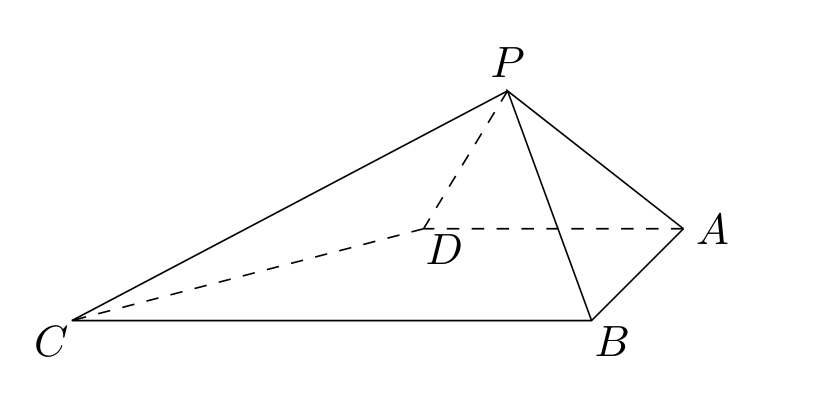
\includegraphics[width=5.8cm]{GaoKao/images/2013/syllabus_science/q19_fig1.png}
\end{center}

        \item 甲，乙，丙三人进行羽毛球练习赛，其中两人比赛，另一人当裁判. 每局比赛结束时，负的一方在下一局当裁判. 设各局中双方获胜的概率均为 \(\frac{1}{2}\)，各局比赛的结果都相互独立，第1局甲当裁判.

\begin{enumerate}
\item 求第 4 局甲当裁判的概率；
\item \(X\) 表示前 4 局中乙当裁判的次数. 求 \(X\) 的数学期望.
\end{enumerate}

        \item 已知双曲线 \(C:\frac{x^2}{a^2}-\frac{y^2}{b^2}=1\)（\(a>0,b>0\)）的左，右焦点分别为 \(F_1\)，\(F_2\)，离心率为 3，直线 \(y=2\) 与 \(C\) 的两个交点间的距离为 \(\sqrt{6}\).

\begin{enumerate}
\item 求 \(a\)，\(b\)；
\item 设过 \(F_2\) 的直线 \(l\) 与 \(C\) 的左，右两支分别交于 \(A\)，\(B\) 两点，且 \(|AF_1|=|BF_1|\)，证明：\(|AF_2|\)，\(|AB|\)，\(|BF_2|\) 成等比数列.
\end{enumerate}

    \end{enumerate}

\end{description}

\begin{description}

    \item[四、选考题]

    \begin{enumerate}[leftmargin=5pt]

      \addtocounter{enumi}{+21}

        \item 已知函数 \(f(x)=\ln\left(1+x\right)-\frac{x(1+\lambda x)}{1+x}\).

\begin{enumerate}
\item 若 \(x\geqslant0\) 时 \(f(x)\leqslant0\)，求 \(\lambda\) 的最小值；
\item 设数列 \(\{a_n\}\) 的通项 \(a_n=1+\frac{1}{2}+\frac{1}{3}+\dots+\frac{1}{n}\)，证明：\(a_{2n}-a_n+\frac{1}{4n}>\ln2\).
\end{enumerate}

    \end{enumerate}

\end{description}


\subsection{2013年大纲卷（文）}\label{gk:2013年大纲卷（文）}

\begin{description}

    \item[一、选择题]

    \begin{enumerate}[leftmargin=5pt]

        \item 设全集 \(U = \{1, 2, 3, 4, 5\}\)，集合 \(A = \{1, 2\}\)，则 \(\complement_U A =\)（\quad）

        {\centering\begin{tabular*}{\linewidth}{@{}@{\extracolsep{\fill}}llll@{}}
          \text{A. }\( \{1, 2\} \)  &  \text{B. }\(\{3,4,5\}\)  &  \text{C. }\( \{1, 2, 3, 4, 5\} \)  &  \text{D. }\(\varnothing\)
        \end{tabular*}\par}

        \item 已知 \(\alpha\) 是第二象限角，\(\sin \alpha = \frac{5}{13}\)，则 \(\cos \alpha =\)（\quad）

        {\centering\begin{tabular*}{\linewidth}{@{}@{\extracolsep{\fill}}llll@{}}
          \text{A. }\(-\frac{12}{13}\)  &  \text{B. }\(-\frac{5}{13}\)  &  \text{C. }\(\frac{5}{13}\)  &  \text{D. }\(\frac{12}{13}\)
        \end{tabular*}\par}

        \item 已知向量 \(\bm{m} = (\lambda + 1, 1)\)，\(\bm{n} = (\lambda + 2, 2)\)，若 \((\bm{m} + \bm{n}) \perp (\bm{m} - \bm{n})\)，则 \(\lambda =\)（\quad）

        {\centering\begin{tabular*}{\linewidth}{@{}@{\extracolsep{\fill}}llll@{}}
          \text{A. }\(-4\)  &  \text{B. }\(-3\)  &  \text{C. }\(-2\)  &  \text{D. }\(-1\)
        \end{tabular*}\par}

        \item 不等式 \( |x^2 - 2| < 2 \) 的解集是（\quad）

        {\centering\begin{tabular*}{\linewidth}{@{}@{\extracolsep{\fill}}llll@{}}
          \text{A. }\((-1, 1)\)  &  \text{B. }\((-2, 2)\)  &  \text{C. }\((-1,0)\cup (0,1)\)  &  \text{D. }\((-2,0)\cup (0,2)\)
        \end{tabular*}\par}

        \item \((x + 2)^{8}\) 的展开式中 \(x^{6}\) 的系数是（\quad）

        {\centering\begin{tabular*}{\linewidth}{@{}@{\extracolsep{\fill}}llll@{}}
          \text{A. }\(28\)  &  \text{B. }\(56\)  &  \text{C. }\(112\)  &  \text{D. }\(224\)
        \end{tabular*}\par}

        \item 函数 \( f(x) = \log_2\left(1 + \frac{1}{x}\right)  \) （\(x > 0\)）的反函数 \( f^{-1}(x) = \)（\quad）

        {\centering\begin{tabular*}{\linewidth}{@{}@{\extracolsep{\fill}}llll@{}}
          \text{A. }\(\frac{1}{2^{x} - 1} \)（\(x > 0\)）  &  \text{B. }\(\frac{1}{2^{x} - 1} \)（\(x\neq 0\)）  &  \text{C. }\(2^{x} - 1 \)（\(x \in \mathbb{R}\)）  &  \text{D. }\(2^{x} - 1 \)（\(x > 0\)）
        \end{tabular*}\par}

        \item 已知数列 \( \{a_{n}\} \) 满足 \(3a_{n+1} + a_{n} = 0\)，\(a_{2} = -\frac{4}{3}\)，则 \( \{a_{n}\} \) 的前 10 项和等于（\quad）

        {\centering\begin{tabular*}{\linewidth}{@{}@{\extracolsep{\fill}}llll@{}}
          \text{A. }\(-6(1 - 3^{-10})\)  &  \text{B. }\(\frac{1}{9}(1 - 3^{10})\)  &  \text{C. }\(3(1 - 3^{-10})\)  &  \text{D. }\(3(1 + 3^{-10})\)
        \end{tabular*}\par}

        \item 已知 \(F_{1}(-1,0)\)，\(F_{2}(1,0)\) 是椭圆 \(C\) 的两个焦点，过 \(F_{2}\) 且垂直于 \(x\) 轴的直线交 \(C\) 于 \(A\)，\(B\) 两点，且 \(|AB| = 3\)，则 \(C\) 的方程为（\quad）

        {\centering\begin{tabular*}{\linewidth}{@{}@{\extracolsep{\fill}}llll@{}}
          \text{A. }\(\frac{x^2}{2} + y^2 = 1\)  &  \text{B. }\(\frac{x^2}{3} + \frac{y^2}{2} = 1\)  &  \text{C. }\(\frac{x^2}{4} + \frac{y^2}{3} = 1\)  &  \text{D. }\(\frac{x^2}{5} + \frac{y^2}{4} = 1\)
        \end{tabular*}\par}

        \item 若函数 \( y = \sin (\omega x + \varphi)  \) （\(\omega > 0\)）的部分图像如图所示，则 \( \omega = \)（\quad）

\begin{center}
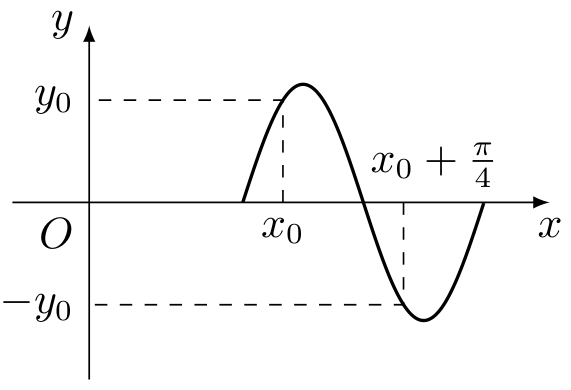
\includegraphics[width=7.3cm]{GaoKao/images/2013/syllabus_liberal/q9_fig1.png}
\end{center}

        {\centering\begin{tabular*}{\linewidth}{@{}@{\extracolsep{\fill}}llll@{}}
          \text{A. }\(5\)  &  \text{B. }\(4\)  &  \text{C. }\(3\)  &  \text{D. }\(2\)
        \end{tabular*}\par}

        \item 已知曲线 \( y = x^4 + ax^2 + 1 \) 在点 \((-1, a + 2)\) 处切线的斜率为 8，则 \( a = \)（\quad）

        {\centering\begin{tabular*}{\linewidth}{@{}@{\extracolsep{\fill}}llll@{}}
          \text{A. }\(9\)  &  \text{B. }\(6\)  &  \text{C. }\(-9\)  &  \text{D. }\(-6\)
        \end{tabular*}\par}

        \item 已知正四棱柱 \(ABCD - A_{1}B_{1}C_{1}D_{1}\) 中，\(AA_{1} = 2AB\)，则 \(CD\) 与平面 \(BDC_{1}\) 所成角的正弦值等于（\quad）

        {\centering\begin{tabular*}{\linewidth}{@{}@{\extracolsep{\fill}}llll@{}}
          \text{A. }\(\frac{2}{3}\)  &  \text{B. }\(\frac{\sqrt{3}}{3}\)  &  \text{C. }\(\frac{\sqrt{2}}{3}\)  &  \text{D. }\(\frac{1}{3}\)
        \end{tabular*}\par}

        \item 已知抛物线 \(C: y^{2} = 8x\) 与点 \(M(-2, 2)\)，过 \(C\) 的焦点且斜率为 \(k\) 的直线与 \(C\) 交于 \(A\)，\(B\) 两点，若 \(\overrightarrow{MA} \cdot \overrightarrow{MB} = 0\)，则 \(k =\)（\quad）

        {\centering\begin{tabular*}{\linewidth}{@{}@{\extracolsep{\fill}}llll@{}}
          \text{A. }\(\frac{1}{2}\)  &  \text{B. }\( \frac{\sqrt{2}}{2} \)  &  \text{C. }\(\sqrt{2}\)  &  \text{D. }\(2\)
        \end{tabular*}\par}

    \end{enumerate}

\end{description}

\begin{description}

    \item[二、填空题]

    \begin{enumerate}[leftmargin=5pt]

      \addtocounter{enumi}{+12}

        \item 设 \( f(x) \) 是以 2 为周期的函数，且当 \( x \in [1,3) \) 时，\( f(x) = x - 2 \)，则 \( f(-1) = \)\rule[-0.3ex]{3em}{0.4pt}.

        \item 从进入决赛的6名选手中决出1名一等奖，2名二等奖，3名三等奖，则可能的决赛结果共有\rule[-0.3ex]{3em}{0.4pt} 种.

        \item 若 \(x\)，\(y\) 满足的约束条件 \(\begin{cases}
x\geqslant 0,\\
x + 3y\geqslant 4,\\
3x + y\leqslant 4.
\end{cases}\) 则 \(z = -x + y\) 的最小值为\rule[-0.3ex]{3em}{0.4pt}.

        \item 已知圆 \(O\) 和圆 \(K\) 是球 \(O\) 的大圆和小圆，其公共弦长等于球 \(O\) 的半径，\(OK = \frac{3}{2}\)，且圆 \(O\) 与圆 \(K\) 所在的平面所成的一个二面角为 \(60^{\circ}\)，则球 \(O\) 的表面积等于\rule[-0.3ex]{3em}{0.4pt}.

    \end{enumerate}

\end{description}

\begin{description}

    \item[三、解答题]

    \begin{enumerate}[leftmargin=5pt]

      \addtocounter{enumi}{+16}

        \item 等差数列 \(\{a_{n}\}\) 中，\(a_{7} = 4\)，\(a_{19} = 2a_{9}\).

\begin{enumerate}
\item 求 \(\{a_{n}\}\) 的通项公式；
\item 设 \(b_n = \frac{1}{na_n}\)，求数列 \(\{b_n\}\) 的前 \(n\) 项和 \(S_n\).
\end{enumerate}

        \item 设 \(\triangle ABC\) 的内角 \(A\)，\(B\)，\(C\) 的对边分别为 \(a\)，\(b\)，\(c\)，\((a + b + c)(a - b + c) = ac\).

\begin{enumerate}
\item 求 \(B\)；
\item 若 \(\sin A \sin C = \frac{\sqrt{3} - 1}{4}\)，求 \(C\).
\end{enumerate}

        \item 如图，四棱锥 \(P - ABCD\) 中，\(\angle ABC = \angle BAD = 90^{\circ}\)，\(BC = 2AD\)，\(\triangle PAB\) 与 \(\triangle PAD\) 都是边长为 2 的等边三角形.

\begin{enumerate}
\item 证明：\(PB \perp CD\)；
\item 求点 \(A\) 到平面 \(PCD\) 的距离.
\end{enumerate}

\begin{center}
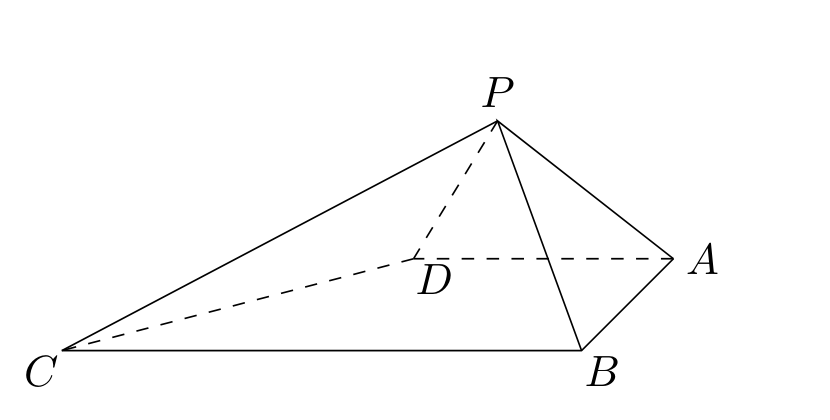
\includegraphics[width=7.0cm]{GaoKao/images/2013/syllabus_liberal/q19_fig1.png}
\end{center}

        \item 甲，乙，丙三人进行羽毛球练习赛，其中两人比赛，另一人当裁判. 每局比赛结束时，负的一方在下一局当裁判. 设各局中双方获胜的概率均为 \(\frac{1}{2}\)，各局比赛的结果都相互独立，第1局甲当裁判.

\begin{enumerate}
\item 求第 4 局甲当裁判的概率；
\item 求前 4 局中乙恰好当 1 次裁判的概率.
\end{enumerate}

        \item 已知函数 \( f(x) = x^3 + 3ax^2 + 3x + 1 \).

\begin{enumerate}
\item 当 \(a = -\sqrt{2}\) 时，讨论 \(f(x)\) 的单调性；
\item 若 \(x \in [2, +\infty)\) 时，\(f(x) \geqslant 0\)，求 \(a\) 的取值范围.
\end{enumerate}

    \end{enumerate}

\end{description}

\begin{description}

    \item[四、选考题]

    \begin{enumerate}[leftmargin=5pt]

      \addtocounter{enumi}{+21}

        \item 已知双曲线 \(C: \frac{x^2}{a^2} - \frac{y^2}{b^2} = 1 \) （\(a > 0, b > 0\)）的左，右焦点分别为 \(F_1\)，\(F_2\)，离心率为 3，直线 \(y = 2\) 与 \(C\) 的两个交点间的距离为 \(\sqrt{6}\).

\begin{enumerate}
\item 求 \(a\)，\(b\)；
\item 设过 \(F_{2}\) 的直线 \(l\) 与 \(C\) 的左，右两支分别交于 \(A\)，\(B\) 两点，且 \(|AF_{1}| = |BF_{1}|\)，证明：\(|AF_{2}|\)，\(|AB|\)，\(|BF_{2}|\) 成等比数列.
\end{enumerate}

    \end{enumerate}

\end{description}


\subsection{2013年全国I卷（理）}\label{gk:2013年全国I卷（理）}

\begin{description}

    \item[一、选择题]

    \begin{enumerate}[leftmargin=5pt]

        \item 已知集合 \(A = \{x \mid x^2 - 2x > 0\}\)，\(B = \{x \mid -\sqrt{5} < x < \sqrt{5}\}\)，则（\quad）

        {\centering\begin{tabular*}{\linewidth}{@{}@{\extracolsep{\fill}}llll@{}}
          \text{A. }\(A \cap B = \varnothing\)  &  \text{B. }\(A \cup B = \mathbb{R}\)  &  \text{C. }\(B \subseteq A\)  &  \text{D. }\(A \subseteq B\)
        \end{tabular*}\par}

        \item 若复数 \(z\) 满足 \(\left(3 - 4\i\right)z = \left|4 + 3\i\right|\)，则 \(z\) 的虚部为（\quad）

        {\centering\begin{tabular*}{\linewidth}{@{}@{\extracolsep{\fill}}llll@{}}
          \text{A. }\(-4\)  &  \text{B. }\(-\frac{4}{5}\)  &  \text{C. }4  &  \text{D. }\(\frac{4}{5}\)
        \end{tabular*}\par}

        \item 为了解某地区的中小学生视力情况，拟从该地区的中小学生中抽取部分学生进行调查，事先已了解到该地区小学，初中，高中三个学段学生的视力情况有较大差异，而男女生视力情况差异不大，在下面的抽样方法中，最合理的抽样方法是（\quad）

        {\centering\begin{tabular*}{\linewidth}{@{}@{\extracolsep{\fill}}llll@{}}
          \text{A. }简单随机抽样  &  \text{B. }按性别分层抽样  &  \text{C. }按学段分层抽样  &  \text{D. }系统抽样
        \end{tabular*}\par}

        \item 已知双曲线 \(C: \frac{x^2}{a^2} - \frac{y^2}{b^2} = 1\left(a > 0, b > 0\right)\) 的离心率为 \(\frac{\sqrt{5}}{2}\)，则 \(C\) 的渐近线方程为（\quad）

        {\centering\begin{tabular*}{\linewidth}{@{}@{\extracolsep{\fill}}llll@{}}
          \text{A. }\(y = \pm \frac{1}{4} x\)  &  \text{B. }\(y = \pm \frac{1}{3}x\)  &  \text{C. }\( y = \pm \frac{1}{2} x \)  &  \text{D. }\(y = \pm x\)
        \end{tabular*}\par}

        \item 执行下面的程序框图，若输入的 \(t \in \left[-1, 3\right]\)，则输出的 \(s\) 属于（\quad）

\begin{center}
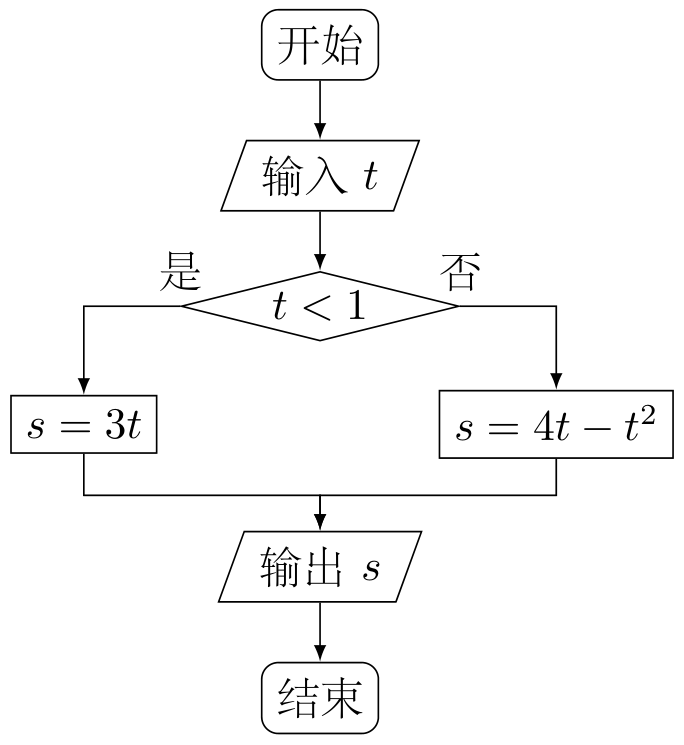
\includegraphics[width=2.0cm]{GaoKao/images/2013/new_curriculum_paper_1_science/q5_fig1.png}
\end{center}

        {\centering\begin{tabular*}{\linewidth}{@{}@{\extracolsep{\fill}}llll@{}}
          \text{A. }\(\left[-3, 4\right]\)  &  \text{B. }\(\left[-5, 2\right]\)  &  \text{C. }\(\left[-4, 3\right]\)  &  \text{D. }\(\left[-2, 5\right]\)
        \end{tabular*}\par}

        \item 如图，有一个水平放置的透明无盖的正方体容器，容器高 \(8\mathrm{~cm}\)，将一个球放在容器口，再向容器内注水，当球面恰好接触水面时测得水深为 \(6\mathrm{~cm}\)，如果不计容器的厚度，则球的体积为（\quad）

\begin{minipage}{\linewidth}
\begin{center}
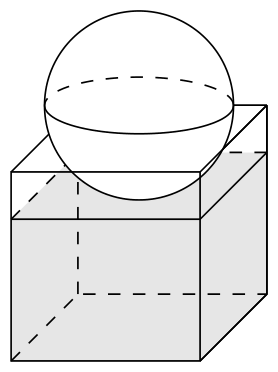
\includegraphics[width=0.42\linewidth]{GaoKao/images/2013/new_curriculum_paper_1_science/q6_fig1.png}
\end{center}
\end{minipage}

        {\centering\begin{tabular*}{\linewidth}{@{}@{\extracolsep{\fill}}llll@{}}
          \text{A. }\(\frac{500\pi}{3}\mathrm{~cm}^{3}\)  &  \text{B. }\(\frac{866\pi}{3}\mathrm{~cm}^{3}\)  &  \text{C. }\(\frac{1372\pi}{3}\mathrm{~cm}^{3}\)  &  \text{D. }\(\frac{2048\pi}{3}\mathrm{~cm}^{3}\)
        \end{tabular*}\par}

        \item 设等差数列 \(\{a_{n}\}\) 的前 \(n\) 项和为 \(S_{n}\)，\(S_{m-1} = -2\)，\(S_{m} = 0\)，\(S_{m+1} = 3\)，则 \(m =\)（\quad）

        {\centering\begin{tabular*}{\linewidth}{@{}@{\extracolsep{\fill}}llll@{}}
          \text{A. }3  &  \text{B. }4  &  \text{C. }5  &  \text{D. }6
        \end{tabular*}\par}

        \item 某几何体的三视图如图所示，则该几何的体积为（\quad）

\begin{center}
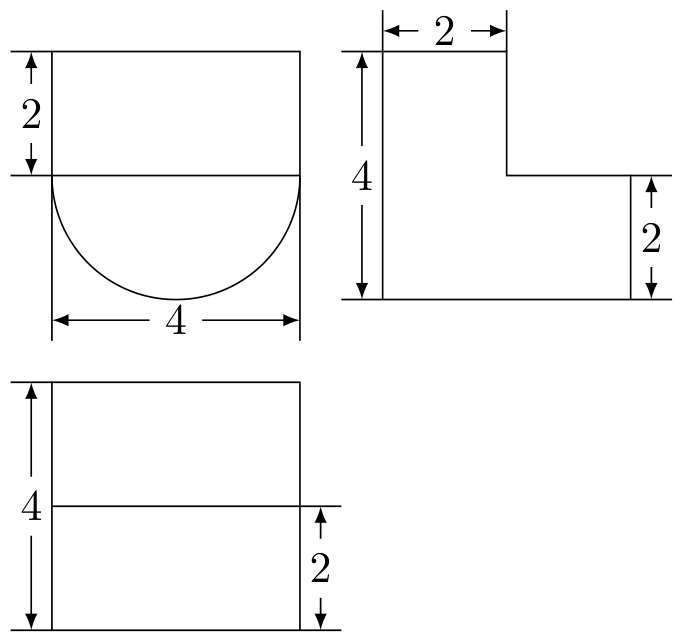
\includegraphics[width=6.8cm]{GaoKao/images/2013/new_curriculum_paper_1_science/q8_fig1.png}
\end{center}

        {\centering\begin{tabular*}{\linewidth}{@{}@{\extracolsep{\fill}}llll@{}}
          \text{A. }\(16 + 8\pi\)  &  \text{B. }\(8 + 8\pi\)  &  \text{C. }\(16 + 16\pi\)  &  \text{D. }\(8 + 16\pi\)
        \end{tabular*}\par}

        \item 设 \(m\) 为正整数，\(\left(x + y\right)^{2m}\) 展开式的二项式系数的最大值为 \(a\)，\(\left(x + y\right)^{2m + 1}\) 展开式的二项式系数的最大值为 \(b\)，若 \(13a = 7b\)，则 \(m =\)（\quad）

        {\centering\begin{tabular*}{\linewidth}{@{}@{\extracolsep{\fill}}llll@{}}
          \text{A. }5  &  \text{B. }6  &  \text{C. }7  &  \text{D. }8
        \end{tabular*}\par}

        \item 已知椭圆 \(E: \frac{x^2}{a^2} + \frac{y^2}{b^2} = 1\left(a > b > 0\right)\) 的右焦点为 \(F\left(3,0\right)\)，过点 \(F\) 的直线交 \(E\) 于 \(A\)，\(B\) 两点. 若 \(AB\) 的中点坐标为 \(\left(1, -1\right)\)，则 \(E\) 的方程为（\quad）

        {\centering\begin{tabular*}{\linewidth}{@{}@{\extracolsep{\fill}}llll@{}}
          \text{A. }\(\frac{x^2}{45} + \frac{y^2}{36} = 1\)  &  \text{B. }\(\frac{x^2}{36} + \frac{y^2}{27} = 1\)  &  \text{C. }\(\frac{x^2}{27} + \frac{y^2}{18} = 1\)  &  \text{D. }\(\frac{x^2}{18} + \frac{y^2}{9} = 1\)
        \end{tabular*}\par}

        \item 已知函数 \( f(x) = \begin{cases}
-x^2 + 2x, & x \leqslant 0,\\
\ln\left(x + 1\right), & x > 0,
\end{cases} \) 若 \( |f(x)| \geqslant ax \)，则 \( a \) 的取值范围是（\quad）

        {\centering\begin{tabular*}{\linewidth}{@{}@{\extracolsep{\fill}}llll@{}}
          \text{A. }\(\left(-\infty, 0\right]\)  &  \text{B. }\(\left(-\infty, 1\right]\)  &  \text{C. }\(\left[-2, 1\right]\)  &  \text{D. }\(\left[-2, 0\right]\)
        \end{tabular*}\par}

        \item 设 \(\triangle A_{n}B_{n}C_{n}\) 的三边长分别为 \(a_{n}\)，\(b_{n}\)，\(c_{n}\)，\(\triangle A_{n}B_{n}C_{n}\) 的面积为 \(S_{n}\)，\(n = 1\)，\(2\)，\(3\)，\(\cdots\)，若 \(b_{1} > c_{1}\)，\(b_{1} + c_{1} = 2a_{1}\)，\(a_{n+1} = a_{n}\)，\(b_{n+1} = \frac{c_{n} + a_{n}}{2}\)，\(c_{n+1} = \frac{b_{n} + a_{n}}{2}\)，则（\quad）

        {\centering\begin{tabular*}{\linewidth}{@{}@{\extracolsep{\fill}}llll@{}}
          \text{A. }\(\{S_{n}\}\) 为递减数列  &  \text{B. }\(\{S_{n}\}\) 为递增数列  &  \text{C. }\(\{S_{2n - 1}\}\) 为递增数列，\(\{S_{2n}\}\) 为递减数列  &  \text{D. }\(\{S_{2n - 1}\}\) 为递减数列，\(\{S_{2n}\}\) 为递增数列
        \end{tabular*}\par}

    \end{enumerate}

\end{description}

\begin{description}

    \item[二、填空题]

    \begin{enumerate}[leftmargin=5pt]

      \addtocounter{enumi}{+12}

        \item 已知两个单位向量 \(\bm{a}\)，\(\bm{b}\) 的夹角为 \(60^{\circ}\)，\(\bm{c} = t\bm{a} + (1 - t)\bm{b}\)，若 \(\bm{b} \cdot \bm{c} = 0\)，则 \(t =\rule[-0.3ex]{3em}{0.4pt}\).

        \item 若数列 \(\{a_{n}\}\) 的前 \(n\) 项和为 \(S_{n}=\frac{2}{3}a_{n}+\frac{1}{3}\)，则数列 \(\{a_{n}\}\) 的通项公式是 \(a_{n}=\)\rule[-0.3ex]{3em}{0.4pt}.

        \item 设当 \(x = \theta\) 时，函数 \(f(x) = \sin x - 2\cos x\) 取得最大值，则 \(\cos \theta =\rule[-0.3ex]{3em}{0.4pt}\).

        \item 若函数 \( f(x) = \left(1 - x^2\right)\left(x^2 + ax + b\right) \) 的图象关于直线 \( x = -2 \) 对称，则 \( f(x) \) 的最大值是\rule[-0.3ex]{3em}{0.4pt}.

    \end{enumerate}

\end{description}

\begin{description}

    \item[三、解答题]

    \begin{enumerate}[leftmargin=5pt]

      \addtocounter{enumi}{+16}

        \item 如图，在 \(\triangle ABC\) 中，\(\angle ABC = 90^{\circ}\)，\(AB = \sqrt{3}\)，\(BC = 1\)，\(P\) 为 \(\triangle ABC\) 内一点，\(\angle BPC = 90^{\circ}\).

\begin{enumerate}
\item 若 \(PB = \frac{1}{2}\)，求 \(PA\)；
\item 若 \(\angle APB = 150^{\circ}\)，求 \(\tan \angle PBA\).
\end{enumerate}

\begin{center}
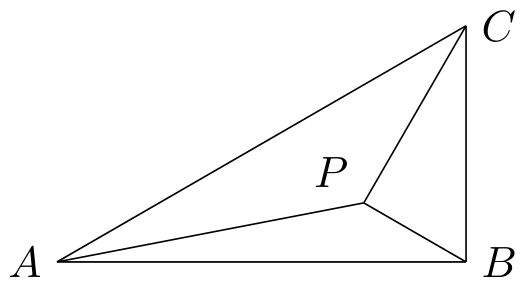
\includegraphics[width=6.5cm]{GaoKao/images/2013/new_curriculum_paper_1_science/q17_fig1.png}
\end{center}

        \item 如图，三棱柱 \(ABC - A_{1}B_{1}C_{1}\) 中，\(CA = CB\)，\(AB = AA_{1}\)，\(\angle BAA_{1} = 60^{\circ}\).

\begin{enumerate}
\item 证明： \(AB \perp A_{1}C\)；
\item 若平面 \( ABC \perp \) 平面 \(AA_{1}B_{1}B\)，\( AB = CB \)，求直线 \(A_{1}C\) 与平面 \(BB_{1}C_{1}C\) 所成角的正弦值.
\end{enumerate}

\begin{center}
\begin{center}
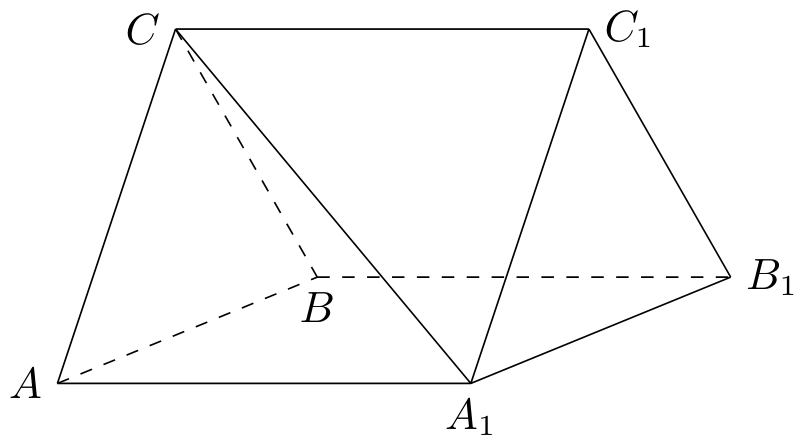
\includegraphics[width=8.5cm]{GaoKao/images/2013/new_curriculum_paper_1_science/q18_fig1.png}
\end{center}
\end{center}

        \item 一批产品需要进行质量检验，检验方案是：先从这批产品中任取 \(4\) 件作检验，这 \(4\) 件产品中优质品的件数记为 \(n\). 如果 \(n = 3\)，再从这批产品中任取 \(4\) 件作检验，若都为优质品，则这批产品通过检验；如果 \(n = 4\)，再从这批产品中任取 \(1\) 件作检验，若为优质品，则这批产品通过检验；其他情况下，这批产品都不能通过检验. 假设这批产品的优质品率为 \(50\%\). 即取出的产品是优质品的概率都为 \(\frac{1}{2}\)，且各件产品是否为优质品相互独立.
\begin{enumerate}
\item 求这批产品通过检验的概率；
\item 已知每件产品检验费用为 \(100\text{ 元}\)，凡抽取的每件产品都需要检验，对这批产品作质量检验所需的费用记为 \(X\)（单位：元），求 \(X\) 的分布列及数学期望.
\end{enumerate}

        \item 已知圆 \(M: \left(x + 1\right)^2 + y^2 = 1\)，圆 \(N: \left(x - 1\right)^2 + y^2 = 9\)，动圆 \(P\) 与圆 \(M\) 外切并与圆 \(N\) 内切，圆心 \(P\) 的轨迹为曲线 \(C\).
\begin{enumerate}
\item 求 \(C\) 的方程；
\item \(l\) 是与圆 \(P\)，圆 \(M\) 都相切的一条直线，\(l\) 与曲线 \(C\) 交于 \(A\)，\(B\) 两点，当圆 \(P\) 的半径最长时，求 \(|AB|\).
\end{enumerate}

        \item 设函数 \(f(x) = x^2 + ax + b\)，\(g(x) = {\mathrm{e}}^x\left(cx + d\right)\)，若曲线 \(y = f(x)\) 和曲线 \(y = g(x)\) 都过点 \(P\left(0,2\right)\)，且在点 \(P\) 处有相同的切线 \(y = 4x + 2\).
\begin{enumerate}
\item 求 \(a\)，\(b\)，\(c\)，\(d\) 的值；
\item 若 \(x \geqslant -2\) 时，\(f(x) \leqslant kg(x)\)，求 \(k\) 的取值范围.
\end{enumerate}

        \item 如图，直线 \(AB\) 为圆的切线，切点为 \(B\)，点 \(C\) 在圆上，\(\angle ABC\) 的角平分线 \(BE\) 交圆于点 \(E\)，\(DB\) 垂直 \(BE\) 交圆于 \(D\).

\begin{enumerate}
\item 证明： \(DB = DC\)；
\item 设圆的半径为 \(1\)，\(BC = \sqrt{3}\)，延长 \(CE\) 交 \(AB\) 于点 \(F\)，求 \(\triangle BCF\) 外接圆的半径.
\end{enumerate}

\begin{center}
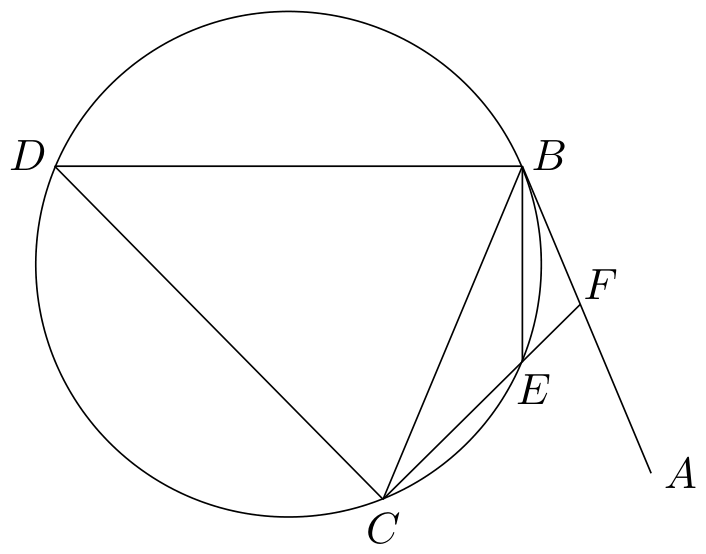
\includegraphics[width=8.5cm]{GaoKao/images/2013/new_curriculum_paper_1_science/q22_fig1.png}
\end{center}

        \item 已知曲线 \(C_1\) 的参数方程为 \(\begin{cases}
x = 4 + 5\cos t,\\
y = 5 + 5\sin t,
\end{cases}\) （\(t\) 为参数），以坐标原点为极点，\(x\) 轴的正半轴为极轴建立极坐标系. 曲线 \(C_2\) 的极坐标方程为 \(\rho = 2\sin \theta\).
\begin{enumerate}
\item 把 \(C_1\) 的参数方程化为极坐标方程；
\item 求 \(C_1\) 与 \(C_2\) 交点的极坐标 \(\left(\rho \geqslant 0, 0 \leqslant \theta < 2\pi\right)\).
\end{enumerate}

        \item 已知函数 \( f(x) = |2x - 1| + |2x + a| \)，\( g(x) = x + 3 \).
\begin{enumerate}
\item 当 \(a = -2\) 时，求不等式 \(f(x) < g(x)\) 的解集；
\item 设 \(a > -1\)，且当 \(x \in \left[-\frac{a}{2}, \frac{1}{2}\right]\) 时，\(f(x) \leqslant g(x)\)，求 \(a\) 的取值范围.
\end{enumerate}

    \end{enumerate}

\end{description}


\subsection{2013年全国I卷（文）}\label{gk:2013年全国I卷（文）}

\begin{description}

    \item[一、选择题]

    \begin{enumerate}[leftmargin=5pt]

        \item 已知集合 \(A = \{1, 2, 3, 4\}\)，\(B = \{x \mid x = n^2, n \in A\}\)，则 \(A \cap B =\)（\quad）

        {\centering\begin{tabular*}{\linewidth}{@{}@{\extracolsep{\fill}}llll@{}}
          \text{A. }\(\{1, 4\}\)  &  \text{B. }\(\{2, 3\}\)  &  \text{C. }\(\{9, 16\}\)  &  \text{D. }\(\{1, 2\}\)
        \end{tabular*}\par}

        \item \(\frac{1 + 2\i}{(1 - \i)^2} =\)（\quad）

        {\centering\begin{tabular*}{\linewidth}{@{}@{\extracolsep{\fill}}llll@{}}
          \text{A. }\(-1 - \frac{1}{2}\i\)  &  \text{B. }\(-1 + \frac{1}{2}\i\)  &  \text{C. }\(1 + \frac{1}{2}\i\)  &  \text{D. }\(1 - \frac{1}{2}\i\)
        \end{tabular*}\par}

        \item 从 \(1\)，\(2\)，\(3\)，\(4\) 中任取 \(2\) 个不同的数，则取出的 \(2\) 个数之差的绝对值为 \(2\) 的概率是（\quad）

        {\centering\begin{tabular*}{\linewidth}{@{}@{\extracolsep{\fill}}llll@{}}
          \text{A. }\(\frac{1}{2}\)  &  \text{B. }\(\frac{1}{3}\)  &  \text{C. }\( \frac{1}{4} \)  &  \text{D. }\(\frac{1}{6}\)
        \end{tabular*}\par}

        \item 已知双曲线 \(C: \frac{x^2}{a^2} - \frac{y^2}{b^2} = 1\left(a > 0, b > 0\right)\) 的离心率为 \(\frac{\sqrt{5}}{2}\)，则 \(C\) 的渐近线方程为（\quad）

        {\centering\begin{tabular*}{\linewidth}{@{}@{\extracolsep{\fill}}llll@{}}
          \text{A. }\(y = \pm \frac{1}{4} x\)  &  \text{B. }\(y = \pm \frac{1}{3} x\)  &  \text{C. }\(y = \pm \frac{1}{2} x\)  &  \text{D. }\(y = \pm x\)
        \end{tabular*}\par}

        \item 已知命题 \(p\)：\(\forall x \in \mathbb{R}\)，\(2^x < 3^x\)；命题 \(q\)：\(\exists x \in \mathbb{R}\)，\(x^3 = 1 - x^2\)，则下列命题中为真命题的是（\quad）

        {\centering\begin{tabular*}{\linewidth}{@{}@{\extracolsep{\fill}}llll@{}}
          \text{A. }\(p \wedge q\)  &  \text{B. }\(\neg p \land q\)  &  \text{C. }\(p \wedge \neg q\)  &  \text{D. }\(\neg p \land \neg q\)
        \end{tabular*}\par}

        \item 设首项为 \(1\)，公比为 \(\frac{2}{3}\) 的等比数列 \(\{a_n\}\) 的前 \(n\) 项和为 \(S_n\)，则（\quad）

        {\centering\begin{tabular*}{\linewidth}{@{}@{\extracolsep{\fill}}llll@{}}
          \text{A. }\(S_{n} = 2a_{n} - 1\)  &  \text{B. }\(S_{n} = 3a_{n} - 2\)  &  \text{C. }\(S_{n} = 4 - 3a_{n}\)  &  \text{D. }\(S_{n} = 3 - 2a_{n}\)
        \end{tabular*}\par}

        \item 执行下面的程序框图，若输入的 \(t \in [-1,3]\)，则输出的 \(s\) 属于（\quad）

\begin{center}
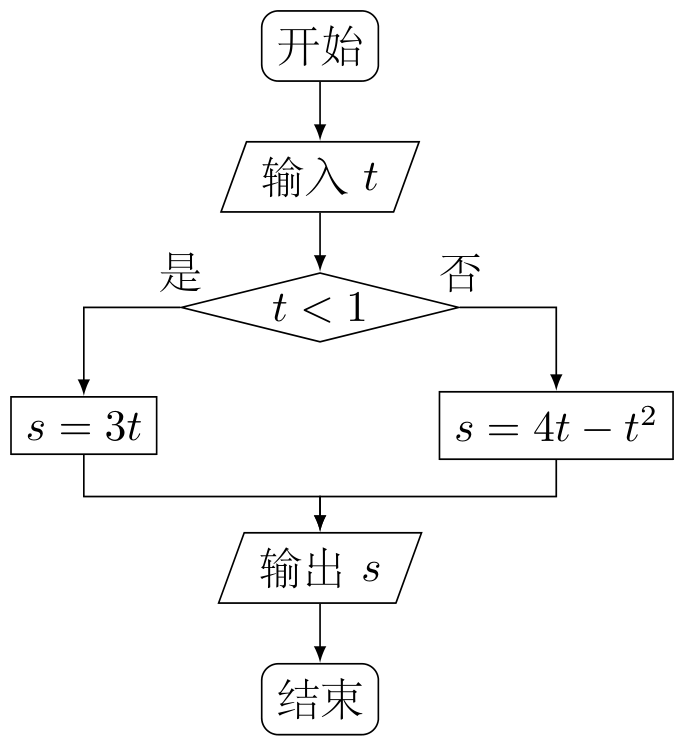
\includegraphics[width=3.6cm]{GaoKao/images/2013/new_curriculum_paper_1_liberal/q7_fig1.png}
\end{center}

        {\centering\begin{tabular*}{\linewidth}{@{}@{\extracolsep{\fill}}llll@{}}
          \text{A. }\([-3, 4]\)  &  \text{B. }\([-5, 2]\)  &  \text{C. }\([-4,3]\)  &  \text{D. }\([-2,5]\)
        \end{tabular*}\par}

        \item \(O\) 为坐标原点，\(F\) 为抛物线 \(C: y^{2} = 4\sqrt{2} x\) 的焦点，\(P\) 为 \(C\) 上一点，若 \(|PF| = 4\sqrt{2}\)，则 \(\triangle POF\) 的面积为（\quad）

        {\centering\begin{tabular*}{\linewidth}{@{}@{\extracolsep{\fill}}llll@{}}
          \text{A. }\(2\)  &  \text{B. }\(2\sqrt{2}\)  &  \text{C. }\(2\sqrt{3}\)  &  \text{D. }\(4\)
        \end{tabular*}\par}

        \item 函数 \(f(x) = (1 - \cos x)\sin x\) 在 \(\left[-\pi,\pi\right]\) 的图象大致为（\quad）

        {\centering\begin{tabular*}{\linewidth}{@{}@{\extracolsep{\fill}}cccc@{}}
          \text{A. }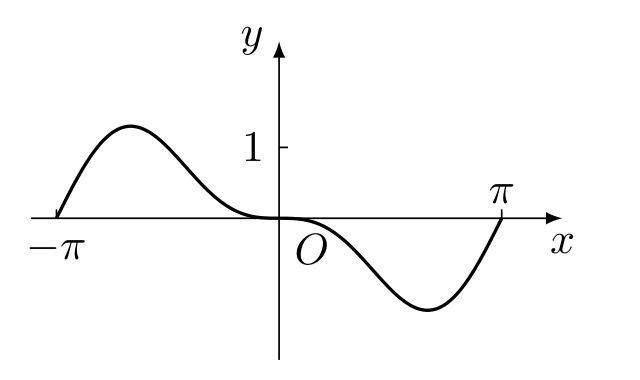
\includegraphics[width=0.15\paperwidth]{GaoKao/images/2013/new_curriculum_paper_1_liberal/q9_choice_a.png}  &  \text{B. }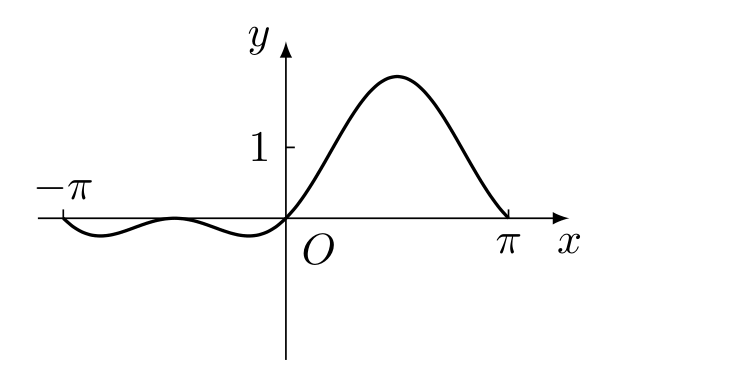
\includegraphics[width=0.15\paperwidth]{GaoKao/images/2013/new_curriculum_paper_1_liberal/q9_choice_b.png}  &  \text{C. }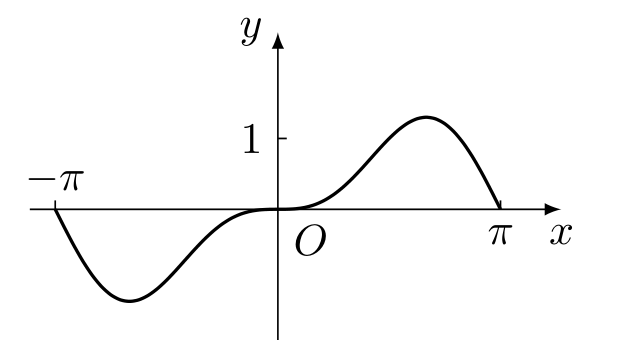
\includegraphics[width=0.15\paperwidth]{GaoKao/images/2013/new_curriculum_paper_1_liberal/q9_choice_c.png}  &  \text{D. }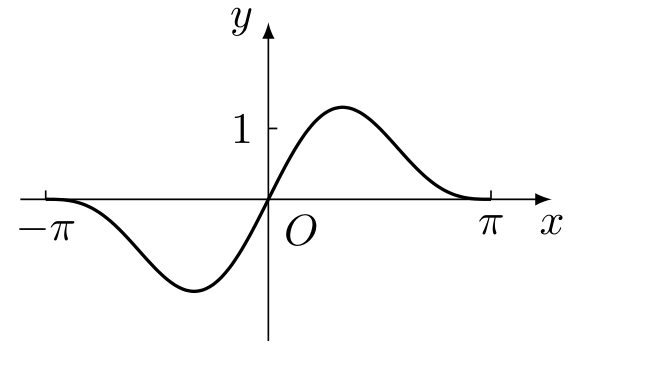
\includegraphics[width=0.15\paperwidth]{GaoKao/images/2013/new_curriculum_paper_1_liberal/q9_choice_d.png}
        \end{tabular*}\par}

        \item 已知锐角三角形 \(ABC\) 的内角 \(A\)，\(B\)，\(C\) 的对边分别为 \(a\)，\(b\)，\(c\)，\(2\cos^{2} A + \cos 2A = 0\)，\(a = 7\)，\(c = 6\)，则 \(b =\)（\quad）

        {\centering\begin{tabular*}{\linewidth}{@{}@{\extracolsep{\fill}}llll@{}}
          \text{A. }\(10\)  &  \text{B. }\(9\)  &  \text{C. }\(8\)  &  \text{D. }\(5\)
        \end{tabular*}\par}

        \item 某几何体的三视图如图所示，则该几何体的体积为（\quad）

\begin{center}
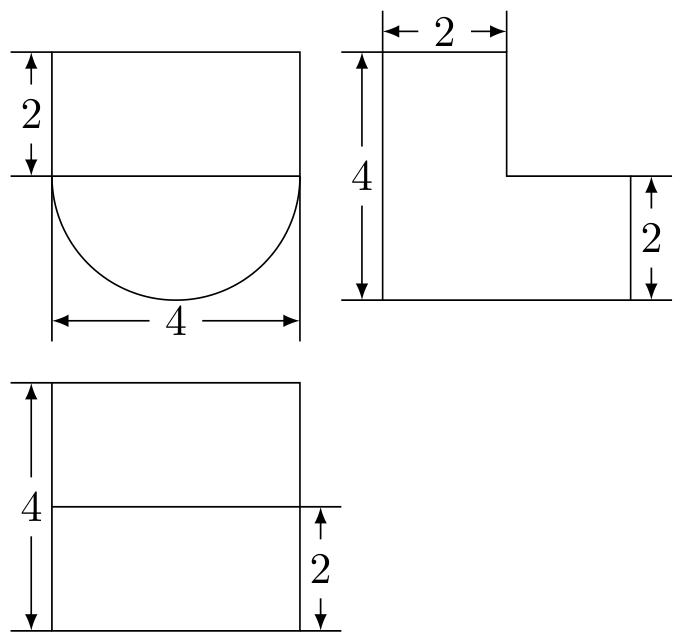
\includegraphics[width=6.8cm]{GaoKao/images/2013/new_curriculum_paper_1_liberal/q11_fig1.png}
\end{center}

        {\centering\begin{tabular*}{\linewidth}{@{}@{\extracolsep{\fill}}llll@{}}
          \text{A. }\(16 + 8\pi\)  &  \text{B. }\(8 + 8\pi\)  &  \text{C. }\(16 + 16\pi\)  &  \text{D. }\(8 + 16\pi\)
        \end{tabular*}\par}

        \item 已知函数 \(f(x) = \begin{cases}
-x^2 + 2x, & x \leqslant 0,\\
\ln (x + 1), & x > 0,
\end{cases} \) 若 \(|f(x)| \geqslant ax\)，则 \( a \) 的取值范围是（\quad）

        {\centering\begin{tabular*}{\linewidth}{@{}@{\extracolsep{\fill}}llll@{}}
          \text{A. }\(\left(-\infty,0\right]\)  &  \text{B. }\(\left(-\infty,1\right]\)  &  \text{C. }\(\left[-2,1\right]\)  &  \text{D. }\(\left[-2,0\right]\)
        \end{tabular*}\par}

    \end{enumerate}

\end{description}

\begin{description}

    \item[二、填空题]

    \begin{enumerate}[leftmargin=5pt]

      \addtocounter{enumi}{+12}

        \item 已知两个单位向量 \(\bm{a}\)，\(\bm{b}\) 的夹角为 \(60^{\circ}\)，\(\bm{c} = t\bm{a} + (1 - t)\bm{b}\)，若 \(\bm{b} \cdot \bm{c} = 0\)，则 \(t =\)\rule[-0.3ex]{3em}{0.4pt}.

        \item 设 \(x\)，\(y\) 满足约束条件 \(\begin{cases}
1 \leqslant x \leqslant 3,\\
-1 \leqslant x - y \leqslant 0,
\end{cases}\)，则 \(z = 2x - y\) 的最大值为\rule[-0.3ex]{3em}{0.4pt}.

        \item 已知 \(H\) 是球 \(O\) 的直径 \(AB\) 上一点，\(AH:HB = 1:2\)，\(AB \perp\) 平面 \(\alpha\)，\(H\) 为垂足，平面 \(\alpha\) 截球 \(O\) 所得截面的面积为 \(\pi\)，则球 \(O\) 的表面积为\rule[-0.3ex]{3em}{0.4pt}.

        \item 设当 \(x = \theta\) 时，函数 \(f(x) = \sin x - 2\cos x\) 取得最大值，则 \(\cos \theta =\)\rule[-0.3ex]{3em}{0.4pt}.

    \end{enumerate}

\end{description}

\begin{description}

    \item[三、解答题]

    \begin{enumerate}[leftmargin=5pt]

      \addtocounter{enumi}{+16}

        \item 已知等差数列 \(\{a_{n}\}\) 的前 \(n\) 项和 \(S_{n}\) 满足 \(S_{3} = 0\)，\(S_{5} = -5\).
\begin{enumerate}
\item 求 \( \{a_{n}\} \) 的通项公式；
\item 求数列 \(\left\{\frac{1}{a_{2n-1}a_{2n+1}}\right\}\) 的前 \(n\) 项和.
\end{enumerate}

        \item 为了比较两种治疗失眠症的药（分别称为 A 药，B 药）的疗效，随机地选取 \(20\) 位患者服用 A 药，\(20\) 位患者服用 B 药，这 \(40\) 位患者在服用一段时间后，记录他们日平均增加的睡眠时间（单位：\(\mathrm{h}\)）. 试验的观测结果如下：

服用 A 药的 \(20\) 位患者日平均增加的睡眠时间：

\(0.6\) \(1.2\) \(2.7\) \(1.5\) \(2.8\) \(1.8\) \(2.2\) \(2.3\) \(3.2\) \(3.5\)
\(2.5\) \(2.6\) \(1.2\) \(2.7\) \(1.5\) \(2.9\) \(3.0\) \(3.1\) \(2.3\) \(2.4\)

服用 B 药的 \(20\) 位患者日平均增加的睡眠时间：

\(3.2\) \(1.7\) \(1.9\) \(0.8\) \(0.9\) \(2.4\) \(1.2\) \(2.6\) \(1.3\) \(1.4\)
\(1.6\) \(0.5\) \(1.8\) \(0.6\) \(2.1\) \(1.1\) \(2.5\) \(1.2\) \(2.7\) \(0.5\)

\begin{enumerate}
\item 分别计算两组数据的平均数，从计算结果看，哪种药的疗效更好？
\item 根据两组数据完成下面茎叶图，从茎叶图看，哪种药的疗效更好？
\end{enumerate}

\begin{center}
\begin{tabular}{c|c|c}
A药 &  & B药 \\
\hline
\(6\) & \(0\) & \(5\) \(5\) \(6\) \(8\) \(9\) \\
\(8\) \(5\) \(5\) \(2\) \(2\) & \(1\) & \(1\) \(2\) \(2\) \(3\) \(4\) \(6\) \(7\) \(8\) \(9\) \\
\(9\) \(8\) \(7\) \(7\) \(6\) \(5\) \(4\) \(3\) \(3\) \(2\) & \(2\) & \(1\) \(4\) \(5\) \(6\) \(7\) \\
\(5\) \(2\) \(1\) \(0\) & \(3\) & \(2\)
\end{tabular}
\end{center}

        \item 如图，三棱柱 \(ABC - A_{1}B_{1}C_{1}\) 中，\(CA = CB\)，\(AB = AA_{1}\)，\(\angle BAA_{1} = 60^{\circ}\).

\begin{enumerate}
\item 证明：\(AB \perp A_{1}C\)
\item 若 \(AB = CB = 2\)，\(A_{1}C = \sqrt{6}\)，求三棱柱 \(ABC - A_{1}B_{1}C_{1}\) 的体积.
\end{enumerate}

\begin{center}
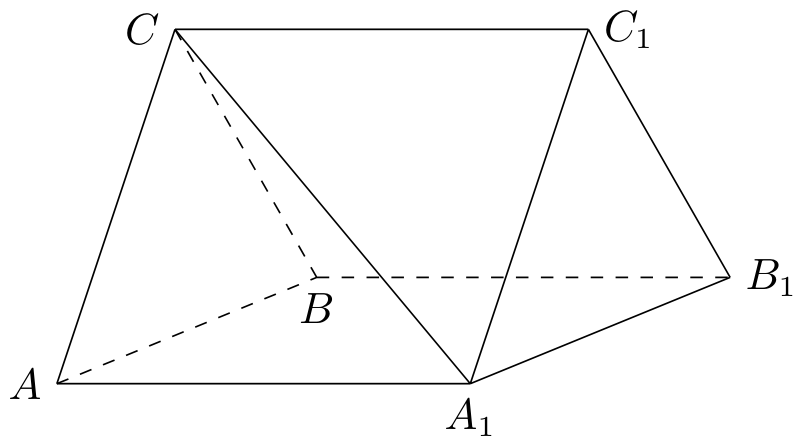
\includegraphics[width=10.6cm]{GaoKao/images/2013/new_curriculum_paper_1_liberal/q19_fig1.png}
\end{center}

        \item 已知函数 \(f(x) = {\mathrm{e}}^{x}(ax + b) - x^{2} - 4x\)，曲线 \(y = f(x)\) 在点 \((0,f(0))\) 处的切线方程为 \(y = 4x + 4\).
\begin{enumerate}
\item 求 \(a\)，\(b\) 的值；
\item 讨论 \( f(x) \) 的单调性，并求 \( f(x) \) 的极大值.
\end{enumerate}

        \item 已知圆 \(M: (x + 1)^2 + y^2 = 1\)，圆 \(N: (x - 1)^2 + y^2 = 9\)，动圆 \(P\) 与圆 \(M\) 外切并与圆 \(N\) 内切，圆心 \(P\) 的轨迹为曲线 \(C\).

\begin{enumerate}
\item 求 \(C\) 的方程；
\item \(l\) 是与圆 \(P\)，圆 \(M\) 都相切的一条直线，\(l\) 与曲线 \(C\) 交于 \(A\)，\(B\) 两点，当圆 \(P\) 的半径最长时，求 \(|AB|\).
\end{enumerate}

        \item 如图，直线 \(AB\) 为圆的切线，切点为 \(B\)，点 \(C\) 在圆上，\(\angle ABC\) 的角平分线 \(BE\) 交圆于点 \(E\)，\(DB\) 垂直 \(BE\) 交圆于 \(D\).

\begin{enumerate}
\item 证明： \(DB = DC\)；
\item 设圆的半径为 \(1\)，\(BC = \sqrt{3}\)，延长 \(CE\) 交 \(AB\) 于点 \(F\)，求 \(\triangle BCF\) 外接圆的半径.
\end{enumerate}

\begin{center}
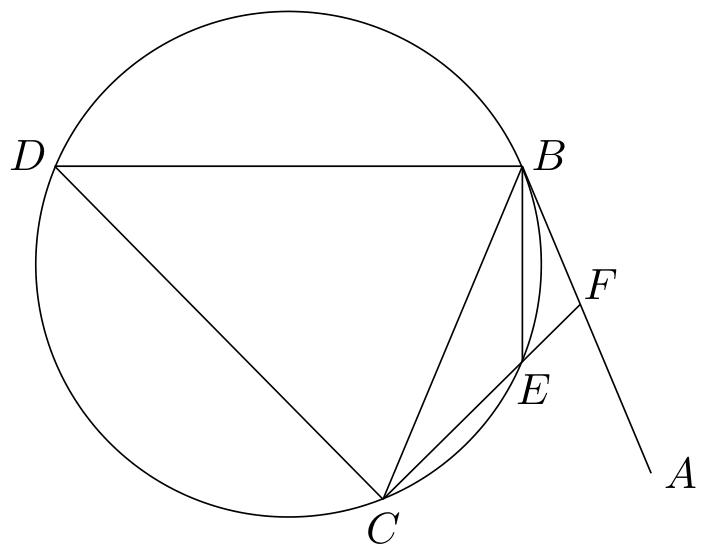
\includegraphics[width=8.5cm]{GaoKao/images/2013/new_curriculum_paper_1_liberal/q22_fig1.png}
\end{center}

        \item 已知曲线 \(C_1\) 的参数方程为 \(\begin{cases}
x = 4 + 5\cos t,\\
y = 5 + 5\sin t,
\end{cases}\)（\(t\) 为参数），以坐标原点为极点，\(x\) 轴的正半轴为极轴建立极坐标系，曲线 \(C_2\) 的极坐标方程为 \(\rho = 2\sin\theta\).
\begin{enumerate}
\item 把 \(C_1\) 的参数方程化为极坐标方程；
\item 求 \(C_{1}\) 与 \(C_{2}\) 交点的极坐标 \(\left(\rho \geqslant 0, 0 \leqslant \theta < 2\pi\right)\).
\end{enumerate}

        \item 已知函数 \( f(x) = |2x - 1| + |2x + a| \)，\( g(x) = x + 3 \).
\begin{enumerate}
\item 当 \(a = -2\) 时，求不等式 \(f(x) < g(x)\) 的解集；
\item 设 \(a > -1\)，且当 \(x \in \left[-\frac{a}{2}, \frac{1}{2}\right)\) 时，\(f(x) \leqslant g(x)\)，求 \(a\) 的取值范围.
\end{enumerate}

    \end{enumerate}

\end{description}


\subsection{2013年全国II卷（理）}\label{gk:2013年全国II卷（理）}

\begin{description}

    \item[一、选择题]

    \begin{enumerate}[leftmargin=5pt]

        \item 已知集合 \(M = \{x \mid (x - 1)^2 < 4, x \in \mathbb{R}\}\)，\(N = \{-1, 0, 1, 2, 3\}\)，则 \(M \cap N =\)（\quad）

        {\centering\begin{tabular*}{\linewidth}{@{}@{\extracolsep{\fill}}llll@{}}
          \text{A. }\(\{0, 1, 2\}\)  &  \text{B. }\(\{-1, 0, 1, 2\}\)  &  \text{C. }\(\{-1, 0, 2, 3\}\)  &  \text{D. }\(\{0, 1, 2, 3\}\)
        \end{tabular*}\par}

        \item 设复数 \(z\) 满足 \((1 - \i)z = 2\i\)，则 \(z =\)（\quad）

        {\centering\begin{tabular*}{\linewidth}{@{}@{\extracolsep{\fill}}llll@{}}
          \text{A. }\(-1 + \i\)  &  \text{B. }\(-1 - \i\)  &  \text{C. }\(1 + \i\)  &  \text{D. }\(1 - \i\)
        \end{tabular*}\par}

        \item 等比数列 \(\{a_n\}\) 的前 \(n\) 项和为 \(S_n\)，已知 \(S_3 = a_2 + 10a_1\)，\(a_5 = 9\)，则 \(a_1 =\)（\quad）

        {\centering\begin{tabular*}{\linewidth}{@{}@{\extracolsep{\fill}}llll@{}}
          \text{A. }\(\frac{1}{3}\)  &  \text{B. }\(-\frac{1}{3}\)  &  \text{C. }\(\frac{1}{9}\)  &  \text{D. }\(-\frac{1}{9}\)
        \end{tabular*}\par}

        \item 已知 \(m\)，\(n\) 为异面直线，\(m \perp\) 平面 \(\alpha\)，\(n \perp\) 平面 \(\beta\)，直线 \(l\) 满足 \(l \perp m\)，\(l \perp n\)，\(l \not\subset \alpha\)，\(l \not\subset \beta\)，则（\quad）

        {\centering\begin{tabular*}{\linewidth}{@{}@{\extracolsep{\fill}}llll@{}}
          \text{A. }\(\alpha \parallel \beta\) 且 \(l \parallel \alpha\)  &  \text{B. }\(\alpha \perp \beta\) 且 \(l \perp \beta\)  &  \text{C. }\(\alpha\) 与 \(\beta\) 相交，且交线垂直于 \(l\)  &  \text{D. }\(\alpha\) 与 \(\beta\) 相交，且交线平行于 \(l\)
        \end{tabular*}\par}

        \item 已知 \((1 + ax)(1 + x)^5\) 的展开式中 \(x^2\) 的系数为 5，则 \(a =\)（\quad）

        {\centering\begin{tabular*}{\linewidth}{@{}@{\extracolsep{\fill}}llll@{}}
          \text{A. }\(-4\)  &  \text{B. }\(-3\)  &  \text{C. }\(-2\)  &  \text{D. }\(-1\)
        \end{tabular*}\par}

        \item 执行如图的程序框图，如果输入的 \(N = 10\)，那么输出的 \(S =\)（\quad）

{
\begin{center}
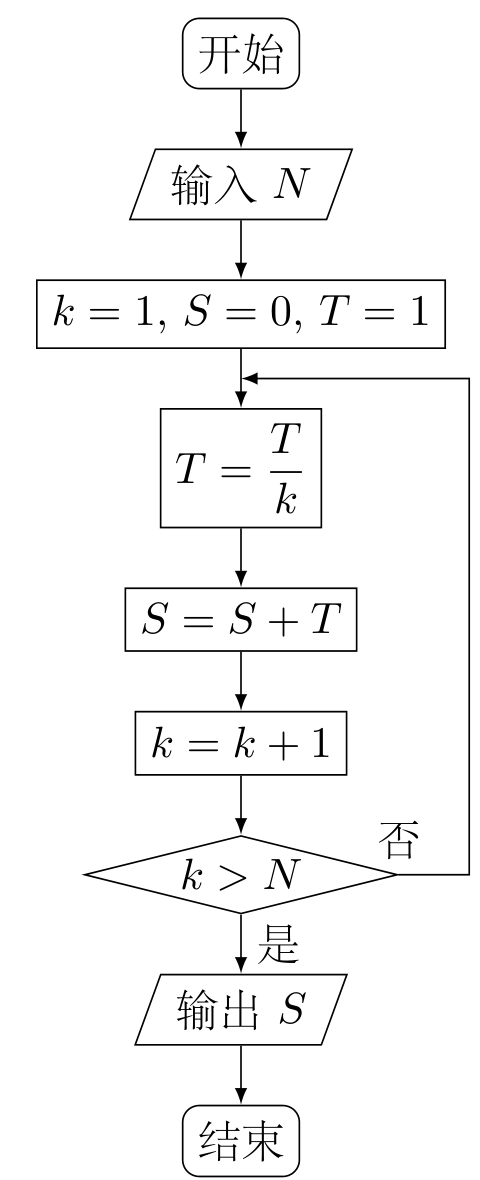
\includegraphics[width=0.38\linewidth]{GaoKao/images/2013/new_curriculum_paper_2_science/q6_fig1.png}
\end{center}
}

        {\centering\begin{tabular*}{\linewidth}{@{}@{\extracolsep{\fill}}llll@{}}
          \text{A. }\(1 + \frac{1}{2} + \frac{1}{3} + \dots + \frac{1}{10}\)  &  \text{B. }\(1 + \frac{1}{2!} + \frac{1}{3!} + \dots + \frac{1}{10!}\)  &  \text{C. }\(1 + \frac{1}{2} + \frac{1}{3} + \dots + \frac{1}{11}\)  &  \text{D. }\(1 + \frac{1}{2!} + \frac{1}{3!} + \dots + \frac{1}{11!}\)
        \end{tabular*}\par}

        \item 一个四面体的顶点在空间直角坐标系 \(O - xyz\) 中的坐标分别是 \((1, 0, 1)\)，\((1, 1, 0)\)，\((0, 1, 1)\)，\((0, 0, 0)\)，画该四面体三视图中的正视图时，以 \(zOx\) 平面为投影面，则得到正视图可以为（\quad）

        {\centering\begin{tabular*}{\linewidth}{@{}@{\extracolsep{\fill}}cccc@{}}
          \text{A. }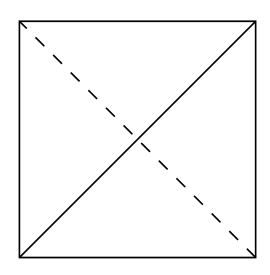
\includegraphics[width=0.15\paperwidth]{GaoKao/images/2013/new_curriculum_paper_2_science/q7_choice_a.png}  &  \text{B. }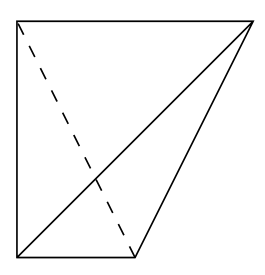
\includegraphics[width=0.15\paperwidth]{GaoKao/images/2013/new_curriculum_paper_2_science/q7_choice_b.png}  &  \text{C. }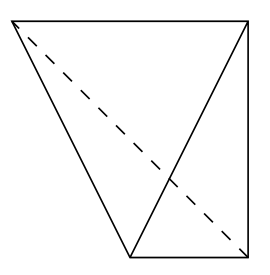
\includegraphics[width=0.15\paperwidth]{GaoKao/images/2013/new_curriculum_paper_2_science/q7_choice_c.png}  &  \text{D. }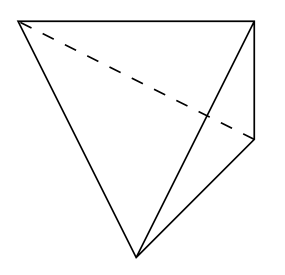
\includegraphics[width=0.15\paperwidth]{GaoKao/images/2013/new_curriculum_paper_2_science/q7_choice_d.png}
        \end{tabular*}\par}

        \item 设 \(a = \log_{3} 6\)，\(b = \log_{5} 10\)，\(c = \log_{7} 14\)，则（\quad）

        {\centering\begin{tabular*}{\linewidth}{@{}@{\extracolsep{\fill}}llll@{}}
          \text{A. }\(c > b > a\)  &  \text{B. }\(b > c > a\)  &  \text{C. }\(a > c > b\)  &  \text{D. }\(a > b > c\)
        \end{tabular*}\par}

        \item 已知 \(a > 0\)，\(x\)，\(y\) 满足约束条件 \(\begin{cases}
x \geqslant 1,\\
x + y \leqslant 3,\\
y \geqslant a (x - 3),
\end{cases}\) 若 \(z = 2x + y\) 的最小值为 1，则 \(a =\)（\quad）

        {\centering\begin{tabular*}{\linewidth}{@{}@{\extracolsep{\fill}}llll@{}}
          \text{A. }\(\frac{1}{4}\)  &  \text{B. }\(\frac{1}{2}\)  &  \text{C. }\(1\)  &  \text{D. }\(2\)
        \end{tabular*}\par}

        \item 已知函数 \(f(x) = x^3 + ax^2 + bx + c\)，下列结论中错误的是（\quad）

        {\centering\begin{tabular*}{\linewidth}{@{}@{\extracolsep{\fill}}llll@{}}
          \text{A. }\(\exists x_0 \in \mathbb{R}, f(x_0) = 0\)  &  \text{B. }函数 \(y = f(x)\) 的图象是中心对称图形  &  \text{C. }若 \(x_0\) 是 \(f(x)\) 的极小值点，则 \(f(x)\) 在区间 \((-\infty, x_0)\) 单调递减  &  \text{D. }若 \(x_0\) 是 \(f(x)\) 的极值点，则 \(f'(x_0) = 0\)
        \end{tabular*}\par}

        \item 设抛物线 \(C: y^2 = 2px\)（\(p > 0\)）的焦点为 \(F\)，点 \(M\) 在 \(C\) 上，\(|MF| = 5\). 若以 \(MF\) 为直径的圆过点 \((0,2)\)，则 \(C\) 的方程为（\quad）

        {\centering\begin{tabular*}{\linewidth}{@{}@{\extracolsep{\fill}}llll@{}}
          \text{A. }\(y^2 = 4x\) 或 \(y^2 = 8x\)  &  \text{B. }\(y^2 = 2x\) 或 \(y^2 = 8x\)  &  \text{C. }\(y^2 = 4x\) 或 \(y^2 = 16x\)  &  \text{D. }\(y^2 = 2x\) 或 \(y^2 = 16x\)
        \end{tabular*}\par}

        \item 已知点 \(A(-1, 0)\)，\(B(1, 0)\)，\(C(0, 1)\)，直线 \(y = ax + b\)（\(a > 0\)）将 \(\triangle ABC\) 分割为面积相等的两部分，则 \(b\) 的取值范围是（\quad）

        {\centering\begin{tabular*}{\linewidth}{@{}@{\extracolsep{\fill}}llll@{}}
          \text{A. }\((0, 1)\)  &  \text{B. }\(\left(1 - \frac{\sqrt{2}}{2}, \frac{1}{2}\right)\)  &  \text{C. }\(\left(1 - \frac{\sqrt{2}}{2}, \frac{1}{3}\right]\)  &  \text{D. }\(\left[\frac{1}{3}, \frac{1}{2}\right)\)
        \end{tabular*}\par}

    \end{enumerate}

\end{description}

\begin{description}

    \item[二、填空题]

    \begin{enumerate}[leftmargin=5pt]

      \addtocounter{enumi}{+12}

        \item 已知正方形 \(ABCD\) 的边长为 \(2\)，\(E\) 为 \(CD\) 的中点，则 \(\overrightarrow{AE} \cdot \overrightarrow{BD} =\)\rule[-0.3ex]{3em}{0.4pt}.

        \item 从 \(n\) 个正整数 \(1\)，\(2\)，\(\cdots\)，\(n\) 中任意取出两个不同的数，若取出的两数之和等于 5 的概率为 \(\frac{1}{14}\)，则 \(n =\)\rule[-0.3ex]{3em}{0.4pt}.

        \item 设 \(\theta\) 为第二象限角，若 \(\tan \left( \theta + \frac{\pi}{4} \right) = \frac{1}{2}\)，则 \(\sin \theta + \cos \theta =\)\rule[-0.3ex]{3em}{0.4pt}.

        \item 等差数列 \(\{a_n\}\) 的前 \(n\) 项和为 \(S_n\)，已知 \(S_{10} = 0\)，\(S_{15} = 25\)，则 \(nS_n\) 的最小值为\rule[-0.3ex]{3em}{0.4pt}.

    \end{enumerate}

\end{description}

\begin{description}

    \item[三、解答题]

    \begin{enumerate}[leftmargin=5pt]

      \addtocounter{enumi}{+16}

        \item \(\triangle ABC\) 的内角 \(A\)，\(B\)，\(C\) 的对边分别为 \(a\)，\(b\)，\(c\)，已知 \(a = b\cos C + c\sin B\).
\begin{enumerate}
\item 求 \(B\)；
\item 若 \(b = 2\)，求 \(\triangle ABC\) 面积的最大值.
\end{enumerate}

        \item 如图，直三棱柱 \(ABC - A_1B_1C_1\) 中，\(D\)，\(E\) 分别是 \(AB\)，\(BB_1\) 的中点，\(AA_1 = AC = CB = \frac{\sqrt{2}}{2}AB\).
\begin{enumerate}
\item 证明：\(BC_1 \parallel\) 平面 \(A_1CD\)；
\item 求二面角 \(D - A_1C - E\) 的正弦值.
\end{enumerate}

\begin{center}
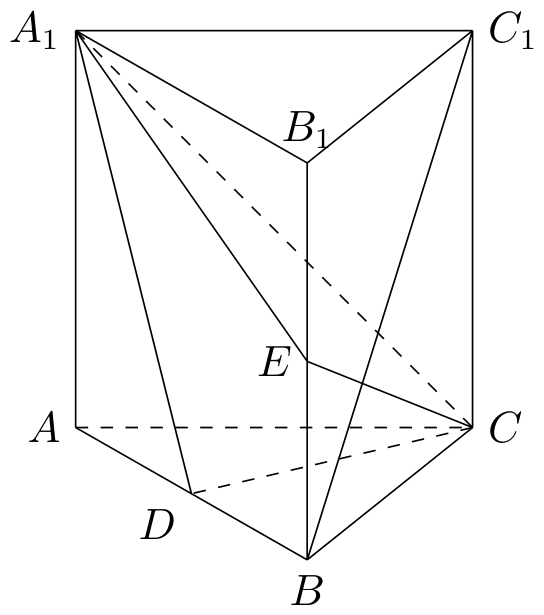
\includegraphics[width=5.3cm]{GaoKao/images/2013/new_curriculum_paper_2_science/q18_fig1.png}
\end{center}

        \item 经销商经销某种农产品，在一个销售季度内，每售出 \(1\mathrm{~t}\) 该产品获利润 \(500\text{ 元}\)，未售出的产品，每 \(1\mathrm{~t}\) 亏损 \(300\text{ 元}\). 根据历史资料，得到销售季度内市场需求量的频率分布直方图，如图所示. 经销商为下一个销售季度购进了 \(130\mathrm{~t}\) 该农产品. 以 \(X\)（单位：\(\mathrm{t}\)，\(100 \leqslant X \leqslant 150\)）表示下一个销售季度内的市场需求量，\(T\)（单位：\(\text{元}\)）表示下一个销售季度内经销该农产品的利润.

\begin{enumerate}
\item 将 \(T\) 表示为 \(X\) 的函数；
\item 根据直方图估计利润 \(T\) 不少于 57000 元的概率；
\item 在直方图的需求量分组中，以各组的区间中点值代表该组的各个值，需求量落入该区间的频率作为需求量取该区间中点值的概率（例如：若需求量 \(X \in [100, 110)\)，则取 \(X = 105\)，且 \(X = 105\) 的概率等于需求量落入 \([100, 110)\) 的频率），求 \(T\) 的数学期望.
\end{enumerate}

\begin{center}
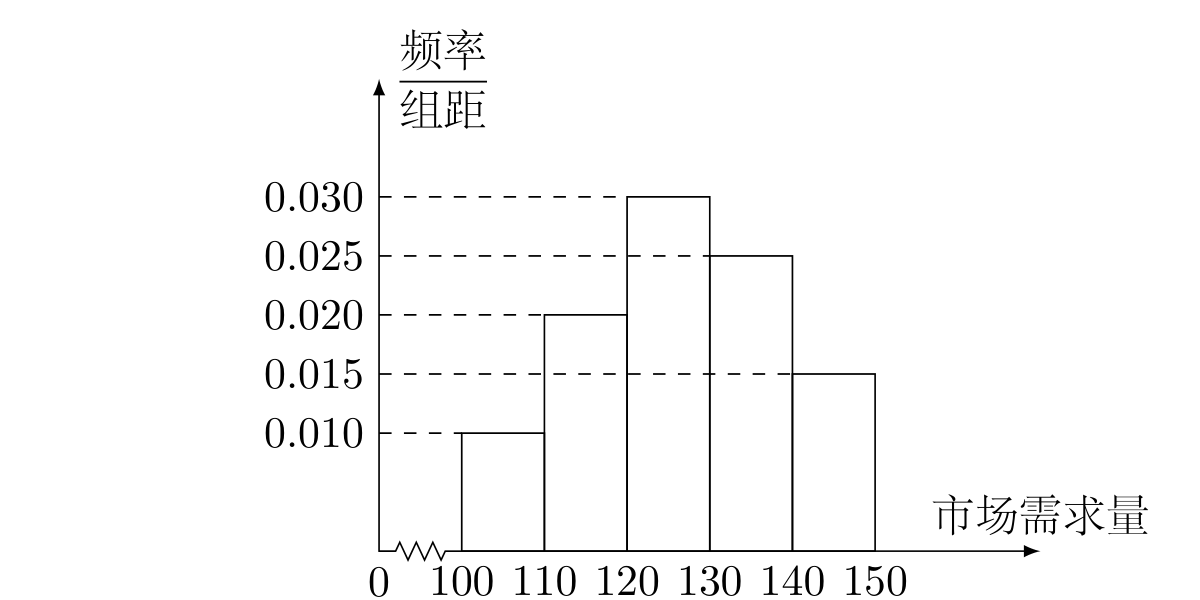
\includegraphics[width=0.42\linewidth]{GaoKao/images/2013/new_curriculum_paper_2_science/q19_fig1.png}
\end{center}

        \item 平面直角坐标系 \(xOy\) 中，过椭圆 \(M: \frac{x^2}{a^2} + \frac{y^2}{b^2} = 1\)（\(a > b > 0\)）右焦点的直线 \(x + y - \sqrt{3} = 0\) 交 \(M\) 于 \(A\)，\(B\) 两点，\(P\) 为 \(AB\) 的中点，且 \(OP\) 的斜率为 \(\frac{1}{2}\).

\begin{enumerate}
\item 求 \(M\) 的方程；
\item \(C\)，\(D\) 为 \(M\) 上两点，若四边形 \(ACBD\) 的对角线 \(CD \perp AB\)，求四边形 \(ACBD\) 面积的最大值.
\end{enumerate}

        \item 已知函数 \(f(x) = {\mathrm{e}}^{x} - \ln(x + m)\).

\begin{enumerate}
\item 设 \(x = 0\) 是 \(f(x)\) 的极值点，求 \(m\)，并讨论 \(f(x)\) 的单调性；
\item 当 \(m \leqslant 2\) 时，证明 \(f(x) > 0\).
\end{enumerate}

        \item 如图，\(CD\) 为 \(\triangle ABC\) 外接圆的切线，\(AB\) 的延长线交直线 \(CD\) 于点 \(D\)，\(E\)，\(F\) 分别为弦 \(AB\) 与弦 \(AC\) 上的点，且 \(BC \cdot AE = DC \cdot AF\)，\(B\)，\(E\)，\(F\)，\(C\) 四点共圆.

\begin{enumerate}
\item 证明：\(CA\) 是 \(\triangle ABC\) 外接圆的直径；
\item 若 \(DB = BE = EA\)，求过 \(B\)，\(E\)，\(F\)，\(C\) 四点的圆的面积与 \(\triangle ABC\) 外接圆面积的比值.
\end{enumerate}

\begin{center}
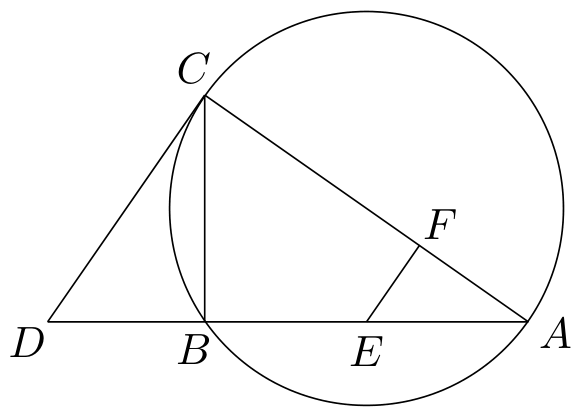
\includegraphics[width=7.0cm]{GaoKao/images/2013/new_curriculum_paper_2_science/q22_fig1.png}
\end{center}

        \item 已知动点 \(P\)，\(Q\) 都在曲线 \(C: \begin{cases}
x = 2\cos t,\\
y = 2\sin t,
\end{cases}\)（\(t\) 为参数）上，对应参数分别为 \(t = \alpha\) 与 \(t = 2\alpha\)（\(0 < \alpha < 2\pi\)），\(M\) 为 \(PQ\) 的中点.

\begin{enumerate}
\item 求 \(M\) 的轨迹的参数方程；
\item 将 \(M\) 到坐标原点的距离 \(d\) 表示为 \(\alpha\) 的函数，并判断 \(M\) 的轨迹是否过坐标原点.
\end{enumerate}

        \item 设 \(a\)，\(b\)，\(c\) 均为正数，且 \(a + b + c = 1\)，证明：

\begin{enumerate}
\item \(ab + bc + ca \leqslant \frac{1}{3}\)；
\item \(\frac{a^2}{b} + \frac{b^2}{c} + \frac{c^2}{a} \geqslant 1\).
\end{enumerate}

    \end{enumerate}

\end{description}


\subsection{2013年全国II卷（文）}\label{gk:2013年全国II卷（文）}

\begin{description}

    \item[一、选择题]

    \begin{enumerate}[leftmargin=5pt]

        \item 已知集合 \(M = \{x \mid -3 < x < 1\}\)，\(N = \{-3, -2, -1, 0, 1\}\)，则 \(M \cap N =\)（\quad）

        {\centering\begin{tabular*}{\linewidth}{@{}@{\extracolsep{\fill}}llll@{}}
          \text{A. }\( \{-2,-1,0,1\} \)  &  \text{B. }\( \{-3,-2,-1,0\} \)  &  \text{C. }\( \{-2,-1,0\} \)  &  \text{D. }\(\{-3, -2, -1\}\)
        \end{tabular*}\par}

        \item \(\left|\frac{2}{1 + \i}\right| =\)（\quad）

        {\centering\begin{tabular*}{\linewidth}{@{}@{\extracolsep{\fill}}llll@{}}
          \text{A. }\(2\sqrt{2}\)  &  \text{B. }\(2\)  &  \text{C. }\(\sqrt{2}\)  &  \text{D. }\(1\)
        \end{tabular*}\par}

        \item 设 \(x\)，\(y\) 满足约束条件 \(\begin{cases}
x - y + 1 \geqslant 0,\\
x + y - 1 \geqslant 0,\\
x \leqslant 3,
\end{cases}\) 则 \(z = 2x - 3y\) 的最小值是（\quad）

        {\centering\begin{tabular*}{\linewidth}{@{}@{\extracolsep{\fill}}llll@{}}
          \text{A. }\(-7\)  &  \text{B. }\(-6\)  &  \text{C. }\(-5\)  &  \text{D. }\(-3\)
        \end{tabular*}\par}

        \item \(\triangle ABC\) 的内角 \(A\)，\(B\)，\(C\) 的对边分别为 \(a\)，\(b\)，\(c\). 已知 \(b = 2\)，\(B = \frac{\pi}{6}\)，\(C = \frac{\pi}{4}\)，则 \(\triangle ABC\) 的面积为（\quad）

        {\centering\begin{tabular*}{\linewidth}{@{}@{\extracolsep{\fill}}llll@{}}
          \text{A. }\(2\sqrt{3} + 2\)  &  \text{B. }\(\sqrt{3} + 1\)  &  \text{C. }\(2\sqrt{3} - 2\)  &  \text{D. }\(\sqrt{3} - 1\)
        \end{tabular*}\par}

        \item 设椭圆 \(C: \frac{x^2}{a^2} + \frac{y^2}{b^2} = 1\)（\(a > b > 0\)）的左，右焦点分别为 \(F_1\)，\(F_2\)，\(P\) 是 \(C\) 上的点，\(PF_2 \perp F_1F_2\)，\(\angle PF_1F_2 = 30^\circ\)，则 \(C\) 的离心率为（\quad）

        {\centering\begin{tabular*}{\linewidth}{@{}@{\extracolsep{\fill}}llll@{}}
          \text{A. }\(\frac{\sqrt{3}}{6}\)  &  \text{B. }\(\frac{1}{3}\)  &  \text{C. }\(\frac{1}{2}\)  &  \text{D. }\(\frac{\sqrt{3}}{3}\)
        \end{tabular*}\par}

        \item 已知 \(\sin 2\alpha = \frac{2}{3}\)，则 \(\cos^2\left(\alpha + \frac{\pi}{4}\right) =\)（\quad）

        {\centering\begin{tabular*}{\linewidth}{@{}@{\extracolsep{\fill}}llll@{}}
          \text{A. }\(\frac{1}{6}\)  &  \text{B. }\(\frac{1}{3}\)  &  \text{C. }\(\frac{1}{2}\)  &  \text{D. }\(\frac{2}{3}\)
        \end{tabular*}\par}

        \item 执行如图的程序框图，如果输入的 \(N = 4\)，那么输出的 \(S =\)（\quad）

\begin{center}
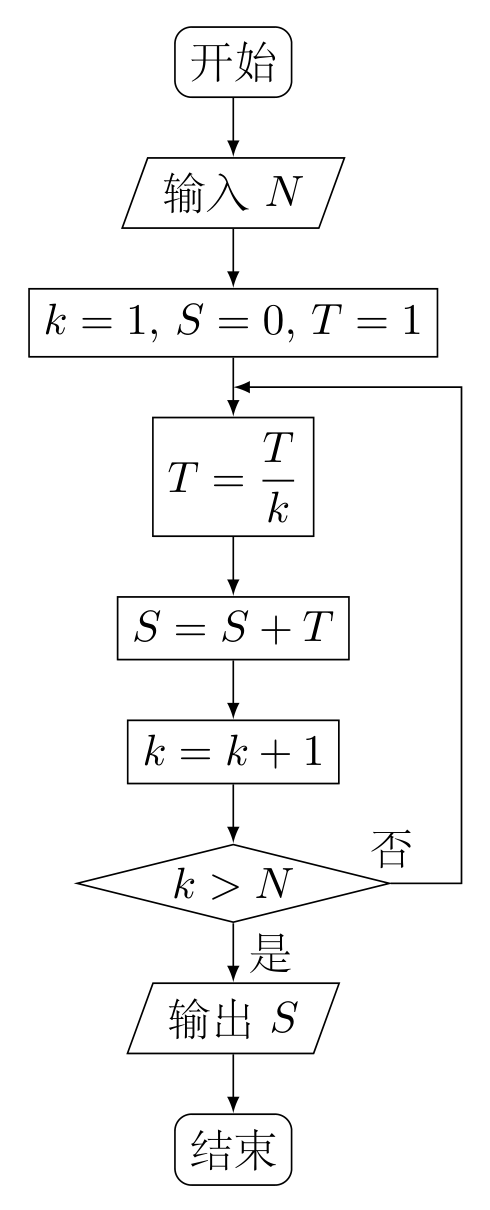
\includegraphics[width=0.32\linewidth]{GaoKao/images/2013/new_curriculum_paper_2_liberal/q7_fig1.png}
\end{center}

        {\centering\begin{tabular*}{\linewidth}{@{}@{\extracolsep{\fill}}llll@{}}
          \text{A. }\(1 + \frac{1}{2} +\frac{1}{3} +\frac{1}{4}\)  &  \text{B. }\(1 + \frac{1}{2} +\frac{1}{3\times 2} +\frac{1}{4\times 3\times 2}\)  &  \text{C. }\(1 + \frac{1}{2} +\frac{1}{3} +\frac{1}{4} +\frac{1}{5}\)  &  \text{D. }\(1 + \frac{1}{2} +\frac{1}{3\times 2} +\frac{1}{4\times 3\times 2} +\frac{1}{5\times 4\times 3\times 2}\)
        \end{tabular*}\par}

        \item 设 \(a = \log_{3} 2\)，\(b = \log_{5} 2\)，\(c = \log_{2} 3\)，则（\quad）

        {\centering\begin{tabular*}{\linewidth}{@{}@{\extracolsep{\fill}}llll@{}}
          \text{A. }\(a > c > b\)  &  \text{B. }\(b > c > a\)  &  \text{C. }\(c > b > a\)  &  \text{D. }\(c > a > b\)
        \end{tabular*}\par}

        \item 一个四面体的顶点在空间直角坐标系 \(O - xyz\) 中的坐标分别是 \( (1,0,1) \)， \( (1,1,0) \)， \( (0,1,1) \)， \( (0,0,0) \)，画该四面体三视图中的正视图时，以 \(zOx\) 平面为投影面，则得到正视图可以为（\quad）

        {\centering\begin{tabular*}{\linewidth}{@{}@{\extracolsep{\fill}}cccc@{}}
          \text{A. }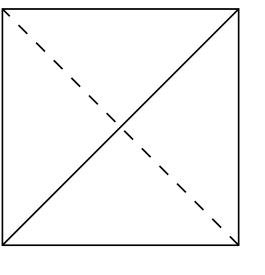
\includegraphics[width=0.15\paperwidth]{GaoKao/images/2013/new_curriculum_paper_2_liberal/q9_optA.png}  &  \text{B. }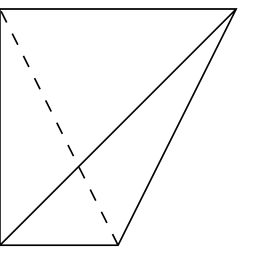
\includegraphics[width=0.15\paperwidth]{GaoKao/images/2013/new_curriculum_paper_2_liberal/q9_optB.png}  &  \text{C. }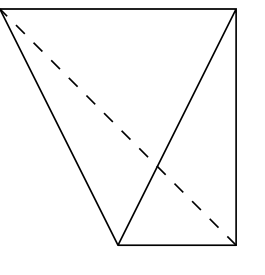
\includegraphics[width=0.15\paperwidth]{GaoKao/images/2013/new_curriculum_paper_2_liberal/q9_optC.png}  &  \text{D. }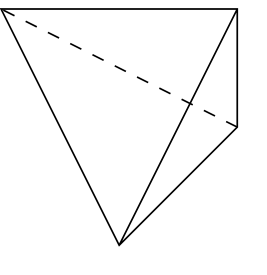
\includegraphics[width=0.15\paperwidth]{GaoKao/images/2013/new_curriculum_paper_2_liberal/q9_optD.png}
        \end{tabular*}\par}

        \item 设抛物线 \(C: y^{2} = 4x\) 的焦点为 \(F\)，直线 \(l\) 过 \(F\) 且与 \(C\) 交于 \(A\)，\(B\) 两点，若 \(|AF| = 3|BF|\)，则 \(l\) 的方程为（\quad）

        {\centering\begin{tabular*}{\linewidth}{@{}@{\extracolsep{\fill}}llll@{}}
          \text{A. }\( y = x - 1 \) 或 \( y = -x + 1 \)  &  \text{B. }\( y = \frac{\sqrt{3}}{3} (x - 1) \) 或 \( y = -\frac{\sqrt{3}}{3} (x - 1) \)  &  \text{C. }\( y = \sqrt{3} (x - 1) \) 或 \( y = -\sqrt{3} (x - 1) \)  &  \text{D. }\( y = \frac{\sqrt{2}}{2} (x - 1) \) 或 \( y = -\frac{\sqrt{2}}{2} (x - 1) \)
        \end{tabular*}\par}

        \item 已知函数 \( f(x) = x^{3} + ax^{2} + bx + c \)，下列结论中错误的是（\quad）

        {\centering\begin{tabular*}{\linewidth}{@{}@{\extracolsep{\fill}}llll@{}}
          \text{A. }\(\exists x_{0}\in \mathbb{R}, f(x_{0}) = 0\)  &  \text{B. }函数 \( y = f(x) \) 的图象是中心对称图形  &  \text{C. }若 \(x_0\) 是 \(f(x)\) 的极小值点，则 \(f(x)\) 在区间 \((- \infty, x_0)\) 单调递减  &  \text{D. }若 \(x_0\) 是 \(f(x)\) 的极值点，则 \(f'(x_0) = 0\)
        \end{tabular*}\par}

        \item 若存在正数 \(x\) 使 \(2^{x} (x - a) < 1\) 成立，则 \(a\) 的取值范围是（\quad）

        {\centering\begin{tabular*}{\linewidth}{@{}@{\extracolsep{\fill}}llll@{}}
          \text{A. }\((- \infty, + \infty)\)  &  \text{B. }\((-2, +\infty)\)  &  \text{C. }\((0, +\infty)\)  &  \text{D. }\((-1, +\infty)\)
        \end{tabular*}\par}

    \end{enumerate}

\end{description}

\begin{description}

    \item[二、填空题]

    \begin{enumerate}[leftmargin=5pt]

      \addtocounter{enumi}{+12}

        \item 从 \(1\)，\(2\)，\(3\)，\(4\)，\(5\) 中任意取出两个不同的数，其和为 \(5\) 的概率是\rule[-0.3ex]{3em}{0.4pt}.

        \item 已知正方形 \(ABCD\) 的边长为 \(2\)，\(E\) 为 \(CD\) 的中点，则 \(\overrightarrow{AE} \cdot \overrightarrow{BD} =\)\rule[-0.3ex]{3em}{0.4pt}.

        \item 已知正四棱锥 \(O - ABCD\) 的体积为 \(\frac{3\sqrt{2}}{2}\)，底面边长为 \(\sqrt{3}\)，则以 \(O\) 为球心，\(OA\) 为半径的球的表面积为\rule[-0.3ex]{3em}{0.4pt}.

        \item 函数 \( y = \cos (2x + \varphi) \) （\(- \pi \leqslant \varphi < \pi\)）的图象向右平移 \( \frac{\pi}{2} \) 个单位后，与函数 \( y = \sin \left(2x + \frac{\pi}{3}\right) \) 的图象重合，则 \( \varphi =\)\rule[-0.3ex]{3em}{0.4pt}.

    \end{enumerate}

\end{description}

\begin{description}

    \item[三、解答题]

    \begin{enumerate}[leftmargin=5pt]

      \addtocounter{enumi}{+16}

        \item 已知等差数列 \(\{a_{n}\}\) 的公差不为零，\(a_{1} = 25\)，且 \(a_{1}\)，\(a_{11}\)，\(a_{13}\) 成等比数列.
\begin{enumerate}
\item 求 \(\{a_{n}\}\) 的通项公式；
\item 求 \(a_{1} + a_{4} + a_{7} + \cdots + a_{3n - 2}\).
\end{enumerate}

        \item 如图，直三棱柱 \(ABC - A_{1}B_{1}C_{1}\) 中，\(D\)，\(E\) 分别是 \(AB\)，\(BB_{1}\) 的中点.

\begin{enumerate}
\item 证明： \(BC_{1} \parallel\) 平面 \(A_{1}CD\)；
\item 设 \(AA_{1} = AC = CB = 2\)，\(AB = 2\sqrt{2}\)，求三棱锥 \(C - A_{1}DE\) 的体积.
\end{enumerate}

\begin{center}
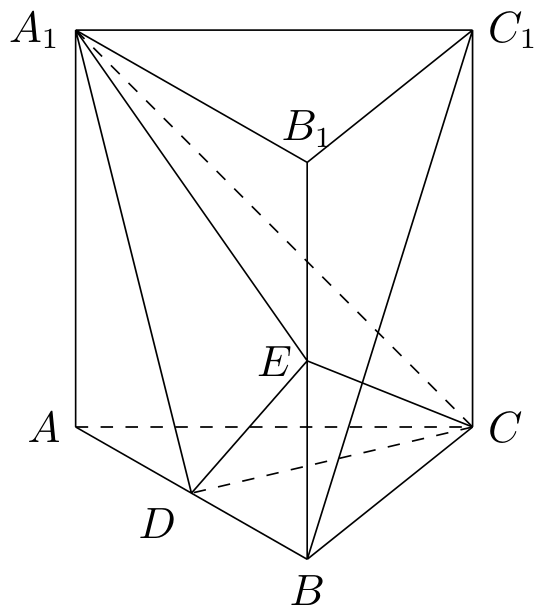
\includegraphics[width=5.6cm]{GaoKao/images/2013/new_curriculum_paper_2_liberal/q18_fig1.png}
\end{center}

        \item 经销商经销某种农产品，在一个销售季度内，每售出 \(1\mathrm{~t}\) 该产品获利润 \(500\text{ 元}\). 未售出的产品，每 \(1\mathrm{~t}\) 亏损 \(300\text{ 元}\). 根据历史资料，得到销售季度内市场需求量的频率分布直方图，如图所示. 经销商为下一个销售季度购进了 \(130\mathrm{~t}\) 该农产品. 以 \(X\)（单位：\(\mathrm{t}\)，\(100 \leqslant X \leqslant 150\)）表示下一个销售季度的市场需求量，\(T\)（单位：\(\text{元}\)）表示下一个销售季度内经销该农产品的利润.

\begin{enumerate}
\item 将 \(T\) 表示为 \(X\) 的函数；
\item 根据直方图估计利润 \(T\) 不少于 57000 元的概率.
\end{enumerate}

\begin{center}
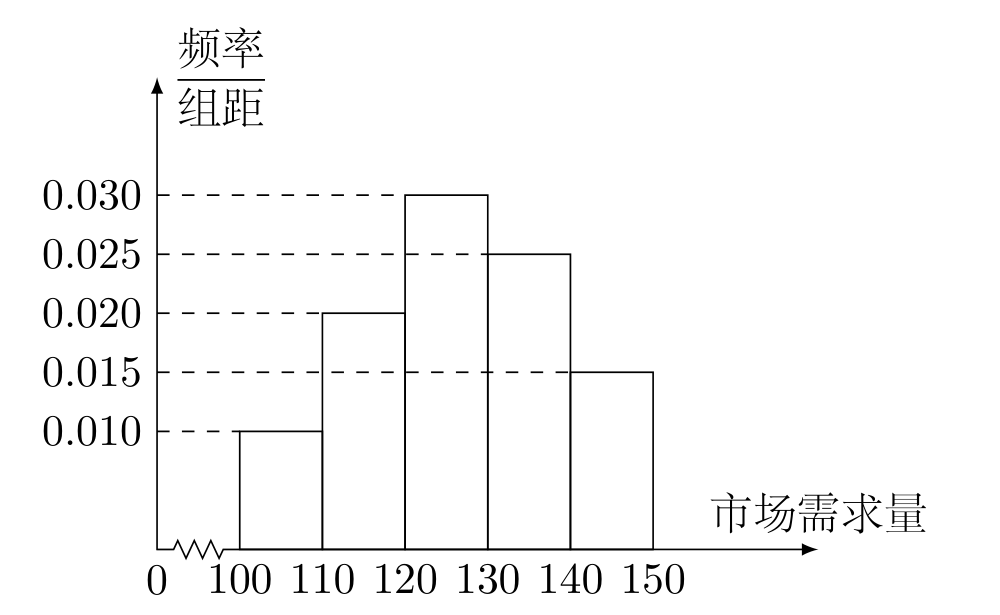
\includegraphics[width=0.46\linewidth]{GaoKao/images/2013/new_curriculum_paper_2_liberal/q19_fig1.png}
\end{center}

        \item 在平面直角坐标系 \(xOy\) 中，已知圆 \(P\) 在 \(x\) 轴上截得线段长为 \(2\sqrt{2}\)，在 \(y\) 轴上截得线段长为 \(2\sqrt{3}\).
\begin{enumerate}
\item 求圆心 \(P\) 的轨迹方程；
\item 若 \(P\) 点到直线 \(y = x\) 的距离为 \(\frac{\sqrt{3}}{2}\)，求圆 \(P\) 的方程.
\end{enumerate}

        \item 已知函数 \( f(x) = x^{2}{\mathrm{e}}^{-x} \).
\begin{enumerate}
\item 求 \( f(x) \) 的极小值和极大值；
\item 当曲线 \( y = f(x) \) 的切线 \( l \) 的斜率为负数时，求 \( l \) 在 \( x \) 轴上截距的取值范围.
\end{enumerate}

        \item 如图，\(CD\) 为 \(\triangle ABC\) 外接圆的切线，\(AB\) 的延长线交直线 \(CD\) 于点 \(D\)，\(E\)，\(F\) 分别为弦 \(AB\) 与弦 \(AC\) 上的点，且 \(BC \cdot AE = DC \cdot AF\)，\(B\)，\(E\)，\(F\)，\(C\) 四点共圆.

\begin{enumerate}
\item 证明： \(CA\) 是 \(\triangle ABC\) 外接圆的直径；
\item 若 \(DB = BE = EA\)，求过 \(B\)，\(E\)，\(F\)，\(C\) 四点的圆的面积与 \(\triangle ABC\) 外接圆面积的比值.
\end{enumerate}

\begin{center}
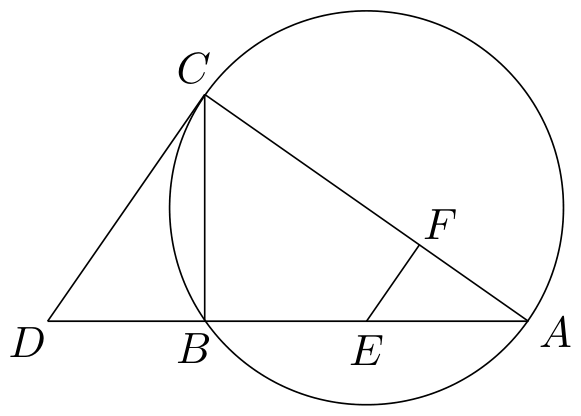
\includegraphics[width=7.0cm]{GaoKao/images/2013/new_curriculum_paper_2_liberal/q22_fig1.png}
\end{center}

        \item 已知动点 \(P\)，\(Q\) 都在曲线 \(C: \begin{cases}
x = 2\cos t,\\
y = 2\sin t,
\end{cases}\)（\(t\) 为参数）上，对应参数分别为 \(t = \alpha\) 与 \(t = 2\alpha\)（\(0 < \alpha < 2\pi\)），\(M\) 为 \(PQ\) 的中点.
\begin{enumerate}
\item 求 \(M\) 的轨迹的参数方程；
\item 将 \(M\) 到坐标原点的距离 \(d\) 表示为 \(\alpha\) 的函数，并判断 \(M\) 的轨迹是否过坐标原点.
\end{enumerate}

        \item 设 \(a\)，\(b\)，\(c\) 均为正数，且 \(a + b + c = 1\)，证明：
\begin{enumerate}
\item \(ab + bc + ca \leqslant \frac{1}{3}\)；
\item \(\frac{a^2}{b} + \frac{b^2}{c} + \frac{c^2}{a} \geqslant 1\).
\end{enumerate}

    \end{enumerate}

\end{description}


\subsection{2013年安徽卷（理）}\label{gk:2013年安徽卷（理）}

\begin{description}

    \item[一、选择题]

    \begin{enumerate}[leftmargin=5pt]

        \item 设 \(\i\) 是虚数单位，\(\overline{z}\) 是复数 \(z\) 的共轭复数，若 \(z \cdot \overline{z}\i + 2 = 2z\)，则 \(z =\)（\quad）

        {\centering\begin{tabular*}{\linewidth}{@{}@{\extracolsep{\fill}}llll@{}}
          \text{A. }\(1 + \i\)  &  \text{B. }\(1 - \i\)  &  \text{C. }\(-1 + \i\)  &  \text{D. }\(-1 - \i\)
        \end{tabular*}\par}

        \item 如图所示，程序框图（算法流程图）的输出结果是（\quad）

\begin{center}
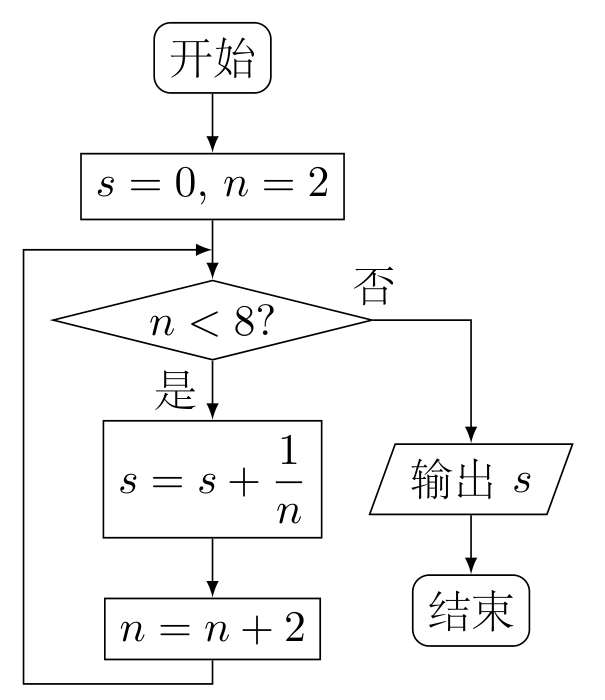
\includegraphics[width=0.40\linewidth]{GaoKao/images/2013/anhui_science/q2_fig1.png}
\end{center}

        {\centering\begin{tabular*}{\linewidth}{@{}@{\extracolsep{\fill}}llll@{}}
          \text{A. }\(\frac{1}{6}\)  &  \text{B. }\(\frac{25}{24}\)  &  \text{C. }\(\frac{3}{4}\)  &  \text{D. }\(\frac{11}{12}\)
        \end{tabular*}\par}

        \item 在下列命题中，不是公理的是（\quad）

        {\centering\begin{tabular*}{\linewidth}{@{}@{\extracolsep{\fill}}llll@{}}
          \text{A. }平行于同一个平面的两个平面相互平行  &  \text{B. }过不在同一条直线上的三点，有且只有一个平面  &  \text{C. }如果一条直线上的两点在一个平面内，那么这条直线上所有的点都在此平面内  &  \text{D. }如果两个不重合的平面有一个公共点，那么它们有且只有一条过该点的公共直线
        \end{tabular*}\par}

        \item “\(a \leqslant 0\)”是“函数 \(f(x) = |(ax - 1)x|\) 在区间 \((0, +\infty)\) 内单调递增”的（\quad）

        {\centering\begin{tabular*}{\linewidth}{@{}@{\extracolsep{\fill}}llll@{}}
          \text{A. }充分不必要条件  &  \text{B. }必要不充分条件  &  \text{C. }充分必要条件  &  \text{D. }既不充分也不必要条件
        \end{tabular*}\par}

        \item 某班级有 50 名学生，其中有 30 名男生和 20 名女生，随机询问了该班五名男生和五名女生在某次数学测验中的成绩，五名男生的成绩分别为 86，94，88，92，90. 五名女生的成绩分别为 88，93，93，88，93. 下列说法一定正确的是（\quad）

        {\centering\begin{tabular*}{\linewidth}{@{}@{\extracolsep{\fill}}llll@{}}
          \text{A. }这种抽样方法是一种分层抽样  &  \text{B. }这种抽样方法是一种系统抽样  &  \text{C. }这五名男生成绩的方差大于这五名女生成绩的方差  &  \text{D. }该班男生成绩的平均数小于该班女生成绩的平均数
        \end{tabular*}\par}

        \item 已知一元二次不等式 \( f(x) < 0 \) 的解集为 \( \left\{x \mid x < -1 \text{\ 或\ } x > \frac{1}{2}\right\} \)，则 \( f(10^x) > 0 \) 的解集为（\quad）

        {\centering\begin{tabular*}{\linewidth}{@{}@{\extracolsep{\fill}}llll@{}}
          \text{A. }\(\{x \mid x < -1 \text{\ 或\ } x > -\lg 2\}\)  &  \text{B. }\(\{x \mid -1 < x < -\lg 2\}\)  &  \text{C. }\(\{x \mid x > -\lg 2\}\)  &  \text{D. }\(\{x \mid x < -\lg 2\}\)
        \end{tabular*}\par}

        \item 在极坐标系中，圆 \(\rho = 2\cos \theta\) 的垂直于极轴的两条切线方程分别为（\quad）

        {\centering\begin{tabular*}{\linewidth}{@{}@{\extracolsep{\fill}}llll@{}}
          \text{A. }\(\theta = 0\)（\(\rho \in \mathbb{R}\)）和 \(\rho \cos \theta = 2\)  &  \text{B. }\(\theta = \frac{\pi}{2}\)（\(\rho \in \mathbb{R}\)）和 \(\rho \cos \theta = 2\)  &  \text{C. }\(\theta = \frac{\pi}{2}\)（\(\rho \in \mathbb{R}\)）和 \(\rho \cos \theta = 1\)  &  \text{D. }\(\theta = 0\)（\(\rho \in \mathbb{R}\)）和 \(\rho \cos \theta = 1\)
        \end{tabular*}\par}

        \item 函数 \( y = f(x) \) 的图象如图所示，在区间 \([a, b]\) 上可找到 \( n (n \geqslant 2) \) 个不同的数 \(x_1\)，\(x_2\)，\(\cdots\)，\(x_n\)，使得 \( \frac{f(x_1)}{x_1} = \frac{f(x_2)}{x_2} = \cdots = \frac{f(x_n)}{x_n} \)，则 \( n \) 的取值范围为（\quad）

\begin{center}
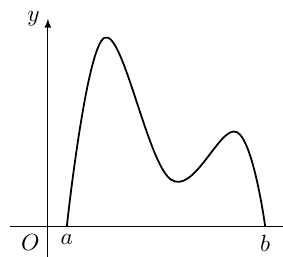
\includegraphics[width=5.9cm]{GaoKao/images/2013/anhui_science/q8_fig1.png}
\end{center}

        {\centering\begin{tabular*}{\linewidth}{@{}@{\extracolsep{\fill}}llll@{}}
          \text{A. }\( \{2, 3\} \)  &  \text{B. }\( \{2, 3, 4\} \)  &  \text{C. }\( \{3, 4\} \)  &  \text{D. }\( \{3, 4, 5\} \)
        \end{tabular*}\par}

        \item 在平面直角坐标系中， \(O\) 是坐标原点，两定点 \(A\)，\(B\) 满足 \(\left|\overrightarrow{OA}\right| = \left|\overrightarrow{OB}\right| = \overrightarrow{OA} \cdot \overrightarrow{OB} = 2\)，则点集 \(\left\{P \mid \overrightarrow{OP} = \lambda \overrightarrow{OA} + \mu \overrightarrow{OB}, |\lambda| + |\mu| \leqslant 1, \lambda, \mu \in \mathbb{R}\right\}\) 所表示的区域的面积是（\quad）

        {\centering\begin{tabular*}{\linewidth}{@{}@{\extracolsep{\fill}}llll@{}}
          \text{A. }\(2\sqrt{2}\)  &  \text{B. }\(2\sqrt{3}\)  &  \text{C. }\(4\sqrt{2}\)  &  \text{D. }\(4\sqrt{3}\)
        \end{tabular*}\par}

        \item 若函数 \( f(x) = x^3 + ax^2 + bx + c \) 有极值点 \(x_1\)，\(x_2\)，且 \( f(x_1) = x_1 \)，则关于 \( x \) 的方程 \( 3(f(x))^2 + 2af(x) + b = 0 \) 的不同实数根个数是（\quad）

        {\centering\begin{tabular*}{\linewidth}{@{}@{\extracolsep{\fill}}llll@{}}
          \text{A. }3  &  \text{B. }4  &  \text{C. }5  &  \text{D. }6
        \end{tabular*}\par}

    \end{enumerate}

\end{description}

\begin{description}

    \item[二、填空题]

    \begin{enumerate}[leftmargin=5pt]

      \addtocounter{enumi}{+10}

        \item 若 \(\left(x + \frac{a}{\sqrt[3]{x}}\right)^8\) 的展开式中 \(x^4\) 的系数为7，则实数 \(a = \)\rule[-0.3ex]{3em}{0.4pt}.

        \item 设 \(\triangle ABC\) 的内角 \(A\)，\(B\)，\(C\) 所对边的长分别为 \(a\)，\(b\)，\(c\). 若 \(b + c = 2a\)，\(3\sin A = 5\sin B\)，则角 \(C = \)\rule[-0.3ex]{3em}{0.4pt}.

        \item 已知直线 \( y = a \) 交抛物线 \( y = x^2 \) 于 \(A\)，\(B\) 两点，若该抛物线上存在点 \(C\)，使得 \( \angle ACB \) 为直角，则 \( a \) 的取值范围为\rule[-0.3ex]{3em}{0.4pt}.

        \item 如图，互不相同的点 \(A_{1}\)，\(A_{2}\)，\(\cdots\)，\(A_{n}\)，\(\cdots\) 和 \(B_{1}\)，\(B_{2}\)，\(\cdots\)，\(B_{n}\)，\(\cdots\) 分别在角 \(O\) 的两条边上. 所有 \(A_{n}B_{n}\) 相互平行，且所有梯形 \(A_{n}B_{n}B_{n+1}A_{n+1}\) 的面积均相等. 设 \(OA_{n} = a_{n}\). 若 \(a_{1} = 1\)，\(a_{2} = 2\)，则数列 \(\{a_{n}\}\) 的通项公式是\rule[-0.3ex]{3em}{0.4pt}.

\begin{center}
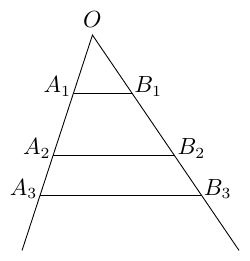
\includegraphics[width=5.2cm]{GaoKao/images/2013/anhui_science/q14_fig1.png}
\end{center}

        \item 如图，正方体 \(ABCD - A_{1}B_{1}C_{1}D_{1}\) 的棱长为 \(1\)，\(P\) 为 \(BC\) 中点，\(Q\) 为线段 \(CC_{1}\) 上的动点，过 \(A\)，\(P\)，\(Q\) 的平面截该正方体所得的截面记为 \(S\)，则下列命题正确的是\rule[-0.3ex]{3em}{0.4pt}.（写出所有正确命题的编号）

\begin{center}
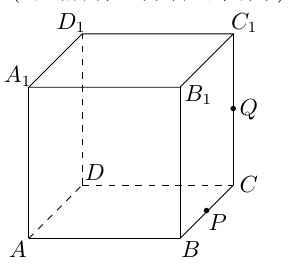
\includegraphics[width=5.6cm]{GaoKao/images/2013/anhui_science/q15_fig1.png}
\end{center}

\begin{enumerate}
\item 当 \(0 < CQ < \frac{1}{2}\) 时，\(S\) 为四边形；
    \item 当 \(CQ = \frac{1}{2}\) 时，\(S\) 为等腰梯形；
\item 当 \(CQ = \frac{3}{4}\) 时，\(S\) 与 \(C_{1}D_{1}\) 交点 \(R\) 满足 \(C_{1}R = \frac{1}{3}\)；
    \item 当 \(\frac{3}{4} < CQ < 1\) 时，\(S\) 为六边形；
\item 当 \(CQ = 1\) 时，\(S\) 的面积为 \(\frac{\sqrt{6}}{2}\).
\end{enumerate}

    \end{enumerate}

\end{description}

\begin{description}

    \item[三、解答题]

    \begin{enumerate}[leftmargin=5pt]

      \addtocounter{enumi}{+15}

        \item 已知函数 \(f(x) = 4\cos \omega x \cdot \sin \left( \omega x + \frac{\pi}{4} \right)\)（\(\omega > 0\)）的最小正周期为 \( \pi \).
\begin{enumerate}
\item 求 \( \omega \) 的值；
\item 讨论 \(f(x)\) 在区间 \(\left[0, \frac{\pi}{2}\right]\) 上的单调性.
\end{enumerate}

        \item 设函数 \( f(x) = ax - (1 + a^2)x^2 \)，其中 \(a > 0\)，区间 \( I = \{x \mid f(x) > 0\} \).
\begin{enumerate}
\item 求 \(I\) 的长度（注：区间 \((\alpha, \beta)\) 的长度定义为 \(\beta - \alpha\)）；
\item 给定常数 \(k \in (0,1)\)，当 \(1 - k \leqslant a \leqslant 1 + k\) 时，求 \(I\) 长度的最小值.
\end{enumerate}

        \item 设椭圆 \(E: \frac{x^2}{a^2} + \frac{y^2}{1-a^2} = 1\) 的焦点在 \(x\) 轴上.
\begin{enumerate}
\item 若椭圆 \(E\) 的焦距为 \(1\)，求椭圆 \(E\) 的方程；
\item 设 \(F_{1}\)，\(F_{2}\) 分别是椭圆 \(E\) 的左，右焦点，\(P\) 为椭圆 \(E\) 上第一象限内的点. 直线 \(F_{2}P\) 交 \(y\) 轴于点 \(Q\)，并且 \(F_{1}P \perp F_{1}Q\)，证明：当 \(a\) 变化时，点 \(P\) 在某定直线上.
\end{enumerate}

        \item 如图，圆锥顶点为 \(P\). 底面圆心为 \(O\)，其母线与底面所成的角为 \(22.5^{\circ}\). \(AB\) 和 \(CD\) 是底面圆 \(O\) 上的两条平行的弦，轴 \(OP\) 与平面 \(PCD\) 所成的角为 \(60^{\circ}\).

\begin{enumerate}
\item 证明：平面 \(PAB\) 与平面 \(PCD\) 的交线平行于底面；
\item 求 \( \cos\angle COD \).
\end{enumerate}

\begin{center}
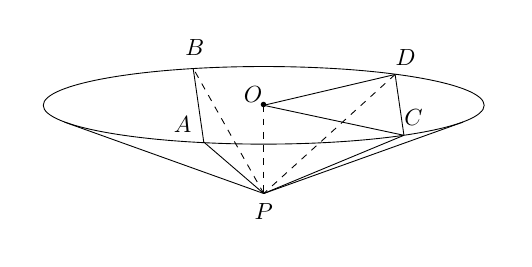
\includegraphics[width=12.0cm]{GaoKao/images/2013/anhui_science/q19_fig1.png}
\end{center}

        \item 设函数 \( f_{n}(x) = -1 + x + \frac{x^{2}}{2^{2}} + \frac{x^{3}}{3^{2}} + \cdots + \frac{x^{n}}{n^{2}}  \) （\(x \in \mathbb{R}, n \in \mathbb{N}^{*}\)）. 证明：
\begin{enumerate}
\item 对每个 \(n \in \mathbb{N}^*\)，存在唯一的 \(x_n \in \left[\frac{2}{3}, 1\right]\)，满足 \(f_n(x_n) = 0\)；
\item 对任意 \(p \in \mathbb{N}^*\)，由上一问中 \(x_n\) 构成的数列 \(\{x_n\}\) 满足 \(0 < x_n - x_{n+p} < \frac{1}{n}\).
\end{enumerate}

        \item 某高校数学系计划在周六和周日各举行一次主题不同的心理测试活动. 分别由李老师和张老师负责，已知该系共有 \(n\) 位学生，每次活动均需该系 \(k\) 位学生参加（\(n\) 和 \(k\) 都是固定的正整数）. 假设李老师和张老师分别将各自活动通知的信息独立，随机地发给该系 \(k\) 位学生，且所发信息都能收到. 记该系收到李老师或张老师所发活动通知信息的学生人数为 \(X\).
\begin{enumerate}
\item 求该系学生甲收到李老师或张老师所发活动通知信息的概率；
\item 求使 \(P(X = m)\) 取得最大值的整数 \(m\).
\end{enumerate}

    \end{enumerate}

\end{description}


\subsection{2013年安徽卷（文）}\label{gk:2013年安徽卷（文）}

\begin{description}

    \item[一、选择题]

    \begin{enumerate}[leftmargin=5pt]

        \item 设 \(i\) 是虚数单位，若复数 \(a - \frac{10}{3 - \i}\) （\(a \in \mathbb{R}\)） 是纯虚数，则 \(a\) 的值为（\quad）

        {\centering\begin{tabular*}{\linewidth}{@{}@{\extracolsep{\fill}}llll@{}}
          \text{A. }\(-3\)  &  \text{B. }\(-1\)  &  \text{C. }\(1\)  &  \text{D. }\(3\)
        \end{tabular*}\par}

        \item 已知 \(A = \{x \mid x + 1 > 0\}\)，\(B = \{-2, -1, 0, 1\}\)，则 \(\left(\complement_{\mathbb{R}} A\right) \cap B =\)（\quad）

        {\centering\begin{tabular*}{\linewidth}{@{}@{\extracolsep{\fill}}llll@{}}
          \text{A. }\(\{-2, -1\}\)  &  \text{B. }\(\{-2\}\)  &  \text{C. }\(\{-1, 0, 1\}\)  &  \text{D. }\(\{0, 1\}\)
        \end{tabular*}\par}

        \item 如图所示，程序框图 （算法流程图） 的输出结果是（\quad）

\begin{center}
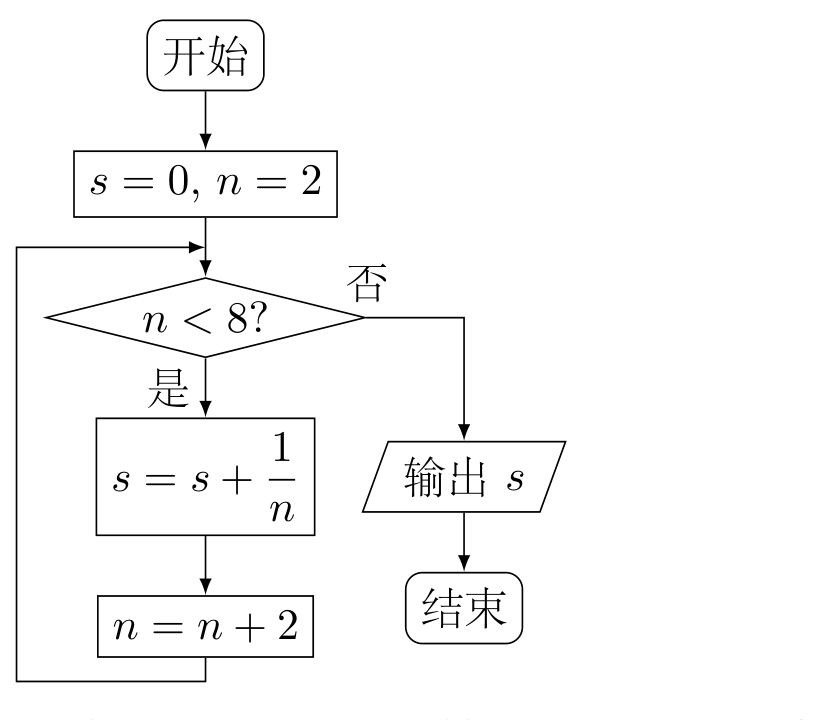
\includegraphics[width=0.40\linewidth]{GaoKao/images/2013/anhui_liberal/q3_fig1.png}
\end{center}

        {\centering\begin{tabular*}{\linewidth}{@{}@{\extracolsep{\fill}}llll@{}}
          \text{A. }\( \frac{3}{4} \)  &  \text{B. }\( \frac{1}{6} \)  &  \text{C. }\( \frac{11}{12} \)  &  \text{D. }\( \frac{25}{24} \)
        \end{tabular*}\par}

        \item “\((2x - 1)x = 0\)”是“\(x = 0\)”的（\quad）

        {\centering\begin{tabular*}{\linewidth}{@{}@{\extracolsep{\fill}}llll@{}}
          \text{A. }充分不必要条件  &  \text{B. }必要不充分条件  &  \text{C. }充分必要条件  &  \text{D. }既不充分也不必要条件
        \end{tabular*}\par}

        \item 若某公司从五位大学毕业生甲，乙，丙，丁，戊中录用三人，这五人被录用的机会均等，则甲或乙被录用的概率为（\quad）

        {\centering\begin{tabular*}{\linewidth}{@{}@{\extracolsep{\fill}}llll@{}}
          \text{A. }\( \frac{2}{3} \)  &  \text{B. }\( \frac{2}{5} \)  &  \text{C. }\( \frac{3}{5} \)  &  \text{D. }\( \frac{9}{10} \)
        \end{tabular*}\par}

        \item 直线 \(x + 2y - 5 + \sqrt{5} = 0\) 被圆 \(x^{2} + y^{2} - 2x - 4y = 0\) 截得的弦长为（\quad）

        {\centering\begin{tabular*}{\linewidth}{@{}@{\extracolsep{\fill}}llll@{}}
          \text{A. }\(1\)  &  \text{B. }\(2\)  &  \text{C. }\(4\)  &  \text{D. }\( 4\sqrt{6} \)
        \end{tabular*}\par}

        \item 设 \(S_{n}\) 为等差数列 \(\{a_{n}\}\) 的前 \(n\) 项和，\(S_{8} = 4a_{3}\)，\(a_{7} = -2\)，则 \(a_{9} =\)（\quad）

        {\centering\begin{tabular*}{\linewidth}{@{}@{\extracolsep{\fill}}llll@{}}
          \text{A. }\(-6\)  &  \text{B. }\(-4\)  &  \text{C. }\(-2\)  &  \text{D. }\(2\)
        \end{tabular*}\par}

        \item 函数 \( y = f(x) \) 的图象如图所示，在区间 \([a, b]\) 上可找到 \( n  \) （\(n \geqslant 2\)）个不同的数 \(x_1\)，\(x_2\)，\(\cdots\)，\(x_n\)，使得 \( \frac{f(x_1)}{x_1} = \frac{f(x_2)}{x_2} = \cdots = \frac{f(x_n)}{x_n} \)，则 \( n \) 的取值范围为（\quad）

\begin{center}
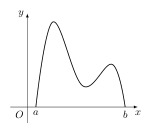
\includegraphics[width=7.0cm]{GaoKao/images/2013/anhui_liberal/q8_fig1.png}
\end{center}

        {\centering\begin{tabular*}{\linewidth}{@{}@{\extracolsep{\fill}}llll@{}}
          \text{A. }\(\{2, 3\}\)  &  \text{B. }\(\{2, 3, 4\}\)  &  \text{C. }\(\{3, 4\}\)  &  \text{D. }\(\{3, 4, 5\}\)
        \end{tabular*}\par}

        \item 设 \(\triangle ABC\) 的内角 \(A\)，\(B\)，\(C\) 所对边的长分别为 \(a\)，\(b\)，\(c\)，若 \(b + c = 2a\)，\(3\sin A = 5\sin B\)，则角 \(C =\)（\quad）

        {\centering\begin{tabular*}{\linewidth}{@{}@{\extracolsep{\fill}}llll@{}}
          \text{A. }\( \frac{\pi}{3} \)  &  \text{B. }\( \frac{2\pi}{3} \)  &  \text{C. }\( \frac{3\pi}{4} \)  &  \text{D. }\(\frac{5\pi}{6}\)
        \end{tabular*}\par}

        \item 已知函数 \( f(x) = x^3 + ax^2 + bx + c \) 有两个极值点 \(x_1\)，\(x_2\)，若 \( f(x_1) = x_1 < x_2 \)，则关于 \( x \) 的方程 \( 3(f(x))^2 + 2af(x) + b = 0 \) 的不同实根个数为（\quad）

        {\centering\begin{tabular*}{\linewidth}{@{}@{\extracolsep{\fill}}llll@{}}
          \text{A. }\(3\)  &  \text{B. }\(4\)  &  \text{C. }\(5\)  &  \text{D. }\(6\)
        \end{tabular*}\par}

    \end{enumerate}

\end{description}

\begin{description}

    \item[二、填空题]

    \begin{enumerate}[leftmargin=5pt]

      \addtocounter{enumi}{+10}

        \item 函数 \( y = \ln \left(1 + \frac{1}{x}\right) + \sqrt{1 - x^{2}} \) 的定义域为\rule[-0.3ex]{3em}{0.4pt}.

        \item 若非负变量 \(x\)，\(y\) 满足的约束条件 \(\begin{cases}
x - y \geqslant -1,\\
x + 2y \leqslant 4.
\end{cases}\) 则 \(x + y\) 的最大值为\rule[-0.3ex]{3em}{0.4pt}.

        \item 若非零向量 \(\bm{a}\)，\(\bm{b}\) 满足 \(\lvert\bm{a}\rvert = 3\lvert\bm{b}\rvert = \lvert\bm{a} + 2\bm{b}\rvert\)，则 \(\bm{a}\) 与 \(\bm{b}\) 夹角的余弦值为\rule[-0.3ex]{3em}{0.4pt}.

        \item 定义在 \(\mathbb{R}\) 上的函数 \(f(x)\) 满足 \(f(x + 1) = 2f(x)\). 若当 \(0 \leqslant x \leqslant 1\) 时，\(f(x) = x(1 - x)\)，则当 \(-1 \leqslant x \leqslant 0\) 时，\(f(x) =\rule[-0.3ex]{3em}{0.4pt}\).

        \item 如图，正方体 \(ABCD - A_{1}B_{1}C_{1}D_{1}\) 的棱长为 \(1\)，\(P\) 为 \(BC\) 中点，\(Q\) 为线段 \(CC_{1}\) 上的动点，过 \(A\)，\(P\)，\(Q\) 的平面截该正方体所得的截面记为 \(S\)，则下列命题正确的是\rule[-0.3ex]{3em}{0.4pt}.（写出所有正确命题的编号）

\begin{center}
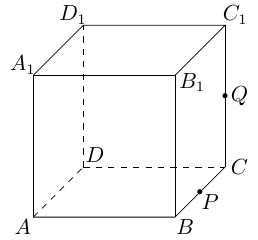
\includegraphics[width=4.8cm]{GaoKao/images/2013/anhui_liberal/q15_fig1.png}
\end{center}

\begin{enumerate}
\item 当 \(0 < CQ < \frac{1}{2}\) 时，\(S\) 为四边形；
\item 当 \(CQ = \frac{1}{2}\) 时，\(S\) 为等腰梯形；
\item 当 \(CQ = \frac{3}{4}\) 时，\(S\) 与 \(C_1D_1\) 交点 \(R\) 满足 \(C_1R = \frac{1}{3}\)；
\item 当 \(\frac{3}{4} < CQ < 1\) 时，\(S\) 为六边形；
\item 当 \(CQ = 1\) 时，\(S\) 的面积为 \(\frac{\sqrt{6}}{2}\).
\end{enumerate}

    \end{enumerate}

\end{description}

\begin{description}

    \item[三、解答题]

    \begin{enumerate}[leftmargin=5pt]

      \addtocounter{enumi}{+15}

        \item 设函数 \( f(x) = \sin x + \sin \left(x + \frac{\pi}{3}\right) \).
\begin{enumerate}
\item 求 \( f(x) \) 的最小值，并求使 \( f(x) \) 取得最小值的 \(x\) 的集合；
\item 不画图，说明函数 \( y = f(x) \) 的图象可由 \( y = \sin x \) 的图象经过怎样的变化得到.
\end{enumerate}

        \item 为调查甲，乙两校高三年级学生某次联考数学成绩情况. 用简单随机抽样，从这两校中各抽取 \(30\) 名高三年级学生，以他们的数学成绩（百分制）作为样本，样本数据的茎叶图如图：

\begin{enumerate}
\item 若甲校高三年级每位学生被抽取的概率为 \(0.05\)，求甲校高三年级学生总人数，并估计甲校高三年级这次联考数学成绩的及格率（\(60\) 分及 \(60\) 分以上为及格）；
\item 设甲，乙两校高三年级学生这次联考平均成绩分别为 \(\bar{x}_{1}\)，\(\bar{x}_{2}\)，估计 \( \bar{x}_{1} - \bar{x}_{2} \) 的值.
\end{enumerate}

\begin{center}
\begin{tabular}{r|c|l}
\multicolumn{1}{c}{甲} & \  & \multicolumn{1}{c}{乙} \\
\hline
\(7\) & 4 & \(5\) \\
\(5\;3\;3\;2\) & 5 & \(3\;3\;8\) \\
\(5\;5\;4\;3\;3\;3\;1\;0\;0\) & 6 & \(0\;0\;0\;1\;1\;2\;2\;3\;3\;5\) \\
\(8\;6\;6\;2\;2\;1\;1\;0\;0\) & 7 & \(0\;0\;2\;2\;2\;3\;3\;6\;6\;9\) \\
\(7\;5\;4\;4\;2\) & 8 & \(1\;1\;5\;5\;8\) \\
\(2\;0\) & 9 & \(0\)
\end{tabular}
\end{center}

        \item 如图，四棱锥 \(P - ABCD\) 的底面 \(ABCD\) 是边长为 \(2\) 的菱形，\(\angle BAD = 60^{\circ}\). 已知 \(PB = PD = 2\)，\(PA = \sqrt{6}\).

\begin{enumerate}
\item 证明： \(PC \perp BD\)；
\item 若 \(E\) 为 \(PA\) 的中点，求三棱锥 \(P - BCE\) 的体积.
\end{enumerate}

\begin{center}
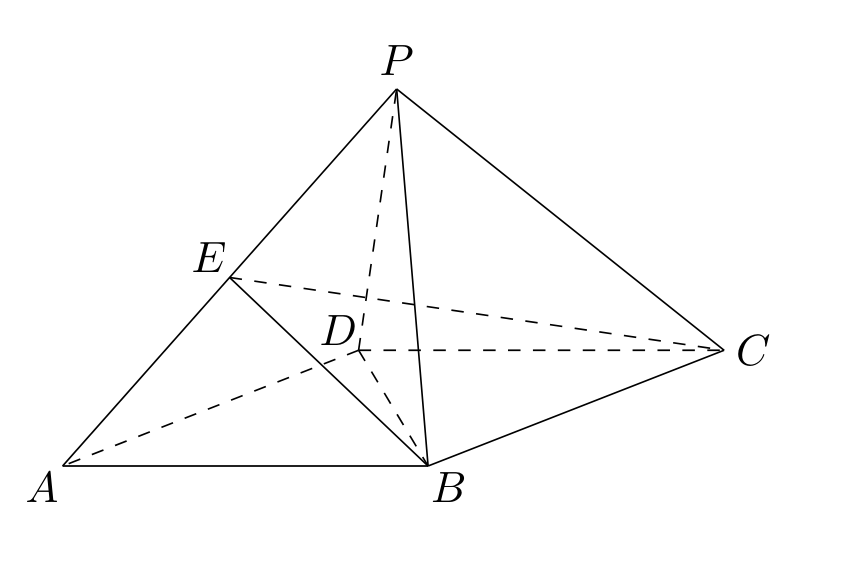
\includegraphics[width=0.34\linewidth]{GaoKao/images/2013/anhui_liberal/q18_fig1.png}
\end{center}

        \item 设数列 \(\{a_{n}\}\) 满足 \(a_{1} = 2\)，\(a_{2} + a_{4} = 8\)，且对任意 \(n \in \mathbb{N}^{*}\)，函数
\(f(x) = (a_{n} - a_{n+1} + a_{n+2})x + a_{n+1}\cos x - a_{n+2}\sin x\)
满足 \(f'\!\left(\frac{\pi}{2}\right) = 0\).

\begin{enumerate}
\item 求数列 \(\{a_{n}\}\) 的通项公式；
\item 若 \(b_{n} = 2\left(a_{n} + \frac{1}{2a_{n}}\right)\)，求数列 \(\{b_{n}\}\) 的前 \(n\) 项和 \(S_{n}\).
\end{enumerate}

        \item 设函数 \( f(x) = ax - (1 + a^2)x^2 \)，其中 \( a > 0 \)，区间 \( I = \{x \mid f(x) > 0\} \).
\begin{enumerate}
\item 求 \(I\) 的长度（注：区间 \((\alpha, \beta)\) 的长度定义为 \(\beta - \alpha\)）；
\item 给定常数 \(k \in (0,1)\)，当 \(1 - k \leqslant a \leqslant 1 + k\) 时，求 \(I\) 长度的最小值.
\end{enumerate}

        \item 已知椭圆 \(C: \frac{x^2}{a^2} + \frac{y^2}{b^2} = 1 \) （\(a > b > 0\)）的焦距为 \(4\)，且过点 \(P(\sqrt{2}, \sqrt{3})\).
\begin{enumerate}
\item 求椭圆 \(C\) 的方程.
\item 设 \(Q(x_0, y_0) \) （\(x_0 y_0 \neq 0\)）为椭圆 \(C\) 上一点，过点 \(Q\) 作 \(x\) 轴的垂线，垂足为 \(E\). 取点 \(A(0, 2\sqrt{2})\)，连接 \(AE\). 过点 \(A\) 作 \(AE\) 的垂线交 \(x\) 轴于点 \(D\). 点 \(G\) 是点 \(D\) 关于 \(y\) 轴的对称点，作直线 \(QG\). 问这样作出的直线 \(QG\) 是否与椭圆 \(C\) 一定有唯一的公共点？ 并说明理由.
\end{enumerate}

    \end{enumerate}

\end{description}


\subsection{2013年北京卷（理）}\label{gk:2013年北京卷（理）}

\begin{description}

    \item[一、选择题]

    \begin{enumerate}[leftmargin=5pt]

        \item 已知集合 \(A = \{-1, 0, 1\}\)，\(B = \{x \mid -1 \leqslant x < 1\}\)，则 \(A \cap B =\)（\quad）

        {\centering\begin{tabular*}{\linewidth}{@{}@{\extracolsep{\fill}}llll@{}}
          \text{A. }\(\{0\}\)  &  \text{B. }\( \{-1,0\} \)  &  \text{C. }\(\{0,1\}\)  &  \text{D. }\( \{-1, 0, 1\} \)
        \end{tabular*}\par}

        \item 在复平面内，复数 \((2 - \i)^2\) 对应的点位于（\quad）

        {\centering\begin{tabular*}{\linewidth}{@{}@{\extracolsep{\fill}}llll@{}}
          \text{A. }第一象限  &  \text{B. }第二象限  &  \text{C. }第三象限  &  \text{D. }第四象限
        \end{tabular*}\par}

        \item “\(\varphi = \pi\)”是“曲线 \(y = \sin (2x + \varphi)\) 过坐标原点”的（\quad）

        {\centering\begin{tabular*}{\linewidth}{@{}@{\extracolsep{\fill}}llll@{}}
          \text{A. }充分而不必要条件  &  \text{B. }必要而不充分条件  &  \text{C. }充分必要条件  &  \text{D. }既不充分也不必要条件
        \end{tabular*}\par}

        \item 执行如图所示的程序框图，输出的 \(S\) 值为（\quad）

\begin{center}
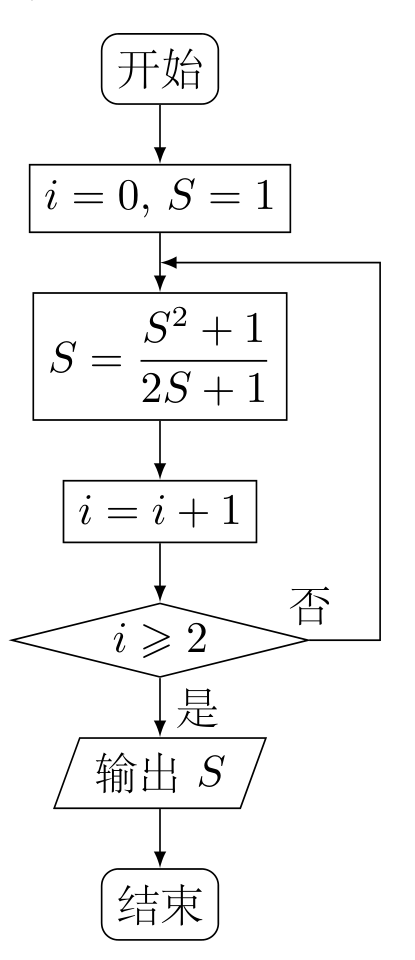
\includegraphics[width=0.32\linewidth]{GaoKao/images/2013/beijing_science/q4_fig1.png}
\end{center}

        {\centering\begin{tabular*}{\linewidth}{@{}@{\extracolsep{\fill}}llll@{}}
          \text{A. }1  &  \text{B. }\(\frac{2}{3}\)  &  \text{C. }\(\frac{13}{21}\)  &  \text{D. }\(\frac{610}{987}\)
        \end{tabular*}\par}

        \item 函数 \( f(x) \) 的图象向右平移 1 个单位长度，所得图象与曲线 \( y = {\mathrm{e}}^{x} \) 关于 \( y \) 轴对称，则 \( f(x) = \)（\quad）

        {\centering\begin{tabular*}{\linewidth}{@{}@{\extracolsep{\fill}}llll@{}}
          \text{A. }\({\mathrm{e}}^{x + 1}\)  &  \text{B. }\({\mathrm{e}}^{x - 1}\)  &  \text{C. }\({\mathrm{e}}^{-x + 1}\)  &  \text{D. }\({\mathrm{e}}^{-x - 1}\)
        \end{tabular*}\par}

        \item 若双曲线 \(\frac{x^2}{a^2} - \frac{y^2}{b^2} = 1\) 的离心率为 \(\sqrt{3}\)，则其渐近线方程为（\quad）

        {\centering\begin{tabular*}{\linewidth}{@{}@{\extracolsep{\fill}}llll@{}}
          \text{A. }\(y = \pm 2x\)  &  \text{B. }\(y = \pm \sqrt{2} x\)  &  \text{C. }\(y = \pm \frac{1}{2} x\)  &  \text{D. }\(y = \pm \frac{\sqrt{2}}{2} x\)
        \end{tabular*}\par}

        \item 直线 \(l\) 过抛物线 \(C: x^{2} = 4y\) 的焦点且与 \(y\) 轴垂直，则 \(l\) 与 \(C\) 所围成的图形的面积等于（\quad）

        {\centering\begin{tabular*}{\linewidth}{@{}@{\extracolsep{\fill}}llll@{}}
          \text{A. }\(\frac{4}{3}\)  &  \text{B. }2  &  \text{C. }\( \frac{8}{3} \)  &  \text{D. }\(\frac{16\sqrt{2}}{3}\)
        \end{tabular*}\par}

        \item 设关于 \(x\)，\(y\) 的不等式组 \(\begin{cases}
2x - y + 1 > 0,\\
x + m < 0,\\
y - m > 0
\end{cases}\) 表示的平面区域内存在点 \(P(x_0, y_0)\)，满足 \(x_0 - 2y_0 = 2\)，则 \(m\) 的取值范围是（\quad）

        {\centering\begin{tabular*}{\linewidth}{@{}@{\extracolsep{\fill}}llll@{}}
          \text{A. }\(\left(-\infty, \frac{4}{3}\right)\)  &  \text{B. }\(\left(-\infty, \frac{1}{3}\right)\)  &  \text{C. }\(\left(-\infty, -\frac{2}{3}\right)\)  &  \text{D. }\(\left(-\infty, -\frac{5}{3}\right)\)
        \end{tabular*}\par}

    \end{enumerate}

\end{description}

\begin{description}

    \item[二、填空题]

    \begin{enumerate}[leftmargin=5pt]

      \addtocounter{enumi}{+8}

        \item 在极坐标系中，点 \(\left(2, \frac{\pi}{6}\right)\) 到直线 \(\rho \sin \theta = 2\) 的距离等于\rule[-0.3ex]{3em}{0.4pt}.

        \item 若等比数列 \( \{a_{n}\} \) 满足 \(a_{2} + a_{4} = 20\)，\(a_{3} + a_{5} = 40\)，则公比 \(q =\)\rule[-0.3ex]{3em}{0.4pt}，前 \(n\) 项和 \( S_{n} = \)\rule[-0.3ex]{3em}{0.4pt}.

        \item 如图，\(A\) 为圆 \(O\) 的直径，\(PA\) 为圆 \(O\) 的切线，\(PB\) 与圆 \(O\) 相交于 \(D\)，若 \(PA = 3\)，\(PD:DB = 9:16\)，则 \(PD =\)\rule[-0.3ex]{3em}{0.4pt}，\(AB =\)\rule[-0.3ex]{3em}{0.4pt}.
\begin{center}
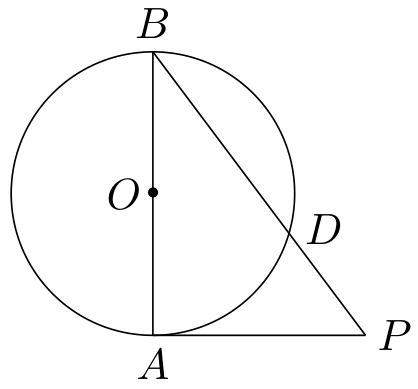
\includegraphics[width=5.0cm]{GaoKao/images/2013/beijing_science/q11_fig1.png}
\end{center}

        \item 将序号分别为 1， 2， 3， 4， 5 的 5 张参观券全部分给 4 人，每人至少 1 张，如果分给同一人的 2 张参观券连号，那么不同的分法种数是\rule[-0.3ex]{3em}{0.4pt}.

        \item 向量 \(\bm{a}, \bm{b}, \bm{c}\) 在正方形网格中的位置如图所示，若 \(\bm{c} = \lambda \bm{a} + \mu \bm{b}\)（\(\lambda, \mu \in \mathbb{R}\)），则 \(\frac{\lambda}{\mu} =\)\rule[-0.3ex]{3em}{0.4pt}.
\begin{center}
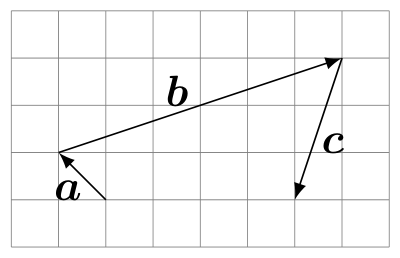
\includegraphics[width=3.3cm]{GaoKao/images/2013/beijing_science/q13_fig1.png}
\end{center}

        \item 如图，在棱长为 2 的正方体 \(ABCD - A_{1}B_{1}C_{1}D_{1}\) 中，\(E\) 为 \(BC\) 的中点，点 \(P\) 在线段 \(D_{1}E\) 上，点 \(P\) 到直线 \(CC_{1}\) 的距离的最小值为\rule[-0.3ex]{3em}{0.4pt}.
\begin{center}
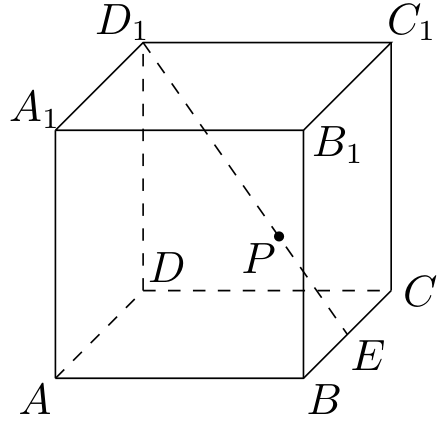
\includegraphics[width=4.6cm]{GaoKao/images/2013/beijing_science/q14_fig1.png}
\end{center}

    \end{enumerate}

\end{description}

\begin{description}

    \item[三、解答题]

    \begin{enumerate}[leftmargin=5pt]

      \addtocounter{enumi}{+14}

        \item 在 \(\triangle ABC\) 中，\(a = 3\)，\(b = 2\sqrt{6}\)，\(\angle B = 2\angle A\).
\begin{enumerate}
\item 求 \( \cos A \) 的值.
\item 求 \(c\) 的值.
\end{enumerate}

        \item 下图是某市 3 月 1 日至 14 日的空气质量指数趋势图，空气质量指数小于 100 表示空气质量优良，空气质量指数大于 200 表示空气重度污染. 某人随机选择 3 月 1 日至 3 月 13 日中的某一天到达该市，并停留 2 天.

\begin{enumerate}
\item 求此人到达当日空气重度污染的概率；
\item 设 \(X\) 是此人停留期间空气质量优良的天数，求 \(X\) 的分布列与数学期望；
\item 由图判断从哪天开始连续三天的空气质量指数方差最大（结论不要求证明）
\end{enumerate}

\begin{center}
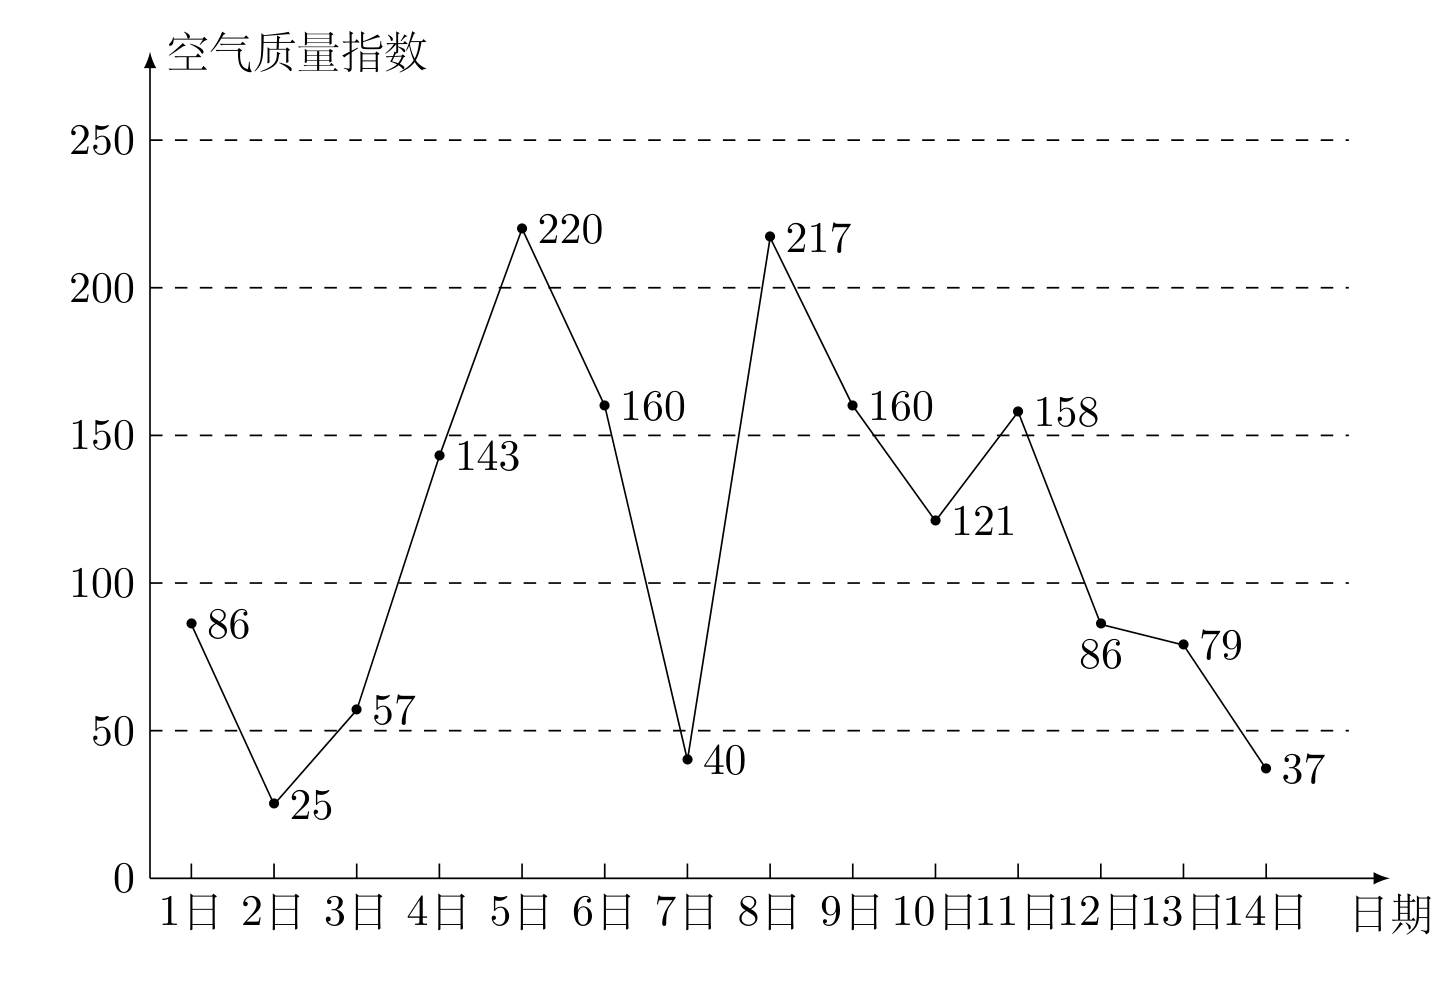
\includegraphics[width=16.0cm]{GaoKao/images/2013/beijing_science/q16_fig1.png}
\end{center}

        \item 如图，在三棱柱 \(ABC - A_{1}B_{1}C_{1}\) 中，\(AA_{1}C_{1}C\) 是边长为 4 的正方形. 平面 \(ABC \perp\) 平面 \(AA_{1}C_{1}C\)，\(AB = 3\)，\(BC = 5\).
\begin{enumerate}
\item 求证： \(AA_{1} \perp\) 平面 \(ABC\)；
\item 求二面角 \(A_{1} - BC_{1} - B_{1}\) 的余弦值；
\item 证明：在线段 \(BC_{1}\) 上存在点 \(D\)，使得 \(AD \perp A_{1}B\)，并求 \(\frac{BD}{BC_{1}}\) 的值.
\end{enumerate}
\begin{center}
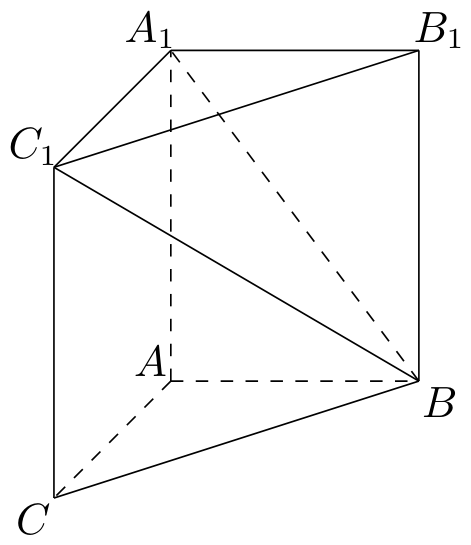
\includegraphics[width=4.7cm]{GaoKao/images/2013/beijing_science/q17_fig1.png}
\end{center}

        \item 设 \(L\) 为曲线 \(C: y = \frac{\ln x}{x}\) 在点 \((1,0)\) 处的切线.
\begin{enumerate}
\item 求 \(L\) 的方程；
\item 证明：除切点 \((1,0)\) 之外，曲线 \(C\) 在直线 \(L\) 的下方.
\end{enumerate}

        \item 已知 \(A\)，\(B\)，\(C\) 是椭圆 \(W: \frac{x^2}{4} + y^2 = 1\) 上的三个点，\(O\) 是坐标原点.
\begin{enumerate}
\item 当点 \(B\) 是 \(W\) 的右顶点，且四边形 \(OABC\) 为菱形时，求此菱形的面积；
\item 当点 \(B\) 不是 \(W\) 的顶点时，判断四边形 \(OABC\) 是否可能为菱形，并说明理由.
\end{enumerate}

        \item 已知 \(\{a_{n}\}\) 是由非负整数组成的无穷数列，该数列前 \(n\) 项的最大值记为 \(A_{n}\)，第 \(n\) 项之后各项 \(a_{n+1}\)，\(a_{n+2}\)，\(\cdots\) 的最小值记为 \(B_{n}\)，\(d_{n} = A_{n} - B_{n}\).
\begin{enumerate}
\item 若 \( \{a_{n}\} \) 为 2, 1, 4, 3, 2, 1, 4, 3, \( \cdots \)，是一个周期为 4 的数列 （即对任意 \(n \in \mathbb{N}^{*}\)，\(a_{n+4} = a_{n}\) ），写出 \(d_{1}\)，\(d_{2}\)，\(d_{3}\)，\(d_{4}\) 的值；
\item 设 \(d\) 是非负整数，证明： \(d_{n} = -d \) （\(n = 1, 2, 3 \cdots\)）的充分必要条件为 \(\{a_{n}\}\) 是公差为 \(d\) 的等差数列；
\item 证明：若 \(a_{1} = 2\)，\(d_{n} = 1 \)（\(n = 1, 2, 3, \cdots\)），则 \(\{a_{n}\}\) 的项只能是 1 或者 2，且有无穷多项为 1.
\end{enumerate}

    \end{enumerate}

\end{description}


\subsection{2013年北京卷（文）}\label{gk:2013年北京卷（文）}

\begin{description}

    \item[一、选择题]

    \begin{enumerate}[leftmargin=5pt]

        \item 已知集合 \(A = \{-1, 0, 1\}\)，\(B = \{x \mid -1 \leqslant x < 1\}\)，则 \(A \cap B =\)（\quad）

        {\centering\begin{tabular*}{\linewidth}{@{}@{\extracolsep{\fill}}llll@{}}
          \text{A. }\(\{0\}\)  &  \text{B. }\( \{-1,0\} \)  &  \text{C. }\(\{0,1\}\)  &  \text{D. }\(\{-1,0,1\}\)
        \end{tabular*}\par}

        \item 设 \(a\)，\(b\)，\(c \in \mathbb{R}\)，且 \(a > b\)，则（\quad）

        {\centering\begin{tabular*}{\linewidth}{@{}@{\extracolsep{\fill}}llll@{}}
          \text{A. }\(ac > bc\)  &  \text{B. }\(\frac{1}{a} \leqslant \frac{1}{b}\)  &  \text{C. }\(a^2 > b^2\)  &  \text{D. }\(a^3 > b^3\)
        \end{tabular*}\par}

        \item 下列函数中，既是偶函数又在区间 \((0, +\infty)\) 上单调递减的是（\quad）

        {\centering\begin{tabular*}{\linewidth}{@{}@{\extracolsep{\fill}}llll@{}}
          \text{A. }\(y = \frac{1}{x}\)  &  \text{B. }\( y = {\mathrm{e}}^{-x} \)  &  \text{C. }\( y = -x^{2} + 1 \)  &  \text{D. }\(y = \lg |x|\)
        \end{tabular*}\par}

        \item 在复平面内，复数 \( \i(2 - \i) \) 对应的点位于（\quad）

        {\centering\begin{tabular*}{\linewidth}{@{}@{\extracolsep{\fill}}llll@{}}
          \text{A. }第一象限  &  \text{B. }第二象限  &  \text{C. }第三象限  &  \text{D. }第四象限
        \end{tabular*}\par}

        \item 在 \(\triangle ABC\) 中，\(a = 3\)，\(b = 5\)，\(\sin A = \frac{1}{3}\)，则 \(\sin B =\)（\quad）

        {\centering\begin{tabular*}{\linewidth}{@{}@{\extracolsep{\fill}}llll@{}}
          \text{A. }\( \frac{1}{5} \)  &  \text{B. }\( \frac{5}{9} \)  &  \text{C. }\( \frac{\sqrt{5}}{3} \)  &  \text{D. }\(1\)
        \end{tabular*}\par}

        \item 执行如图所示的程序框图，输出的 \(S\) 值为（\quad）

\begin{center}
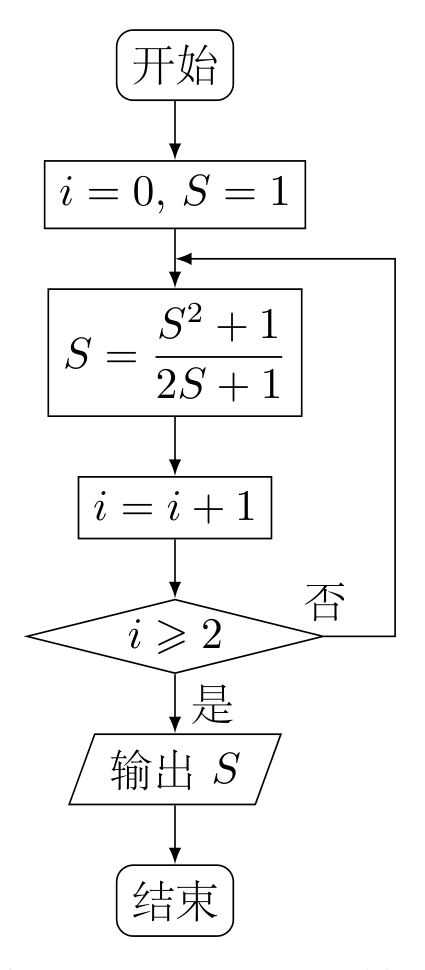
\includegraphics[width=0.30\linewidth]{GaoKao/images/2013/beijing_liberal/q6_fig1.png}
\end{center}

        {\centering\begin{tabular*}{\linewidth}{@{}@{\extracolsep{\fill}}llll@{}}
          \text{A. }\(1\)  &  \text{B. }\( \frac{2}{3} \)  &  \text{C. }\( \frac{13}{21} \)  &  \text{D. }\( \frac{610}{987} \)
        \end{tabular*}\par}

        \item 双曲线 \(x^{2} - \frac{y^{2}}{m} = 1\) 的离心率大于 \(\sqrt{2}\) 的充分必要条件是（\quad）

        {\centering\begin{tabular*}{\linewidth}{@{}@{\extracolsep{\fill}}llll@{}}
          \text{A. }\(m > \frac{1}{2}\)  &  \text{B. }\(m \geqslant 1\)  &  \text{C. }\(m > 1\)  &  \text{D. }\(m > 2\)
        \end{tabular*}\par}

        \item 如图，在正方体 \(ABCD - A_{1}B_{1}C_{1}D_{1}\) 中，\(P\) 为对角线 \(BD_{1}\) 的三等分点，\(P\) 到各顶点的距离的不同取值有（\quad）

\begin{center}
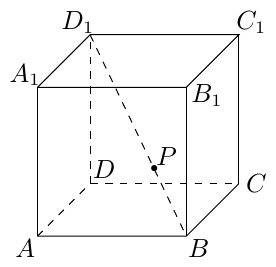
\includegraphics[width=4.7cm]{GaoKao/images/2013/beijing_liberal/q8_fig1.png}
\end{center}

        {\centering\begin{tabular*}{\linewidth}{@{}@{\extracolsep{\fill}}llll@{}}
          \text{A. }\(3\) 个  &  \text{B. }\(4\) 个  &  \text{C. }\(5\) 个  &  \text{D. }\(6\) 个
        \end{tabular*}\par}

    \end{enumerate}

\end{description}

\begin{description}

    \item[二、填空题]

    \begin{enumerate}[leftmargin=5pt]

      \addtocounter{enumi}{+8}

        \item 若抛物线 \( y^{2}=2px \) 的焦点坐标为 \( (1,0) \)，则 \(p=\)\rule[-0.3ex]{3em}{0.4pt}；准线方程为\rule[-0.3ex]{3em}{0.4pt}.

        \item 某四棱锥的三视图如图所示，该四棱锥的体积为\rule[-0.3ex]{3em}{0.4pt}.

\begin{center}
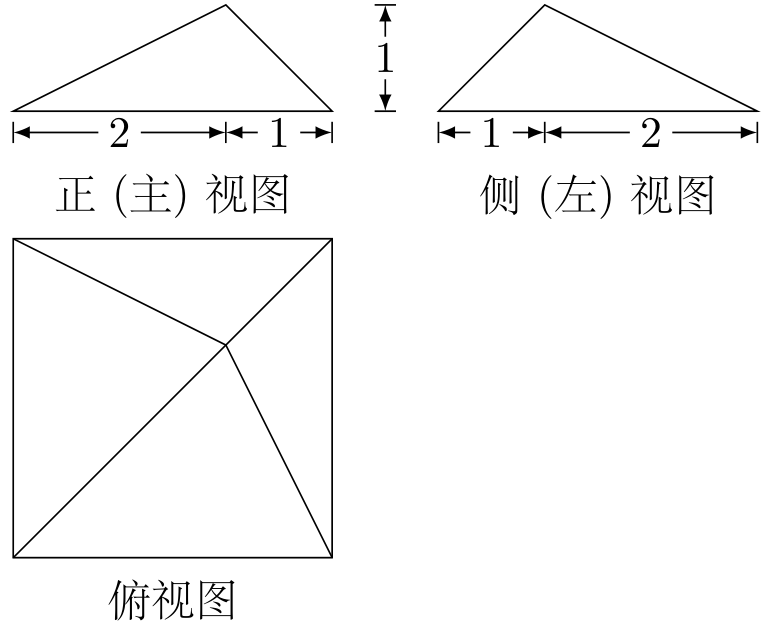
\includegraphics[width=7.6cm]{GaoKao/images/2013/beijing_liberal/q10_fig1.png}
\end{center}

        \item 若等比数列 \(\{a_{n}\}\) 满足 \(a_{2} + a_{4} = 20\)，\(a_{3} + a_{5} = 40\)，则公比 \(q = \)\rule[-0.3ex]{3em}{0.4pt} . 前 \(n\) 项和 \(S_{n} =\)\rule[-0.3ex]{3em}{0.4pt}.

        \item 设 \(D\) 为不等式组 \(\begin{cases}
x \geqslant 0,\\
2x - y \leqslant 0,\\
x + y - 3 \leqslant 0
\end{cases}\) 表示的平面区域. 区域 \(D\) 上的点与点 \((1,0)\) 之间的距离的最小值为\rule[-0.3ex]{3em}{0.4pt}.

        \item 函数 \( f(x)=\begin{cases}
\log_{\frac{1}{2}}x,&x\geqslant1,\\
2^{x},&x<1
\end{cases} \) 的值域为\rule[-0.3ex]{3em}{0.4pt}.

        \item 已知点 \(A(1, -1)\)，\(B(3, 0)\)，\(C(2, 1)\). 若平面区域 \(D\) 由所有满足 \(\overrightarrow{AP} = \lambda \overrightarrow{AB} + \mu \overrightarrow{AC}\) （\(1 \leqslant \lambda \leqslant 2\)，\(0 \leqslant \mu \leqslant 1\)） 的点 \(P\) 组成. 则 \(D\) 的面积为\rule[-0.3ex]{3em}{0.4pt}.

    \end{enumerate}

\end{description}

\begin{description}

    \item[三、解答题]

    \begin{enumerate}[leftmargin=5pt]

      \addtocounter{enumi}{+14}

        \item 已知函数 \( f(x) = (2\cos^2 x - 1)\sin 2x + \frac{1}{2}\cos 4x \).
\begin{enumerate}
\item 求 \( f(x) \) 的最小正周期及最大值；
\item 若 \(\alpha \in \left(\frac{\pi}{2}, \pi\right)\)，且 \(f(\alpha) = \frac{\sqrt{2}}{2}\)，求 \(\alpha\) 的值.
\end{enumerate}

        \item 下图是某市3月1日至14日的空气质量指数趋势图，空气质量指数小于100表示空气质量优良，空气质量指数大于200表示空气重度污染. 某人随机选择3月1日至3月13日中的某一天到达该市，并停留2天.

\begin{enumerate}
\item 求此人到达当日空气质量优良的概率；
\item 求此人在该市停留期间只有 1 天空气质量重度污染的概率；
\item 由图判断从哪天开始连续三天的空气质量指数方差最大？（结论不要求证明）
\end{enumerate}

\begin{center}
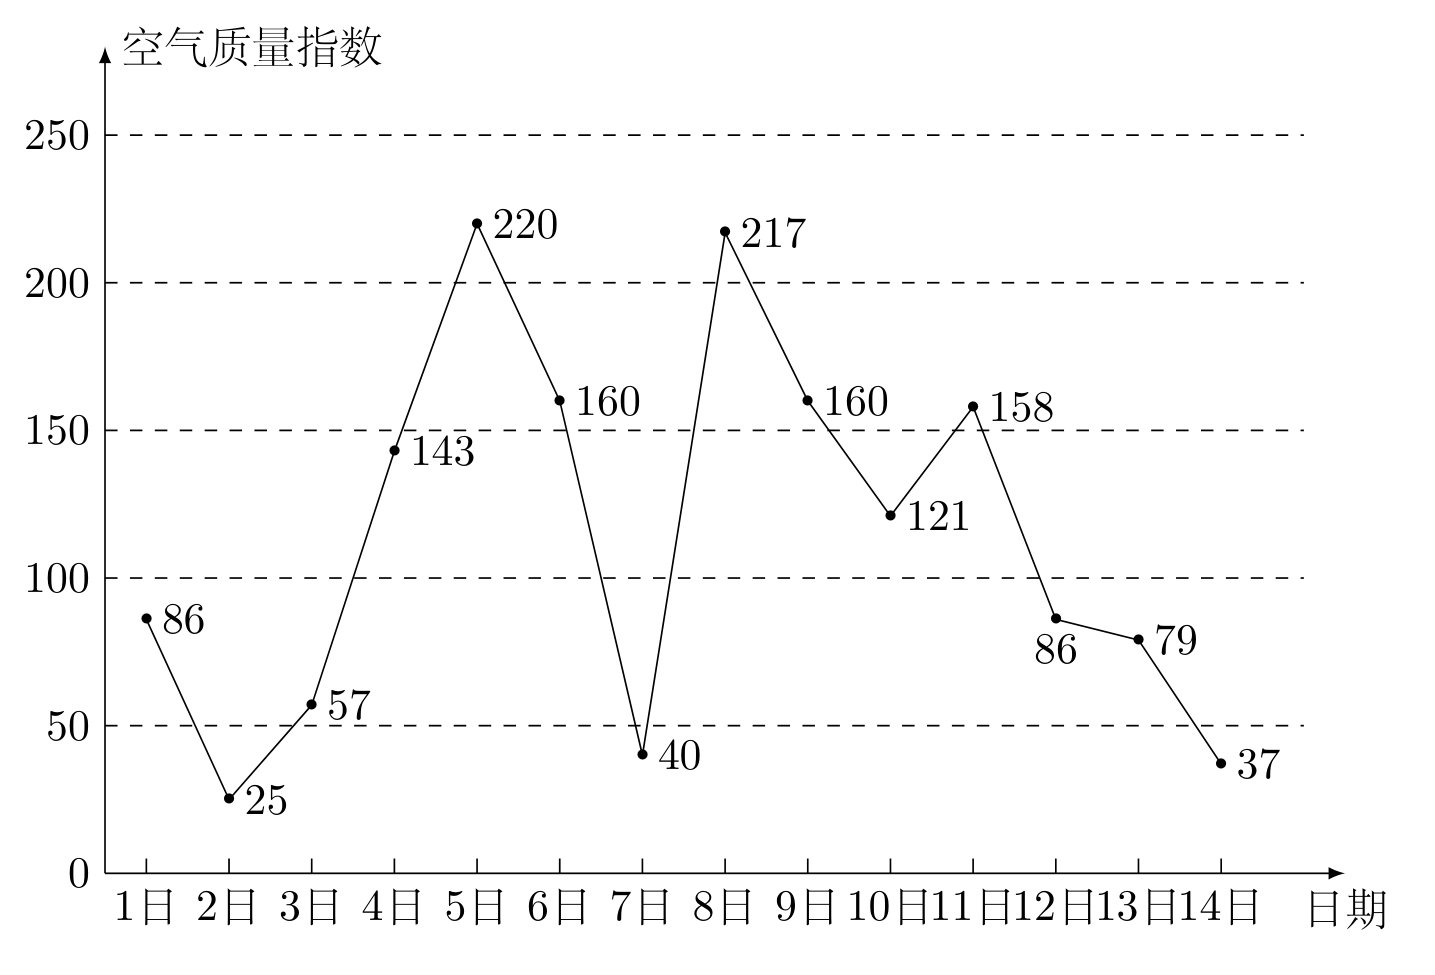
\includegraphics[width=16.0cm]{GaoKao/images/2013/beijing_liberal/q16_fig1.png}
\end{center}

        \item 如图，在四棱锥 \(P - ABCD\) 中，\(AB \parallel CD\)，\(AB \perp AD\)，\(CD = 2AB\)，平面 \(PAD \perp\) 底面 \(ABCD\)，\(PA \perp AD\)，\(E\) 和 \(F\) 分别是 \(CD\) 和 \(PC\) 的中点.

求证：
\begin{enumerate}
\item \(PA \perp\) 底面 \(ABCD\)；
\item \(BE \parallel\) 平面 \(PAD\)；
\item 平面 \(BEF \perp\) 平面 \(PCD\).
\end{enumerate}

\begin{center}
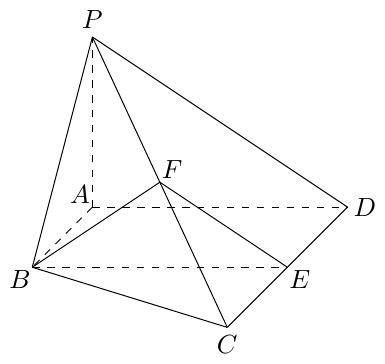
\includegraphics[width=8.0cm]{GaoKao/images/2013/beijing_liberal/q17_fig1.png}
\end{center}

        \item 直线 \( y = kx + m  \) （\(m \neq 0\)）与椭圆 \( W: \frac{x^2}{4} + y^2 = 1 \) 相交于 \(A\)，\(C\) 两点，\(O\) 是坐标原点.
\begin{enumerate}
\item 当点 \(B\) 的坐标为 \((0,1)\)，且四边形 \(OABC\) 为菱形时，求 \(AC\) 的长；
\item 当点 \(B\) 在 \(W\) 上且不是 \(W\) 的顶点时，证明：四边形 \(OABC\) 不可能为菱形.
\end{enumerate}

        \item 给定数列 \(a_1\)，\(a_2\)，\(\cdots\)，\(a_n\)，对 \(i = 1\)，\(2\)，\(\cdots\)，\(n-1\)，该数列前 \(i\) 项的最大值记为 \(A_i\)，后 \(n-i\) 项 \(a_{i+1}\)，\(a_{i+2}\)，\(\cdots\)，\(a_n\) 的最小值记为 \(B_i\)，\(d_i = A_i - B_i\).
\begin{enumerate}
\item 设数列 \(\{a_n\}\) 为 3， 4， 7， 1，写出 \(d_1\)，\(d_2\)，\(d_3\) 的值；
\item 设 \(a_1\)，\(a_2\)，\(\cdots\)，\(a_n\ \) （\(n \geqslant 4\)）是公比大于 1 的等比数列，且 \(a_1 > 0\). 证明： \(d_1\)，\(d_2\)，\(\cdots\)，\(d_{n-1}\) 是等比数列；
\item 设 \(d_1\)，\(d_2\)，\(\cdots\)，\(d_{n-1}\) 是公差大于 0 的等差数列，且 \(d_1 > 0\). 证明： \(a_1\)，\(a_2\)，\(\cdots\)，\(a_{n-1}\) 是等差数列.
\end{enumerate}

        \item 已知函数 \( f(x) = x^2 + x \sin x + \cos x \).
\begin{enumerate}
\item 若曲线 \( y = f(x) \) 在点 \((a, f(a))\) 处与直线 \( y = b \) 相切，求 \( a \) 与 \( b \) 的值；
\item 若曲线 \( y = f(x) \) 与直线 \( y = b \) 有两个不同交点，求 \( b \) 的取值范围.
\end{enumerate}

    \end{enumerate}

\end{description}


\subsection{2013年重庆卷（理）}\label{gk:2013年重庆卷（理）}

\begin{description}

    \item[一、选择题]

    \begin{enumerate}[leftmargin=5pt]

        \item 已知全集 \(U = \{1, 2, 3, 4\}\)，集合 \(A = \{1, 2\}\)，\(B = \{2, 3\}\)，则 \(\complement_U (A \cup B) =\)（\quad）

        {\centering\begin{tabular*}{\linewidth}{@{}@{\extracolsep{\fill}}llll@{}}
          \text{A. }\(\{1,3,4\}\)  &  \text{B. }\(\{3,4\}\)  &  \text{C. }\(\{3\}\)  &  \text{D. }\(\{4\}\)
        \end{tabular*}\par}

        \item 命题“对任意 \(x \in \mathbb{R}\)，都有 \(x^2 \geqslant 0\)”的否定为（\quad）

        {\centering\begin{tabular*}{\linewidth}{@{}@{\extracolsep{\fill}}llll@{}}
          \text{A. }对任意 \(x \in \mathbb{R}\)，都有 \(x^2 < 0\)  &  \text{B. }不存在 \(x \in \mathbb{R}\)，使得 \(x^2 < 0\)  &  \text{C. }存在 \(x_0 \in \mathbb{R}\)，使得 \(x_0^2 \geqslant 0\)  &  \text{D. }存在 \(x_0 \in \mathbb{R}\)，使得 \(x_0^2 < 0\)
        \end{tabular*}\par}

        \item \(\sqrt{(3 - a)(a + 6)} \) （\(-6\leqslant a\leqslant 3\)）的最大值为（\quad）

        {\centering\begin{tabular*}{\linewidth}{@{}@{\extracolsep{\fill}}llll@{}}
          \text{A. }\(9\)  &  \text{B. }\( \frac{9}{2} \)  &  \text{C. }\(3\)  &  \text{D. }\(\frac{3\sqrt{2}}{2}\)
        \end{tabular*}\par}

        \item 以下茎叶图记录了甲，乙两组各 \(5\) 名学生在一次英语听力测试中的成绩（单位：分）.

\begin{center}
\begin{tabular}{r|c|l}
\multicolumn{1}{c}{甲组} & & \multicolumn{1}{c}{乙组} \\
\hline
\(9\) & 0 & \(9\) \\
\(\mathit{x}\;2\) & 1 & \(5\;\mathit{y}\;8\) \\
\(7\;4\) & 2 & \(4\)
\end{tabular}
\end{center}

已知甲组数据的中位数为 \(15\)，乙组数据的平均数为 \(16.8\)，则 \(x\)，\(y\) 的值分别为（\quad）

        {\centering\begin{tabular*}{\linewidth}{@{}@{\extracolsep{\fill}}llll@{}}
          \text{A. }\(2\)，\(5\)  &  \text{B. }\(5\)，\(5\)  &  \text{C. }\(5\)，\(8\)  &  \text{D. }\(8\)，\(8\)
        \end{tabular*}\par}

        \item 某几何体的三视图如图所示，则该几何体的体积为（\quad）

\begin{center}
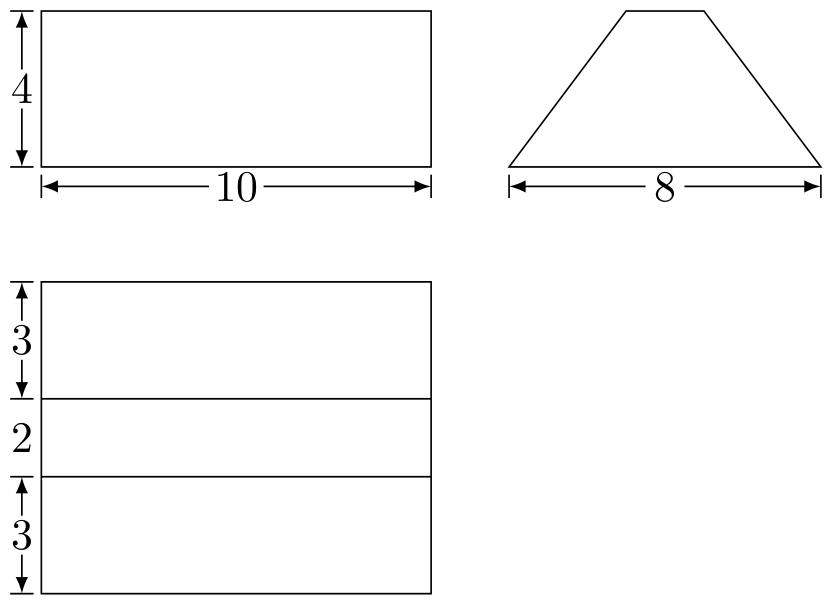
\includegraphics[width=8.0cm]{GaoKao/images/2013/chongqing_science/q5_fig1.png}
\end{center}

        {\centering\begin{tabular*}{\linewidth}{@{}@{\extracolsep{\fill}}llll@{}}
          \text{A. }\(\frac{560}{3}\)  &  \text{B. }\(\frac{580}{3}\)  &  \text{C. }\(200\)  &  \text{D. }\(240\)
        \end{tabular*}\par}

        \item 若 \(a < b < c\)，则函数 \(f(x) = (x - a)(x - b) + (x - b)(x - c) + (x - c)(x - a)\) 的两个零点分别位于区间（\quad）

        {\centering\begin{tabular*}{\linewidth}{@{}@{\extracolsep{\fill}}llll@{}}
          \text{A. }\((a, b)\) 和 \((b, c)\) 内  &  \text{B. }\((-\infty, a)\) 和 \((a, b)\) 内  &  \text{C. }\((b, c)\) 和 \((c, +\infty)\) 内  &  \text{D. }\((-\infty, a)\) 和 \((c, +\infty)\) 内
        \end{tabular*}\par}

        \item 已知圆 \(C_{1}: (x - 2)^{2} + (y - 3)^{2} = 1\)，圆 \(C_{2}: (x - 3)^{2} + (y - 4)^{2} = 9\)，\(M\)，\(N\) 分别是圆 \(C_{1}\)，\(C_{2}\) 上的动点，\(P\) 为 \(x\) 轴上的动点，则 \(|PM| + |PN|\) 的最小值为（\quad）

        {\centering\begin{tabular*}{\linewidth}{@{}@{\extracolsep{\fill}}llll@{}}
          \text{A. }\(5\sqrt{2} - 4\)  &  \text{B. }\(\sqrt{17} - 1\)  &  \text{C. }\(6 - 2\sqrt{2}\)  &  \text{D. }\(\sqrt{17}\)
        \end{tabular*}\par}

        \item 执行如图所示的程序框图，如果输出 \(s = 3\)，那么判断框内应填入的条件是（\quad）

\begin{center}
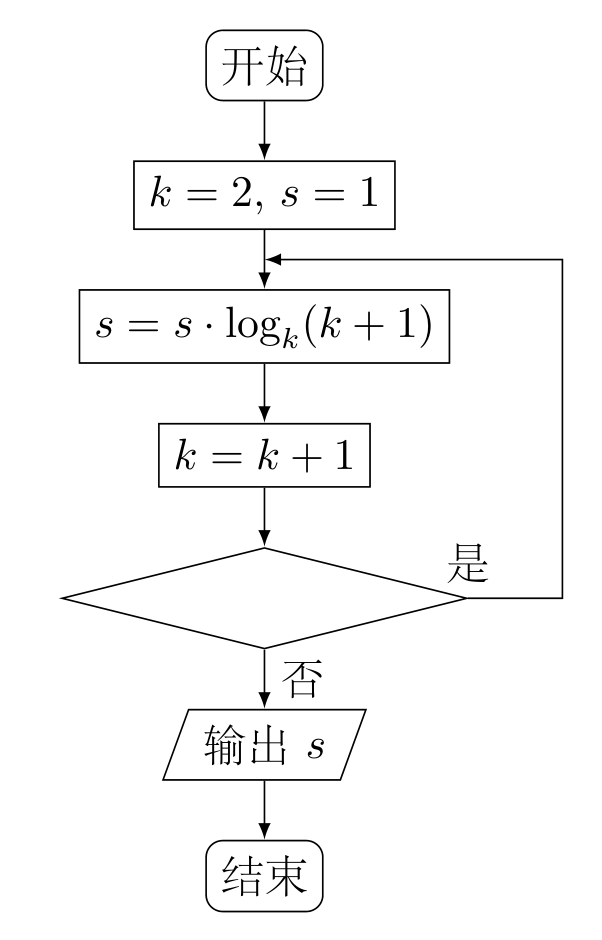
\includegraphics[width=0.38\linewidth]{GaoKao/images/2013/chongqing_science/q8_fig1.png}
\end{center}

        {\centering\begin{tabular*}{\linewidth}{@{}@{\extracolsep{\fill}}llll@{}}
          \text{A. }\(k \leqslant 6\)  &  \text{B. }\(k \leqslant 7\)  &  \text{C. }\(k \leqslant 8\)  &  \text{D. }\(k \leqslant 9\)
        \end{tabular*}\par}

        \item \(4\cos 50^{\circ} - \tan 40^{\circ} =\)（\quad）

        {\centering\begin{tabular*}{\linewidth}{@{}@{\extracolsep{\fill}}llll@{}}
          \text{A. }\(\sqrt{2}\)  &  \text{B. }\(\frac{\sqrt{2} + \sqrt{3}}{2}\)  &  \text{C. }\(\sqrt{3}\)  &  \text{D. }\(2\sqrt{2} - 1\)
        \end{tabular*}\par}

        \item 在平面上，\(\overrightarrow{AB_1} \perp \overrightarrow{AB_2}\)，\(|\overrightarrow{OB_1}| = |\overrightarrow{OB_2}| = 1\)，\(\overrightarrow{AP} = \overrightarrow{AB_1} + \overrightarrow{AB_2}\). 若 \(|\overrightarrow{OP}| < \frac{1}{2}\)，则 \(|\overrightarrow{OA}|\) 的取值范围是（\quad）

        {\centering\begin{tabular*}{\linewidth}{@{}@{\extracolsep{\fill}}llll@{}}
          \text{A. }\(\left(0, \frac{\sqrt{5}}{2}\right]\)  &  \text{B. }\(\left(\frac{\sqrt{5}}{2}, \frac{\sqrt{7}}{2}\right]\)  &  \text{C. }\(\left(\frac{\sqrt{5}}{2}, \sqrt{2}\right]\)  &  \text{D. }\(\left(\frac{\sqrt{7}}{2}, \sqrt{2}\right]\)
        \end{tabular*}\par}

    \end{enumerate}

\end{description}

\begin{description}

    \item[二、填空题]

    \begin{enumerate}[leftmargin=5pt]

      \addtocounter{enumi}{+10}

        \item 已知复数 \( z = \frac{5\i}{1 + 2\i} \)（\(\i\) 是虚数单位），则 \( |z| = \)\rule[-0.3ex]{3em}{0.4pt}.

        \item 已知 \( \{a_{n}\} \) 是等差数列，\( a_{1}=1 \)，公差 \( d\neq0 \)，\( S_{n} \) 为其前 \( n \) 项和. 若 \(a_{1}\)，\(a_{2}\)，\(a_{5}\) 成等比数列，则 \( S_{8}= \)\rule[-0.3ex]{3em}{0.4pt}.

        \item 从 \(3\) 名骨科、\(4\) 名脑外科和 \(5\) 名内科医生中选派 \(5\) 人组成一个抗震救灾医疗小组，骨科、脑外科和内科医生都至少有 \(1\) 人的选派方法种数是\rule[-0.3ex]{3em}{0.4pt}.

        \item 如图，在 \(\triangle ABC\) 中，\(\angle C = 90^{\circ}\)，\(\angle A = 60^{\circ}\)，\(AB = 20\)，过 \(C\) 作 \(\triangle ABC\) 的外接圆的切线 \(CD\)，\(BD \perp CD\)，\(BD\) 与外接圆交于点 \(E\)，则 \(DE\) 的长为\rule[-0.3ex]{3em}{0.4pt}.

\begin{center}
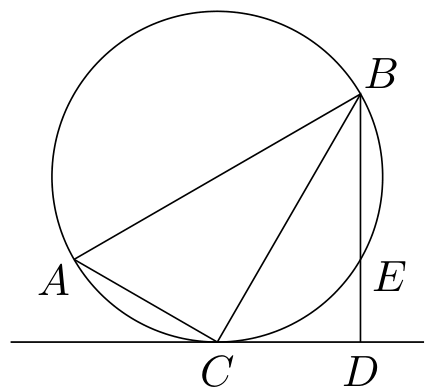
\includegraphics[width=5.8cm]{GaoKao/images/2013/chongqing_science/q14_fig1.png}
\end{center}

        \item 在直角坐标系 \(xOy\) 中，以原点 \(O\) 为极点，\(x\) 轴的正半轴为极轴建立极坐标系. 若极坐标方程为 \(\rho\cos \theta = 4\) 的直线与曲线 \(\begin{cases}
x = t^2,\\
y = t^3,
\end{cases}\) （\(t\) 为参数）相交于 \(A\)，\(B\) 两点，则 \(|AB| =\rule[-0.3ex]{3em}{0.4pt}\).

        \item 若关于实数 \(x\) 的不等式 \(|x - 5| + |x + 3| < a\) 无解，则实数 \(a\) 的取值范围是\rule[-0.3ex]{3em}{0.4pt}.

    \end{enumerate}

\end{description}

\begin{description}

    \item[三、解答题]

    \begin{enumerate}[leftmargin=5pt]

      \addtocounter{enumi}{+16}

        \item 设 \( f(x) = a(x - 5)^2 + 6\ln x \)，其中 \( a \in \mathbb{R} \)，曲线 \( y = f(x) \) 在点 \((1, f(1))\) 处的切线与 \( y \) 轴相交于点 \((0, 6)\).
\begin{enumerate}
\item 确定 \(a\) 的值；
\item 求函数 \( f(x) \) 的单调区间与极值.
\end{enumerate}

        \item 某商场举行的“三色球”购物摸奖活动规定：在一次摸奖中，摸奖者先从装有 \(3\) 个红球与 \(4\) 个白球的袋中任意摸出 \(3\) 个球，再从装有 \(1\) 个蓝球与 \(2\) 个白球的袋中任意摸出 \(1\) 个球，根据摸出 \(4\) 个球中红球与蓝球的个数，设一、二、三等奖如下：

\begin{center}
\renewcommand{\arraystretch}{1.2}
\begin{tabular}{|c|c|c|}
\hline
奖级 & 摸出红、蓝球个数 & 获奖金额 \\
\hline
一等奖 & \(3\) 红 \(1\) 蓝 & \(200\text{ 元}\) \\
\hline
二等奖 & \(3\) 红 \(0\) 蓝 & \(50\text{ 元}\) \\
\hline
三等奖 & \(2\) 红 \(1\) 蓝 & \(10\text{ 元}\) \\
\hline
\end{tabular}
\end{center}

其余情况无奖且每次摸奖最多只能获得一个奖级.
\begin{enumerate}
\item 求一次摸球恰好摸到 \(1\) 个红球的概率；
\item 求摸奖者在一次摸奖中获奖金额 \(X\) 的分布列与期望 \( E(X) \).
\end{enumerate}

        \item 如图，四棱锥 \(P - ABCD\) 中，\(PA \perp\) 底面 \(ABCD\)，\(BC = CD = 2\)，\(AC = 4\)，\(\angle ACB = \angle ACD = \frac{\pi}{3}\)，\(F\) 为 \(PC\) 的中点，\(AF \perp PB\).

\begin{enumerate}
\item 求 \(PA\) 的长；
\item 求二面角 \(B - AF - D\) 的正弦值.
\end{enumerate}

\begin{center}
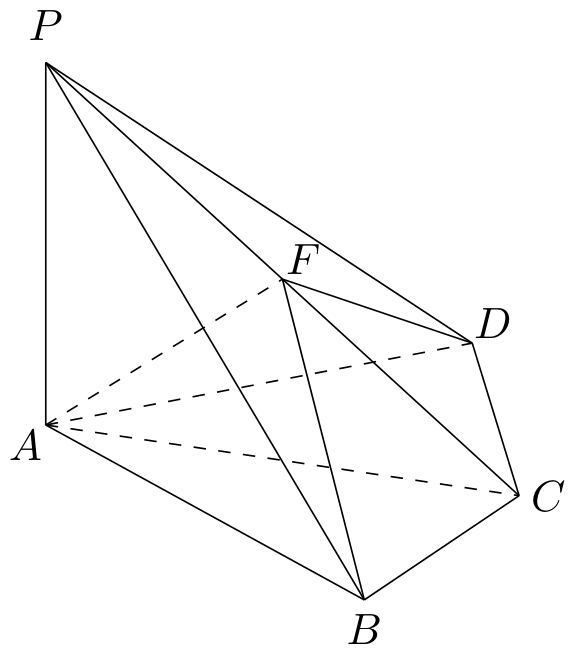
\includegraphics[width=7.1cm]{GaoKao/images/2013/chongqing_science/q19_fig1.png}
\end{center}

        \item 在 \(\triangle ABC\) 中，内角 \(A\)，\(B\)，\(C\) 的对边分别是 \(a\)，\(b\)，\(c\)，且 \(a^2 + b^2 + \sqrt{2}ab = c^2\).
\begin{enumerate}
\item 求 \(C\)；
\item 设 \(\cos A\cos B = \frac{3\sqrt{2}}{5}\)，\(\frac{\cos(\alpha + A)\cos(\alpha + B)}{\cos^2\alpha} = \frac{\sqrt{2}}{5}\)，求 \(\tan \alpha\) 的值.
\end{enumerate}

        \item 如图，椭圆的中心为原点 \(O\)，长轴在 \(x\) 轴上，离心率 \(e = \frac{\sqrt{2}}{2}\)，过左焦点 \(F_{1}\) 作 \(x\) 轴的垂线交椭圆于 \(A\)，\(A'\) 两点，\(|AA'| = 4\).

\begin{enumerate}
\item 求该椭圆的标准方程；
\item 取垂直于 \(x\) 轴的直线与椭圆相交于不同的两点 \(P\)，\(P'\)，过 \(P\)，\(P'\) 作圆心为 \(Q\) 的圆. 使椭圆上的其余点均在圆 \(Q\) 外. 若 \(PQ \perp P'Q\)，求圆 \(Q\) 的标准方程.
\end{enumerate}

\begin{center}
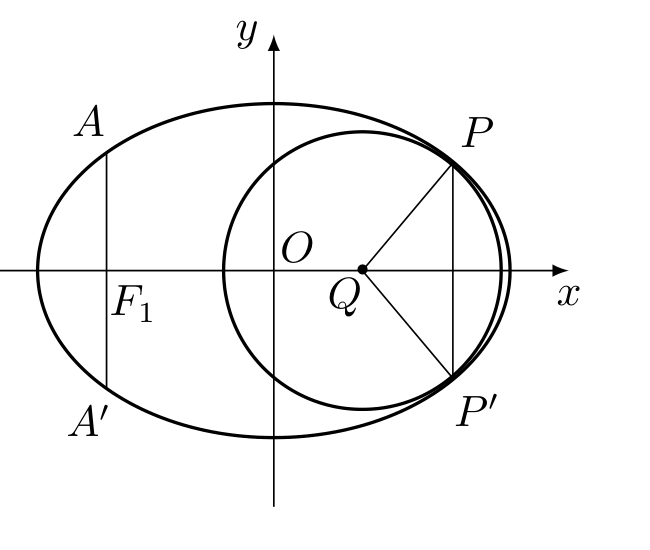
\includegraphics[width=6.2cm]{GaoKao/images/2013/chongqing_science/q21_fig1.png}
\end{center}

        \item 对正整数 \(n\)，记 \(I_n = \{1, 2, \cdots, n\}\)，\(P_n = \left\{\frac{m}{\sqrt{k}} \mid m \in I_n, k \in I_n\right\}\).
\begin{enumerate}
\item 求集合 \(P_{7}\) 中元素的个数；
\item 若 \(P_{n}\) 的子集 \(A\) 中任意两个元素之和不是整数的平方，则称 \(A\) 为“稀疏集”，求 \(n\) 的最大值，使 \(P_{n}\) 能分成两个不相交的稀疏集的并.
\end{enumerate}

    \end{enumerate}

\end{description}


\subsection{2013年重庆卷（文）}\label{gk:2013年重庆卷（文）}

\begin{description}

    \item[一、选择题]

    \begin{enumerate}[leftmargin=5pt]

        \item 已知全集 \(U = \{1, 2, 3, 4\}\)，集合 \(A = \{1, 2\}\)，\(B = \{2, 3\}\)，则 \(\complement_U (A \cup B) =\)（\quad）

        {\centering\begin{tabular*}{\linewidth}{@{}@{\extracolsep{\fill}}llll@{}}
          \text{A. }\(\{1,3,4\}\)  &  \text{B. }\(\{3,4\}\)  &  \text{C. }\(\{3\}\)  &  \text{D. }\(\{4\}\)
        \end{tabular*}\par}

        \item 命题“对任意 \(x \in \mathbb{R}\)，都有 \(x^2 \geqslant 0\)”的否定为（\quad）

        {\centering\begin{tabular*}{\linewidth}{@{}@{\extracolsep{\fill}}llll@{}}
          \text{A. }存在 \(x_0 \in \mathbb{R}\)，使得 \(x_0^2 < 0\)  &  \text{B. }不存在 \(x \in \mathbb{R}\)，使得 \(x^2 < 0\)  &  \text{C. }存在 \(x_0 \in \mathbb{R}\)，使得 \(x_0^2 \geqslant 0\)  &  \text{D. }对任意 \(x \in \mathbb{R}\)，都有 \(x^2 < 0\)
        \end{tabular*}\par}

        \item 函数 \( y = \frac{1}{\log_2(x - 2)} \) 的定义域是（\quad）

        {\centering\begin{tabular*}{\linewidth}{@{}@{\extracolsep{\fill}}llll@{}}
          \text{A. }\((-\infty, 2)\)  &  \text{B. }\((2, +\infty)\)  &  \text{C. }\((2,3)\cup (3, + \infty)\)  &  \text{D. }\((2,4)\cup (4, + \infty)\)
        \end{tabular*}\par}

        \item 设 \(P\) 是圆 \((x - 3)^2 + (y + 1)^2 = 4\) 上的动点，\(Q\) 是直线 \(x = -3\) 上的动点，则 \(|PQ|\) 的最小值为（\quad）

        {\centering\begin{tabular*}{\linewidth}{@{}@{\extracolsep{\fill}}llll@{}}
          \text{A. }\(6\)  &  \text{B. }\(4\)  &  \text{C. }\(3\)  &  \text{D. }\(2\)
        \end{tabular*}\par}

        \item 执行如图所示的程序框图，则输出的 \(k\) 的值是（\quad）

\begin{center}
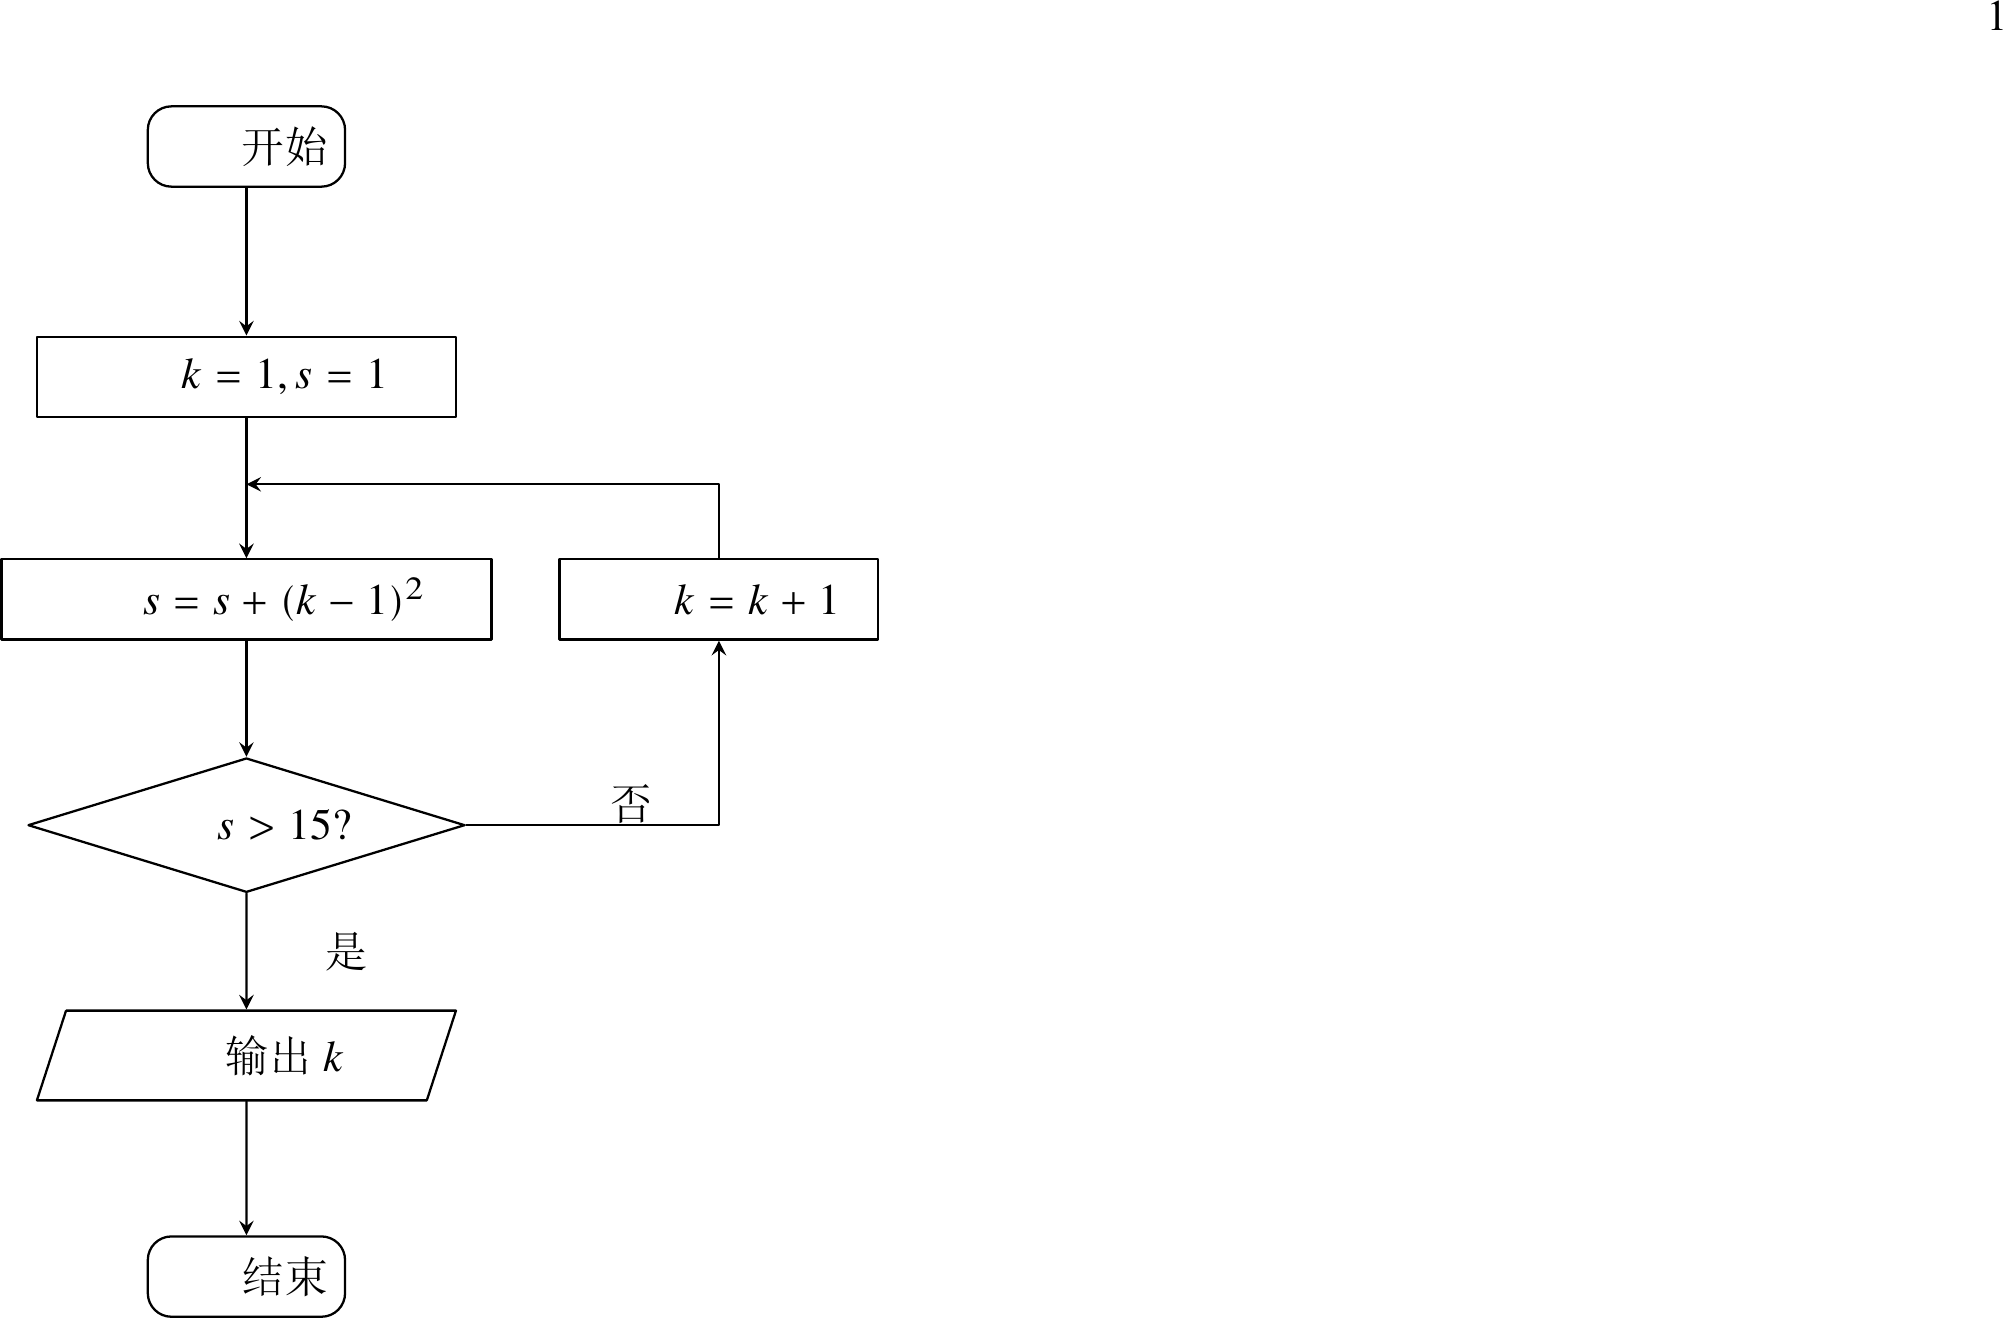
\includegraphics[width=0.42\linewidth]{GaoKao/images/2013/chongqing_liberal/q5_fig1.png}
\end{center}

        {\centering\begin{tabular*}{\linewidth}{@{}@{\extracolsep{\fill}}llll@{}}
          \text{A. }\(3\)  &  \text{B. }\(4\)  &  \text{C. }\(5\)  &  \text{D. }\(6\)
        \end{tabular*}\par}

        \item 如图是某公司 \(10\text{ 个}\)销售店某月销售某产品数量（单位：台）的茎叶图，则数据落在区间 \([22,30)\) 内的频率为（\quad）

\begin{center}
\begin{tabular}{c|l}
1 & \(8\;9\) \\
2 & \(1\;2\;2\;7\;9\) \\
3 & \(0\;0\;3\)
\end{tabular}
\end{center}

        {\centering\begin{tabular*}{\linewidth}{@{}@{\extracolsep{\fill}}llll@{}}
          \text{A. }\(0.2\)  &  \text{B. }\(0.4\)  &  \text{C. }\(0.5\)  &  \text{D. }\(0.6\)
        \end{tabular*}\par}

        \item 关于 \(x\) 的不等式 \(x^{2} - 2ax - 8a^{2} < 0 \) （\(a > 0\)）的解集为 \((x_{1}, x_{2})\)，且 \(x_{2} - x_{1} = 15\)，则 \(a =\)（\quad）

        {\centering\begin{tabular*}{\linewidth}{@{}@{\extracolsep{\fill}}llll@{}}
          \text{A. }\( \frac{5}{2} \)  &  \text{B. }\( \frac{7}{2} \)  &  \text{C. }\( \frac{15}{4} \)  &  \text{D. }\( \frac{15}{2} \)
        \end{tabular*}\par}

        \item 某几何体的三视图如图所示，则该几何体的表面积为

\begin{center}
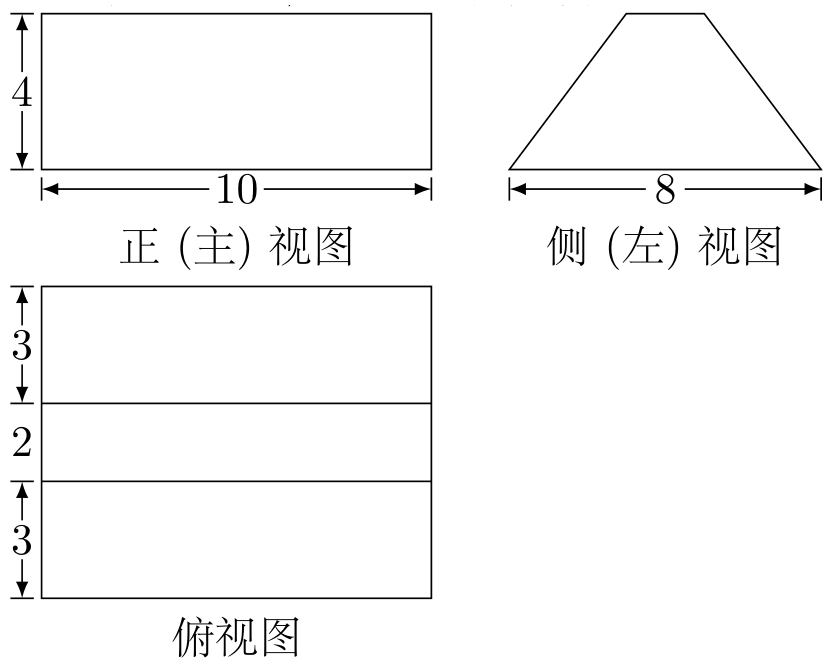
\includegraphics[width=8.2cm]{GaoKao/images/2013/chongqing_liberal/q8_fig1.png}
\end{center}

（\quad）

        {\centering\begin{tabular*}{\linewidth}{@{}@{\extracolsep{\fill}}llll@{}}
          \text{A. }\(180\)  &  \text{B. }\(200\)  &  \text{C. }\(220\)  &  \text{D. }\(240\)
        \end{tabular*}\par}

        \item 已知函数 \( f(x) = ax^3 + b\sin x + 4 \) （\(a, b \in \mathbb{R}\)），\( f(\lg (\log_2 10)) = 5 \)，则 \( f(\lg (\lg 2)) = \)（\quad）

        {\centering\begin{tabular*}{\linewidth}{@{}@{\extracolsep{\fill}}llll@{}}
          \text{A. }\(-5\)  &  \text{B. }\(-1\)  &  \text{C. }\(3\)  &  \text{D. }\(4\)
        \end{tabular*}\par}

        \item 设双曲线 \(C\) 的中心为点 \(O\)，若有且只有一对相交于点 \(O\)，所成的角为 \(60^{\circ}\) 的直线 \(A_{1}B_{1}\) 和 \(A_{2}B_{2}\)，使 \(|A_{1}B_{1}| = |A_{2}B_{2}|\)，其中 \(A_{1}\)，\(B_{1}\) 和 \(A_{2}\)，\(B_{2}\) 分别是这对直线与双曲线 \(C\) 的交点，则该双曲线的离心率的取值范围是（\quad）

        {\centering\begin{tabular*}{\linewidth}{@{}@{\extracolsep{\fill}}llll@{}}
          \text{A. }\(\left(\frac{2\sqrt{3}}{3},2\right]\)  &  \text{B. }\(\left[\frac{2\sqrt{3}}{3},2\right)\)  &  \text{C. }\(\left(\frac{2\sqrt{3}}{3},+\infty\right)\)  &  \text{D. }\(\left[\frac{2\sqrt{3}}{3},+\infty\right)\)
        \end{tabular*}\par}

    \end{enumerate}

\end{description}

\begin{description}

    \item[二、填空题]

    \begin{enumerate}[leftmargin=5pt]

      \addtocounter{enumi}{+10}

        \item 设复数 \(z = 1 + 2\i\) （\(\i\) 是虚数单位），则 \(|z| =\rule[-0.3ex]{3em}{0.4pt}\).

        \item 若 \(2\)，\(a\)，\(b\)，\(c\)，\(9\) 成等差数列，则 \(c - a =\rule[-0.3ex]{3em}{0.4pt}\).

        \item 若甲，乙，丙三人随机地站成一排，则甲，乙两人相邻而站的概率为\rule[-0.3ex]{3em}{0.4pt}.

        \item 在 \(OA\) 为边，\(OB\) 为对角线的矩形中，已知 \(\overrightarrow{OA} = (-3, 1)\)，\(\overrightarrow{OB} = (-2, k)\)，则实数 \(k = \)\rule[-0.3ex]{3em}{0.4pt}.

        \item 设 \(0 \leqslant \alpha \leqslant \pi\)，不等式 \(8x^{2} - (8\sin \alpha)x + \cos 2\alpha \geqslant 0\) 对 \(x \in \mathbb{R}\) 恒成立，则 \(\alpha\) 的取值范围为\rule[-0.3ex]{3em}{0.4pt}.

    \end{enumerate}

\end{description}

\begin{description}

    \item[三、解答题]

    \begin{enumerate}[leftmargin=5pt]

      \addtocounter{enumi}{+15}

        \item 设数列 \(\{a_{n}\}\) 满足：\(a_{1} = 1\)，\(a_{n+1} = 3a_{n}\)，\(n \in \mathbf{N}_{+}\).
\begin{enumerate}
\item 求 \( \{a_{n}\} \) 的通项公式及前 \(n\) 项和 \( S_{n} \)；
\item 已知 \( \{b_{n}\} \) 是等差数列，\( T_{n} \) 为其前 \(n\) 项和，且 \(b_{1}=a_{2}\)，\(b_{3}=a_{1}+a_{2}+a_{3}\)，求 \(T_{20}\).
\end{enumerate}

        \item 从某居民区随机抽取 \(10\text{ 个}\)家庭，获得第 \(i\) 个家庭的月收入 \(x_{i}\) （单位：\(\text{千元}\)）与月储蓄 \(y_{i}\) （单位：\(\text{千元}\)）的数据资料，算得 \(\sum_{i=1}^{10} x_{i} = 80\)，\(\qquad \sum_{i=1}^{10} y_{i} = 20\)，\(\qquad \sum_{i=1}^{10} x_{i}y_{i} = 184\)，\(\qquad \sum_{i=1}^{10} x_{i}^{2} = 720.\)
\begin{enumerate}
\item 求家庭的月储蓄 \(y\) 对月收入 \(x\) 的线性回归方程 \(y = bx + a\)；
\item 判断变量 \(x\) 与 \(y\) 之间是正相关还是负相关；
\item 若该居民区某家庭月收入为 \(7\text{ 千元}\)，预测该家庭的月储蓄.
\end{enumerate}
附：线性回归方程 \(y = bx + a\) 中， \(b = \frac{\sum_{i=1}^{n} x_{i}y_{i} - n\overline{x}\,\overline{y}}{\sum_{i=1}^{n} x_{i}^{2} - n\overline{x}^{2}},\qquad a = \overline{y} - b\overline{x}\)，
其中 \(\overline{x}\)，\(\overline{y}\) 为样本平均值，线性回归方程也可写为 \(\hat{y} = \hat{b}x + \hat{a}\).

        \item 在 \(\triangle ABC\) 中，内角 \(A\)，\(B\)，\(C\) 的对边分别为 \(a\)，\(b\)，\(c\)，且 \(a^2 = b^2 + c^2 + \sqrt{3}bc\).
\begin{enumerate}
\item 求 \(A\)；
\item 设 \(a = \sqrt{3}\)，\(S\) 为 \(\triangle ABC\) 的面积，求 \(S + 3\cos B\cos C\) 的最大值. 并指出此时 \(B\) 的值.
\end{enumerate}

        \item 如图，四棱锥 \(P - ABCD\) 中，\(PA \perp\) 底面 \(ABCD\)，\(PA = 2\sqrt{3}\)，\(BC = CD = 2\)，\(\angle ACB = \angle ACD = \frac{\pi}{3}\).
\begin{enumerate}
\item 求证： \( BD \perp \) 平面 PAC；
\item 若侧棱 \(PC\) 上的点 \(F\) 满足 \(PF = 7FC\)，求三棱锥 \(P - BDF\) 的体积.
\end{enumerate}

\begin{center}
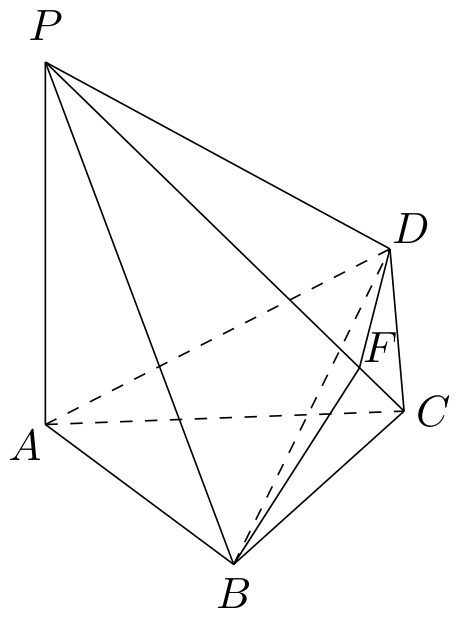
\includegraphics[width=5.7cm]{GaoKao/images/2013/chongqing_liberal/q19_fig1.png}
\end{center}

        \item 某村庄拟修建一个无盖的圆柱形蓄水池（不计厚度）. 设该蓄水池的底面半径为 \(r\text{ 米}\)，高为 \(h\text{ 米}\)，体积为 \(V\text{ 立方米}\). 假设建造成本仅与表面积有关，侧面的建造成本为 \(100\text{ 元/平方米}\)，底面的建造成本为 \(160\text{ 元/平方米}\)，该蓄水池的总建造成本为 \(12000\pi\text{ 元}\)（\(\pi\) 为圆周率）.
\begin{enumerate}
\item 将 \(V\) 表示成 \( r \) 的函数 \( V(r) \)，并求该函数的定义域.
\item 讨论函数 \( V(r) \) 的单调性，并确定 \(r\) 和 \(h\) 为何值时该蓄水池的体积最大.
\end{enumerate}

        \item 如图，椭圆的中心为原点 \(O\)，长轴在 \(x\) 轴上，离心率 \(e = \frac{\sqrt{2}}{2}\)，过左焦点 \(F_{1}\) 作 \(x\) 轴的垂线交椭圆于 \(A\)，\(A'\) 两点，\(|AA'| = 4\).

\begin{enumerate}
\item 求该椭圆的标准方程；
\item 取平行于 \(y\) 轴的直线与椭圆相交于不同的两点 \(P\)，\(P'\)，过 \(P\)，\(P'\) 作圆心为 \(Q\) 的圆，使椭圆上的其余点均在圆 \(Q\) 外，求 \(\triangle PP'Q\) 的面积 \(S\) 的最大值，并写出对应的圆 \(Q\) 的标准方程.
\end{enumerate}

\begin{center}
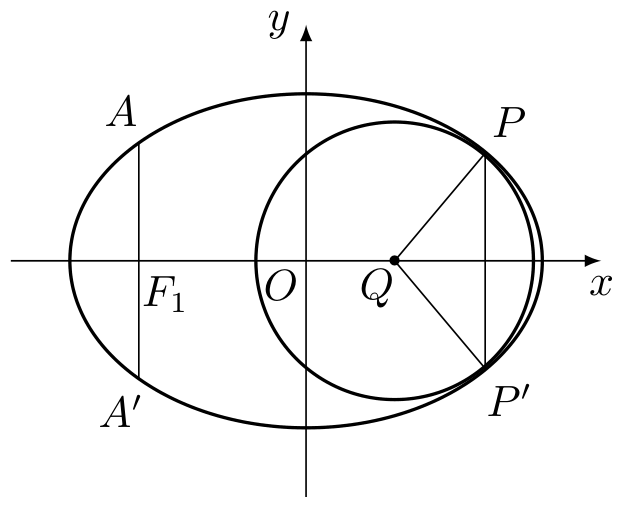
\includegraphics[width=5.7cm]{GaoKao/images/2013/chongqing_liberal/q21_fig1.png}
\end{center}

    \end{enumerate}

\end{description}


\subsection{2013年福建卷（理）}\label{gk:2013年福建卷（理）}

\begin{description}

    \item[一、选择题]

    \begin{enumerate}[leftmargin=5pt]

        \item 已知复数 \(\overline{z} = 1 + 2\i\)（\(\i\)为虚数单位），则 \(z\) 在复平面内对应的点位于（\quad）

        {\centering\begin{tabular*}{\linewidth}{@{}@{\extracolsep{\fill}}llll@{}}
          \text{A. }第一象限  &  \text{B. }第二象限  &  \text{C. }第三象限  &  \text{D. }第四象限
        \end{tabular*}\par}

        \item 已知集合 \(A = \{1, a\}\)，\(B = \{1, 2, 3\}\)，则“\(a = 3\)”是“\(A \subseteq B\)”的（\quad）

        {\centering\begin{tabular*}{\linewidth}{@{}@{\extracolsep{\fill}}llll@{}}
          \text{A. }充分而不必要条件  &  \text{B. }必要而不充分条件  &  \text{C. }充分必要条件  &  \text{D. }既不充分也不必要条件
        \end{tabular*}\par}

        \item 双曲线 \(\frac{x^{2}}{4} - y^{2} = 1\) 的顶点到渐近线的距离等于（\quad）

        {\centering\begin{tabular*}{\linewidth}{@{}@{\extracolsep{\fill}}llll@{}}
          \text{A. }\(\frac{2}{5}\)  &  \text{B. }\(\frac{4}{5}\)  &  \text{C. }\(\frac{2\sqrt{5}}{5}\)  &  \text{D. }\(\frac{4\sqrt{5}}{5}\)
        \end{tabular*}\par}

        \item 某校从高一年级学生中随机抽取部分学生，将他们的模块测试成绩分成 \(6\) 组：\([40,50)\)，\([50,60)\)，\([60,70)\)，\([70,80)\)，\([80,90)\)，\([90,100)\) 加以统计，得到如图所示的频率分布直方图. 已知高一年级共有学生 \(600\) 名，据此估计，该模块测试成绩不少于 \(60\) 分的学生人数为（\quad）

\begin{center}
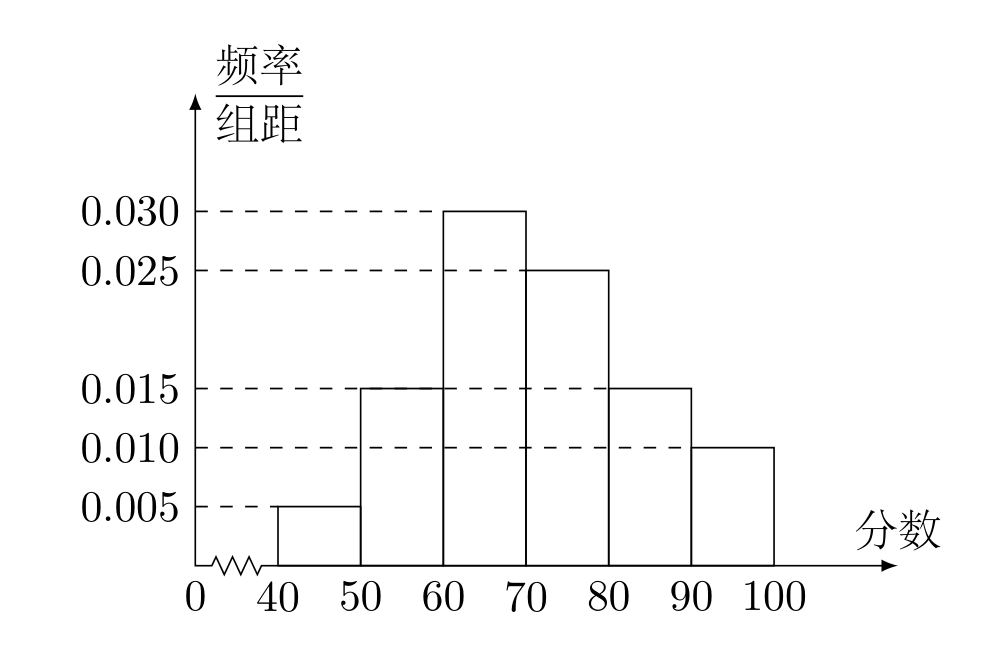
\includegraphics[width=0.92\linewidth]{GaoKao/images/2013/fujian_science/q4_fig1.png}
\end{center}

        {\centering\begin{tabular*}{\linewidth}{@{}@{\extracolsep{\fill}}llll@{}}
          \text{A. }588  &  \text{B. }480  &  \text{C. }450  &  \text{D. }120
        \end{tabular*}\par}

        \item 满足 \(a,b \in \{-1, 0, 1, 2\}\)，且关于 \(x\) 的方程 \(ax^{2} + 2x + b = 0\) 有实数解的有序数对 \((a, b)\) 的个数为（\quad）

        {\centering\begin{tabular*}{\linewidth}{@{}@{\extracolsep{\fill}}llll@{}}
          \text{A. }14  &  \text{B. }13  &  \text{C. }12  &  \text{D. }10
        \end{tabular*}\par}

        \item 阅读如图所示的程序框图，若输入的 \(k = 10\)，则该算法的功能是（\quad）

\begin{center}
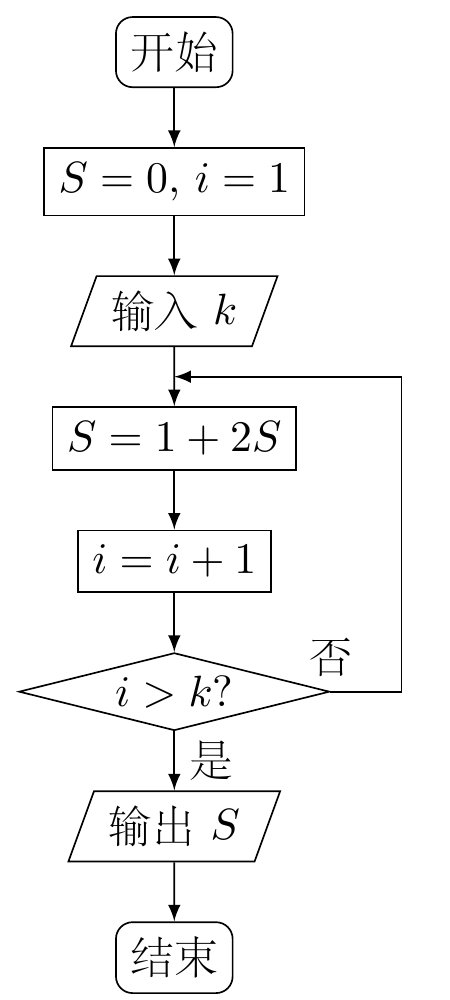
\includegraphics[width=0.30\linewidth]{GaoKao/images/2013/fujian_science/q6_fig1.png}
\end{center}

        {\centering\begin{tabular*}{\linewidth}{@{}@{\extracolsep{\fill}}llll@{}}
          \text{A. }计算数列 \(\{2^{n-1}\}\) 的前 \(10\) 项和  &  \text{B. }计算数列 \(\{2^{n-1}\}\) 的前 \(9\) 项和  &  \text{C. }计算数列 \(\{2^{n}-1\}\) 的前 \(10\) 项和  &  \text{D. }计算数列 \(\{2^{n}-1\}\) 的前 \(9\) 项和
        \end{tabular*}\par}

        \item 在四边形 \(ABCD\) 中，\(\overrightarrow{AC} = (1, 2)\)，\(\overrightarrow{BD} = (-4, 2)\)，则该四边形的面积为（\quad）

        {\centering\begin{tabular*}{\linewidth}{@{}@{\extracolsep{\fill}}llll@{}}
          \text{A. }\(\sqrt{5}\)  &  \text{B. }\(2\sqrt{5}\)  &  \text{C. }5  &  \text{D. }10
        \end{tabular*}\par}

        \item 设函数 \(f(x)\) 的定义域为 \(\mathbb{R}\)，\(x_0\)（\(x_0 \neq 0\)）是 \(f(x)\) 的极大值点，以下结论一定正确的是（\quad）

        {\centering\begin{tabular*}{\linewidth}{@{}@{\extracolsep{\fill}}llll@{}}
          \text{A. }\(\forall x \in \mathbb{R},\, f(x) \leqslant f(x_0)\)  &  \text{B. }\(-x_0\) 是 \(f(-x)\) 的极小值点  &  \text{C. }\(-x_0\) 是 \(-f(x)\) 的极小值点  &  \text{D. }\(-x_0\) 是 \(-f(-x)\) 的极小值点
        \end{tabular*}\par}

        \item 已知等比数列 \(\{a_n\}\) 的公比为 \(q\)，记 \(b_n = a_{m(n-1)+1} + a_{m(n-1)+2} + \cdots + a_{m(n-1)+m}\)，\(c_n = a_{m(n-1)+1} \cdot a_{m(n-1)+2} \cdot \cdots \cdot a_{m(n-1)+m}\)
（\(m, n \in \mathbb{N}^{*}\)），则以下结论一定正确的是（\quad）

        {\centering\begin{tabular*}{\linewidth}{@{}@{\extracolsep{\fill}}llll@{}}
          \text{A. }数列 \(\{b_n\}\) 为等差数列，公差为 \(q^{m}\)  &  \text{B. }数列 \(\{b_n\}\) 为等比数列，公比为 \(q^{2m}\)  &  \text{C. }数列 \(\{c_n\}\) 为等比数列，公比为 \(q^{m^{2}}\)  &  \text{D. }数列 \(\{c_n\}\) 为等比数列，公比为 \(q^{m^{m}}\)
        \end{tabular*}\par}

        \item 设 \(S\)，\(T\) 是 \(\mathbb{R}\) 的两个非空子集，如果存在一个从 \(S\) 到 \(T\) 的函数 \(y = f(x)\) 满足：
\begin{enumerate}
\item \(T = \{f(x) \mid x \in S\}\)；
\item 对任意 \(x_1\)，\(x_2 \in S\)，当 \(x_1 < x_2\) 时，恒有 \(f(x_1) < f(x_2)\).
\end{enumerate}
那么称这两个集合“保序同构”，以下集合对不是“保序同构”的是（\quad）

        {\centering\begin{tabular*}{\linewidth}{@{}@{\extracolsep{\fill}}llll@{}}
          \text{A. }\(A = \mathbb{N}^{*},\ B = \mathbb{N}\)  &  \text{B. }\(A = \{x \mid -1 \leqslant x \leqslant 3\}\)，\(\ B = \{x \mid x = -8 \text{\ 或\ } 0 < x \leqslant 10\}\)  &  \text{C. }\(A = \{x \mid 0 < x < 1\}\)，\(\ B = \mathbb{R}\)  &  \text{D. }\(A = \mathbb{Z}\)，\(\ B = \mathbb{Q}\)
        \end{tabular*}\par}

    \end{enumerate}

\end{description}

\begin{description}

    \item[二、填空题]

    \begin{enumerate}[leftmargin=5pt]

      \addtocounter{enumi}{+10}

        \item 利用计算机产生 \(0 \sim 1\) 之间的均匀随机数 \(a\)，则事件“\(3a - 1 > 0\)”发生的概率为\rule[-0.3ex]{3em}{0.4pt}.

        \item 已知某一多面体内接于球构成一个简单组合体，如果该组合体的正视图，侧视图，俯视图均如图所示，且图中的四边形是边长为 \(2\) 的正方形，则该球的表面积是\rule[-0.3ex]{3em}{0.4pt}.

\begin{center}
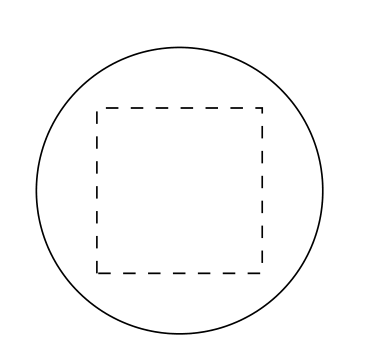
\includegraphics[width=5.5cm]{GaoKao/images/2013/fujian_science/q12_fig1.png}
\end{center}

        \item 如图，在 \(\triangle ABC\) 中，已知点 \(D\) 在 \(BC\) 边上，\(AD \perp AC\)，\(\sin \angle BAC = \frac{2\sqrt{2}}{3}\)，\(AB = 3\sqrt{2}\)，\(AD = 3\)，则 \(BD\) 的长为\rule[-0.3ex]{3em}{0.4pt}.

\begin{center}
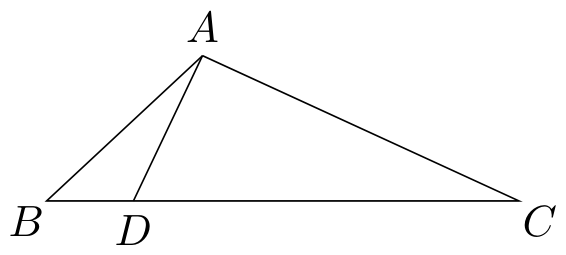
\includegraphics[width=6.6cm]{GaoKao/images/2013/fujian_science/q13_fig1.png}
\end{center}

        \item 椭圆 \(\Gamma : \frac{x^{2}}{a^{2}} + \frac{y^{2}}{b^{2}} = 1\)（\(a > b > 0\)）的左右焦点分别为 \(F_1\)，\(F_2\)，焦距为 \(2c\)，若直线 \(y = \sqrt{3}(x + c)\) 与椭圆 \(\Gamma\) 的一个交点 \(M\) 满足 \(\angle MF_1F_2 = 2 \angle MF_2F_1\)，则该椭圆的离心率等于\rule[-0.3ex]{3em}{0.4pt}.

        \item 当 \(x \in \mathbb{R}\)，\(|x| < 1\) 时，有如下表达式： \(1 + x + x^{2} + \cdots + x^{n} + \cdots = \frac{1}{1-x}.\)
两边同时积分得： \(\int_{0}^{\frac{1}{2}} 1\,\text{d}x + \int_{0}^{\frac{1}{2}} x\,\text{d}x + \int_{0}^{\frac{1}{2}} x^{2}\,\text{d}x + \cdots + \int_{0}^{\frac{1}{2}} x^{n}\,\text{d}x + \cdots = \int_{0}^{\frac{1}{2}} \frac{1}{1-x}\,\text{d}x\)，
从而得到如下等式： \(1 \times \frac{1}{2} + \frac{1}{2} \times \left(\frac{1}{2}\right)^{2} + \frac{1}{3} \times \left(\frac{1}{2}\right)^{3} + \cdots + \frac{1}{n+1} \times \left(\frac{1}{2}\right)^{n+1} + \cdots = \ln 2.\)
请根据以上材料所蕴含的数学思想方法，计算： \(\mathrm C_{n}^{0} \times \frac{1}{2} + \frac{1}{2} \mathrm C_{n}^{1} \times \left(\frac{1}{2}\right)^{2} + \frac{1}{3} \mathrm C_{n}^{2} \times \left(\frac{1}{2}\right)^{3} + \cdots + \frac{1}{n+1} \mathrm C_{n}^{n} \times \left(\frac{1}{2}\right)^{n+1} =\rule[-0.3ex]{3em}{0.4pt}.\)

    \end{enumerate}

\end{description}

\begin{description}

    \item[三、解答题]

    \begin{enumerate}[leftmargin=5pt]

      \addtocounter{enumi}{+15}

        \item 某联欢晚会举行抽奖活动，举办方设置了甲，乙两种抽奖方案，方案甲的中奖率为 \(\frac{2}{3}\)，中奖可以获得 \(2\) 分；方案乙的中奖率为 \(\frac{2}{5}\)，中奖可以获得 \(3\) 分；未中奖则不得分. 每人有且只有一次抽奖机会，每次抽奖中奖与否互不影响，晚会结束后凭分数兑换奖品.

\begin{enumerate}
\item 若小明选择方案甲抽奖，小红选择方案乙抽奖，记他们的累计得分为 \(X\)，求 \(X \leqslant 3\) 的概率；
\item 若小明，小红两人都选择方案甲或都选择方案乙进行抽奖，问：他们选择何种方案抽奖，累计得分的数学期望较大？
\end{enumerate}

        \item 已知函数 \(f(x) = x - a \ln x\)（\(a \in \mathbb{R}\)）.

\begin{enumerate}
\item 当 \(a = 2\) 时，求曲线 \(y = f(x)\) 在点 \(A(1, f(1))\) 处的切线方程；
\item 求函数 \(f(x)\) 的极值.
\end{enumerate}

        \item 如图，在正方形 \(OABC\) 中，\(O\) 为坐标原点，点 \(A\) 的坐标为 \((10,0)\)，点 \(C\) 的坐标为 \((0,10)\). 分别将线段 \(OA\) 和 \(AB\) 十等分，分点分别记为 \(A_1\)，\(A_2\)，\(\cdots\)，\(A_9\) 和 \(B_1\)，\(B_2\)，\(\cdots\)，\(B_9\)，连接 \(OB_i\)，过 \(A_i\) 作 \(x\) 轴的垂线与 \(OB_i\) 交于点 \(P_i\)（\(i \in \mathbb{N}^{*}\)，\(1 \leqslant i \leqslant 9\)）.

\begin{enumerate}
\item 求证：点 \(P_i\)（\(i \in \mathbb{N}^{*}\)，\(1 \leqslant i \leqslant 9\)）都在同一条抛物线上，并求该抛物线 \(E\) 的方程；
\item 过点 \(C\) 作直线 \(l\) 与抛物线 \(E\) 交于不同的两点 \(M\)，\(N\)，若 \(\triangle OCM\) 与 \(\triangle OCN\) 的面积之比为 \(4 : 1\)，求直线 \(l\) 的方程.
\end{enumerate}

\begin{center}
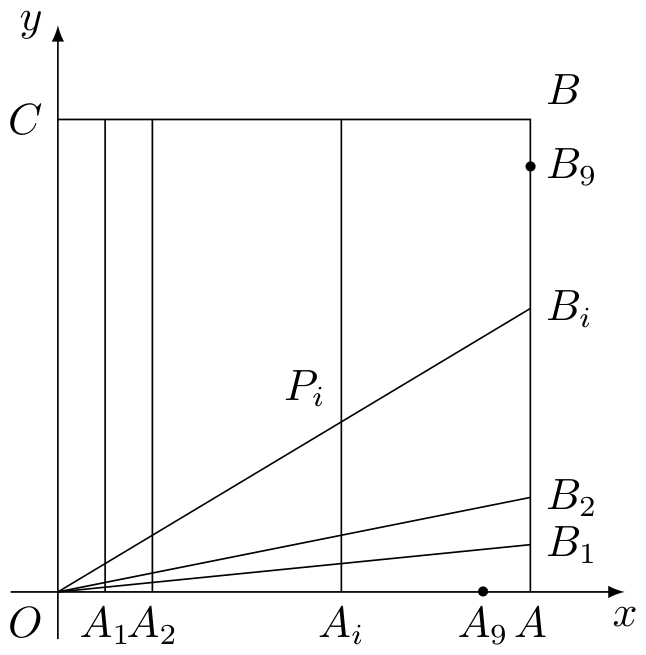
\includegraphics[width=6.4cm]{GaoKao/images/2013/fujian_science/q18_fig1.png}
\end{center}

        \item 如图，在四棱柱 \(ABCD - A_1B_1C_1D_1\) 中，侧棱 \(AA_1 \perp\) 底面 \(ABCD\)，\(AB \parallel DC\)，\(AA_1 = 1\)，\(AB = 3k\)，\(AD = 4k\)，\(BC = 5k\)，\(DC = 6k\)（\(k > 0\)）.

\begin{enumerate}
\item 求证：\(CD \perp\) 平面 \(ADD_1A_1\)；
\item 若直线 \(AA_1\) 与平面 \(AB_1C\) 所成的正弦值为 \(\frac{6}{7}\)，求 \(k\) 的值；
\item 现将与四棱柱 \(ABCD - A_1B_1C_1D_1\) 形状和大小完全相同的两个四棱柱拼成一个新的四棱柱，规定：若拼成的新四棱柱形状和大小完全相同，则视为一种拼接方案，问：共有几种不同的拼接方案？在这些拼接成的新四棱柱中，记其中最小的表面积为 \(f(k)\)，写出 \(f(k)\) 的解析式.（直接写出答案，不必说明理由）
\end{enumerate}

\begin{center}
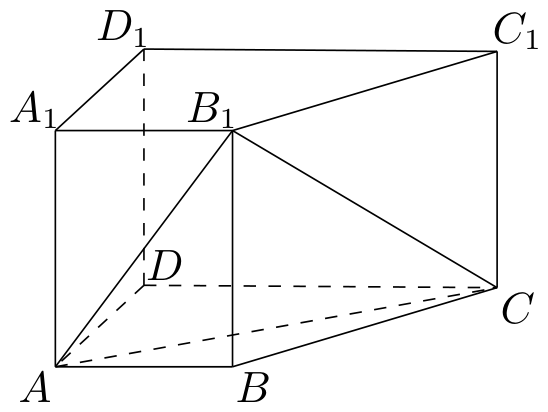
\includegraphics[width=5.7cm]{GaoKao/images/2013/fujian_science/q19_fig1.png}
\end{center}

        \item 已知函数 \(f(x) = \sin(\omega x + \varphi)\)（\(\omega > 0\)，\(\ 0 < \varphi < \pi\)）的周期为 \(\pi\)，图象的一个对称中心为 \(\left(\frac{\pi}{4}, 0\right)\)，将函数 \(f(x)\) 图象上所有点的横坐标伸长到原来的 \(2\) 倍（纵坐标不变），再将得到的图象向右平移 \(\frac{\pi}{2}\) 个单位长度后得到函数 \(g(x)\) 的图象.

\begin{enumerate}
\item 求函数 \(f(x)\) 与 \(g(x)\) 的解析式；
\item 是否存在 \(x_0 \in \left(\frac{\pi}{6}, \frac{\pi}{4}\right)\)，使得 \(f(x_0)\)，\(g(x_0)\)，\(f(x_0)g(x_0)\) 按照某种顺序成等差数列？若存在，请确定 \(x_0\) 的个数；若不存在，说明理由；
\item 求实数 \(a\) 与正整数 \(n\)，使得 \(F(x) = f(x) + a g(x)\) 在 \((0, n\pi)\) 内恰有 \(2013\) 个零点.
\end{enumerate}

    \end{enumerate}

\end{description}

\begin{description}

    \item[四、选考题]

    \begin{enumerate}[leftmargin=5pt]

      \addtocounter{enumi}{+20}

        \item 已知直线 \(l: ax + y = 1\) 在矩阵 \(A = \begin{pmatrix}1 & 2 \\ 0 & 1\end{pmatrix}\) 对应的变换作用下变为直线 \(l': x + by = 1\).

\begin{enumerate}
\item 求实数 \(a\)，\(b\) 的值；
\item 若点 \(P(x_0, y_0)\) 在直线 \(l\) 上，且 \(A \begin{pmatrix}x_0 \\ y_0\end{pmatrix} = \begin{pmatrix}x_0 \\ y_0\end{pmatrix}\)，求点 \(P\) 的坐标.
\end{enumerate}

        \item \textbf{【选修4-4：坐标系与参数方程】}

在平面直角坐标系中，以坐标原点为极点，\(x\) 轴的正半轴为极轴建立极坐标系.已知点 \(A\) 的极坐标为 \(\left(\sqrt{2}, \frac{\pi}{4}\right)\)，直线 \(l\) 的极坐标方程为 \(\rho \cos \left(\theta - \frac{\pi}{4}\right) = a\)，且点 \(A\) 在直线 \(l\) 上.

\begin{enumerate}
\item 求 \(a\) 的值及直线 \(l\) 的直角坐标方程；
\item 圆 \(C\) 的参数方程为 \(\begin{cases}
x = 1 + \cos \alpha,\\
y = \sin \alpha,
\end{cases}\)（\(\alpha\) 为参数），试判断直线 \(l\) 与圆 \(C\) 的位置关系.
\end{enumerate}

        \item \textbf{【选修4-5：不等式选讲】}

设不等式 \(|x - 2| < a\)（\(a \in \mathbb{N}^{*}\)）的解集为 \(A\)，且 \(\frac{3}{2} \in A\)，\(\ \frac{1}{2} \notin A\).

\begin{enumerate}
\item 求 \(a\) 的值；
\item 求函数 \(f(x) = |x + a| + |x - 2|\) 的最小值.
\end{enumerate}

    \end{enumerate}

\end{description}


\subsection{2013年福建卷（文）}\label{gk:2013年福建卷（文）}

\begin{description}

    \item[一、选择题]

    \begin{enumerate}[leftmargin=5pt]

        \item 复数 \(z = -1 - 2\i\)（\(\i\)为虚数单位）在复平面内对应的点位于（\quad）

        {\centering\begin{tabular*}{\linewidth}{@{}@{\extracolsep{\fill}}llll@{}}
          \text{A. }第一象限  &  \text{B. }第二象限  &  \text{C. }第三象限  &  \text{D. }第四象限
        \end{tabular*}\par}

        \item 设点 \(P(x, y)\)，则“\(x = 2\) 且 \(y = -1\)”是“点 \(P\) 在直线 \(l: x + y - 1 = 0\) 上”的（\quad）

        {\centering\begin{tabular*}{\linewidth}{@{}@{\extracolsep{\fill}}llll@{}}
          \text{A. }充分而不必要条件  &  \text{B. }必要而不充分条件  &  \text{C. }充分必要条件  &  \text{D. }既不充分也不必要条件
        \end{tabular*}\par}

        \item 若集合 \(A = \{1, 2, 3\}\)，\(B = \{1, 3, 4\}\)，则 \(A \cap B\) 的子集个数为（\quad）

        {\centering\begin{tabular*}{\linewidth}{@{}@{\extracolsep{\fill}}llll@{}}
          \text{A. }2  &  \text{B. }3  &  \text{C. }4  &  \text{D. }16
        \end{tabular*}\par}

        \item 双曲线 \(x^{2} - y^{2} = 1\) 的顶点到其渐近线的距离等于（\quad）

        {\centering\begin{tabular*}{\linewidth}{@{}@{\extracolsep{\fill}}llll@{}}
          \text{A. }\(\frac{1}{2}\)  &  \text{B. }\( \frac{\sqrt{2}}{2} \)  &  \text{C. }1  &  \text{D. }\(\sqrt{2}\)
        \end{tabular*}\par}

        \item 函数 \( f(x) = \ln (x^2 + 1) \) 的图象大致是（\quad）

        {\centering\begin{tabular*}{\linewidth}{@{}@{\extracolsep{\fill}}cccc@{}}
          \text{A. }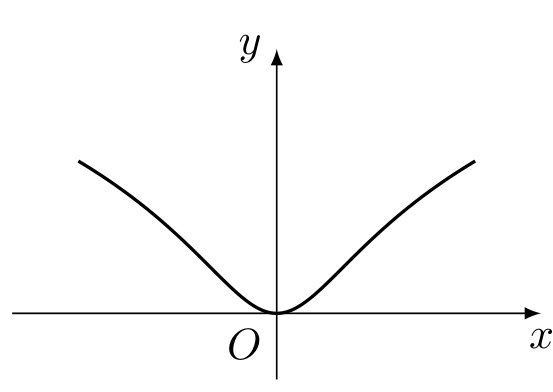
\includegraphics[width=0.15\paperwidth]{GaoKao/images/2013/fujian_liberal/q5_optA.png}  &  \text{B. }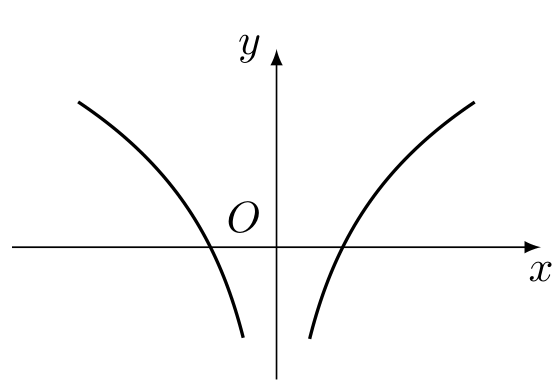
\includegraphics[width=0.15\paperwidth]{GaoKao/images/2013/fujian_liberal/q5_optB.png}  &  \text{C. }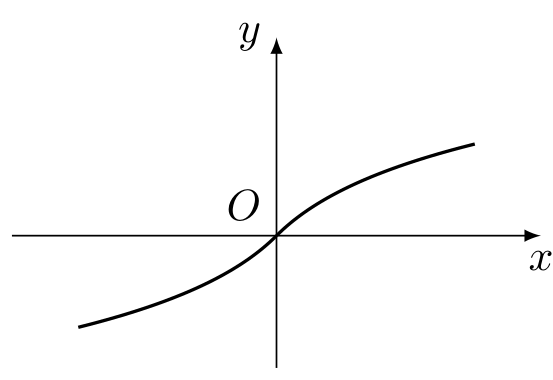
\includegraphics[width=0.15\paperwidth]{GaoKao/images/2013/fujian_liberal/q5_optC.png}  &  \text{D. }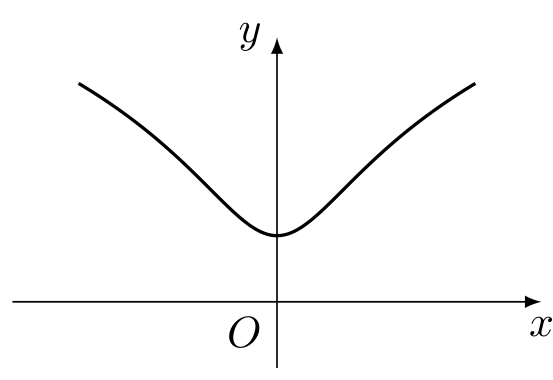
\includegraphics[width=0.15\paperwidth]{GaoKao/images/2013/fujian_liberal/q5_optD.png}
        \end{tabular*}\par}

        \item 若变量 \(x\)，\(y\) 满足约束条件 \(\begin{cases}
x + y \leqslant 2,\\
x \geqslant 1,\\
y \geqslant 0,
\end{cases}\) 则 \(z = 2x + y\) 的最大值和最小值分别为（\quad）

        {\centering\begin{tabular*}{\linewidth}{@{}@{\extracolsep{\fill}}llll@{}}
          \text{A. }4 和 3  &  \text{B. }4 和 2  &  \text{C. }3 和 2  &  \text{D. }2 和 0
        \end{tabular*}\par}

        \item 若 \(2^{x} + 2^{y} = 1\)，则 \(x + y\) 的取值范围是（\quad）

        {\centering\begin{tabular*}{\linewidth}{@{}@{\extracolsep{\fill}}llll@{}}
          \text{A. }[0,2]  &  \text{B. }\([-2,0]\)  &  \text{C. }\([-2, +\infty)\)  &  \text{D. }\((- \infty, -2]\)
        \end{tabular*}\par}

        \item 阅读如图所示的程序框图，运行相应的程序，如果输入某个正整数 \(n\) 后，输出的 \(S \in (10, 20)\)，那么 \(n\) 的值为（\quad）

\begin{center}
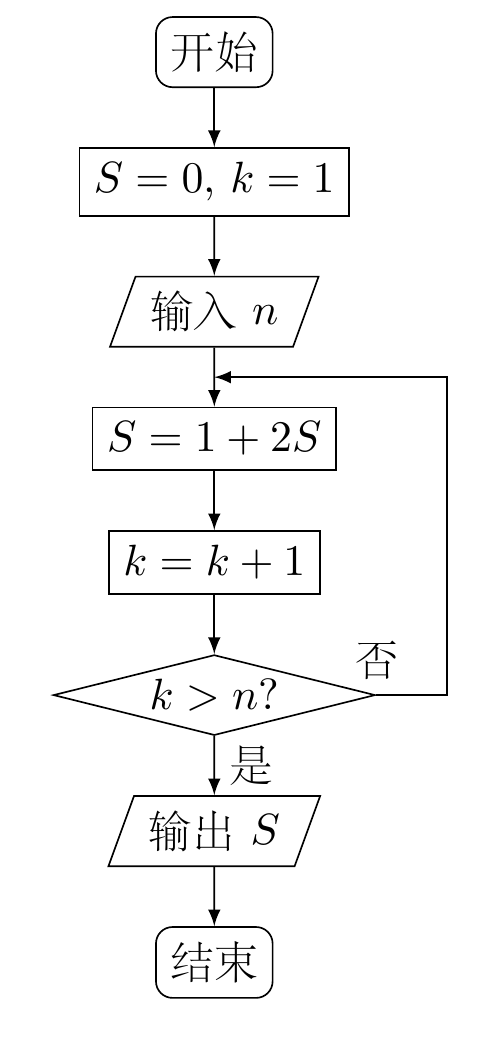
\includegraphics[width=0.30\linewidth]{GaoKao/images/2013/fujian_liberal/q8_fig1.png}
\end{center}

        {\centering\begin{tabular*}{\linewidth}{@{}@{\extracolsep{\fill}}llll@{}}
          \text{A. }3  &  \text{B. }4  &  \text{C. }5  &  \text{D. }6
        \end{tabular*}\par}

        \item 将函数 \( f(x) = \sin (2x + \theta)\)（\(-\frac{\pi}{2} < \theta < \frac{\pi}{2}\)）的图象向右平移 \(\varphi\)（\(\varphi > 0\)）个单位长度后得到函数 \( g(x) \) 的图象. 若 \(f(x)\)，\(g(x)\) 的图象都经过点 \( P\left(0, \frac{\sqrt{3}}{2}\right) \)，则 \(\varphi\) 的值可以是（\quad）

        {\centering\begin{tabular*}{\linewidth}{@{}@{\extracolsep{\fill}}llll@{}}
          \text{A. }\(\frac{5\pi}{3}\)  &  \text{B. }\( \frac{5\pi}{6} \)  &  \text{C. }\( \frac{\pi}{2} \)  &  \text{D. }\(\frac{\pi}{6}\)
        \end{tabular*}\par}

        \item 在四边形 \(ABCD\) 中，\(\overrightarrow{AC} = (1, 2)\)，\(\overrightarrow{BD} = (-4, 2)\)，则该四边形的面积为（\quad）

        {\centering\begin{tabular*}{\linewidth}{@{}@{\extracolsep{\fill}}llll@{}}
          \text{A. }\(\sqrt{5}\)  &  \text{B. }\(2\sqrt{5}\)  &  \text{C. }5  &  \text{D. }10
        \end{tabular*}\par}

        \item 已知 \(x\) 与 \(y\) 之间的几组数据如下表：

\begin{center}
\begin{tabular}{c|cccccc}
\(x\) & \(1\) & \(2\) & \(3\) & \(4\) & \(5\) & \(6\) \\
\hline
\(y\) & \(0\) & \(2\) & \(1\) & \(3\) & \(3\) & \(4\)
\end{tabular}
\end{center}

假设根据上表数据所得线性回归直线方程为 \( \hat{y} = \hat{b}x + \hat{a} \)，若某同学根据上表中的前两组数据 \((1, 0)\) 和 \((2, 2)\) 求得的直线方程为 \( y = b'x + a' \)，则以下结论正确的是（\quad）

        {\centering\begin{tabular*}{\linewidth}{@{}@{\extracolsep{\fill}}llll@{}}
          \text{A. }\(\hat{b} > b', \hat{a} > a'\)  &  \text{B. }\(\hat{b} > b'\)，\(\hat{a} < a'\)  &  \text{C. }\(\hat{b} < b'\)，\(\hat{a} > a'\)  &  \text{D. }\(\hat{b} < b'\)，\(\hat{a} < a'\)
        \end{tabular*}\par}

        \item 设函数 \( f(x) \) 的定义域为 \(\mathbb{R}\)，\(x_0 \) （\(x_0 \neq 0\)）是 \( f(x) \) 的极大值点，以下结论一定正确的是（\quad）

        {\centering\begin{tabular*}{\linewidth}{@{}@{\extracolsep{\fill}}llll@{}}
          \text{A. }\(\forall x\in \mathbb{R},f(x)\leqslant f(x_0)\)  &  \text{B. }\(-x_0\) 是 \(f(-x)\) 的极小值点  &  \text{C. }\(-x_0\) 是 \(-f(x)\) 的极小值点  &  \text{D. }\(-x_0\) 是 \(-f(-x)\) 的极小值点
        \end{tabular*}\par}

    \end{enumerate}

\end{description}

\begin{description}

    \item[二、填空题]

    \begin{enumerate}[leftmargin=5pt]

      \addtocounter{enumi}{+12}

        \item 已知函数 \(f(x) = \begin{cases}
2x^{3}, & x < 0,\\
-\tan x, & 0 \leqslant x < \frac{\pi}{2},
\end{cases}\) 则 \(f\left(f\left(\frac{\pi}{4}\right)\right)=\rule[-0.3ex]{3em}{0.4pt}.\)

        \item 利用计算机产生 \(0 \sim 1\) 之间的均匀随机数 \(a\)，则事件“\(3a - 1 < 0\)”发生的概率为\rule[-0.3ex]{3em}{0.4pt}.

        \item 椭圆 \(\Gamma: \frac{x^2}{a^2} + \frac{y^2}{b^2} = 1\)（\(a > b > 0\)）的左右焦点分别为 \(F_1\)，\(F_2\)，焦距为 \(2c\). 若直线 \(y = \sqrt{3}(x + c)\) 与椭圆 \(\Gamma\) 的一个交点 \(M\) 满足 \(\angle MF_1F_2 = 2\angle MF_2F_1\)，则该椭圆的离心率等于\rule[-0.3ex]{3em}{0.4pt}.

        \item 设 \(S\)，\(T\) 是 \(\mathbb{R}\) 的两个非空子集. 如果存在一个从 \(S\) 到 \(T\) 的函数 \(y = f(x)\) 满足：
\begin{enumerate}
\item \(T = \{f(x)\mid x\in S\}\)；
\item 对任意 \(x_{1}\)，\(x_{2} \in S\)，当 \(x_{1} < x_{2}\) 时，恒有 \(f(x_{1}) < f(x_{2})\)，
\end{enumerate}
那么称这两个集合“保序同构”. 现给出以下 3 对集合：
\begin{enumerate}
\item \(A = \mathbb{N}\)，\(B = \mathbb{N}^{*};\)
\item \(A = \{x\mid -1\leqslant x\leqslant 3\}\)，\(B = \{x\mid -8\leqslant x\leqslant 10\}\)；
\item \( A = \{x \mid 0 < x < 1\} \)，\( B = \mathbb{R} \).
\end{enumerate}
其中，“保序同构”的集合对的序号是\rule[-0.3ex]{3em}{0.4pt}. （写出所有“保序同构”的集合对的序号）

    \end{enumerate}

\end{description}

\begin{description}

    \item[三、解答题]

    \begin{enumerate}[leftmargin=5pt]

      \addtocounter{enumi}{+16}

        \item 已知等差数列 \(\{a_{n}\}\) 的公差 \(d = 1\)，前 \(n\) 项和为 \(S_{n}\).
\begin{enumerate}
\item 若 \(1\)，\(a_{1}\)，\(a_{3}\) 成等比数列，求 \(a_{1}\)；
\item 若 \(S_{5} > a_{1}a_{9}\)，求 \(a_{1}\) 的取值范围.
\end{enumerate}

        \item 如图，在四棱锥 \(P-ABCD\) 中，\(PD \perp\) 平面 \(ABCD\)，\(AB \parallel DC\)，\(AB \perp AD\)，\(BC = 5\)，\(DC = 3\)，\(AD = 4\)，\(\angle PAD = 60^\circ\).
\begin{enumerate}
\item 当正视方向与向量 \( \overrightarrow{AD} \) 的方向相同时，画出四棱锥 \(P-ABCD\) 的正视图 （要求标出尺寸，并写出演算过程）；
\item 若 \(M\) 为 \(PA\) 的中点，求证： \(DM \parallel\) 平面 \(PBC\)；
\item 求三棱锥 \(D-PBC\) 的体积.
\end{enumerate}

        \item 某工厂有 25 周岁以上（含 25 周岁）工人 300 名，25 周岁以下工人 200 名. 为研究工人的日平均生产量是否与年龄有关，现采用分层抽样的方法，从中抽取了 100 名工人，先统计了他们某月的日平均生产件数，然后按工人年龄在“25 周岁以上（含 25 周岁）”和“25 周岁以下”分为两组，再将两组工人的日平均生产件数分成 5 组：\([50, 60)\)，\([60, 70)\)，\([70, 80)\)，\([80, 90)\)，\([90, 100]\) 分别加以统计，得到如图所示的频率分布直方图.

\begin{enumerate}
\item 从样本中日平均生产件数不足 60 件的工人中随机抽取 2 人，求至少抽到一名“25 周岁以下组”工人的概率；
\item 规定日平均生产件数不少于 80 件者为“生产能手”，请你根据已知条件完成 \(2\times 2\) 列联表，并判断是否有 \(90\%\) 的把握认为“生产能手与工人所在的年龄组有关”.
\end{enumerate}
附：\(\chi^2 = \frac{n(ad - bc)^2}{(a + b)(c + d)(a + c)(b + d)}\)，\(P\left\{\chi^{2} \geqslant k\right\}\)

\begin{center}
\begin{tabular}{c|cccc}
\(P\{\chi^2 \geqslant k\}\) & \(0.100\) & \(0.050\) & \(0.010\) & \(0.001\) \\
\hline
\(k\) & \(2.706\) & \(3.841\) & \(6.635\) & \(10.828\)
\end{tabular}
\end{center}

（注：此处公式也可以写成 \(K^2 = \frac{n(ad - bc)^2}{(a + b)(c + d)(a + c)(b + d)}\)）

\begingroup
\leftskip=0pt
\rightskip=0pt
\begin{center}
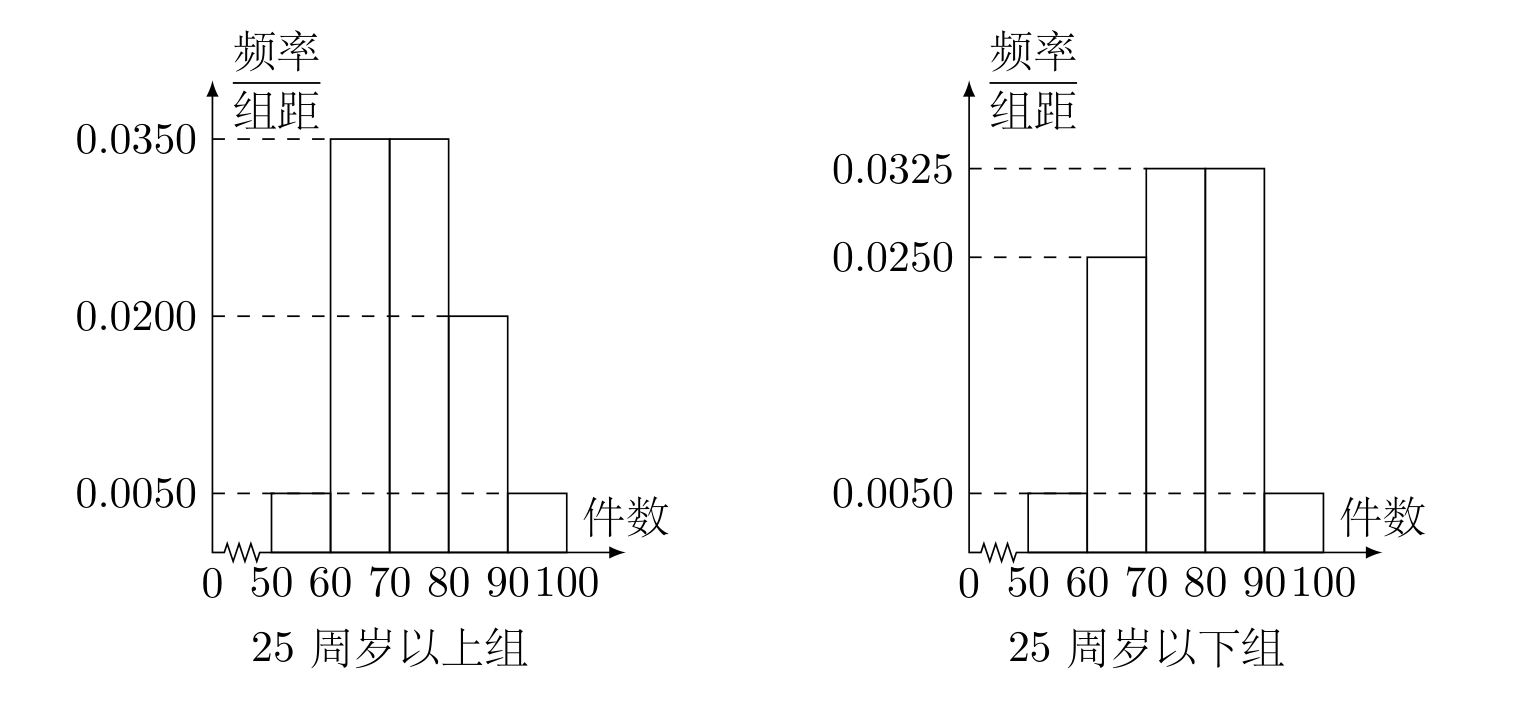
\includegraphics[width=0.92\linewidth]{GaoKao/images/2013/fujian_liberal/q19_fig1.png}
\end{center}
\endgroup

        \item 如图，抛物线 \(E: y^{2} = 4x\) 的焦点为 \(F\)，准线 \(l\) 与 \(x\) 轴的交点为 \(A\). 点 \(C\) 在抛物线 \(E\) 上. 以 \(C\) 为圆心，\(|CO|\) 为半径作圆，设圆 \(C\) 与准线 \(l\) 交于不同的两点 \(M\)，\(N\).
\begin{enumerate}
\item 若点 C 的纵坐标为 2，求 \( \left|MN\right| \)；
\item 若 \( \left|AF\right|^{2}=\left|AM\right|\cdot\left|AN\right| \)，求圆 C 的半径.
\end{enumerate}

\begin{center}
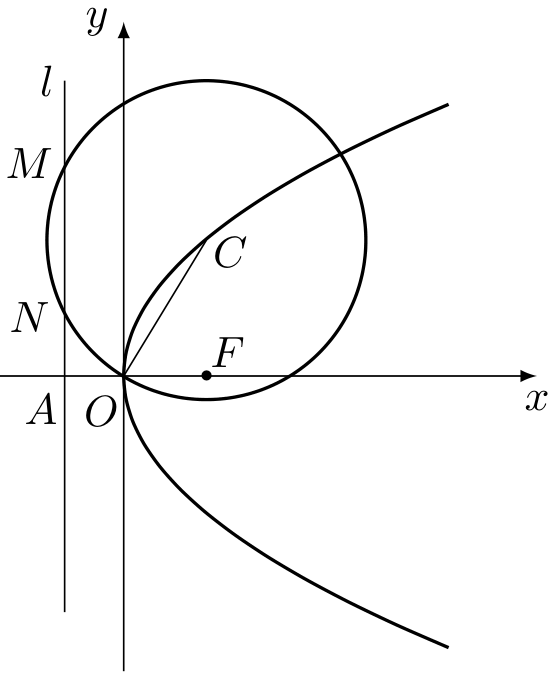
\includegraphics[width=6.7cm]{GaoKao/images/2013/fujian_liberal/q20_fig1.png}
\end{center}

        \item 如图，在等腰直角 \(\triangle OPQ\) 中，\(\angle POQ = 90^{\circ}\)，\(OP = 2\sqrt{2}\)，点 \(M\) 在线段 \(PQ\) 上.
\begin{enumerate}
\item 若 \(OM = \sqrt{5}\)，求 \(PM\) 的长；
\item 若点 \(N\) 在线段 \(MQ\) 上，且 \(\angle MON = 30^{\circ}\)，问：当 \(\angle POM\) 取何值时，\(\triangle OMN\) 的面积最小？ 并求出面积的最小值.
\end{enumerate}

\begin{center}
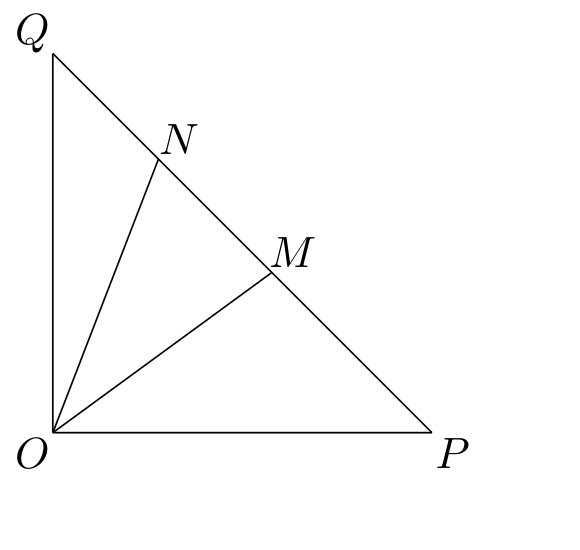
\includegraphics[width=5.0cm]{GaoKao/images/2013/fujian_liberal/q21_fig1.png}
\end{center}

        \item 已知函数 \( f(x) = x - 1 + \frac{a}{e^{x}} \)（\( a \in \mathbb{R} \)，\(e\) 为自然对数的底数）.
\begin{enumerate}
\item 若曲线 \( y = f(x) \) 在点 \( (1, f(1)) \) 处的切线平行于 \( x \) 轴，求 \(a\) 的值；
\item 求函数 \( f(x) \) 的极值；
\item 当 \(a = 1\) 时，若直线 \(l: y = kx - 1\) 与曲线 \(y = f(x)\) 没有公共点，求 \(k\) 的最大值.
\end{enumerate}

    \end{enumerate}

\end{description}


\subsection{2013年广东卷（理）}\label{gk:2013年广东卷（理）}

\begin{description}

    \item[一、选择题]

    \begin{enumerate}[leftmargin=5pt]

        \item 设集合 \(M = \{x \mid x^2 + 2x = 0, x \in \mathbb{R}\}\)，\(N = \{x \mid x^2 - 2x = 0, x \in \mathbb{R}\}\)，则 \(M \cup N =\)（\quad）

        {\centering\begin{tabular*}{\linewidth}{@{}@{\extracolsep{\fill}}llll@{}}
          \text{A. }\( \{0\} \)  &  \text{B. }\( \{0, 2\} \)  &  \text{C. }\(\{-2, 0\}\)  &  \text{D. }\(\{-2, 0, 2\}\)
        \end{tabular*}\par}

        \item 定义域为 \(\mathbb{R}\) 的四个函数 \(y = x^3\)，\(y = 2^x\)，\(y = x^2 + 1\)，\(y = 2\sin x\) 中，奇函数的个数是（\quad）

        {\centering\begin{tabular*}{\linewidth}{@{}@{\extracolsep{\fill}}llll@{}}
          \text{A. }\(4\)  &  \text{B. }\(3\)  &  \text{C. }\(2\)  &  \text{D. }\(1\)
        \end{tabular*}\par}

        \item 若复数 \(z\) 满足 \(\i z = 2 + 4\i\)，则在复平面内，\(z\) 对应的点的坐标是（\quad）

        {\centering\begin{tabular*}{\linewidth}{@{}@{\extracolsep{\fill}}llll@{}}
          \text{A. }\((2,4)\)  &  \text{B. }\((2,-4)\)  &  \text{C. }\((4,-2)\)  &  \text{D. }\((4,2)\)
        \end{tabular*}\par}

        \item 已知离散型随机变量 \(X\) 的分布列为

\begin{center}
\begin{tabular}{c|ccc}
\(X\) & \(1\) & \(2\) & \(3\) \\
\hline
\(P\) & \(\frac{3}{5}\) & \(\frac{3}{10}\) & \(\frac{1}{10}\)
\end{tabular}
\end{center}

则 \(X\) 的数学期望 \(E(X) =\)（\quad）

        {\centering\begin{tabular*}{\linewidth}{@{}@{\extracolsep{\fill}}llll@{}}
          \text{A. }\(\frac{3}{2}\)  &  \text{B. }\(2\)  &  \text{C. }\(\frac{5}{2}\)  &  \text{D. }\(3\)
        \end{tabular*}\par}

        \item 某四棱台的三视图如图所示，则该四棱台的体积是（\quad）

\begin{center}
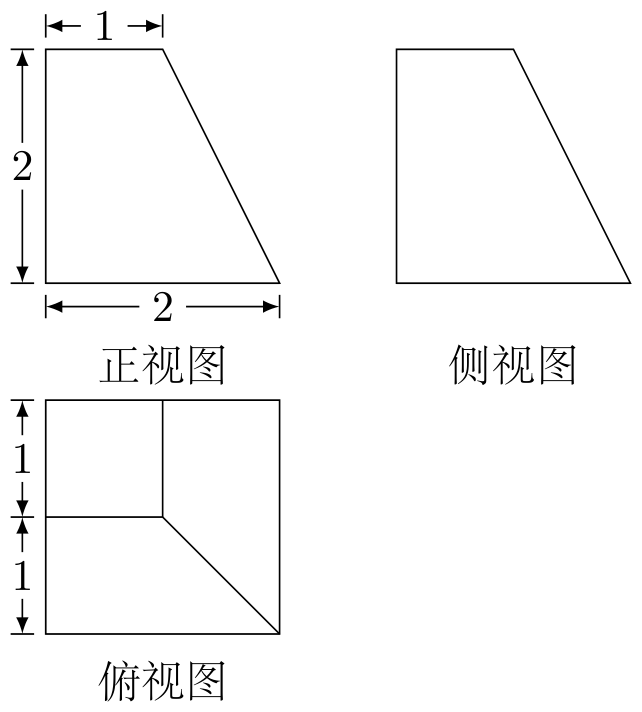
\includegraphics[width=6.3cm]{GaoKao/images/2013/guangdong_science/q5_fig1.png}
\end{center}

        {\centering\begin{tabular*}{\linewidth}{@{}@{\extracolsep{\fill}}llll@{}}
          \text{A. }\(4\)  &  \text{B. }\(\frac{14}{3}\)  &  \text{C. }\(\frac{16}{3}\)  &  \text{D. }\(6\)
        \end{tabular*}\par}

        \item 设 \(m\)，\(n\) 是两条不同的直线，\(\alpha\)，\(\beta\) 是两个不同的平面，下列命题中正确的是（\quad）

        {\centering\begin{tabular*}{\linewidth}{@{}@{\extracolsep{\fill}}llll@{}}
          \text{A. }若 \(\alpha \perp \beta, m \subset \alpha, n \subset \beta\)，则 \(m \perp n\)  &  \text{B. }若 \(\alpha \parallel \beta\)，\(m \subset \alpha\)，\(n \subset \beta\)，则 \(m \parallel n\)  &  \text{C. }若 \(m \perp n\)，\(m \subset \alpha\)，\(n \subset \beta\)，则 \(\alpha \perp \beta\)  &  \text{D. }若 \(m \perp \alpha\)，\(m \parallel n\)，\(n \parallel \beta\)，则 \(\alpha \perp \beta\)
        \end{tabular*}\par}

        \item 已知中心在原点的双曲线 \(C\) 的右焦点为 \(F(3,0)\)，离心率等于 \(\frac{3}{2}\)，则 \(C\) 的方程是（\quad）

        {\centering\begin{tabular*}{\linewidth}{@{}@{\extracolsep{\fill}}llll@{}}
          \text{A. }\(\frac{x^2}{4} -\frac{y^2}{\sqrt{5}} = 1\)  &  \text{B. }\(\frac{x^2}{4} -\frac{y^2}{5} = 1\)  &  \text{C. }\(\frac{x^2}{2} -\frac{y^2}{5} = 1\)  &  \text{D. }\(\frac{x^2}{2} -\frac{y^2}{\sqrt{5}} = 1\)
        \end{tabular*}\par}

        \item 设整数 \(n \geqslant 4\)，集合 \(X = \{1, 2, 3, \cdots, n\}\).
令集合 \(S = \{(x, y, z) \mid x, y, z \in X,\ \text{且三条件 } x < y < z, y < z < x, z < x < y \text{ 恰有一个成立}\}\)，若 \((x, y, z)\) 和 \((z, w, x)\) 都在 \(S\) 中，则下列选项正确的是（\quad）

        {\centering\begin{tabular*}{\linewidth}{@{}@{\extracolsep{\fill}}llll@{}}
          \text{A. }\((y, z, w) \in S, (x, y, w) \notin S\)  &  \text{B. }\((y, z, w) \in S\)，\((x, y, w) \in S\)  &  \text{C. }\((y,z,w)\notin S\)，\((x,y,w)\in S\)  &  \text{D. }\((y,z,w)\notin S\)，\((x,y,w)\notin S\)
        \end{tabular*}\par}

    \end{enumerate}

\end{description}

\begin{description}

    \item[二、填空题]

    \begin{enumerate}[leftmargin=5pt]

      \addtocounter{enumi}{+8}

        \item 不等式 \(x^{2} + x - 2 < 0\) 的解集为\rule[-0.3ex]{3em}{0.4pt}.

        \item 若曲线 \(y = kx + \ln x\) 在点 \((1, k)\) 处的切线平行于 \(x\) 轴，则 \(k=\)\rule[-0.3ex]{3em}{0.4pt}.

        \item 执行如图所示的程序框图，若输入 \(n\) 的值为 \(4\)，则输出 \(s\) 的值为\rule[-0.3ex]{3em}{0.4pt}.

\begin{center}
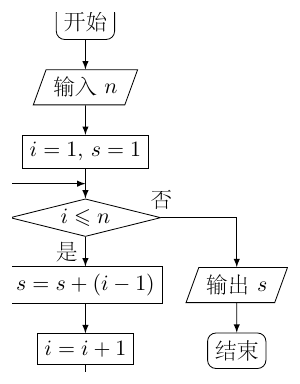
\includegraphics[width=0.34\linewidth]{GaoKao/images/2013/guangdong_science/q11_fig1.png}
\end{center}

        \item 在等差数列 \(\{a_{n}\}\) 中，已知 \(a_{3} + a_{8} = 10\)，则 \(3a_{5} + a_{7} =\rule[-0.3ex]{3em}{0.4pt}\).

        \item 给定区域 \(D: \begin{cases}
x + 4y \geqslant 4,\\
x + y \leqslant 4,\\
x \geqslant 0,
\end{cases}\) 令点集 \(T = \{(x_0, y_0) \in D \mid x_0, y_0 \in \mathbb{Z},\ (x_0, y_0)\text{ 是 } z = x + y \text{ 在 } D \text{ 上取得最大值或最小值的点}\}\)，则 \(T\) 中的点共确定\rule[-0.3ex]{3em}{0.4pt} 条不同的直线.

    \end{enumerate}

\end{description}

\begin{description}

    \item[三、选考题]

    \begin{enumerate}[leftmargin=5pt]

      \addtocounter{enumi}{+13}

        \item \textbf{【选修4-4：坐标系与参数方程】}

已知曲线 \(C\) 的参数方程为 \(\begin{cases}
x = \sqrt{2} \cos t,\\
y = \sqrt{2} \sin t,
\end{cases}\) （\(t\) 为参数），\(C\) 在点 \((1,1)\) 处的切线为 \(l\)，以坐标原点为极点，\(x\) 轴的正半轴为极轴建立极坐标系，则 \(l\) 的极坐标方程为\rule[-0.3ex]{3em}{0.4pt}.

        \item \textbf{【选修4-1：几何证明选讲】}

如图，\(AB\) 是圆 \(O\) 的直径，点 \(C\) 在圆 \(O\) 上，延长 \(BC\) 到 \(D\) 使 \(BC = CD\)，过 \(C\) 作圆 \(O\) 的切线交 \(AD\) 于 \(E\). 若 \(AB = 6\)，\(ED = 2\)，则 \(BC =\rule[-0.3ex]{3em}{0.4pt}\).
\begin{center}
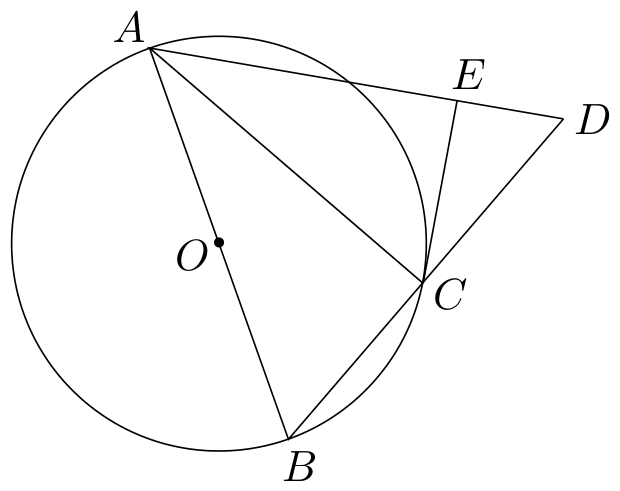
\includegraphics[width=7.7cm]{GaoKao/images/2013/guangdong_science/q15_fig1.png}
\end{center}

    \end{enumerate}

\end{description}

\begin{description}

    \item[四、解答题]

    \begin{enumerate}[leftmargin=5pt]

      \addtocounter{enumi}{+15}

        \item 已知函数 \(f(x) = \sqrt{2}\cos\left(x - \frac{\pi}{12}\right)\)，\(x \in \mathbb{R}\).

\begin{enumerate}
\item 求 \(f\left(-\frac{\pi}{6}\right)\) 的值.
\item 若 \(\cos \theta = \frac{3}{5}\)，\(\theta \in \left(\frac{3\pi}{2}, 2\pi\right)\)，求 \(f\left(2\theta + \frac{\pi}{3}\right)\).
\end{enumerate}

        \item 某车间共有 \(12\) 名工人，随机抽取 \(6\) 名，他们某日加工零件个数的茎叶图如图所示，其中茎为十位数，叶为个位数.

\begin{center}
\begin{tabular}{c|l}
1 & \(7\;9\) \\
2 & \(0\;1\;5\) \\
3 & \(0\)
\end{tabular}
\end{center}

\begin{enumerate}
\item 根据茎叶图计算样本均值.
\item 日加工零件个数大于样本均值的工人为优秀工人. 根据茎叶图推断该车间 \(12\) 名工人中有几名优秀工人？
\item 从该车间 \(12\) 名工人中，任取 \(2\) 人，求恰有 \(1\) 名优秀工人的概率.
\end{enumerate}

        \item 如图\ding{172}，在等腰直角三角形 \(ABC\) 中，\(\angle A = 90^{\circ}\)，\(BC = 6\).
\(D\)，\(E\) 分别是 \(AC\)，\(AB\) 上的点，\(CD = BE = \sqrt{2}\)，\(O\) 为 \(BC\) 的中点.
将 \(\triangle ADE\) 沿 \(DE\) 折起，得到下图\ding{173}所示的四棱锥 \(A^{\prime} - BCDE\)，其中 \(A^{\prime}O = \sqrt{3}\).

\begin{enumerate}
\item 证明：\(A^{\prime}O \perp\) 平面 \(BCDE\).
\item 求二面角 \(A^{\prime} - CD - B\) 的平面角的余弦值.
\end{enumerate}

\begin{center}
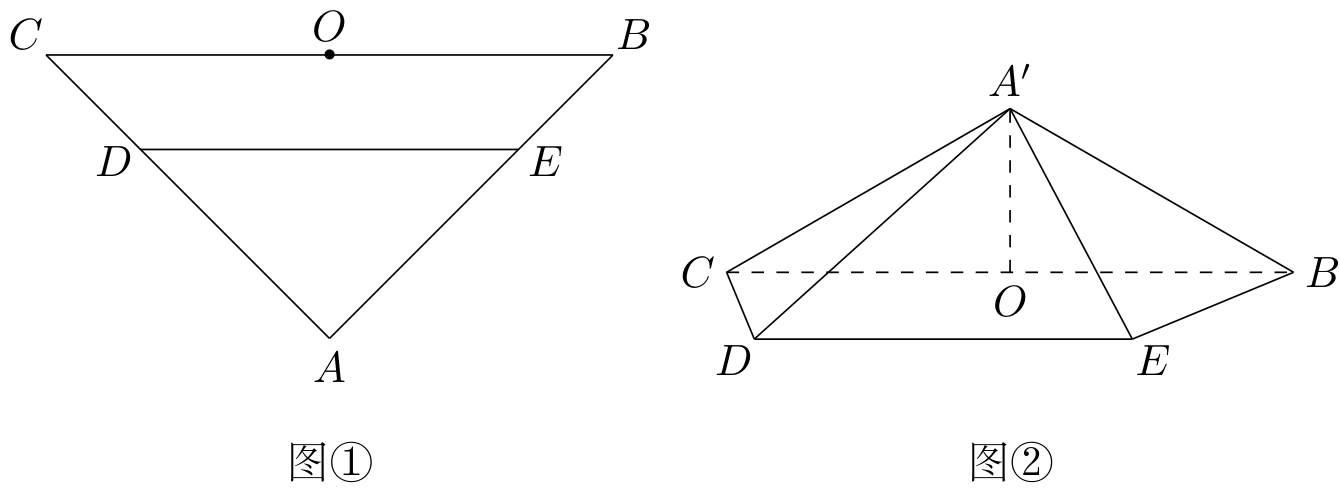
\includegraphics[width=13.0cm]{GaoKao/images/2013/guangdong_science/q18_fig1.png}
\end{center}

        \item 设数列 \(\{a_{n}\}\) 的前 \(n\) 项和为 \(S_{n}\)，已知 \(a_{1} = 1\)，\(\frac{2S_{n}}{n} = a_{n+1} - \frac{1}{3} n^{2} - n - \frac{2}{3}\)，\(n \in \mathbf{N}^{*}\).

\begin{enumerate}
\item 求 \(a_{2}\) 的值.
\item 求数列 \(\{a_{n}\}\) 的通项公式.
\item 证明：对一切正整数 \(n\)，有 \(\frac{1}{a_1} + \frac{1}{a_2} + \cdots + \frac{1}{a_n} < \frac{7}{4}\).
\end{enumerate}

        \item 已知抛物线 \(C\) 的顶点为原点，其焦点 \(F(0, c)\)（\(c > 0\)）到直线 \(l: x - y - 2 = 0\) 的距离为 \(\frac{3\sqrt{2}}{2}\). 设 \(P\) 为直线 \(l\) 上的点，过点 \(P\) 作抛物线 \(C\) 的两条切线 \(PA\)，\(PB\)，其中 \(A\)，\(B\) 为切点.

\begin{enumerate}
\item 求抛物线 \(C\) 的方程.
\item 当点 \(P(x_0, y_0)\) 为直线 \(l\) 上的定点时，求直线 \(AB\) 的方程.
\item 当点 \(P\) 在直线 \(l\) 上移动时，求 \(|AF| \cdot |BF|\) 的最小值.
\end{enumerate}

        \item 设函数 \(f(x) = (x - 1){\mathrm{e}}^{x} - kx^{2} \) （\(k \in \mathbb{R}\)）.

\begin{enumerate}
\item 当 \(k = 1\) 时，求函数 \(f(x)\) 的单调区间.
\item 当 \(k \in \left(\frac{1}{2}, 1\right]\) 时，求函数 \(f(x)\) 在 \([0, k]\) 上的最大值 \(M\).
\end{enumerate}

    \end{enumerate}

\end{description}


\subsection{2013年广东卷（文）}\label{gk:2013年广东卷（文）}

\begin{description}

    \item[一、选择题]

    \begin{enumerate}[leftmargin=5pt]

        \item 设集合 \(S = \{x \mid x^2 + 2x = 0, x \in \mathbb{R}\}\)，\(T = \{x \mid x^2 - 2x = 0, x \in \mathbb{R}\}\)，则 \(S \cap T =\)（\quad）

        {\centering\begin{tabular*}{\linewidth}{@{}@{\extracolsep{\fill}}llll@{}}
          \text{A. }\( \{0\} \)  &  \text{B. }\(\{0, 2\}\)  &  \text{C. }\(\{-2, 0\}\)  &  \text{D. }\(\{-2, 0, 2\}\)
        \end{tabular*}\par}

        \item 函数 \( y = \frac{\lg(x + 1)}{x - 1} \) 的定义域是（\quad）

        {\centering\begin{tabular*}{\linewidth}{@{}@{\extracolsep{\fill}}llll@{}}
          \text{A. }\( (-1,+\infty) \)  &  \text{B. }\( [-1,+\infty) \)  &  \text{C. }\( (-1,1)\cup(1,+\infty) \)  &  \text{D. }\([-1, 1) \cup (1, +\infty)\)
        \end{tabular*}\par}

        \item 若 \(\i (x + y\i) = 3 + 4\i\)，\(x\)，\(y \in \mathbb{R}\)，则复数 \( x + y\i \) 的模是（\quad）

        {\centering\begin{tabular*}{\linewidth}{@{}@{\extracolsep{\fill}}llll@{}}
          \text{A. }\(2\)  &  \text{B. }\(3\)  &  \text{C. }\(4\)  &  \text{D. }\(5\)
        \end{tabular*}\par}

        \item 已知 \(\sin \left(\frac{5\pi}{2} + \alpha\right) = \frac{1}{5}\)，那么 \(\cos \alpha =\)（\quad）

        {\centering\begin{tabular*}{\linewidth}{@{}@{\extracolsep{\fill}}llll@{}}
          \text{A. }\(-\frac{2}{5}\)  &  \text{B. }\(-\frac{1}{5}\)  &  \text{C. }\(\frac{1}{5}\)  &  \text{D. }\(\frac{2}{5}\)
        \end{tabular*}\par}

        \item 执行如图所示的程序框图，若输入 \(n\) 的值为 3 ，则输出 \(s\) 的值是（\quad）

\begin{center}
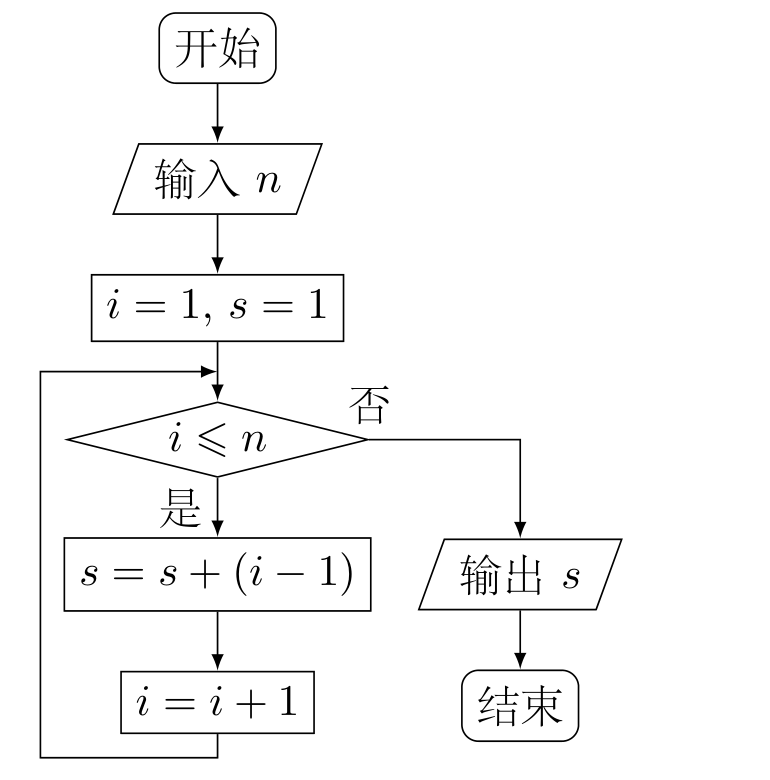
\includegraphics[width=0.34\linewidth]{GaoKao/images/2013/guangdong_liberal/q5_fig1.png}
\end{center}

        {\centering\begin{tabular*}{\linewidth}{@{}@{\extracolsep{\fill}}llll@{}}
          \text{A. }\(1\)  &  \text{B. }\(2\)  &  \text{C. }\(4\)  &  \text{D. }\(7\)
        \end{tabular*}\par}

        \item 某三棱锥的三视图如图所示，则该三棱锥的体积是（\quad）

\begin{center}
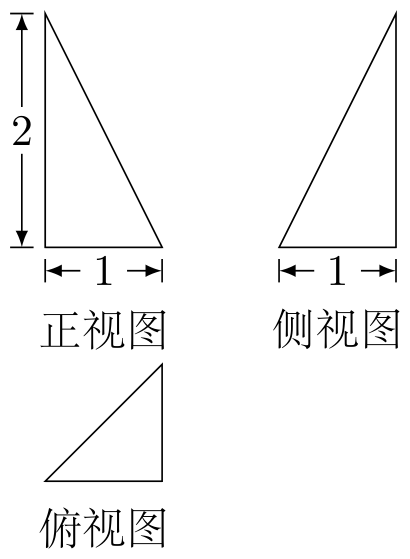
\includegraphics[width=4.0cm]{GaoKao/images/2013/guangdong_liberal/q6_fig1.png}
\end{center}

        {\centering\begin{tabular*}{\linewidth}{@{}@{\extracolsep{\fill}}llll@{}}
          \text{A. }\( \frac{1}{6} \)  &  \text{B. }\( \frac{1}{3} \)  &  \text{C. }\( \frac{2}{3} \)  &  \text{D. }\(1\)
        \end{tabular*}\par}

        \item 垂直于直线 \( y = x + 1 \) 且与圆 \( x^{2} + y^{2} = 1 \) 相切于第一象限的直线方程是（\quad）

        {\centering\begin{tabular*}{\linewidth}{@{}@{\extracolsep{\fill}}llll@{}}
          \text{A. }\(x + y - \sqrt{2} = 0\)  &  \text{B. }\(x + y + 1 = 0\)  &  \text{C. }\(x + y - 1 = 0\)  &  \text{D. }\(x + y + \sqrt{2} = 0\)
        \end{tabular*}\par}

        \item 设 \(l\) 为直线，\(\alpha\)，\(\beta\) 是两个不同的平面，下列命题中正确的是（\quad）

        {\centering\begin{tabular*}{\linewidth}{@{}@{\extracolsep{\fill}}llll@{}}
          \text{A. }若 \(l \parallel \alpha, l \parallel \beta\)，则 \(\alpha \parallel \beta\)  &  \text{B. }若 \(l \perp \alpha\)，\(l \perp \beta\)，则 \(\alpha \parallel \beta\)  &  \text{C. }若 \(l \perp \alpha\)，\(l \parallel \beta\)，则 \(\alpha \parallel \beta\)  &  \text{D. }若 \(\alpha \perp \beta\)，\(l \parallel \alpha\)，则 \(l \perp \beta\)
        \end{tabular*}\par}

        \item 已知中心在原点的椭圆 \(C\) 的右焦点为 \(F(1,0)\). 离心率等于 \(\frac{1}{2}\)，则 \(C\) 的方程是（\quad）

        {\centering\begin{tabular*}{\linewidth}{@{}@{\extracolsep{\fill}}llll@{}}
          \text{A. }\(\frac{x^2}{3} +\frac{y^2}{4} = 1\)  &  \text{B. }\(\frac{x^2}{4} +\frac{y^2}{\sqrt{3}} = 1\)  &  \text{C. }\(\frac{x^2}{4} +\frac{y^2}{2} = 1\)  &  \text{D. }\(\frac{x^2}{4} +\frac{y^2}{3} = 1\)
        \end{tabular*}\par}

        \item 设 \(\bm{a}\) 是已知的平面向量且 \(\bm{a} \neq 0\). 关于向量 \(\bm{a}\) 的分解，有如下四个命题：
\begin{enumerate}
\item 给定向量 \(\bm{b}\)，总存在向量 \(\bm{c}\)，使 \(\bm{a} = \bm{b} + \bm{c}\).
\item 给定向量 \(\bm{b}\) 和 \(\bm{c}\)，总存在实数 \(\lambda\) 和 \(\mu\)，使 \(\bm{a} = \lambda \bm{b} + \mu \bm{c}\)；
\item 给定单位向量 \(\bm{b}\) 和正数 \(\mu\)，总存在单位向量 \(\bm{c}\) 和实数 \(\lambda\)，使 \(\bm{a} = \lambda \bm{b} + \mu \bm{c}\).
\item 给定正数 \(\lambda\) 和 \(\mu\)，总存在单位向量 \(\bm{b}\) 和单位向量 \(\bm{c}\)，使 \(\bm{a} = \lambda \bm{b} + \mu \bm{c}\).
\end{enumerate}

上述命题中的向量 \(\bm{b}\)，\(\bm{c}\) 和 \(\bm{a}\) 在同一平面内且两两不共线，
则真命题的个数是（\quad）

        {\centering\begin{tabular*}{\linewidth}{@{}@{\extracolsep{\fill}}llll@{}}
          \text{A. }\(1\)  &  \text{B. }\(2\)  &  \text{C. }\(3\)  &  \text{D. }\(4\)
        \end{tabular*}\par}

    \end{enumerate}

\end{description}

\begin{description}

    \item[二、填空题]

    \begin{enumerate}[leftmargin=5pt]

      \addtocounter{enumi}{+10}

        \item 设数列 \( \{a_{n}\} \) 是首项为 1，公比为 \(-2\) 的等比数列，则 \( a_{1} + |a_{2}| + a_{3} + |a_{4}| = \)\rule[-0.3ex]{3em}{0.4pt}.

        \item 若曲线 \( y = ax^2 - \ln x \) 在点 \((1, a)\) 处的切线平行于 \( x \) 轴，则 \( a = \)\rule[-0.3ex]{3em}{0.4pt}.

        \item 已知变量 \(x\)，\(y\) 满足约束条件 \(\begin{cases}
x - y + 3 \geqslant 0,\\
-1 \leqslant x \leqslant 1,\\
y \geqslant 1,
\end{cases}\) 则 \(z = x + y\) 的最大值是\rule[-0.3ex]{3em}{0.4pt}.

    \end{enumerate}

\end{description}

\begin{description}

    \item[三、选考题]

    \begin{enumerate}[leftmargin=5pt]

      \addtocounter{enumi}{+13}

        \item \textbf{【选修4-4：坐标系与参数方程】}

已知曲线 \(C\) 的极坐标方程为 \(\rho = 2\cos \theta\)，以极点为原点，极轴为 \(x\) 轴的正半轴建立直角坐标系，则曲线 \(C\) 的参数方程为\rule[-0.3ex]{3em}{0.4pt}.

        \item 如图，在矩形 \(ABCD\) 中，\(AB = \sqrt{3}\)，\(BC = 3\)，\(BE \perp AC\)，垂足为 \(E\)，则 \(ED = \)\rule[-0.3ex]{3em}{0.4pt}.

\begin{center}
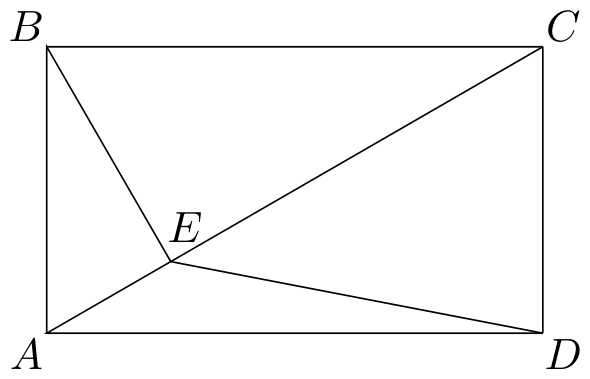
\includegraphics[width=7.1cm]{GaoKao/images/2013/guangdong_liberal/q15_fig1.png}
\end{center}

    \end{enumerate}

\end{description}

\begin{description}

    \item[四、解答题]

    \begin{enumerate}[leftmargin=5pt]

      \addtocounter{enumi}{+15}

        \item 已知函数 \(f(x) = \sqrt{2}\cos \left(x - \frac{\pi}{12}\right)\)，\(x \in \mathbb{R}\).
\begin{enumerate}
\item 求 \( f\left(\frac{\pi}{3}\right) \) 的值；
\item 若 \(\cos\theta=\frac{3}{5}\)，\(\theta\in\left(\frac{3\pi}{2},2\pi\right)\)，求 \( f\left(\theta-\frac{\pi}{6}\right) \).
\end{enumerate}

        \item 从一批苹果中，随机抽取 \(50\) 个，其重量（单位：克）的频数分布表如下：

\begin{center}
\begin{tabular}{c|cccc}
分组（重量） & \( [80,85) \) & \( [85,90) \) & \( [90,95) \) & \( [95,100) \) \\
\hline
频数 & \(5\) & \(10\) & \(20\) & \(15\)
\end{tabular}
\end{center}

\begin{enumerate}
\item 根据频数分布表计算苹果的重量在 \([90,95)\) 的频率；
\item 用分层抽样的方法从重量在 \([80,85)\) 和 \([95,100)\) 的苹果中共抽取 4 个，其中重量在 \([80,85)\) 的有几个？
\item 在（2）中抽出的 4 个苹果中，任取 2 个，求重量在 \([80,85)\) 和 \([95,100)\) 中各有 1 个的概率.
\end{enumerate}

        \item 如图\ding{172}，在边长为 1 的等边三角形 \(ABC\) 中，\(D\)，\(E\) 分别是 \(AB\)，\(AC\) 上的点，\(AD = AE\)，\(F\) 是 \(BC\) 的中点，\(AF\) 与 \(DE\) 交于点 \(G\)，将 \(\triangle ABF\) 沿 \(AF\) 折起，得到如图\ding{173}所示的三棱锥 \(A - BCF\)，其中 \(BC = \frac{\sqrt{2}}{2}\).
\begin{enumerate}
\item 证明： \(DE \parallel\) 平面 \(BCF\)；
\item 证明： \(CF \perp\) 平面 \(ABF\)；
\item 当 \(AD = \frac{2}{3}\) 时，求三棱锥 \(F - DEG\) 的体积 \(V_{F - DEG}\).
\end{enumerate}

\begin{center}
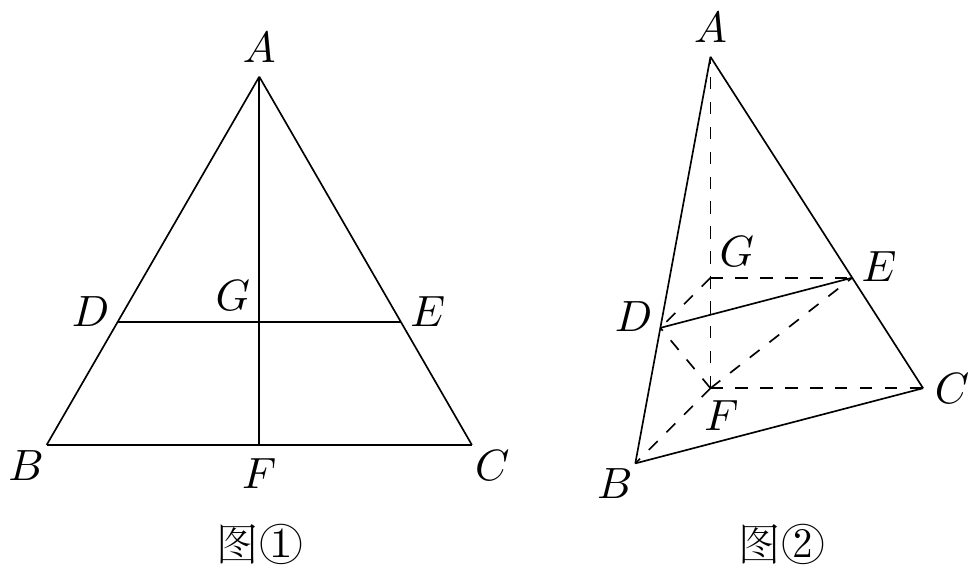
\includegraphics[width=9.5cm]{GaoKao/images/2013/guangdong_liberal/q18_fig1.png}
\end{center}

        \item 设各项均为正数的数列 \(\{a_{n}\}\) 的前 \(n\) 项和为 \(S_{n}\)，满足 \(4S_{n} = a_{n+1}^{2} - 4n - 1\)，\(n \in \mathbf{N}^{*}\)，且 \(a_{2}\)，\(a_{5}\)，\(a_{14}\) 构成等比数列.
\begin{enumerate}
\item 证明： \(a_{2} = \sqrt{4a_{1} + 5}\)；
\item 求数列 \(\{a_n\}\) 的通项公式；
\item 证明：对一切正整数 \(n\)，有 \(\frac{1}{a_1 a_2} + \frac{1}{a_2 a_3} + \cdots + \frac{1}{a_n a_{n+1}} < \frac{1}{2}\).
\end{enumerate}

        \item 已知抛物线 \(C\) 的顶点为原点，其焦点 \(F(0, c)\)（\(c > 0\)）到直线 \(l\)：\(x - y - 2 = 0\) 的距离为 \(\frac{3\sqrt{2}}{2}\). 设 \(P\) 为直线 \(l\) 上的点，过点 \(P\) 作抛物线 \(C\) 的两条切线 \(PA\)，\(PB\)，其中 \(A\)，\(B\) 为切点.
\begin{enumerate}
\item 求抛物线 \(C\) 的方程；
\item 当点 \(P(x_0, y_0)\) 为直线 \(l\) 上的定点时，求直线 \(AB\) 的方程；
\item 当点 \(P\) 在直线 \(l\) 上移动时，求 \(|AF| \cdot |BF|\) 的最小值.
\end{enumerate}

        \item 设函数 \( f(x) = x^3 - kx^2 + x  \)（\(x \in \mathbb{R}\)）.
\begin{enumerate}
\item 当 \(k = 1\) 时，求函数 \(f(x)\) 的单调区间；
\item 当 \(k < 0\) 时，求函数 \(f(x)\) 在 \([k, -k]\) 上的最小值 \(m\) 和最大值 \(M\).
\end{enumerate}

    \end{enumerate}

\end{description}


\subsection{2013年湖北卷（理）}\label{gk:2013年湖北卷（理）}

\begin{description}

    \item[一、选择题]

    \begin{enumerate}[leftmargin=5pt]

        \item 在复平面内，复数 \(z = \frac{2\i}{1 + \i}\)（\(\i\) 为虚数单位）的共轭复数对应的点位于（\quad）

        {\centering\begin{tabular*}{\linewidth}{@{}@{\extracolsep{\fill}}llll@{}}
          \text{A. }第一象限  &  \text{B. }第二象限  &  \text{C. }第三象限  &  \text{D. }第四象限
        \end{tabular*}\par}

        \item 已知全集为 \(\mathbb{R}\). 集合 \(A = \left\{x \mid \left(\frac{1}{2}\right)^x \leqslant 1\right\}\)，\(B = \{x \mid x^2 - 6x + 8 \leqslant 0\}\)，则 \(A \cap \complement_{\mathbb{R}} B =\)（\quad）

        {\centering\begin{tabular*}{\linewidth}{@{}@{\extracolsep{\fill}}llll@{}}
          \text{A. }\(\{x \mid x \leqslant 0\}\)  &  \text{B. }\(\{x \mid 2 \leqslant x \leqslant 4\}\)  &  \text{C. }\(\{x \mid 0 \leqslant x < 2\}\) 或 \(\{x \mid x > 4\}\)  &  \text{D. }\(\{x \mid 0 < x \leqslant 2\}\) 或 \(\{x \mid x \geqslant 4\}\)
        \end{tabular*}\par}

        \item 在一次跳伞训练中，甲，乙两位学员各跳一次. 设命题 \(p\) 是“甲降落在指定范围”，\(q\) 是“乙降落在指定范围”，则命题“至少有一位学员没有降落在指定范围”可表示为（\quad）

        {\centering\begin{tabular*}{\linewidth}{@{}@{\extracolsep{\fill}}llll@{}}
          \text{A. }\((\neg p) \vee (\neg q)\)  &  \text{B. }\(p \vee (\neg q)\)  &  \text{C. }\((\neg p) \wedge (\neg q)\)  &  \text{D. }\(p \vee q\)
        \end{tabular*}\par}

        \item 将函数 \( y = \sqrt{3} \cos x + \sin x \)（\(x \in \mathbb{R}\)）的图像向左平移 \(m\)（\(m > 0\)）个单位长度后，所得到的图象关于 \(y\) 轴对称. 则 \(m\) 的最小值是（\quad）

        {\centering\begin{tabular*}{\linewidth}{@{}@{\extracolsep{\fill}}llll@{}}
          \text{A. }\(\frac{\pi}{12}\)  &  \text{B. }\(\frac{\pi}{6}\)  &  \text{C. }\(\frac{\pi}{3}\)  &  \text{D. }\(\frac{5\pi}{6}\)
        \end{tabular*}\par}

        \item 已知 \(0 < \theta < \frac{\pi}{4}\)，则双曲线 \(C_1: \frac{x^{2}}{\cos^{2}\theta} - \frac{y^{2}}{\sin^{2}\theta} = 1\) 与 \(C_2: \frac{y^{2}}{\sin^{2}\theta} - \frac{x^{2}}{\sin^{2}\theta \tan^{2}\theta} = 1\) 的（\quad）

        {\centering\begin{tabular*}{\linewidth}{@{}@{\extracolsep{\fill}}llll@{}}
          \text{A. }实轴长相等  &  \text{B. }虚轴长相等  &  \text{C. }焦距相等  &  \text{D. }离心率相等
        \end{tabular*}\par}

        \item 已知点 \(A(-1,1)\)，\(B(1,2)\)，\(C(-2,-1)\)，\(D(3,4)\). 则向量 \(\overrightarrow{AB}\) 在 \(\overrightarrow{CD}\) 方向上的投影为（\quad）

        {\centering\begin{tabular*}{\linewidth}{@{}@{\extracolsep{\fill}}llll@{}}
          \text{A. }\(\frac{3\sqrt{2}}{2}\)  &  \text{B. }\(\frac{3\sqrt{15}}{2}\)  &  \text{C. }\(-\frac{3\sqrt{2}}{2}\)  &  \text{D. }\(-\frac{3\sqrt{15}}{2}\)
        \end{tabular*}\par}

        \item 一辆汽车在高速公路上行驶，由于遇到紧急情况而刹车，以速度 \(v(t) = 7 - 3t + \frac{25}{1 + t}\)（\(t\) 的单位：\(\mathrm{s}\)，\(v\) 的单位：\(\mathrm{m/s}\)）行驶至停止，在此期间汽车继续行驶的距离（单位：\(\mathrm{m}\)）是（\quad）

        {\centering\begin{tabular*}{\linewidth}{@{}@{\extracolsep{\fill}}llll@{}}
          \text{A. }\(1 + 25\ln 5\)  &  \text{B. }\(8 + 25\ln \frac{11}{3}\)  &  \text{C. }\(4 + 25\ln 5\)  &  \text{D. }\(4 + 50\ln 2\)
        \end{tabular*}\par}

        \item 一个几何体的三视图如图所示，该几何体从上到下由四个简单几何体组成，其体积分别记为 \(V_{1}\)，\(V_{2}\)，\(V_{3}\)，\(V_{4}\). 上面两个简单几何体均为旋转体，下面两个简单几何体均为多面体，则有（\quad）

\begin{center}
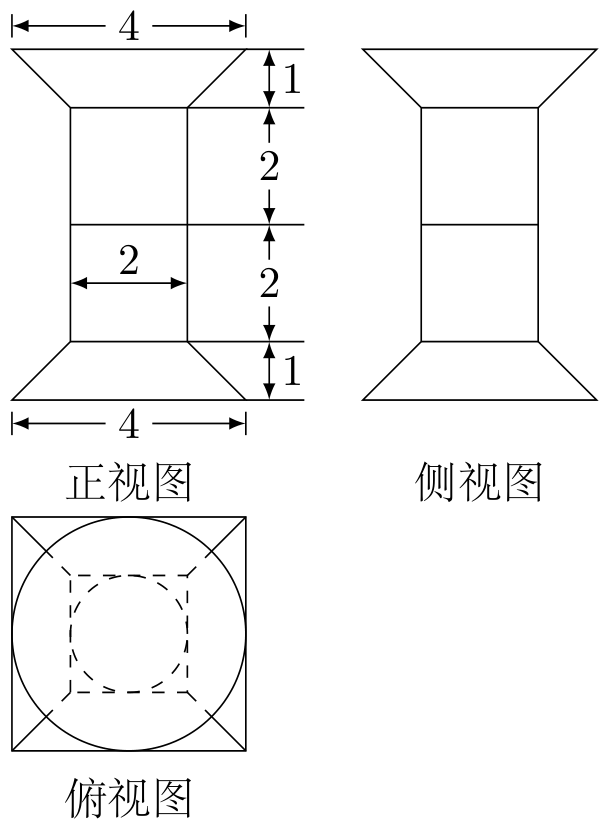
\includegraphics[width=5.9cm]{GaoKao/images/2013/hubei_science/q8_fig1.png}
\end{center}

        {\centering\begin{tabular*}{\linewidth}{@{}@{\extracolsep{\fill}}llll@{}}
          \text{A. }\(V_{1} < V_{2} < V_{4} < V_{3}\)  &  \text{B. }\(V_{1} < V_{3} < V_{2} < V_{4}\)  &  \text{C. }\(V_{2} < V_{1} < V_{3} < V_{4}\)  &  \text{D. }\(V_{2} < V_{3} < V_{1} < V_{4}\)
        \end{tabular*}\par}

        \item 如图，将一个各面都涂了油漆的正方体切割为 125 个同样大小的小正方体，经过搅拌后，从中随机取一个小正方体，记其涂漆面数为 \(X\)，则 \(X\) 的均值 \(E(X) =\)（\quad）

\begin{center}
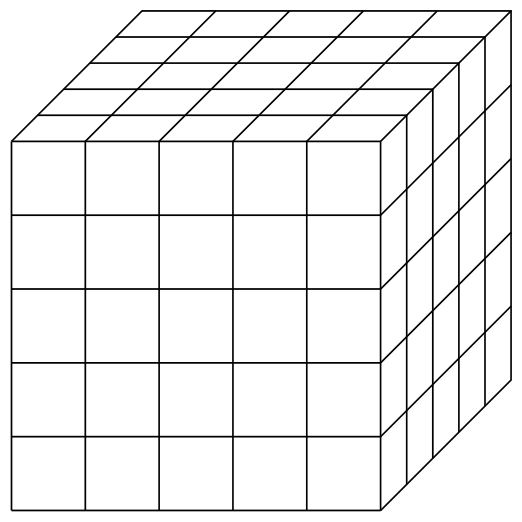
\includegraphics[width=8.8cm]{GaoKao/images/2013/hubei_science/q9_fig1.png}
\end{center}

        {\centering\begin{tabular*}{\linewidth}{@{}@{\extracolsep{\fill}}llll@{}}
          \text{A. }\(\frac{126}{125}\)  &  \text{B. }\(\frac{6}{5}\)  &  \text{C. }\(\frac{168}{125}\)  &  \text{D. }\(\frac{7}{5}\)
        \end{tabular*}\par}

        \item 已知 \(a\) 为常数，函数 \(f(x) = x(\ln x - ax)\) 有两个极值点 \(x_1\)，\(x_2\)（\(x_1 < x_2\)），则（\quad）

        {\centering\begin{tabular*}{\linewidth}{@{}@{\extracolsep{\fill}}llll@{}}
          \text{A. }\(f(x_1) > 0\)，\(f(x_2) > -\frac{1}{2}\)  &  \text{B. }\(f(x_1) < 0\)，\(f(x_2) < -\frac{1}{2}\)  &  \text{C. }\(f(x_1) > 0\)，\(f(x_2) < -\frac{1}{2}\)  &  \text{D. }\(f(x_1) < 0\)，\(f(x_2) > -\frac{1}{2}\)
        \end{tabular*}\par}

    \end{enumerate}

\end{description}

\begin{description}

    \item[二、填空题]

    \begin{enumerate}[leftmargin=5pt]

      \addtocounter{enumi}{+10}

        \item 从某小区抽取 100 户居民进行月用电量调查，发现其用电量都在 50 至 350 度之间，频率分布直方图如图所示.

\begin{enumerate}
\item 直方图中 \(x\) 的值为\rule[-0.3ex]{3em}{0.4pt}；
\item 在这些用户中，用电量落在区间 \([100,250)\) 内的户数为\rule[-0.3ex]{3em}{0.4pt}.
\end{enumerate}

\begin{center}
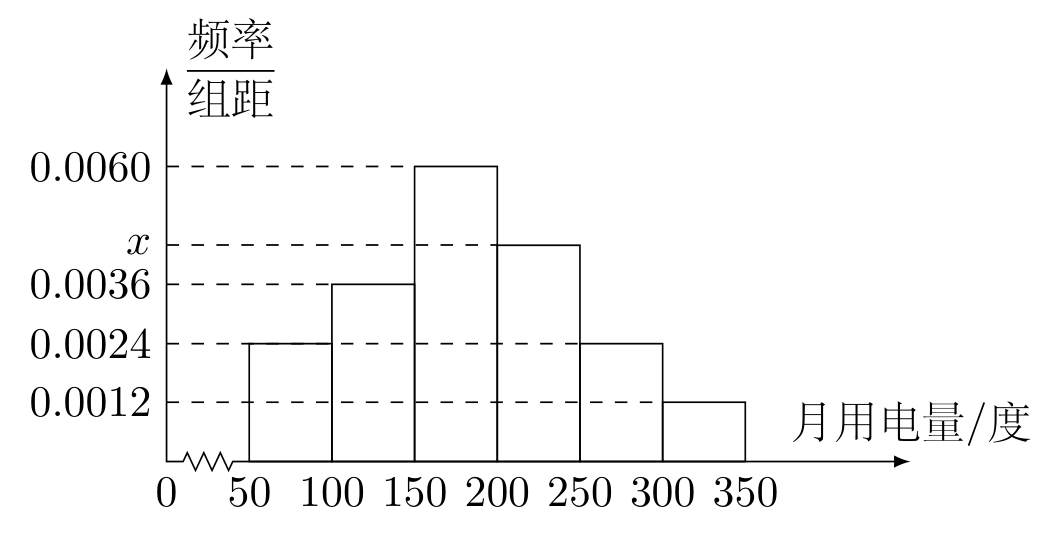
\includegraphics[width=0.45\linewidth]{GaoKao/images/2013/hubei_science/q11_fig1.png}
\end{center}

        \item 阅读如图所示的程序框图，运行相应的程序，输出的结果 \(i=\rule[-0.3ex]{3em}{0.4pt}\).

\begin{center}
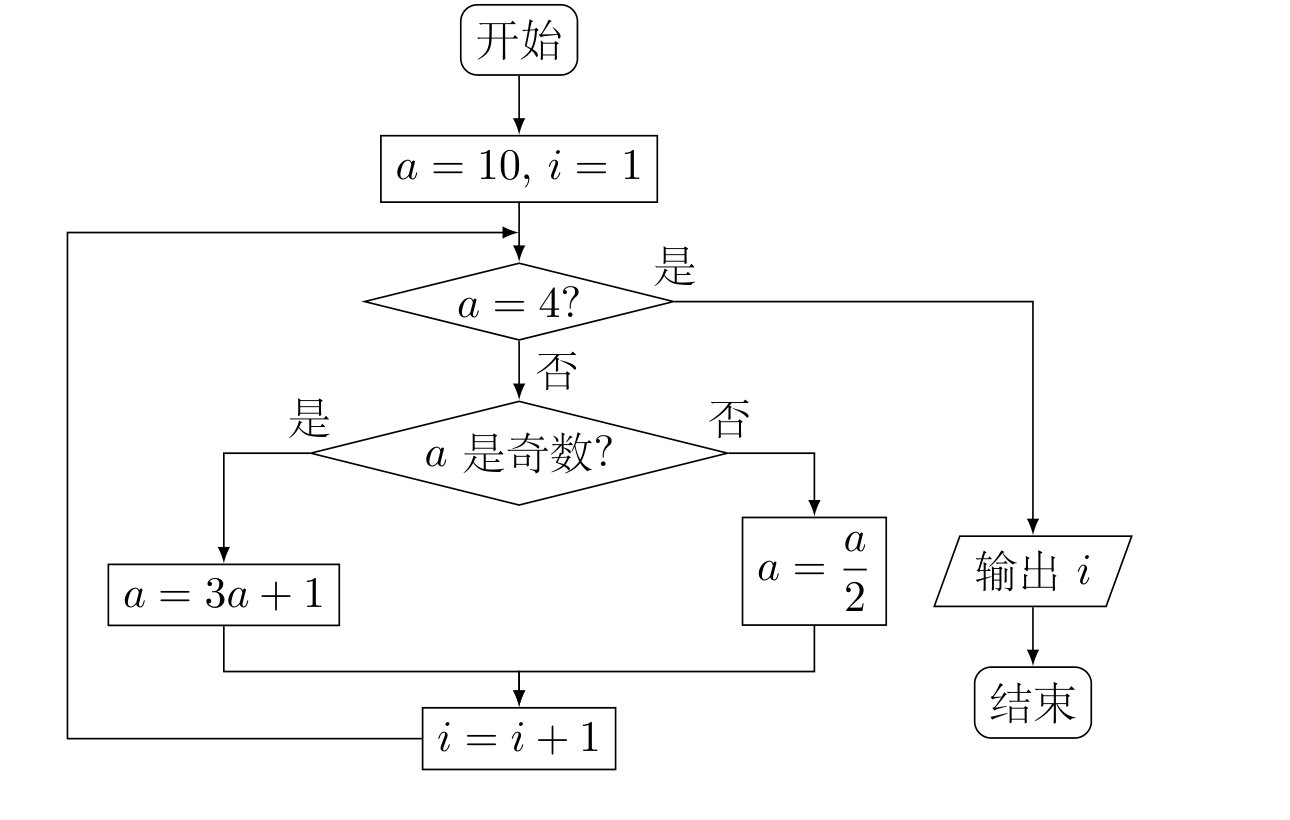
\includegraphics[width=0.46\linewidth]{GaoKao/images/2013/hubei_science/q12_fig1.png}
\end{center}

        \item 设 \(x\)，\(y\)，\(z \in \mathbb{R}\)，且满足：\(x^2 + y^2 + z^2 = 1\)，\(x + 2y + 3z = \sqrt{14}\)，则 \(x + y + z =\rule[-0.3ex]{3em}{0.4pt}\).

        \item 古希腊毕达哥拉斯学派的数学家研究过各种多边形数，如三角形数 \(1\)，\(3\)，\(6\)，\(10\)，\(\cdots\)，第 \(n\) 个三角形数为 \(\frac{n(n + 1)}{2} = \frac{1}{2}n^2 + \frac{1}{2}n\). 记第 \(n\) 个 \(k\) 边形数为 \(N(n, k)\)（\(k \geqslant 3\)），以下列出了部分 \(k\) 边形数中第 \(n\) 个数的表达式：

三角形数 \(N(n, 3) = \frac{1}{2}n^2 + \frac{1}{2}n\)，
正方形数 \(N(n, 4) = n^2\)，
五边形数 \(N(n, 5) = \frac{3}{2}n^2 - \frac{1}{2}n\)，
六边形数 \(N(n, 6) = 2n^2 - n\)，
……

可以推测 \(N(n, k)\) 的表达式，由此计算 \(N(10, 24) =\rule[-0.3ex]{3em}{0.4pt}.\)

    \end{enumerate}

\end{description}

\begin{description}

    \item[三、选考题]

    \begin{enumerate}[leftmargin=5pt]

      \addtocounter{enumi}{+14}

        \item \textbf{【选修4-1：几何证明选讲】}

如图，圆 \(O\) 上一点 \(C\) 在直径 \(AB\) 上的射影为 \(D\)，点 \(D\) 在半径 \(OC\) 上的射影为 \(E\)，若 \(AB = 3AD\)，则 \(\dfrac{CE}{EO}\) 的值为\rule[-0.3ex]{3em}{0.4pt}.

\begin{center}
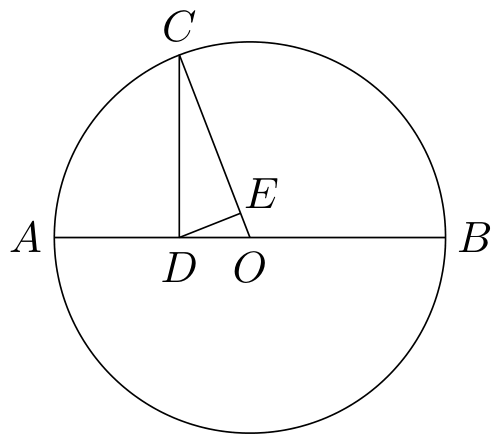
\includegraphics[width=5.8cm]{GaoKao/images/2013/hubei_science/q15_fig1.png}
\end{center}

        \item \textbf{【选修4-4：坐标系与参数方程】}

在直角坐标系 \(xOy\) 中，椭圆 \(C\) 的参数方程为 \(\begin{cases}
x = a\cos\varphi,\\
y = b\sin\varphi,
\end{cases}\)
（\(\varphi\) 为参数，\(a > b > 0\)），在极坐标系（与直角坐标系 \(xOy\) 取相同的长度单位，且以原点 \(O\) 为极点，以 \(x\) 轴正半轴为极轴）中，直线 \(l\) 与圆 \(O\) 的极坐标方程分别为 \(\rho\sin\left(\theta + \frac{\pi}{4}\right) = \frac{\sqrt{2}}{2}m\)（\(m\) 为非零常数）与 \(\rho = b\)，若直线 \(l\) 经过椭圆 \(C\) 的焦点，且与圆 \(O\) 相切，则椭圆 \(C\) 的离心率为\rule[-0.3ex]{3em}{0.4pt}.

    \end{enumerate}

\end{description}

\begin{description}

    \item[四、解答题]

    \begin{enumerate}[leftmargin=5pt]

      \addtocounter{enumi}{+16}

        \item 在 \(\triangle ABC\) 中，角 \(A\)，\(B\)，\(C\) 对应的边分别是 \(a\)，\(b\)，\(c\). 已知 \(\cos 2A - 3\cos (B + C) = 1\).
\begin{enumerate}
\item 求角 \(A\) 的大小；
\item 若 \(\triangle ABC\) 的面积 \(S = 5\sqrt{3}\)，\(b = 5\)，求 \(\sin B \sin C\) 的值.
\end{enumerate}

        \item 已知等比数列 \(\{a_{n}\}\) 满足：\(\left|a_2 - a_3\right| = 10\)，\(a_1a_2a_3 = 125\).
\begin{enumerate}
\item 求数列 \(\{a_{n}\}\) 的通项公式；
\item 是否存在正整数 \(m\)，使得 \(\frac{1}{a_1} + \frac{1}{a_2} + \cdots + \frac{1}{a_m} \geqslant 1\). 若存在，求 \(m\) 的最小值；若不存在，说明理由.
\end{enumerate}

        \item 如图，\(AB\) 是圆 \(O\) 的直径，点 \(C\) 是圆 \(O\) 上异于 \(A\)，\(B\) 的点，直线 \(PC \perp\) 平面 \(ABC\)，\(E\)，\(F\) 分别是 \(PA\)，\(PC\) 的中点.
\begin{enumerate}
\item 记平面 \(BEF\) 与平面 \(ABC\) 的交线为 \(l\)，试判断直线 \(l\) 与平面 PAC 的位置关系，并加以证明；
\item 设 （1） 中的直线 \(l\) 与圆 \(O\) 的另一个交点为 \(D\)，且点 \(Q\) 满足 \(\overrightarrow{DQ} = \frac{1}{2}\overrightarrow{CP}\)，记直线 \(PQ\) 与平面 \(ABC\) 所成的角为 \(\theta\)，异面直线 \(PQ\) 与 \(EF\) 所成的角为 \(\alpha\)，二面角 \(E - l - C\) 的大小为 \(\beta\)，求证： \(\sin \theta = \sin \alpha \sin \beta\).
\end{enumerate}

        \item 假设每天从甲地去乙地的旅客人数 \(X\) 是服从正态分布 \(N(800,50^{2})\) 的随机变量，记一天中从甲地去乙地的旅客人数不超过 900 的概率为 \(P_{0}\).
\begin{enumerate}
\item 求 \(P_{0}\) 的值；（参考数据：若 \(X \sim N(\mu, \sigma^{2})\)，有 \(P(\mu - \sigma < X \leqslant \mu + \sigma) = 0.6826\)，\(P(\mu - 2\sigma < X \leqslant \mu + 2\sigma) = 0.9544\)，\(P(\mu - 3\sigma < X \leqslant \mu + 3\sigma) = 0.9974\)）
\item 某客运公司用 \(A\)，\(B\) 两种型号的车辆承担甲，乙两地间的长途客运业务，每车每天往返一次，\(A\)，\(B\) 两种车辆的载客量分别为 36 人和 60 人，从甲地去乙地的营运成本分别为 1600 元/辆和 2400 元/辆. 公司拟组建一个不超过 21 辆车的客运车队，并要求 \(B\) 型车不多于 \(A\) 型车 7 辆. 若每天要以不小于 \(p_0\) 的概率运完从甲地去乙地的旅客，且使公司从甲地去乙地的营运成本最小，那么应配备 \(A\) 型车，\(B\) 型车各多少辆？
\end{enumerate}

        \item 如图，已知椭圆 \(C_1\) 与 \(C_2\) 的中心在坐标原点 \(O\)，长轴均为 \(MN\) 且在 \(x\) 轴上，短轴长分别为 \(2m\)，\(2n\)（\(m > n\)），过原点且不与 \(x\) 轴重合的直线 \(l\) 与 \(C_1\)，\(C_2\) 的四个交点按纵坐标从大到小依次为 \(A\)，\(B\)，\(C\)，\(D\)，记 \(\lambda = \frac{m}{n}\)，\(\triangle BDM\) 和 \(\triangle ABN\) 的面积分别为 \(S_1\) 和 \(S_2\).
\begin{enumerate}
\item 当直线 \(l\) 与 \(y\) 轴重合时，若 \(S_{1} = \lambda S_{2}\)，求 \(\lambda\) 的值；
\item 当 \(\lambda\) 变化时，是否存在与坐标轴不重合的直线 \(l\) 使得 \(S_{1} = \lambda S_{2}\) 并说明理由.
\end{enumerate}

        \item 设 \(n\) 为正整数，\(r\) 为正有理数.
\begin{enumerate}
\item 求函数 \( f(x) = (1 + x)^{r + 1} - (r + 1)x - 1 \)（\(x > -1\)）的最小值；
\item 证明： \(\frac{n^{r+1} - (n-1)^{r+1}}{r+1} < n^{r} < \frac{(n+1)^{r+1} - n^{r+1}}{r+1}\)；
\item 设 \(x \in \mathbb{R}\)，记 \([x]\) 为不小于 \(x\) 的最小整数，例如 \([2] = 2\)，\([\pi] = 4\)，\(\left[\frac{3}{-2}\right] = -1\). 令 \(S = \sqrt[3]{81} + \sqrt[3]{82} + \sqrt[3]{83} + \cdots + \sqrt[3]{125}\)，求 \([S]\) 的值.（参考数据： \(80^{\frac{4}{3}} \approx 344.7\)，\(81^{\frac{4}{3}} \approx 350.5\)，\(124^{\frac{4}{3}} \approx 618.3\)，\(126^{\frac{4}{3}} \approx 631.7\)）
\end{enumerate}

    \end{enumerate}

\end{description}


\subsection{2013年湖北卷（文）}\label{gk:2013年湖北卷（文）}

\begin{description}

    \item[一、选择题]

    \begin{enumerate}[leftmargin=5pt]

        \item 已知全集 \(U = \{1, 2, 3, 4, 5\}\)，集合 \(A = \{1, 2\}\)，\(B = \{2, 3, 4\}\)，则 \(B \cap \complement_U A =\)（\quad）

        {\centering\begin{tabular*}{\linewidth}{@{}@{\extracolsep{\fill}}llll@{}}
          \text{A. }\( \{2\} \)  &  \text{B. }\(\{3,4\}\)  &  \text{C. }\( \{1, 4, 5\} \)  &  \text{D. }\(\{2, 3, 4, 5\}\)
        \end{tabular*}\par}

        \item 已知 \(0 < \theta < \frac{\pi}{4}\)，则双曲线 \(C_{1}: \frac{x^{2}}{\sin^{2}\theta} - \frac{y^{2}}{\cos^{2}\theta} = 1\) 与 \(C_{2}: \frac{y^{2}}{\cos^{2}\theta} - \frac{x^{2}}{\sin^{2}\theta} = 1\) 的（\quad）

        {\centering\begin{tabular*}{\linewidth}{@{}@{\extracolsep{\fill}}llll@{}}
          \text{A. }实轴长相等  &  \text{B. }虚轴长相等  &  \text{C. }离心率相等  &  \text{D. }焦距相等
        \end{tabular*}\par}

        \item 在一次跳伞训练中，甲，乙两位学员各跳一次. 设命题 \(p\) 是“甲降落点在指定范围”，\(q\) 是“乙降落在指定范围”，则命题“至少有一位学员没有降落在指定范围”可表示为（\quad）

        {\centering\begin{tabular*}{\linewidth}{@{}@{\extracolsep{\fill}}llll@{}}
          \text{A. }\((\neg p)\vee(\neg q)\)  &  \text{B. }\(p\vee(\neg q)\)  &  \text{C. }\((\neg p)\wedge(\neg q)\)  &  \text{D. }\(p\vee q\)
        \end{tabular*}\par}

        \item 四名同学根据各自的样本数据研究变量 \(x\)，\(y\) 之间的相关关系，并求得回归直线方程，分别得到以下四个结论：

\begin{enumerate}
\item \(y\) 与 \(x\) 负相关且 \(\hat{y}=2.347x-6.423\)；
\item \(y\) 与 \(x\) 负相关且 \(\hat{y}=-3.476x+5.648\)；
\item \(y\) 与 \(x\) 正相关且 \(\hat{y}=5.437x+8.493\)；
\item \(y\) 与 \(x\) 正相关且 \(\hat{y}=-4.326x-4.578\).
\end{enumerate}

其中一定不正确的结论的序号是（\quad）

        {\centering\begin{tabular*}{\linewidth}{@{}@{\extracolsep{\fill}}llll@{}}
          \text{A. }\ding{172}\ding{173}  &  \text{B. }\ding{173}\ding{174}  &  \text{C. }\ding{174}\ding{175}  &  \text{D. }\ding{172}\ding{175}
        \end{tabular*}\par}

        \item 小明骑车上学，开始时匀速行驶，途中因交通堵塞停留了一段时间后，为了赶时间加快速度行驶，与以上事件吻合得最好的图象是（\quad）

        {\centering\begin{tabular*}{\linewidth}{@{}@{\extracolsep{\fill}}cccc@{}}
          \text{A. }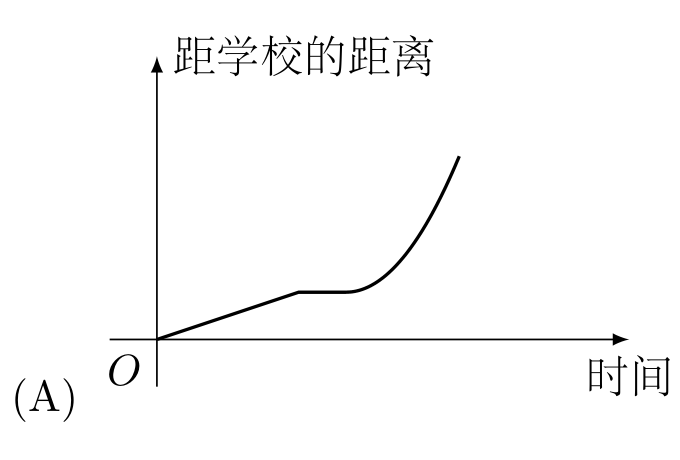
\includegraphics[width=0.15\paperwidth]{GaoKao/images/2013/hubei_liberal/q5_choice_a.png}  &  \text{B. }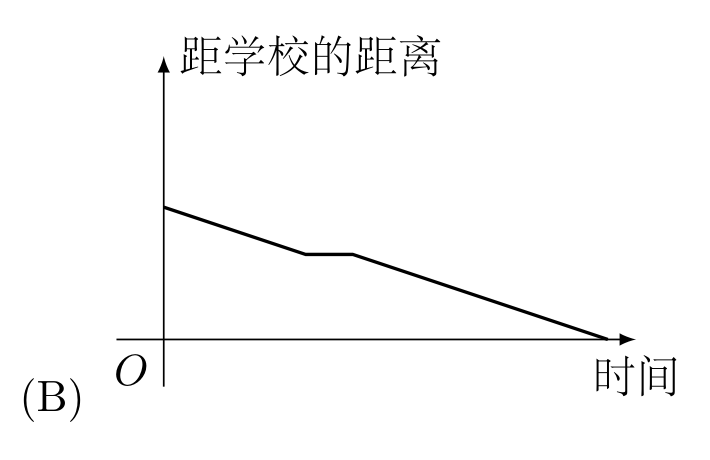
\includegraphics[width=0.15\paperwidth]{GaoKao/images/2013/hubei_liberal/q5_choice_b.png}  &  \text{C. }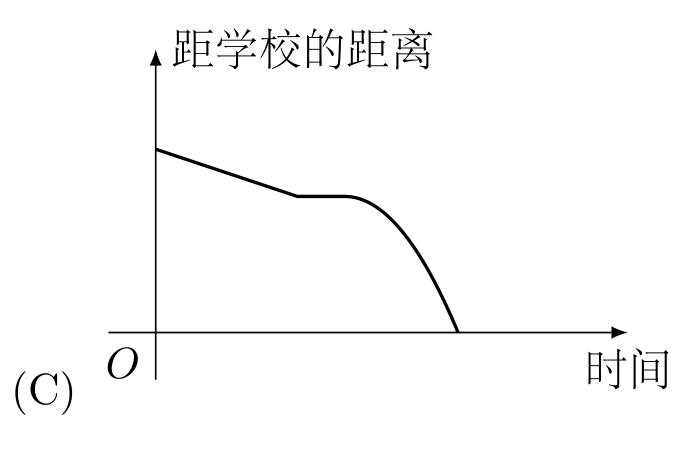
\includegraphics[width=0.15\paperwidth]{GaoKao/images/2013/hubei_liberal/q5_choice_c.png}  &  \text{D. }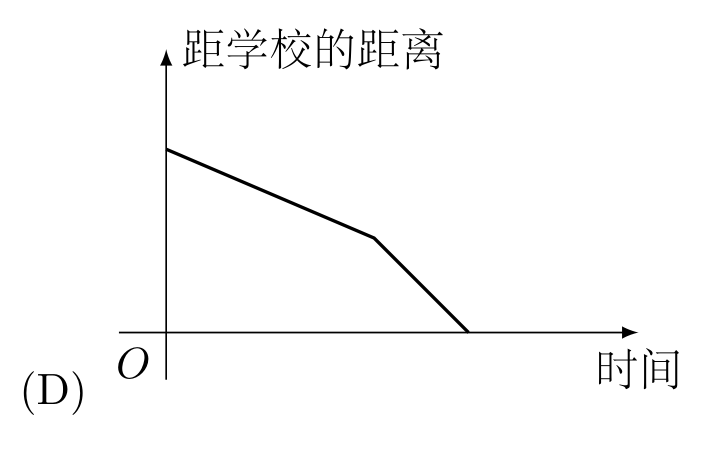
\includegraphics[width=0.15\paperwidth]{GaoKao/images/2013/hubei_liberal/q5_choice_d.png}
        \end{tabular*}\par}

        \item 将函数 \(y=\sqrt{3}\cos x+\sin x\)（\(x\in\mathbb{R}\)）的图象向左平移 \(m\)（\(m>0\)）个单位长度后，所得到的图象关于 \(y\) 轴对称，则 \(m\) 的最小值是（\quad）

        {\centering\begin{tabular*}{\linewidth}{@{}@{\extracolsep{\fill}}llll@{}}
          \text{A. }\(\frac{\pi}{12}\)  &  \text{B. }\(\frac{\pi}{6}\)  &  \text{C. }\(\frac{\pi}{3}\)  &  \text{D. }\(\frac{5\pi}{6}\)
        \end{tabular*}\par}

        \item 已知点 \(A(-1,1)\)，\(B(1,2)\)，\(C(-2,-1)\)，\(D(3,4)\)，则向量 \(\overrightarrow{AB}\) 在 \(\overrightarrow{CD}\) 方向上的投影为（\quad）

        {\centering\begin{tabular*}{\linewidth}{@{}@{\extracolsep{\fill}}llll@{}}
          \text{A. }\(\frac{3\sqrt{2}}{2}\)  &  \text{B. }\(\frac{3\sqrt{15}}{2}\)  &  \text{C. }\(-\frac{3\sqrt{2}}{2}\)  &  \text{D. }\(-\frac{3\sqrt{15}}{2}\)
        \end{tabular*}\par}

        \item \(x\) 为实数， \([x]\) 表示不超过 \(x\) 的最大整数，则函数 \(f(x) = x - [x]\) 在 \(\mathbb{R}\) 上为（\quad）

        {\centering\begin{tabular*}{\linewidth}{@{}@{\extracolsep{\fill}}llll@{}}
          \text{A. }奇函数  &  \text{B. }偶函数  &  \text{C. }增函数  &  \text{D. }周期函数
        \end{tabular*}\par}

        \item 某旅行社租用 \(A\)，\(B\) 两种型号的客车安排 900 名客人旅行，\(A\)，\(B\) 两种车辆的载客量分别为 36 人和 60 人，租金分别为 1600 元/辆和 2400 元/辆. 旅行社要求租车总数不超过 21 辆，且 \(B\) 型车不多于 \(A\) 型车 7 辆，则租金最少为（\quad）

        {\centering\begin{tabular*}{\linewidth}{@{}@{\extracolsep{\fill}}llll@{}}
          \text{A. }31200 元  &  \text{B. }36000 元  &  \text{C. }36800 元  &  \text{D. }38400 元
        \end{tabular*}\par}

        \item 已知函数 \( f(x) = x (\ln x - ax) \) 有两个极值点，则实数 \( a \) 的取值范围是（\quad）

        {\centering\begin{tabular*}{\linewidth}{@{}@{\extracolsep{\fill}}llll@{}}
          \text{A. }\( (-\infty,0) \)  &  \text{B. }\( \left(0,\frac{1}{2}\right) \)  &  \text{C. }\( (0,1) \)  &  \text{D. }\( (0,+\infty) \)
        \end{tabular*}\par}

    \end{enumerate}

\end{description}

\begin{description}

    \item[二、填空题]

    \begin{enumerate}[leftmargin=5pt]

      \addtocounter{enumi}{+10}

        \item \(\i\) 为虚数单位，设复数 \(z_1\)，\(z_2\) 在复平面内对应的点关于原点对称，若 \(z_1=2-3\i\)，则 \(z_2=\)\rule[-0.3ex]{3em}{0.4pt}.

        \item 某学员在一次射击测试中射靶 10 次，命中环数如下：\(7\)，\(8\)，\(7\)，\(9\)，\(5\)，\(4\)，\(9\)，\(10\)，\(7\)，\(4\).
则
\begin{enumerate}
\item 平均命中环数为\rule[-0.3ex]{3em}{0.4pt}；
\item 命中环数的标准差为\rule[-0.3ex]{3em}{0.4pt}.
\end{enumerate}

        \item 阅读如图所示的程序框图，运行相应的程序，若输入 \(m\) 的值为 \(2\)，则输出的结果 \(i=\)\rule[-0.3ex]{3em}{0.4pt}.

\begin{center}
\begin{center}
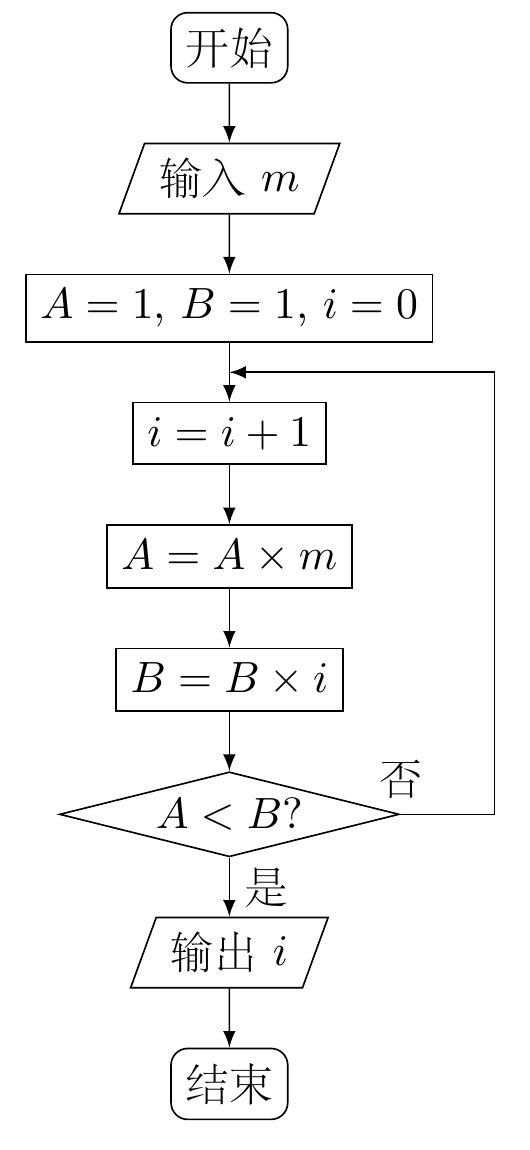
\includegraphics[width=0.48\linewidth]{GaoKao/images/2013/hubei_liberal/q13_fig1.png}
\end{center}
\end{center}

        \item 已知圆 \(O: x^{2} + y^{2} = 5\)，直线 \(l: x \cos \theta + y \sin \theta = 1\)（\(0 < \theta < \frac{\pi}{2}\)）. 设圆 \(O\) 上到直线 \(l\) 的距离等于 1 的点的个数为 \(k\)，则 \(k = \)\rule[-0.3ex]{3em}{0.4pt}.

        \item 在区间 \([-2, 4]\) 上随机地取一个数 \(x\)，若 \(x\) 满足 \(|x| \leqslant m\) 的概率为 \(\frac{5}{6}\)，则 \(m = \)\rule[-0.3ex]{3em}{0.4pt}.

        \item 我国古代数学名著《数书九章》中有“天池盆测雨”题：在下雨时，用一个圆台形的天池盆接雨水，天池盆盆口直径为二尺八寸，盆底直径为一尺二寸，盆深一尺八寸，若盆中积水深九寸，则平地降雨量是\rule[-0.3ex]{3em}{0.4pt}\(\text{寸}\).

注：
\begin{enumerate}
\item 平地降雨量等于盆中积水体积除以盆口面积；
\item 一尺等于十寸.
\end{enumerate}

        \item 在平面直角坐标系中，若点 \(P(x,y)\) 的坐标 \(x\)，\(y\) 均为整数，则称点 \(P\) 为格点，若一个多边形的顶点全是格点，则称该多边形为格点多边形，格点多边形的面积为 \(S\)，其内部的格点数记为 \(N\)，边界上的格点数记为 \(L\). 例如图中 \(\triangle ABC\) 是格点三角形，对应的 \(S=1\)，\(N=0\)，\(L=4\).

\begin{enumerate}
\item 图中格点四边形 \(DEFG\) 对应的 \(S\)，\(N\)，\(L\) 分别是\rule[-0.3ex]{3em}{0.4pt}；
\item 已知格点多边形的面积可表示为 \(S=aN+bL+c\)，其中 \(a\)，\(b\)，\(c\) 为常数. 若某格点多边形对应的 \(N=71\)，\(L=18\)，则 \(S=\)\rule[-0.3ex]{3em}{0.4pt}. （用数值作答）
\end{enumerate}

\begin{center}
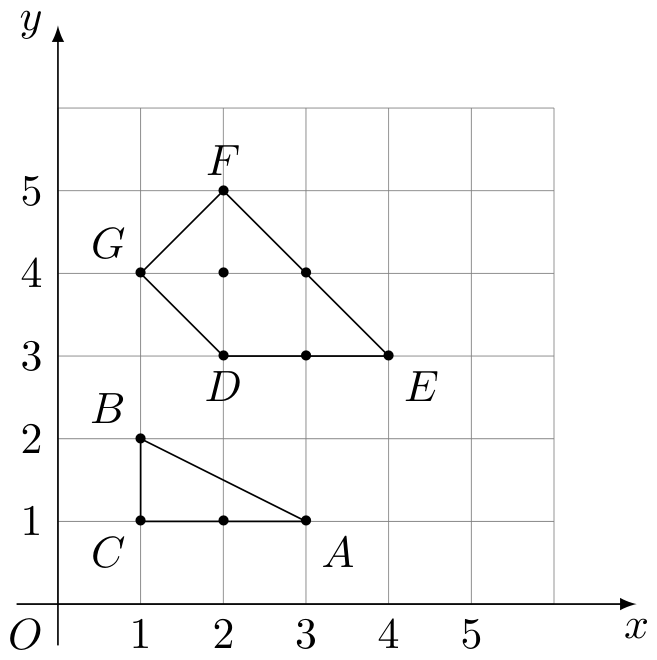
\includegraphics[width=6.5cm]{GaoKao/images/2013/hubei_liberal/q17_fig1.png}
\end{center}

    \end{enumerate}

\end{description}

\begin{description}

    \item[三、解答题]

    \begin{enumerate}[leftmargin=5pt]

      \addtocounter{enumi}{+17}

        \item 在 \(\triangle ABC\) 中，角 \(A\)，\(B\)，\(C\) 对应的边分别是 \(a\)，\(b\)，\(c\)，已知 \(\cos 2A-3\cos(B+C)=1\).

\begin{enumerate}
\item 求角 \(A\) 的大小；
\item 若 \(\triangle ABC\) 的面积 \(S=5\sqrt{3}\)，\(b=5\)，求 \(\sin B\sin C\) 的值.
\end{enumerate}

        \item 已知 \(S_n\) 是等比数列 \(\{a_n\}\) 的前 \(n\) 项和，\(S_4\)，\(S_2\)，\(S_3\) 成等差数列，且 \(a_2+a_3+a_4=-18\).

\begin{enumerate}
\item 求数列 \(\{a_n\}\) 的通项公式；
\item 是否存在正整数 \(n\)，使得 \(S_n\geqslant 2013\)？若存在，求出符合条件的所有 \(n\) 的集合；若不存在，说明理由.
\end{enumerate}

        \item 设 \(a>0\)，\(b>0\)，已知函数 \(f(x)=\frac{ax+b}{x+1}\).

\begin{enumerate}
\item 当 \(a\neq b\) 时，讨论函数 \(f(x)\) 的单调性；
\item 当 \(x>0\) 时，称 \(f(x)\) 为 \(a\)，\(b\) 关于 \(x\) 的加权平均数.
\begin{enumerate}
\item 判断 \(f(1)\)，\(f\left(\sqrt{\frac{b}{a}}\right)\)，\(f\left(\frac{b}{a}\right)\) 是否成等比数列，并证明 \(f\left(\frac{b}{a}\right)\leqslant f\left(\sqrt{\frac{b}{a}}\right)\)；
\item \(a\)，\(b\) 的几何平均数记为 \(G\)，称 \(\frac{2ab}{a+b}\) 为 \(a\)，\(b\) 的调和平均数，记为 \(H\)，若 \(H\leqslant f(x)\leqslant G\)，求 \(x\) 的取值范围.
\end{enumerate}
\end{enumerate}

        \item 如图，某地质队自水平地面 \(A\)，\(B\)，\(C\) 三处垂直向地下钻探，自 \(A\) 点向下钻到 \(A_1\) 处发现矿藏，再继续下钻到 \(A_2\) 处后下面已无矿，从而得到在 \(A\) 处正下方的矿层厚度为 \(A_1A_2=d_1\)，同样可得在 \(B\)，\(C\) 处正下方的矿层厚度分别为 \(B_1B_2=d_2\)，\(C_1C_2=d_3\)，且 \(d_1<d_2<d_3\)，过 \(AB\)，\(AC\) 的中点 \(M\)，\(N\) 且与直线 \(AA_2\) 平行的平面截多面体 \(A_1B_1C_1-A_2B_2C_2\) 所得的截面 \(DEFG\) 为该多面体的一个中截面，其面积记为 \(S_{\text{中}}\).

\begin{enumerate}
\item 证明：中截面 \(DEFG\) 是梯形；
\item 在 \(\triangle ABC\) 中，记 \(BC=a\)，\(BC\) 边上的高为 \(h\)，面积为 \(S\). 在估测三角形 \(ABC\) 区域内正下方的矿藏储量（即多面体 \(A_1B_1C_1-A_2B_2C_2\) 的体积 \(V\)）时，可用近似公式 \(V_{\text{估}}=S_{\text{中}}\cdot h\) 来估算. 已知 \(V=\frac{1}{3}(d_1+d_2+d_3)S\)，试判断 \(V_{\text{估}}\) 与 \(V\) 的大小关系，并加以证明.
\end{enumerate}

\begin{center}
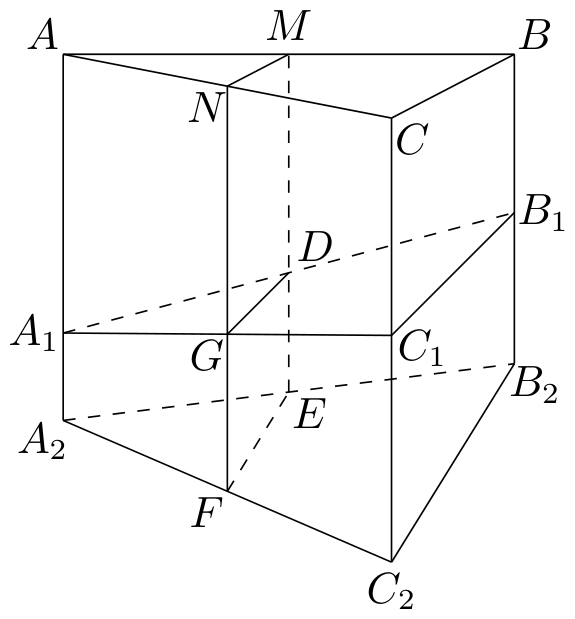
\includegraphics[width=5.8cm]{GaoKao/images/2013/hubei_liberal/q20_fig1.png}
\end{center}

        \item 如图，已知椭圆 \(C_1\) 与 \(C_2\) 的中心在坐标原点 \(O\)，长轴均为 \(MN\) 且在 \(x\) 轴上，短轴长分别为 \(2m\)，\(2n\)（\(m>n\)），过原点且不与 \(x\) 轴重合的直线 \(l\) 与 \(C_1\)，\(C_2\) 的四个交点按纵坐标从大到小依次为 \(A\)，\(B\)，\(C\)，\(D\)，记 \(\lambda=\frac{m}{n}\)，\(\triangle BDM\) 和 \(\triangle ABN\) 的面积分别为 \(S_1\) 和 \(S_2\).

\begin{enumerate}
\item 当直线 \(l\) 与 \(y\) 轴重合时，若 \(S_1=\lambda S_2\)，求 \(\lambda\) 的值；
\item 当 \(\lambda\) 变化时，是否存在与坐标轴不重合的直线 \(l\)，使得 \(S_1=\lambda S_2\)？并说明理由.
\end{enumerate}

\begin{center}
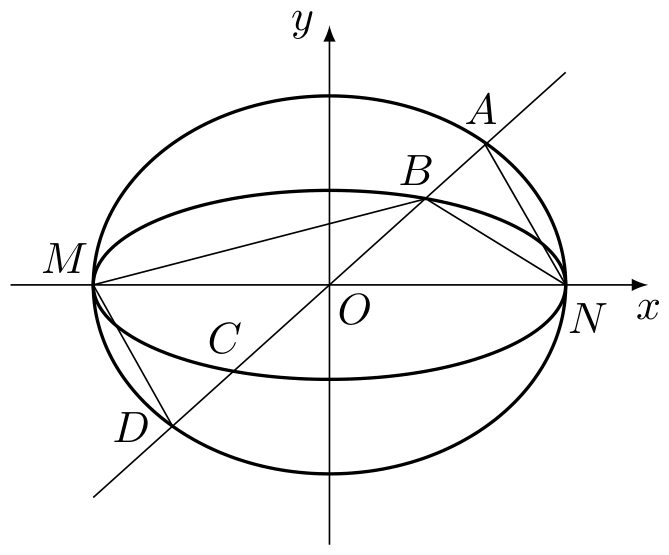
\includegraphics[width=8.0cm]{GaoKao/images/2013/hubei_liberal/q22_fig1.png}
\end{center}

    \end{enumerate}

\end{description}


\subsection{2013年湖南卷（理）}\label{gk:2013年湖南卷（理）}

\begin{description}

    \item[一、选择题]

    \begin{enumerate}[leftmargin=5pt]

        \item 复数 \(z = \i \cdot (1 + \i)\)（\(\i\) 为虚数单位）在复平面上对应的点位于（\quad）

        {\centering\begin{tabular*}{\linewidth}{@{}@{\extracolsep{\fill}}llll@{}}
          \text{A. }第一象限  &  \text{B. }第二象限  &  \text{C. }第三象限  &  \text{D. }第四象限
        \end{tabular*}\par}

        \item 某学校有男、女学生各 \(500\text{ 名}\). 为了解男女学生在学习兴趣与业余爱好方面是否存在显著差异，拟从全体学生中抽取 \(100\text{ 名}\)学生进行调查，则宜采用的抽样方法是（\quad）

        {\centering\begin{tabular*}{\linewidth}{@{}@{\extracolsep{\fill}}llll@{}}
          \text{A. }抽签法  &  \text{B. }随机数法  &  \text{C. }系统抽样法  &  \text{D. }分层抽样法
        \end{tabular*}\par}

        \item 在锐角 \(\triangle ABC\) 中，角 \(A\)，\(B\) 所对的边长分别为 \(a\)，\(b\). 若 \(2a \sin B = \sqrt{3} b\)，则角 \(A\) 等于（\quad）

        {\centering\begin{tabular*}{\linewidth}{@{}@{\extracolsep{\fill}}llll@{}}
          \text{A. }\( \frac{\pi}{12} \)  &  \text{B. }\( \frac{\pi}{6} \)  &  \text{C. }\( \frac{\pi}{4} \)  &  \text{D. }\(\frac{\pi}{3}\)
        \end{tabular*}\par}

        \item 若变量 \(x\)，\(y\) 满足的约束条件 \(\begin{cases}
y \leqslant 2x,\\
x + y \leqslant 1,\\
y \geqslant -1,
\end{cases}\) 则 \(x + 2y\) 的最大值是（\quad）

        {\centering\begin{tabular*}{\linewidth}{@{}@{\extracolsep{\fill}}llll@{}}
          \text{A. }\(-\frac{5}{2}\)  &  \text{B. }0  &  \text{C. }\( \frac{5}{3} \)  &  \text{D. }\( \frac{5}{2} \)
        \end{tabular*}\par}

        \item 函数 \( f(x) = 2\ln x \) 的图象与函数 \( g(x) = x^2 - 4x + 5 \) 的图象的交点个数为（\quad）

        {\centering\begin{tabular*}{\linewidth}{@{}@{\extracolsep{\fill}}llll@{}}
          \text{A. }3  &  \text{B. }2  &  \text{C. }1  &  \text{D. }0
        \end{tabular*}\par}

        \item 已知 \(\bm{a}\)，\(\bm{b}\) 是单位向量，\(\bm{a} \cdot \bm{b} = 0\). 若向量 \(\bm{c}\) 满足 \(\left|\bm{c} - \bm{a} - \bm{b}\right| = 1\)，则 \(\left|\bm{c}\right|\) 的取值范围是（\quad）

        {\centering\begin{tabular*}{\linewidth}{@{}@{\extracolsep{\fill}}llll@{}}
          \text{A. }\(\left[\sqrt{2} - 1, \sqrt{2} + 1\right]\)  &  \text{B. }\(\left[\sqrt{2} - 1, \sqrt{2} + 2\right]\)  &  \text{C. }\([1, \sqrt{2} + 1]\)  &  \text{D. }\([1, \sqrt{2} + 2]\)
        \end{tabular*}\par}

        \item 已知棱长为 \(1\) 的正方体的俯视图是一个面积为 \(1\) 的正方形，则该正方体的正视图的面积不可能等于（\quad）

        {\centering\begin{tabular*}{\linewidth}{@{}@{\extracolsep{\fill}}llll@{}}
          \text{A. }1  &  \text{B. }\(\sqrt{2}\)  &  \text{C. }\(\frac{\sqrt{2} - 1}{2}\)  &  \text{D. }\(\frac{\sqrt{2} + 1}{2}\)
        \end{tabular*}\par}

        \item 在等腰直角三角形 \(ABC\) 中，\(AB = AC = 4\)，点 \(P\) 是边 \(AB\) 上异于 \(A\)，\(B\) 的一点，光线从点 \(P\) 出发，经 \(BC\)，\(CA\) 反射后又回到点 \(P\) （如图）. 若光线 \(QR\) 经过 \(\triangle ABC\) 的重心，则 \(AP\) 等于（\quad）

        {\centering\begin{tabular*}{\linewidth}{@{}@{\extracolsep{\fill}}llll@{}}
          \text{A. }2  &  \text{B. }1  &  \text{C. }\( \frac{8}{3} \)  &  \text{D. }\( \frac{4}{3} \)
        \end{tabular*}\par}

    \end{enumerate}

\end{description}

\begin{description}

    \item[二、填空题]

    \begin{enumerate}[leftmargin=5pt]

      \addtocounter{enumi}{+8}

        \item 在平面直角坐标系 \(xOy\) 中，若直线 \(l: \begin{cases}
x = t,\\
y = t - a,
\end{cases}\)（\(t\) 为参数）过椭圆 \(C: \begin{cases}
x = 3\cos \varphi,\\
y = 2\sin \varphi.
\end{cases}\)（\(\varphi\) 为参数）的右顶点，则常数 \(a\) 的值为\rule[-0.3ex]{3em}{0.4pt}.

        \item 已知 \(a\)，\(b\)，\(c \in \mathbb{R}\)，\(a + 2b + 3c = 6\)，则 \(a^2 + 4b^2 + 9c^2\) 的最小值为\rule[-0.3ex]{3em}{0.4pt}.

        \item 如图，在半径为 \(\sqrt{7}\) 的 \(\odot O\) 中，弦 \(AB\)，\(CD\) 相交于点 \(P\)，\(PA = PB = 2\)，\(PD = 1\)，则圆心 \(O\) 到弦 \(CD\) 的距离为\rule[-0.3ex]{3em}{0.4pt}.
\begin{center}
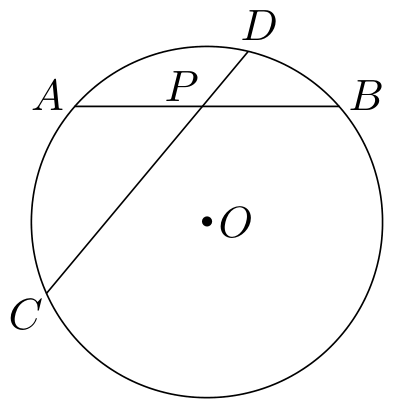
\includegraphics[width=3.9cm]{GaoKao/images/2013/hunan_science/q11_fig1.png}
\end{center}

        \item 若 \(\int_{0}^{T} x^{2} \mathrm{d}x = 9\)，则常数 \(T\) 的值为\rule[-0.3ex]{3em}{0.4pt}.

        \item 执行如图所示的程序框图，如果输入 \(a = 1\)，\(b = 2\)，则输出的 \(a\) 的值为\rule[-0.3ex]{3em}{0.4pt}.
\begin{center}
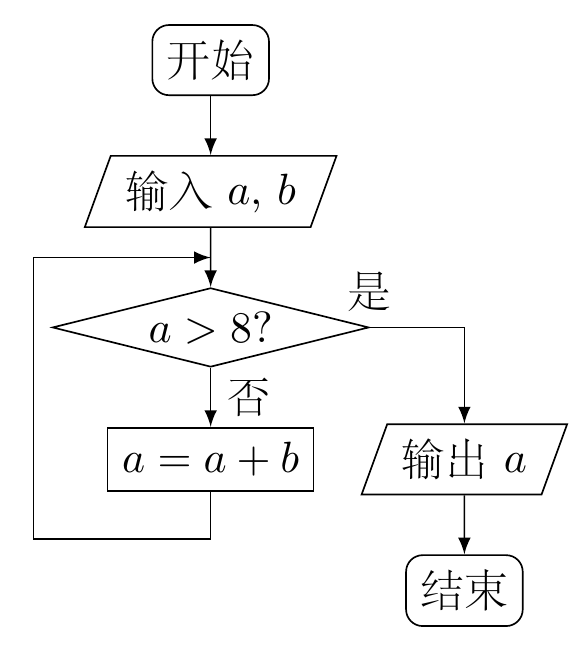
\includegraphics[width=0.60\linewidth]{GaoKao/images/2013/hunan_science/q13_fig1.png}
\end{center}

        \item 设 \(F_{1}\)，\(F_{2}\) 是双曲线 \(C: \frac{x^{2}}{a^{2}} - \frac{y^{2}}{b^{2}} = 1 \) （\(a > 0, b > 0\)）的两个焦点，\(P\) 是 \(C\) 上一点，若 \(|PF_{1}| + |PF_{2}| = 6a\)，且 \(\triangle PF_{1}F_{2}\) 的最小内角为 \(30^{\circ}\)，则 \(C\) 的离心率为\rule[-0.3ex]{3em}{0.4pt}.

        \item 设 \(S_{n}\) 为数列 \(\{a_{n}\}\) 的前 \(n\) 项和，\(S_{n} = (-1)^{n}a_{n} - \frac{1}{2^{n}}\)，\(n \in \mathbb{N}^{*}\)，则
\begin{enumerate}
\item \(a_{3} =\rule[-0.3ex]{3em}{0.4pt}\)；
\item \(S_{1} + S_{2} + \dots + S_{100} =\rule[-0.3ex]{3em}{0.4pt}\).
\end{enumerate}

        \item 设函数 \(f(x) = a^x + b^x - c^x\)，其中 \(c > a > 0\)，\(c > b > 0\).
\begin{enumerate}
\item 记集合 \(M = \{(a, b, c) \mid a, b, c\) 不能构成一个三角形的三条边长，且 \(a = b\}\)，则 \((a, b, c) \in M\) 所对应的 \(f(x)\) 的零点的取值集合为\rule[-0.3ex]{3em}{0.4pt}；
\item 若 \(a\)，\(b\)，\(c\) 是 \(\triangle ABC\) 的三条边长，则下列结论正确的是\rule[-0.3ex]{3em}{0.4pt}.（写出所有正确结论的序号）
\begin{enumerate}
\item \(\forall x \in (-\infty, 1)\)，\(f(x) > 0\)；
\item \(\exists x \in \mathbb{R}\)，使 \(a^{x}\)，\(b^{x}\)，\(c^{x}\) 不能构成一个三角形的三条边长；
\item 若 \(\triangle ABC\) 为钝角三角形，则 \(\exists x \in (1, 2)\)，使 \(f(x) = 0\).
\end{enumerate}
\end{enumerate}

    \end{enumerate}

\end{description}

\begin{description}

    \item[三、解答题]

    \begin{enumerate}[leftmargin=5pt]

      \addtocounter{enumi}{+16}

        \item 已知函数 \(f(x) = \sin \left(x - \frac{\pi}{6}\right) + \cos \left(x - \frac{\pi}{3}\right)\)，\(g(x) = 2\sin^2\frac{x}{2}\).
\begin{enumerate}
\item 若 \(\alpha\) 是第一象限角，且 \(f(\alpha) = \frac{3\sqrt{3}}{5}\)，求 \(g(\alpha)\) 的值；
\item 求使 \( f(x) \geqslant g(x) \) 成立的 \( x \) 的取值集合.
\end{enumerate}

        \item 某人在如图所示的直角边长为 \(4\text{ 米}\) 的三角形地块的每个格点（指纵、横直线的交叉点以及三角形的顶点）处都种了一株相同品种的作物. 根据历年的种植经验，一株该种作物的年收获量 \(Y\)（单位：\(\mathrm{kg}\)）与它的“相近”作物株数 \(X\) 之间的关系如下表所示：

\begin{center}
\begin{tabular}{c|cccc}
\(X\) & 1 & 2 & 3 & 4 \\
\hline
\(Y\) & 51 & 48 & 45 & 42
\end{tabular}
\end{center}

这里，两株作物“相近”是指它们之间的直线距离不超过 \(1\text{ 米}\).

\begin{enumerate}
\item 从三角形地块的内部和边界上分别随机选取一株作物，求它们恰好“相近”的概率；
\item 从所种作物中随机选取一株，求它的年收获量的分布列与数学期望.
\end{enumerate}

\begin{center}
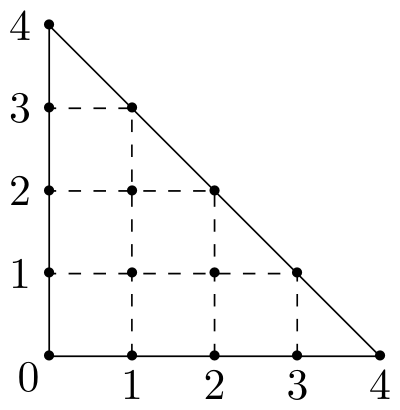
\includegraphics[width=4.0cm]{GaoKao/images/2013/hunan_science/q18_fig1.png}
\end{center}

        \item 如图，在直棱柱 \(ABCD - A_{1}B_{1}C_{1}D_{1}\) 中，\(AD \parallel BC\)，\(\angle BAD = 90^{\circ}\)，\(AC \perp BD\)，\(BC = 1\)，\(AD = AA_{1} = 3\).
\begin{enumerate}
\item 证明： \(AC \perp B_{1}D_{1}\)；
\item 求直线 \(B_{1}C_{1}\) 与平面 \(ACD_{1}\) 所成角的正弦值.
\end{enumerate}
\begin{center}
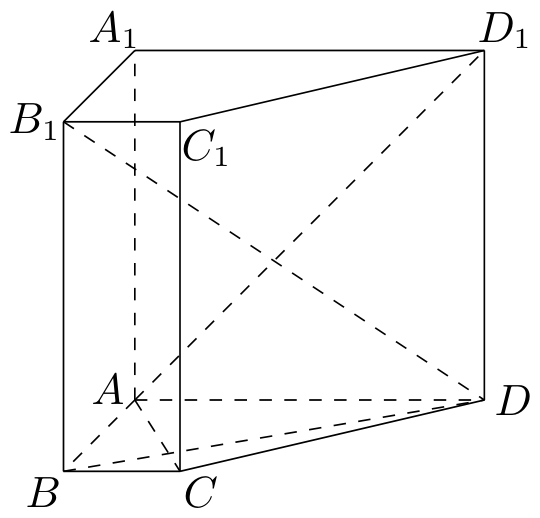
\includegraphics[width=5.4cm]{GaoKao/images/2013/hunan_science/q19_fig1.png}
\end{center}

        \item 在平面直角坐标系 \(xOy\) 中，将从点 \(M\) 出发沿纵、横方向到达点 \(N\) 的任一路径称为 \(M\) 到 \(N\) 的一条“\(L\) 路径”. 如图所示的路径 \(MM_{1}M_{2}M_{3}N\) 与路径 \(MN_{1}N\) 都是 \(M\) 到 \(N\) 的“\(L\) 路径”. 某地有三个新建的居民区，分别位于平面 \(xOy\) 内三点 \(A(3,20)\)，\(B(-10,0)\)，\(C(14,0)\) 处. 现计划在 \(x\) 轴上方区域（包含 \(x\) 轴）内的某一点 \(P\) 处修建一个文化中心.
\begin{enumerate}
\item 写出点 \(P\) 到居民区 \(A\) 的“\(L\) 路径”长度最小值的表达式（不要求证明）；
\item 若以原点 \(O\) 为圆心，半径为 \(1\) 的圆的内部是保护区，“\(L\) 路径”不能进入保护区，请确定点 \(P\) 的位置，使其到三个居民区的“\(L\) 路径”长度之和最小.
\end{enumerate}
\begin{center}
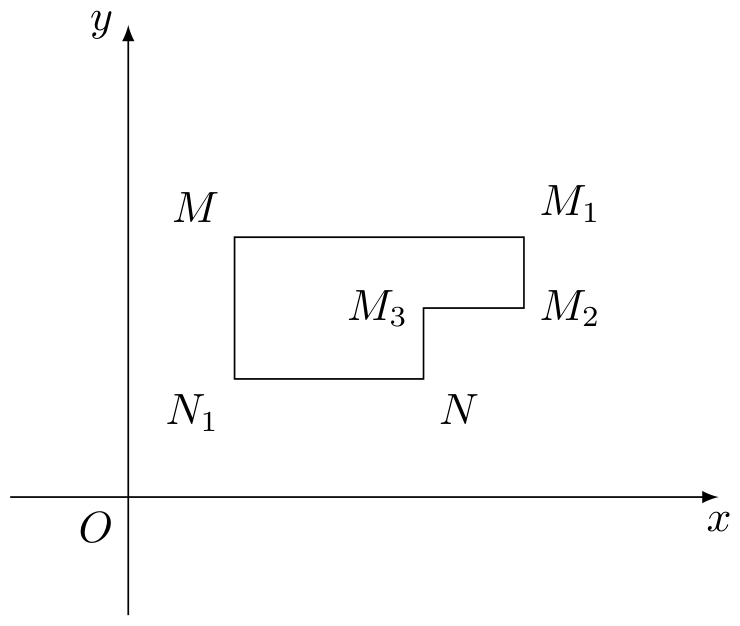
\includegraphics[width=7.5cm]{GaoKao/images/2013/hunan_science/q20_fig1.png}
\end{center}

        \item 过抛物线 \(E: x^{2} = 2py\)（\(p > 0\)）的焦点 \(F\) 作斜率分别为 \(k_{1}\)，\(k_{2}\) 的两条不同的直线 \(l_{1}\)，\(l_{2}\)，且 \(k_{1} + k_{2} = 2\)，\(l_{1}\) 与 \(E\) 相交于点 \(A\)，\(B\)，\(l_{2}\) 与 \(E\) 相交于点 \(C\)，\(D\). 以 \(AB\)，\(CD\) 为直径的圆 \(M\)，圆 \(N\)（\(M\)，\(N\) 为圆心）的公共弦所在的直线记为 \(l\).
\begin{enumerate}
\item 若 \(k_{1} > 0\)，\(k_{2} > 0\)，证明：\(\overrightarrow{FM} \cdot \overrightarrow{FN} < 2p^{2}\)；
\item 若点 \(M\) 到直线 \(l\) 的距离的最小值为 \(\frac{7\sqrt{5}}{5}\)，求抛物线 \(E\) 的方程.
\end{enumerate}

        \item 已知 \(a > 0\)，函数 \(f(x) = \left| \frac{x - a}{x + 2a} \right|\).
\begin{enumerate}
\item 记 \(f(x)\) 在区间 \([0, 4]\) 上的最大值为 \(g(a)\)，求 \(g(a)\) 的表达式；
\item 是否存在 \(a\)，使函数 \(y = f(x)\) 在区间 \((0, 4)\) 内的图象上存在两点，在该两点处的切线相互垂直？若存在，求 \(a\) 的取值范围；若不存在，请说明理由.
\end{enumerate}

    \end{enumerate}

\end{description}


\subsection{2013年湖南卷（文）}\label{gk:2013年湖南卷（文）}

\begin{description}

    \item[一、选择题]

    \begin{enumerate}[leftmargin=5pt]

        \item 复数 \(z = \i \cdot (1 + \i)\) （\(\i\) 为虚数单位）在复平面上对应的点位于（\quad）

        {\centering\begin{tabular*}{\linewidth}{@{}@{\extracolsep{\fill}}llll@{}}
          \text{A. }第一象限  &  \text{B. }第二象限  &  \text{C. }第三象限  &  \text{D. }第四象限
        \end{tabular*}\par}

        \item “\(1 < x < 2\)”是“\(x < 2\)”成立的（\quad）

        {\centering\begin{tabular*}{\linewidth}{@{}@{\extracolsep{\fill}}llll@{}}
          \text{A. }充分不必要条件  &  \text{B. }必要不充分条件  &  \text{C. }充分必要条件  &  \text{D. }既不充分也不必要条件
        \end{tabular*}\par}

        \item 某工厂甲，乙，丙三个车间生产了同一种产品，数量分别为 \(120\text{ 件}\)，\(80\text{ 件}\)，\(60\text{ 件}\). 为了解它们的产品质量是否存在显著差异，用分层抽样方法抽取了一个容量为 \(n\) 的样本进行调查，其中从丙车间的产品中抽取了 \(3\text{ 件}\)，则 \(n=\)（\quad）

        {\centering\begin{tabular*}{\linewidth}{@{}@{\extracolsep{\fill}}llll@{}}
          \text{A. }9  &  \text{B. }10  &  \text{C. }12  &  \text{D. }13
        \end{tabular*}\par}

        \item 已知 \( f(x) \) 是奇函数，\( g(x) \) 是偶函数，且 \( f(-1)+g(1)=2 \)，\( f(1)+g(-1)=4 \)，则 \( g(1) \) 等于（\quad）

        {\centering\begin{tabular*}{\linewidth}{@{}@{\extracolsep{\fill}}llll@{}}
          \text{A. }4  &  \text{B. }3  &  \text{C. }2  &  \text{D. }1
        \end{tabular*}\par}

        \item 在锐角 \(\triangle ABC\) 中，角 \(A\)，\(B\) 所对的边长分别为 \(a\)，\(b\). 若 \(2a \sin B = \sqrt{3} b\)，则角 \(A\) 等于（\quad）

        {\centering\begin{tabular*}{\linewidth}{@{}@{\extracolsep{\fill}}llll@{}}
          \text{A. }\( \frac{\pi}{3} \)  &  \text{B. }\( \frac{\pi}{4} \)  &  \text{C. }\( \frac{\pi}{6} \)  &  \text{D. }\( \frac{\pi}{12} \)
        \end{tabular*}\par}

        \item 函数 \( f(x) = \ln x \) 的图象与函数 \( g(x) = x^2 - 4x + 4 \) 的图象的交点个数为（\quad）

        {\centering\begin{tabular*}{\linewidth}{@{}@{\extracolsep{\fill}}llll@{}}
          \text{A. }0  &  \text{B. }1  &  \text{C. }2  &  \text{D. }3
        \end{tabular*}\par}

        \item 已知正方体的棱长为 1，其俯视图是一个面积为 1 的正方形，侧视图是一个面积为 \(\sqrt{2}\) 的矩形，则该正方体的正视图的面积等于（\quad）

        {\centering\begin{tabular*}{\linewidth}{@{}@{\extracolsep{\fill}}llll@{}}
          \text{A. }\(\frac{\sqrt{3}}{2}\)  &  \text{B. }1  &  \text{C. }\(\frac{\sqrt{2} + 1}{2}\)  &  \text{D. }\(\sqrt{2}\)
        \end{tabular*}\par}

        \item 已知 \(\bm{a}\)，\(\bm{b}\) 是单位向量，\(\bm{a} \cdot \bm{b} = 0\). 若向量 \(\bm{c}\) 满足 \(|\bm{c} - \bm{a} - \bm{b}| = 1\)，则 \(|\bm{c}|\) 的最大值为（\quad）

        {\centering\begin{tabular*}{\linewidth}{@{}@{\extracolsep{\fill}}llll@{}}
          \text{A. }\(\sqrt{2} - 1\)  &  \text{B. }\(\sqrt{2}\)  &  \text{C. }\(\sqrt{2} + 1\)  &  \text{D. }\(\sqrt{2} + 2\)
        \end{tabular*}\par}

        \item 已知事件“在矩形 \(ABCD\) 的边 \(CD\) 上随机取一点 \(P\)，使 \(\triangle APB\) 的最大边是 \(AB\)”发生的概率为 \(\frac{1}{2}\)，则 \(\frac{AD}{AB} =\)（\quad）

        {\centering\begin{tabular*}{\linewidth}{@{}@{\extracolsep{\fill}}llll@{}}
          \text{A. }\(\frac{1}{2}\)  &  \text{B. }\(\frac{1}{4}\)  &  \text{C. }\(\frac{\sqrt{3}}{2}\)  &  \text{D. }\(\frac{\sqrt{7}}{4}\)
        \end{tabular*}\par}

    \end{enumerate}

\end{description}

\begin{description}

    \item[二、填空题]

    \begin{enumerate}[leftmargin=5pt]

      \addtocounter{enumi}{+9}

        \item 已知集合 \(U = \{2, 3, 6, 8\}\)，\(A = \{2, 3\}\)，\(B = \{2, 6, 8\}\)，则 \(\complement_U A \cap B =\rule[-0.3ex]{3em}{0.4pt}\).

        \item 在平面直角坐标系 \(xOy\) 中，若直线 \(l_{1}: \begin{cases}
x = 2s + 1,\\
y = s,
\end{cases}\) （\(s\) 为参数）和直线 \(l_{2}: \begin{cases}
x = at,\\
y = 2t - 1,
\end{cases}\) （\(t\) 为参数）平行，则常数 \(a\) 的值为\rule[-0.3ex]{3em}{0.4pt}.

        \item 执行如图所示的程序框图，如果输入 \(a = 1\)，\(b = 2\)，则输出的 \(a\) 的值为\rule[-0.3ex]{3em}{0.4pt}.

\begin{center}
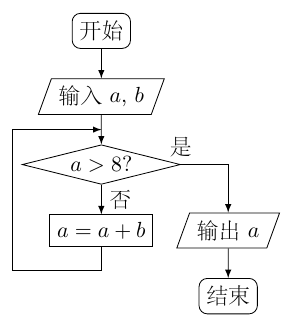
\includegraphics[width=0.46\linewidth]{GaoKao/images/2013/hunan_liberal/q12_fig1.png}
\end{center}

        \item 若变量 \(x\)，\(y\) 满足约束条件 \(\begin{cases}
x + 2y \leqslant 8,\\
0 \leqslant x \leqslant 4,\\
0 \leqslant y \leqslant 3,
\end{cases}\) 则 \(x + y\) 的最大值为\rule[-0.3ex]{3em}{0.4pt}.

        \item 设 \(F_{1}\)，\(F_{2}\) 是双曲线 \(C: \frac{x^{2}}{a^{2}} - \frac{y^{2}}{b^{2}} = 1 \) （\(a > 0, b > 0\)）的两个焦点. 若在 \(C\) 上存在一点 \(P\)，使 \(PF_{1} \perp PF_{2}\)，且 \(\angle PF_{1}F_{2} = 30^{\circ}\)，则 \(C\) 的离心率为\rule[-0.3ex]{3em}{0.4pt}.

        \item 对于 \(E = \{a_1, a_2, \cdots, a_{100}\}\) 的子集 \(X = \{a_{i_1}, a_{i_2}, \cdots, a_{i_k}\}\)，定义 \(X\) 的“特征数列”为 \(x_1\)，\(x_2\)，\(\cdots\)，\(x_{100}\)，其中 \(x_{i_1} = x_{i_2} = \cdots = x_{i_k} = 1\)，其余项均为 \(0\)，例如：子集 \(\{a_2, a_3\}\) 的“特征数列”为 \(0\)，\(1\)，\(1\)，\(0\)，\(0\)，\(\cdots\)，\(0\).
\begin{enumerate}
\item 子集 \( \{a_{1}, a_{3}, a_{5}\} \) 的“特征数列”的前 3 项和等于\rule[-0.3ex]{3em}{0.4pt}.
\item 若 \(E\) 的子集 \(P\) 的“特征数列” \(p_{1}\)，\(p_{2}\)，\(\cdots\)，\(p_{100}\) 满足 \(p_{1}=1\)，\(p_{i}+p_{i+1}=1\)，\(1\leqslant i\leqslant99\)；\(E\) 的子集 \(Q\) 的“特征数列” \(q_{1}\)，\(q_{2}\)，\(\cdots\)，\(q_{100}\) 满足 \(q_{1}=1\)，\(q_{j}+q_{j+1}+q_{j+2}=1\)，\(1\leqslant j\leqslant98\)，则 \(P\cap Q\) 的元素个数为\rule[-0.3ex]{3em}{0.4pt}.
\end{enumerate}

    \end{enumerate}

\end{description}

\begin{description}

    \item[三、解答题]

    \begin{enumerate}[leftmargin=5pt]

      \addtocounter{enumi}{+15}

        \item 已知函数 \( f(x) = \cos x \cdot \cos \left(x - \frac{\pi}{3}\right) \).
\begin{enumerate}
\item 求 \( f\left(\frac{2\pi}{3}\right) \) 的值；
\item 求使 \( f(x) < \frac{1}{4} \) 成立的 \( x \) 的取值集合.
\end{enumerate}

        \item 如图，在直棱柱 \(ABC - A_{1}B_{1}C_{1}\) 中，\(\angle BAC = 90^{\circ}\)，\(AB = AC = \sqrt{2}\)，\(AA_{1} = 3\)，\(D\) 是 \(BC\) 的中点，点 \(E\) 在棱 \(BB_{1}\) 上运动.

\begin{enumerate}
\item 证明：\(AD \perp C_{1}E\)；
\item 当异面直线 \(AC\)，\(C_1E\) 所成的角为 \(60^\circ\) 时，求三棱锥 \(C_1 - A_1B_1E\) 的体积.
\end{enumerate}

\begin{center}
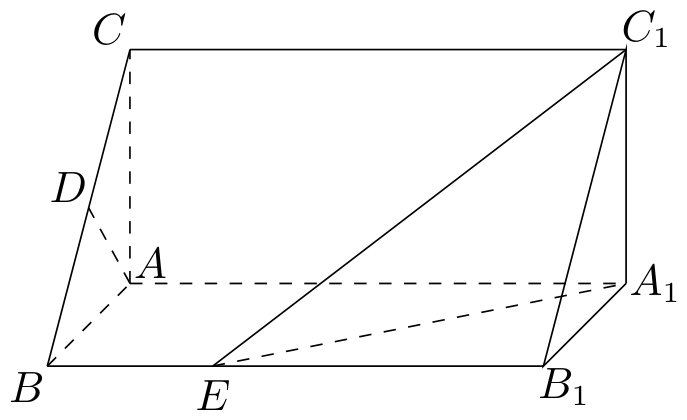
\includegraphics[width=6.9cm]{GaoKao/images/2013/hunan_liberal/q17_fig1.png}
\end{center}

        \item 某人在如图所示的直角边长为 \(4\text{ 米}\) 的三角形地块的每个格点（指纵、横直线的交叉点以及三角形的顶点）处都种了一株相同品种的作物. 根据历年的种植经验，一株该种作物的年收获量 \(Y\)（单位：\(\mathrm{kg}\)）与它的“相近”作物株数 \(X\) 之间的关系如下表所示：
\begin{center}
\begin{tabular}{c|cccc}
\(X\) & \(1\) & \(2\) & \(3\) & \(4\) \\
\hline
\(Y\) & \(51\) & \(48\) & \(45\) & \(42\)
\end{tabular}
\end{center}
这里，两株作物“相近”是指它们之间的直线距离不超过 \(1\text{ 米}\).

\begin{enumerate}
\item 完成下表，并求所种作物的平均年收获量；
\begin{center}
\begin{tabular}{c|cccc}
\(Y\) & \(51\) & \(48\) & \(45\) & \(42\) \\
\hline
频数 &\rule[-0.3ex]{3em}{0.4pt} & \(4\) &\rule[-0.3ex]{3em}{0.4pt} &\rule[-0.3ex]{3em}{0.4pt}
\end{tabular}
\end{center}
\item 在所种作物中随机选取一株，求它的年收获量至少为 \(48 \mathrm{~kg}\) 的概率.
\end{enumerate}

\begin{center}
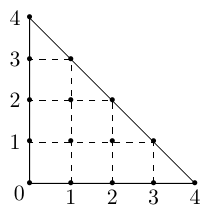
\includegraphics[width=4.1cm]{GaoKao/images/2013/hunan_liberal/q18_fig1.png}
\end{center}

        \item 设 \(S_{n}\) 为数列 \(\{a_{n}\}\) 的前 \(n\) 项和. 已知 \(a_1 \neq 0\)，\(2a_{n} - a_1 = S_1 \cdot S_n\)，\(n \in \mathbb{N}^*\).
\begin{enumerate}
\item 求 \(a_{1}\)，\(a_{2}\)，并求数列 \( \{a_{n}\} \) 的通项公式；
\item 求数列 \( \{na_{n}\} \) 的前 \(n\) 项和.
\end{enumerate}

        \item 已知 \(F_{1}\)，\(F_{2}\) 分别是椭圆 \(E: \frac{x^{2}}{5} + y^{2} = 1\) 的左，右焦点，\(F_{1}\)，\(F_{2}\) 关于直线 \(x + y - 2 = 0\) 的对称点是圆 \(C\) 的一条直径的两个端点.
\begin{enumerate}
\item 求圆 \(C\) 的方程；
\item 设过点 \(F_{2}\) 的直线 \(l\) 被椭圆 \(E\) 和圆 \(C\) 所截得的弦长分别为 \(a\)，\(b\). 当 \(ab\) 最大时，求直线 \(l\) 的方程.
\end{enumerate}

        \item 已知函数 \( f(x) = \frac{1 - x}{1 + x^{2}} {\mathrm{e}}^x \).
\begin{enumerate}
\item 求 \( f(x) \) 的单调区间；
\item 证明：当 \( f(x_{1}) = f(x_{2})  \) （\(x_{1} \neq x_{2}\)）时，\( x_{1} + x_{2} < 0 \).
\end{enumerate}

    \end{enumerate}

\end{description}


\subsection{2013年江苏卷}\label{gk:2013年江苏卷}

\begin{description}

    \item[一、填空题]

    \begin{enumerate}[leftmargin=5pt]

        \item 函数 \(y=3\sin\left(2x+\frac{\pi}{4}\right)\) 的最小正周期为\rule[-0.3ex]{3em}{0.4pt}.

        \item 设 \(z=(2-\i)^2\)（\(\i\) 为虚数单位），则复数 \(z\) 的模为\rule[-0.3ex]{3em}{0.4pt}.

        \item 双曲线 \(\frac{x^2}{16}-\frac{y^2}{9}=1\) 的两条渐近线的方程为\rule[-0.3ex]{3em}{0.4pt}.

        \item 集合 \(\{-1,0,1\}\) 共有\rule[-0.3ex]{3em}{0.4pt} 个子集.

        \item 如图是一个算法的流程图，则输出的 \(n\) 的值是\rule[-0.3ex]{3em}{0.4pt}.

\begin{center}
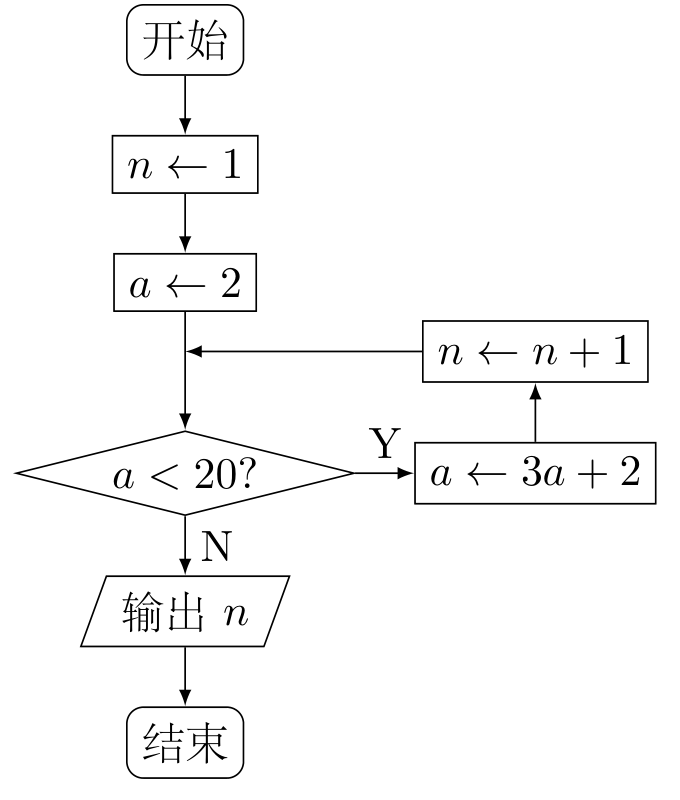
\includegraphics[width=0.34\linewidth]{GaoKao/images/2013/jiangsu/q5_fig1.png}
\end{center}

        \item 抽样统计甲，乙两位射击运动员的 \(5\) 次训练成绩（单位：环），结果如下：

\begin{center}
{\renewcommand{\arraystretch}{1.15}
\begin{tabular}{|c|c|c|c|c|c|}
\hline
运动员 & 第1次 & 第2次 & 第3次 & 第4次 & 第5次 \\
\hline
甲 & 87 & 91 & 90 & 89 & 93 \\
\hline
乙 & 89 & 90 & 91 & 88 & 92 \\
\hline
\end{tabular}}
\end{center}

则成绩较为稳定（方差较小）的那位运动员成绩的方差为\rule[-0.3ex]{3em}{0.4pt}.

        \item 现有某类病毒记作 \(X_mY_n\)，其中正整数 \(m\)，\(n\)（\(m\leqslant 7\)，\(n\leqslant 9\)）可以任意选取，则 \(m\)，\(n\) 都取到奇数的概率为\rule[-0.3ex]{3em}{0.4pt}.

        \item 如图，在三棱柱 \(A_1B_1C_1-ABC\) 中，\(D\)，\(E\)，\(F\) 分别是 \(AB\)，\(AC\)，\(AA_1\) 的中点. 设三棱锥 \(F-ADE\) 的体积为 \(V_1\)，三棱柱 \(A_1B_1C_1-ABC\) 的体积为 \(V_2\)，则 \(V_1:V_2=\rule[-0.3ex]{3em}{0.4pt}\).

\begin{center}
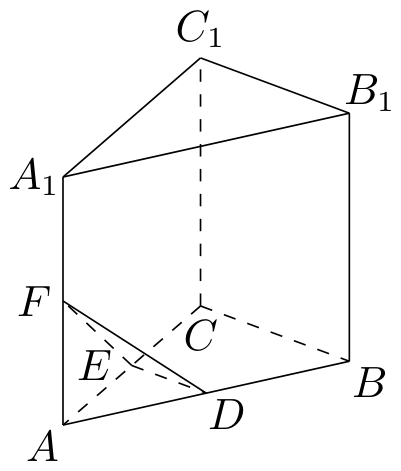
\includegraphics[width=4.7cm]{GaoKao/images/2013/jiangsu/q8_fig1.png}
\end{center}

        \item 抛物线 \(y=x^2\) 在 \(x=1\) 处的切线与两坐标轴围成的三角形区域为 \(D\)（包含三角形内部与边界）. 若点 \(P(x,y)\) 是区域 \(D\) 内的任意一点，则 \(x+2y\) 的取值范围是\rule[-0.3ex]{3em}{0.4pt}.

        \item 设 \(D\)，\(E\) 分别是 \(\triangle ABC\) 的边 \(AB\)，\(BC\) 上的点，\(AD=\frac{1}{2}AB\)，\(BE=\frac{2}{3}BC\). 若 \(\overrightarrow{DE}=\lambda_1\overrightarrow{AB}+\lambda_2\overrightarrow{AC}\)（\(\lambda_1\)，\(\lambda_2\) 为实数），则 \(\lambda_1+\lambda_2\) 的值为\rule[-0.3ex]{3em}{0.4pt}.

        \item 已知 \(f(x)\) 是定义在 \(\mathbb{R}\) 上的奇函数. 当 \(x>0\) 时，\(f(x)=x^2-4x\)，则不等式 \(f(x)>x\) 的解集用区间表示为\rule[-0.3ex]{3em}{0.4pt}.

        \item 在平面直角坐标系 \(xOy\) 中，椭圆 \(C\) 的标准方程为 \(\frac{x^2}{a^2}+\frac{y^2}{b^2}=1\)（\(a>b>0\)），右焦点为 \(F\)，右准线为 \(l\)，短轴的一个端点为 \(B\)，设原点到直线 \(BF\) 的距离为 \(d_1\)，\(F\) 到 \(l\) 的距离为 \(d_2\). 若 \(d_2=\sqrt6\,d_1\)，则椭圆 \(C\) 的离心率为\rule[-0.3ex]{3em}{0.4pt}.

        \item 在平面直角坐标系 \(xOy\) 中，设定点 \(A(a,a)\)，\(P\) 是函数 \(y=\frac{1}{x}\)（\(x>0\)）图象上一动点. 若点 \(P\)，\(A\) 之间的最短距离为 \(2\sqrt2\)，则满足条件的实数 \(a\) 的所有值为\rule[-0.3ex]{3em}{0.4pt}.

        \item 在正项等比数列 \(\{a_n\}\) 中，\(a_5=\frac{1}{2}\)，\(a_6+a_7=3\)，则满足 \(a_1+a_2+\cdots+a_n>a_1a_2\cdots a_n\) 的最大正整数 \(n\) 的值为\rule[-0.3ex]{3em}{0.4pt}.

    \end{enumerate}

\end{description}

\begin{description}

    \item[二、解答题]

    \begin{enumerate}[leftmargin=5pt]

      \addtocounter{enumi}{+14}

        \item 已知 \(\bm{a}=(\cos\alpha,\sin\alpha)\)，\(\bm{b}=(\cos\beta,\sin\beta)\)，\(0<\beta<\alpha<\pi\).

\begin{enumerate}
\item 若 \(\left|\bm{a}-\bm{b}\right|=\sqrt2\)，求证：\(\bm{a}\perp\bm{b}\)；
\item 设 \(\bm{c}=(0,1)\)，若 \(\bm{a}+\bm{b}=\bm{c}\)，求 \(\alpha\)，\(\beta\) 的值.
\end{enumerate}

        \item 如图，在三棱锥 \(S-ABC\) 中，平面 \(SAB\perp\) 平面 \(SBC\)，\(AB\perp BC\)，\(AS=AB\). 过 \(A\) 作 \(AF\perp SB\)，垂足为 \(F\)，点 \(E\)，\(G\) 分别是棱 \(SA\)，\(SC\) 的中点. 求证：

\begin{enumerate}
\item 平面 \(EFG\parallel\) 平面 \(ABC\)；
\item \(BC\perp SA\).
\end{enumerate}

\begin{center}
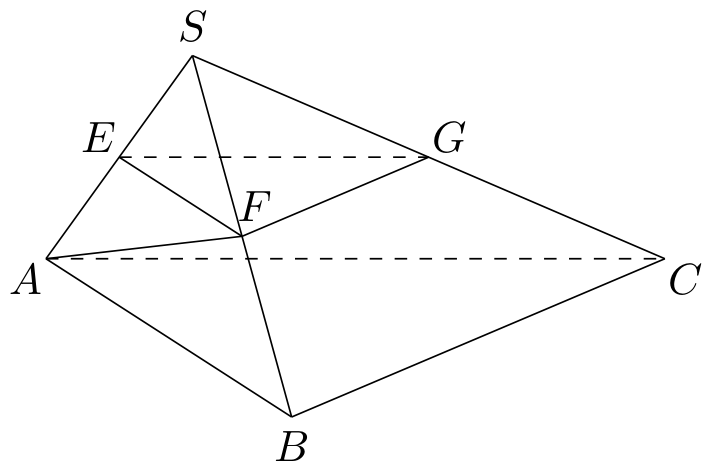
\includegraphics[width=8.3cm]{GaoKao/images/2013/jiangsu/q16_fig1.png}
\end{center}

        \item 如图，在平面直角坐标系 \(xOy\) 中，点 \(A(0,3)\)，直线 \(l:y=2x-4\). 设圆 \(C\) 的半径为 \(1\)，圆心在 \(l\) 上.

\begin{enumerate}
\item 若圆心 \(C\) 也在直线 \(y=x-1\) 上，过点 \(A\) 作圆 \(C\) 的切线，求切线的方程；
\item 若圆 \(C\) 上存在点 \(M\)，使 \(MA=2MO\)，求圆心 \(C\) 的横坐标 \(a\) 的取值范围.
\end{enumerate}

\begin{center}
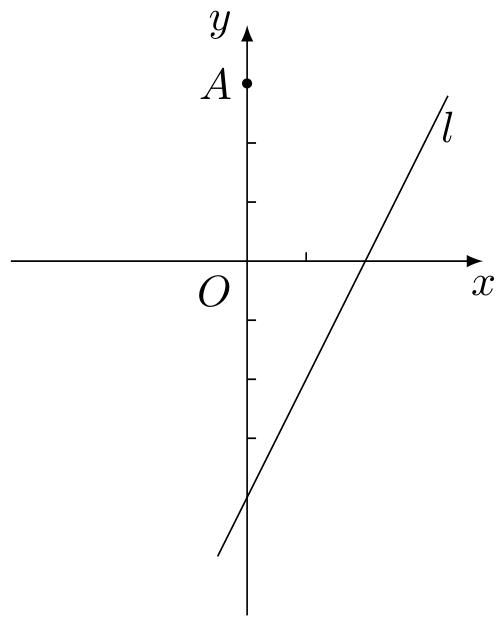
\includegraphics[width=5.9cm]{GaoKao/images/2013/jiangsu/q17_fig1.png}
\end{center}

        \item 如图，游客从某旅游景区的景点 \(A\) 处下山至 \(C\) 处有两种路径. 一种是从 \(A\) 沿直线步行到 \(C\)，另一种是先从 \(A\) 沿索道乘缆车到 \(B\)，然后从 \(B\) 沿直线步行到 \(C\). 现有甲，乙两位游客从 \(A\) 处下山，甲沿 \(AC\) 匀速步行，速度为 \(50\mathrm{~m/min}\). 在甲出发 \(2\mathrm{~min}\) 后，乙从 \(A\) 乘缆车到 \(B\)，在 \(B\) 处停留 \(1\mathrm{~min}\) 后，再从 \(B\) 匀速步行到 \(C\). 假设缆车匀速直线运动的速度为 \(130\mathrm{~m/min}\)，山路 \(AC\) 长为 \(1260\mathrm{~m}\)，经测量，\(\cos A=\frac{12}{13}\)，\(\cos C=\frac{3}{5}\).

\begin{enumerate}
\item 求索道 \(AB\) 的长；
\item 问乙出发多少分钟后，乙在缆车上与甲的距离最短？
\item 为使两位游客在 \(C\) 处互相等待的时间不超过 \(3\mathrm{~min}\)，乙步行的速度应控制在什么范围内？
\end{enumerate}

\begin{center}
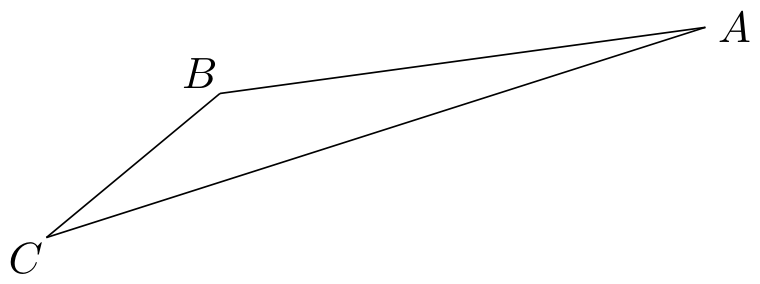
\includegraphics[width=9.4cm]{GaoKao/images/2013/jiangsu/q18_fig1.png}
\end{center}

        \item 设 \(\{a_n\}\) 是首项为 \(a\)，公差为 \(d\) 的等差数列（\(d\ne 0\)），\(S_n\) 是其前 \(n\) 项和. 记 \(b_n=\frac{nS_n}{n^2+c}\)，\(n\in\mathbb{N}^*\)，其中 \(c\) 为实数.

\begin{enumerate}
\item 若 \(c=0\)，且 \(b_1\)，\(b_2\)，\(b_4\) 成等比数列，证明：\(S_{nk}=n^2S_k\)（\(k\)，\(n\in\mathbb{N}^*\)）；
\item 若 \(\{b_n\}\) 是等差数列，证明：\(c=0\).
\end{enumerate}

        \item 设函数 \(f(x)=\ln x-ax\)，\(g(x)={\mathrm{e}}^x-ax\)，其中 \(a\) 为实数.

\begin{enumerate}
\item 若 \(f(x)\) 在 \((1,+\infty)\) 上是单调减函数，且 \(g(x)\) 在 \((1,+\infty)\) 上有最小值，求 \(a\) 的取值范围；
\item 若 \(g(x)\) 在 \((-1,+\infty)\) 上是单调增函数，试求 \(f(x)\) 的零点个数，并证明你的结论.
\end{enumerate}

    \end{enumerate}

\end{description}

\begin{description}

    \item[三、附加题]

    \begin{enumerate}[leftmargin=5pt]

      \addtocounter{enumi}{+20}

        \item [A]
如图，\(AB\) 和 \(BC\) 分别与圆 \(O\) 相切于点 \(D\)，\(C\)，\(AC\) 经过圆心 \(O\)，且 \(BC=2OC\). 求证：\(AC=2AD\).

\begin{center}
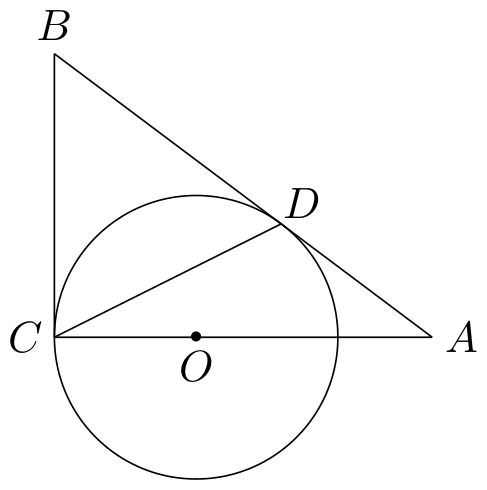
\includegraphics[width=5.7cm]{GaoKao/images/2013/jiangsu/q21_fig1.png}
\end{center}

        \item [B]
已知矩阵 \(A=\begin{bmatrix}-1&0\\0&2\end{bmatrix}\)，\(B=\begin{bmatrix}1&2\\0&6\end{bmatrix}\)，求矩阵 \(A^{-1}B\).

        \item [C]
在平面直角坐标系 \(xOy\) 中，直线 \(l\) 的参数方程为 \(x=t+1\)，\(y=2t\)（\(t\) 为参数），曲线 \(C\) 的参数方程为 \(x=2\tan^2\theta\)，\(y=2\tan\theta\)（\(\theta\) 为参数）. 试求直线 \(l\) 和曲线 \(C\) 的普通方程，并求出它们的公共点的坐标.

        \item [D]
已知 \(a\geqslant b>0\)，求证：\(2a^3-b^3\geqslant 2ab^2-a^2b\).

        \item 如图，在直三棱柱 \(A_1B_1C_1-ABC\) 中，\(AB\perp AC\)，\(AB=AC=2\)，\(A_1A=4\)，点 \(D\) 是 \(BC\) 的中点.

\begin{enumerate}
\item 求异面直线 \(A_1B\) 与 \(C_1D\) 所成角的余弦值；
\item 求平面 \(ADC_1\) 与平面 \(ABA_1\) 所成二面角的正弦值.
\end{enumerate}

\begin{center}
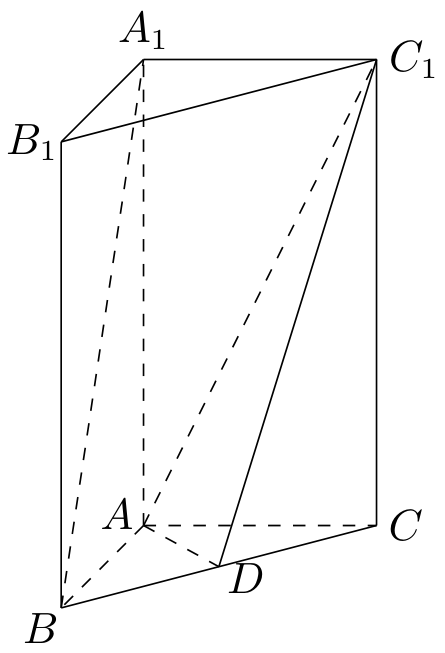
\includegraphics[width=4.4cm]{GaoKao/images/2013/jiangsu/q22_fig1.png}
\end{center}

        \item 设数列 \(\{a_n\}\)：\(1\)，\(-2\)，\(-2\)，\(3\)，\(3\)，\(3\)，\(-4\)，\(-4\)，\(-4\)，\(-4\)，\(\cdots\)，\(\underbrace{(-1)^{k-1}k,\cdots,(-1)^{k-1}k}_{k\text{ 个}}\)，\(\cdots\). 即当 \(\frac{(k-1)k}{2}<n\leqslant \frac{k(k+1)}{2}\)（\(k\in\mathbb{N}^*\)）时，\(a_n=(-1)^{k-1}k\). 记 \(S_n=a_1+a_2+\cdots+a_n\)（\(n\in\mathbb{N}^*\)）. 对于 \(\ell\in\mathbb{N}^*\)，定义集合 \(P_{\ell}=\{n\mid 1\leqslant n\leqslant \ell,\ S_n\text{ 是 }a_n\text{ 的整数倍}\}\).

\begin{enumerate}
\item 求集合 \(P_{11}\) 中元素的个数；
\item 求集合 \(P_{2000}\) 中元素的个数.
\end{enumerate}

    \end{enumerate}

\end{description}


\subsection{2013年江西卷（理）}\label{gk:2013年江西卷（理）}

\begin{description}

    \item[一、选择题]

    \begin{enumerate}[leftmargin=5pt]

        \item 已知集合 \(M = \{1, 2, z\i\}\)，\(\i\) 为虚数单位，\(N = \{3, 4\}\)，\(M \cap N = \{4\}\)，则复数 \(z\) 等于（\quad）

        {\centering\begin{tabular*}{\linewidth}{@{}@{\extracolsep{\fill}}llll@{}}
          \text{A. }\(-2\i\)  &  \text{B. }\(2\i\)  &  \text{C. }\(-4\i\)  &  \text{D. }\(4\i\)
        \end{tabular*}\par}

        \item 函数 \( y = \sqrt{x} \ln (1 - x) \) 的定义域为（\quad）

        {\centering\begin{tabular*}{\linewidth}{@{}@{\extracolsep{\fill}}llll@{}}
          \text{A. }\((0,1)\)  &  \text{B. }\([0,1)\)  &  \text{C. }\((0,1]\)  &  \text{D. }\([0,1]\)
        \end{tabular*}\par}

        \item 等比数列 \(x\)，\(3x + 3\)，\(6x + 6\)，\(\cdots\) 的第四项等于（\quad）

        {\centering\begin{tabular*}{\linewidth}{@{}@{\extracolsep{\fill}}llll@{}}
          \text{A. }\(-24\)  &  \text{B. }0  &  \text{C. }12  &  \text{D. }24
        \end{tabular*}\par}

        \item 总体由编号为 01，02，…，19，20 的 20 个个体组成. 利用下面的随机数表选取 5 个个体，选取方法从随机数表第 1 行的第 5 列和第 6 列数字开始，由左到右依次选取两个数字，则选出来的第 5 个个体的编号为（\quad）

7816 6572 0802 6314 0702 4369 9728 0198 3204 9234 4935 8200 3623 4869 6938 7481

        {\centering\begin{tabular*}{\linewidth}{@{}@{\extracolsep{\fill}}llll@{}}
          \text{A. }08  &  \text{B. }07  &  \text{C. }02  &  \text{D. }01
        \end{tabular*}\par}

        \item \(\left(x^{2} - \frac{2}{x^{3}}\right)^{5}\) 展开式中的常数项为（\quad）

        {\centering\begin{tabular*}{\linewidth}{@{}@{\extracolsep{\fill}}llll@{}}
          \text{A. }80  &  \text{B. }\(-80\)  &  \text{C. }40  &  \text{D. }\(-40\)
        \end{tabular*}\par}

        \item 若 \(S_{1} = \int_{1}^{3} x^{2} \mathrm{d}x\)，\(S_{2} = \int_{1}^{2} \frac{1}{x} \mathrm{d}x\)，\(S_{3} = \int_{1}^{2} {\mathrm{e}}^{x} \mathrm{d}x\)，则 \(S_{1}\)，\(S_{2}\)，\(S_{3}\) 的大小关系为（\quad）

        {\centering\begin{tabular*}{\linewidth}{@{}@{\extracolsep{\fill}}llll@{}}
          \text{A. }\(S_{1} < S_{2} < S_{3}\)  &  \text{B. }\(S_{2} < S_{1} < S_{3}\)  &  \text{C. }\(S_{2} < S_{3} < S_{1}\)  &  \text{D. }\(S_{3} < S_{2} < S_{1}\)
        \end{tabular*}\par}

        \item 阅读如图所示程序框图，如果输出 \(i = 5\)，那么在空白矩形框中应填入的语句为（\quad）

\begin{center}
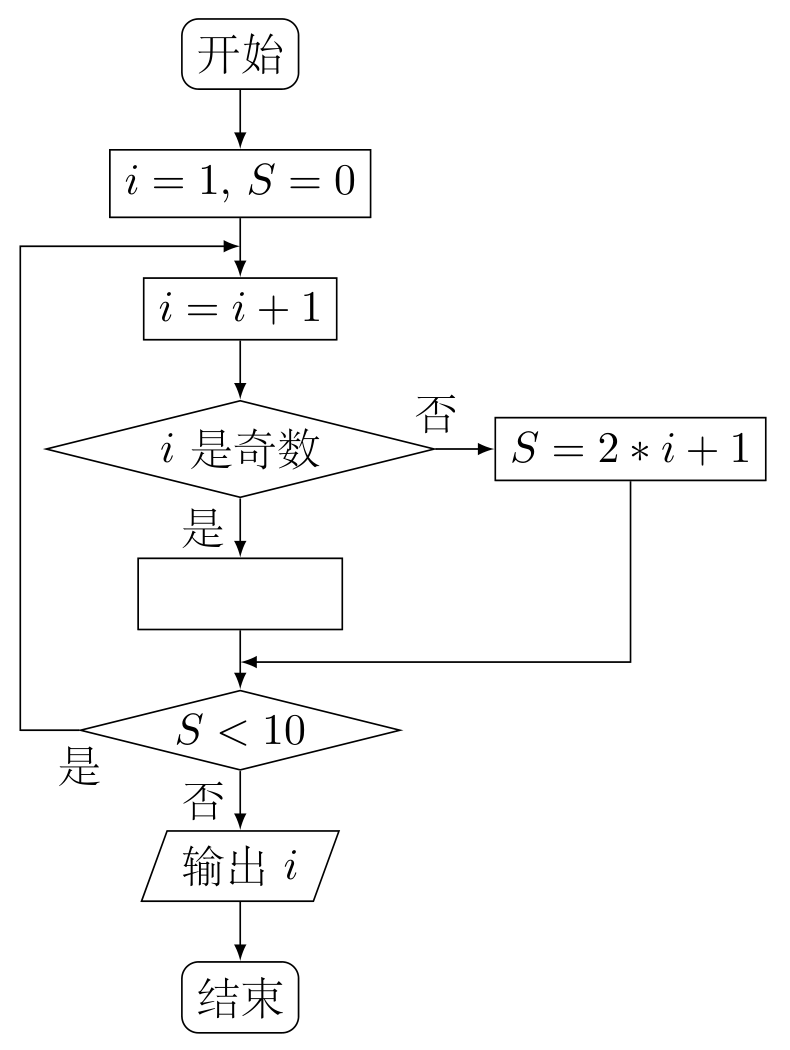
\includegraphics[width=5.8cm]{GaoKao/images/2013/jiangxi_science/q7_fig1.png}
\end{center}

        {\centering\begin{tabular*}{\linewidth}{@{}@{\extracolsep{\fill}}llll@{}}
          \text{A. }\(S = 2 * i - 2\)  &  \text{B. }\(S = 2 * i - 1\)  &  \text{C. }\(S = 2 * i\)  &  \text{D. }\(S = 2 * i + 4\)
        \end{tabular*}\par}

        \item 如图，正方体的底面与正四面体的底面在同一平面 \(\alpha\) 上，且 \(AB \parallel CD\)，正方体的六个面所在的平面与直线 \(CE\)，\(EF\) 相交的平面个数分别记为 \(m\)，\(n\)，那么 \(m + n =\)（\quad）

\begin{center}
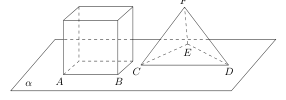
\includegraphics[width=8.9cm]{GaoKao/images/2013/jiangxi_science/q8_fig1.png}
\end{center}

        {\centering\begin{tabular*}{\linewidth}{@{}@{\extracolsep{\fill}}llll@{}}
          \text{A. }8  &  \text{B. }9  &  \text{C. }10  &  \text{D. }11
        \end{tabular*}\par}

        \item 过点 \((\sqrt{2}, 0)\) 引直线 \(l\) 与曲线 \(y = \sqrt{1 - x^{2}}\) 相交于 \(A\)，\(B\) 两点，\(O\) 为坐标原点，当 \(\triangle AOB\) 的面积取最大值时，直线 \(l\) 的斜率等于（\quad）

        {\centering\begin{tabular*}{\linewidth}{@{}@{\extracolsep{\fill}}llll@{}}
          \text{A. }\(\frac{\sqrt{3}}{3}\)  &  \text{B. }\(-\frac{\sqrt{3}}{3}\)  &  \text{C. }\(\pm \frac{\sqrt{3}}{3}\)  &  \text{D. }\(-\sqrt{3}\)
        \end{tabular*}\par}

        \item 如图，半径为 1 的半圆 \(O\) 与等边三角形 \(ABC\) 夹在两平行线 \(l_{1}\)，\(l_{2}\) 之间，\(l \parallel l_{1}\)，\(l\) 与半圆相交于 \(F\)，\(G\) 两点，与三角形 \(ABC\) 两边相交于 \(E\)，\(D\) 两点. 设弧 \(FG\) 的长为 \(x\)（\(0 < x < \pi\)），\(y = EB + BC + CD\)，若 \(l\) 从 \(l_{1}\) 平行移动到 \(l_{2}\)，则函数 \(y = f(x)\) 的图象大致是（\quad）

\begin{center}
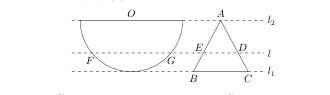
\includegraphics[width=8.0cm]{GaoKao/images/2013/jiangxi_science/q9_fig1.png}
\end{center}

        {\centering\begin{tabular*}{\linewidth}{@{}@{\extracolsep{\fill}}cccc@{}}
          \text{A. }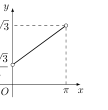
\includegraphics[width=0.15\paperwidth]{GaoKao/images/2013/jiangxi_science/q10_opt_a.png}  &  \text{B. }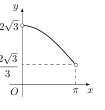
\includegraphics[width=0.15\paperwidth]{GaoKao/images/2013/jiangxi_science/q10_opt_b.png}  &  \text{C. }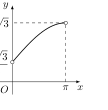
\includegraphics[width=0.15\paperwidth]{GaoKao/images/2013/jiangxi_science/q10_opt_c.png}  &  \text{D. }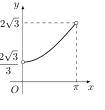
\includegraphics[width=0.15\paperwidth]{GaoKao/images/2013/jiangxi_science/q10_opt_d.png}
        \end{tabular*}\par}

    \end{enumerate}

\end{description}

\begin{description}

    \item[二、填空题]

    \begin{enumerate}[leftmargin=5pt]

      \addtocounter{enumi}{+10}

        \item 函数 \(y = \sin 2x + 2\sqrt{3}\sin^{2}x\) 的最小正周期 \(T\) 为\rule[-0.3ex]{3em}{0.4pt}.

        \item \(\bm{e}_{1}\)，\(\bm{e}_{2}\) 为单位向量，且 \(\bm{e}_{1}\)，\(\bm{e}_{2}\) 的夹角为 \(\frac{\pi}{3}\)，若 \(\bm{a} = \bm{e}_{1} + 3\bm{e}_{2}\)，\(\bm{b} = 2\bm{e}_{1}\)，则向量 \(\bm{a}\) 在 \(\bm{b}\) 方向上的射影为\rule[-0.3ex]{3em}{0.4pt}.

        \item 设函数 \(f(x)\) 在 \((0, +\infty)\) 内可导，且 \(f({\mathrm{e}}^x) = x + {\mathrm{e}}^x\)，则 \(f'(1) =\)\rule[-0.3ex]{3em}{0.4pt}.

        \item 抛物线 \(x^{2} = 2py\)（\(p > 0\)）的焦点为 \(F\)，其准线与双曲线 \(\frac{x^{2}}{3} - \frac{y^{2}}{3} = 1\) 相交于 \(A\)，\(B\) 两点，若 \(\triangle ABF\) 为等边三角形，则 \(p =\)\rule[-0.3ex]{3em}{0.4pt}.

        \item 设曲线 \(C\) 的参数方程为 \(\begin{cases}
x = t,\\
y = t^2
\end{cases}\)（\(t\) 为参数），若以直角坐标系的原点为极点，\(x\) 轴的正半轴为极轴建立极坐标系，则曲线 \(C\) 的极坐标方程为\rule[-0.3ex]{3em}{0.4pt}.

        \item 在实数范围内，不等式 \(||x - 2| - 1| \leqslant 1\) 的解集为\rule[-0.3ex]{3em}{0.4pt}.

    \end{enumerate}

\end{description}

\begin{description}

    \item[三、解答题]

    \begin{enumerate}[leftmargin=5pt]

      \addtocounter{enumi}{+16}

        \item 在 \(\triangle ABC\) 中，角 \(A\)，\(B\)，\(C\) 所对的边分别为 \(a\)，\(b\)，\(c\). 已知 \(\cos C + (\cos A - \sqrt{3}\sin A)\cos B = 0\).

\begin{enumerate}
\item 求角 \(B\) 的大小；
\item 若 \(a + c = 1\)，求 \(b\) 的取值范围.
\end{enumerate}

        \item 正项数列 \(\{a_{n}\}\) 的前 \(n\) 项和 \(S_{n}\) 满足 \(S_{n}^{2} - (n^{2} + n - 1)S_{n} - (n^{2} + n) = 0\).

\begin{enumerate}
\item 求数列 \(\{a_{n}\}\) 的通项公式；
\item 令 \(b_{n} = \frac{n + 1}{(n + 2)^2 a_{n}^{2}}\)，数列 \(\{b_{n}\}\) 的前 \(n\) 项和为 \(T_{n}\). 证明：对于任意 \(n \in \mathbb{N}^{*}\)，都有 \(T_{n} < \frac{5}{64}\).
\end{enumerate}

        \item 小波以游戏方式决定是参加学校合唱团还是参加学校排球队，游戏规则为：以 \(O\) 为起点，再从 \(A_{1}\)，\(A_{2}\)，\(A_{3}\)，\(A_{4}\)，\(A_{5}\)，\(A_{6}\)，\(A_{7}\)，\(A_{8}\)（如图）这 8 个点中任取两点，分别为终点得到两个向量，记这两个向量的数量积为 \(X\). 若 \(X = 0\) 就参加学校合唱团，否则就参加学校排球队.

\begin{enumerate}
\item 求小波参加学校合唱团的概率；
\item 求 \(X\) 的分布列和数学期望.
\end{enumerate}

\begin{center}
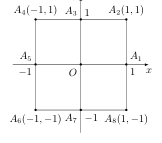
\includegraphics[width=4.4cm]{GaoKao/images/2013/jiangxi_science/q19_fig1.png}
\end{center}

        \item 如图，四棱锥 \(P - ABCD\) 中，\(PA \perp\) 平面 \(ABCD\)，\(E\) 为 \(BD\) 的中点，\(G\) 为 \(PD\) 的中点，\(\triangle DAB \cong \triangle DCB\)，\(EA = EB = AB = 1\)，\(PA = \frac{3}{2}\)，连接 \(CE\) 并延长交 \(AD\) 于 \(F\).

\begin{enumerate}
\item 求证：\(AD \perp\) 平面 \(CFG\)；
\item 求平面 \(BCP\) 与平面 \(DCP\) 的夹角的余弦值.
\end{enumerate}

\begin{center}
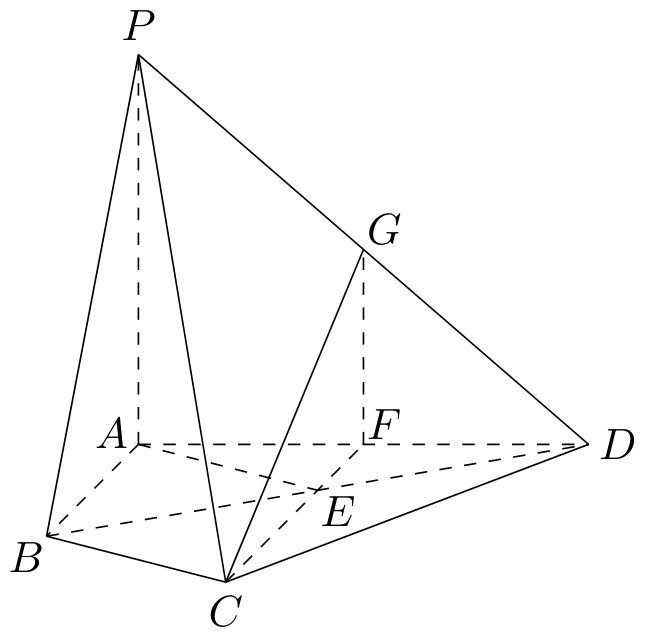
\includegraphics[width=8.0cm]{GaoKao/images/2013/jiangxi_science/q20_fig1.png}
\end{center}

        \item 如图，椭圆 \(C: \frac{x^2}{a^2} + \frac{y^2}{b^2} = 1\)（\(a > b > 0\)）经过点 \(P\left(1, \frac{3}{2}\right)\)，离心率 \(e = \frac{1}{2}\)，直线 \(l\) 的方程为 \(x = 4\).

\begin{enumerate}
\item 求椭圆 \(C\) 的方程；
\item \(AB\) 是经过右焦点 \(F\) 的任一弦（不经过点 \(P\)），设直线 \(AB\) 与直线 \(l\) 相交于点 \(M\)，记 \(PA\)，\(PB\)，\(PM\) 的斜率分别为 \(k_{1}\)，\(k_{2}\)，\(k_{3}\). 问：是否存在常数 \(\lambda\)，使得 \(k_{1} + k_{2} = \lambda k_{3}\)？若存在，求 \(\lambda\) 的值；若不存在，请说明理由.
\end{enumerate}

\begin{center}
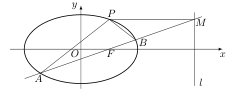
\includegraphics[width=9.3cm]{GaoKao/images/2013/jiangxi_science/q21_fig1.png}
\end{center}

        \item 已知函数 \(f(x) = a\left(1 - 2\left|x - \frac{1}{2}\right|\right)\)，\(a\) 为常数且 \(a > 0\).

\begin{enumerate}
\item 证明：函数 \(f(x)\) 的图象关于直线 \(x = \frac{1}{2}\) 对称；
\item 若 \(x_0\) 满足 \(f(f(x_0)) = x_0\)，且 \(f(x_0) \neq x_0\)，则称 \(x_0\) 为函数 \(f(x)\) 的二阶周期点. 如果 \(f(x)\) 有两个二阶周期点 \(x_1\)，\(x_2\)，试确定 \(a\) 的取值范围；
\item 对于第 2 问中的 \(x_1\)，\(x_2\) 和 \(a\)，设 \(x_3\) 为函数 \(f(f(x))\) 的最大值点，\(A(x_1, f(f(x_1)))\)，\(B(x_2, f(f(x_2)))\)，\(C(x_3, 0)\)，记 \(\triangle ABC\) 的面积为 \(S(a)\)，讨论 \(S(a)\) 的单调性.
\end{enumerate}

    \end{enumerate}

\end{description}


\subsection{2013年江西卷（文）}\label{gk:2013年江西卷（文）}

\begin{description}

    \item[一、选择题]

    \begin{enumerate}[leftmargin=5pt]

        \item 复数 \(z = \i(-2 - \i)\)（\(\i\) 为虚数单位）在复平面内所对应的点在（\quad）

        {\centering\begin{tabular*}{\linewidth}{@{}@{\extracolsep{\fill}}llll@{}}
          \text{A. }第一象限  &  \text{B. }第二象限  &  \text{C. }第三象限  &  \text{D. }第四象限
        \end{tabular*}\par}

        \item 若集合 \(A = \{x \in \mathbb{R} \mid ax^2 + ax + 1 = 0\}\) 中只有一个元素，则 \(a =\)（\quad）

        {\centering\begin{tabular*}{\linewidth}{@{}@{\extracolsep{\fill}}llll@{}}
          \text{A. }4  &  \text{B. }2  &  \text{C. }0  &  \text{D. }0 或 4
        \end{tabular*}\par}

        \item 若 \(\sin \frac{\alpha}{2} = \frac{\sqrt{3}}{3}\)，则 \(\cos \alpha =\)（\quad）

        {\centering\begin{tabular*}{\linewidth}{@{}@{\extracolsep{\fill}}llll@{}}
          \text{A. }\(-\frac{2}{3}\)  &  \text{B. }\(-\frac{1}{3}\)  &  \text{C. }\( \frac{1}{3} \)  &  \text{D. }\( \frac{2}{3} \)
        \end{tabular*}\par}

        \item 集合 \(A = \{2, 3\}\)，\(B = \{1, 2, 3\}\)，从 \(A\)，\(B\) 中各任意取一个数，则这两数之和等于 4 的概率是（\quad）

        {\centering\begin{tabular*}{\linewidth}{@{}@{\extracolsep{\fill}}llll@{}}
          \text{A. }\( \frac{2}{3} \)  &  \text{B. }\( \frac{1}{2} \)  &  \text{C. }\( \frac{1}{3} \)  &  \text{D. }\( \frac{1}{6} \)
        \end{tabular*}\par}

        \item 总体由编号为 \(01\)，\(02\)，…，\(19\)，\(20\) 的 20 个个体组成. 利用下面的随机数表选取 5 个个体，选取方法从随机数表第 \(1\) 行的第 \(5\) 列和第 \(6\) 列数字开始由左到右依次选取两个数字，则选出来的第 \(5\) 个个体的编号为（\quad）

7816 6572 0802 6314 0702 4369 9728 0198 3204 9234 4935 8200 3623 4869 6938 7481

        {\centering\begin{tabular*}{\linewidth}{@{}@{\extracolsep{\fill}}llll@{}}
          \text{A. }08  &  \text{B. }07  &  \text{C. }02  &  \text{D. }01
        \end{tabular*}\par}

        \item 下列选项中，使不等式 \(x < \frac{1}{x} < x^2\) 成立的 \(x\) 的取值范围是（\quad）

        {\centering\begin{tabular*}{\linewidth}{@{}@{\extracolsep{\fill}}llll@{}}
          \text{A. }\((- \infty, -1)\)  &  \text{B. }\((-1,0)\)  &  \text{C. }\((0,1)\)  &  \text{D. }\((1, +\infty)\)
        \end{tabular*}\par}

        \item 阅读如图所示程序框图，如果输出 \(i = 4\)，那么在空白的判断框中应填入的条件是（\quad）

\begin{center}
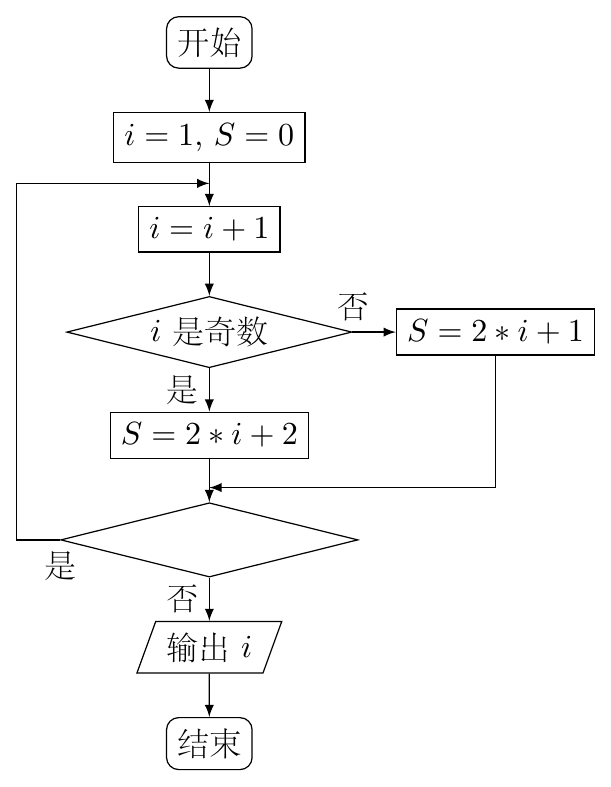
\includegraphics[width=0.34\linewidth]{GaoKao/images/2013/jiangxi_liberal/q7_fig1.png}
\end{center}

        {\centering\begin{tabular*}{\linewidth}{@{}@{\extracolsep{\fill}}llll@{}}
          \text{A. }\(S < 8\)  &  \text{B. }\(S < 9\)  &  \text{C. }\(S < 10\)  &  \text{D. }\(S < 11\)
        \end{tabular*}\par}

        \item 一几何体的三视图如图所示，则该几何体的体积为


\begin{center}
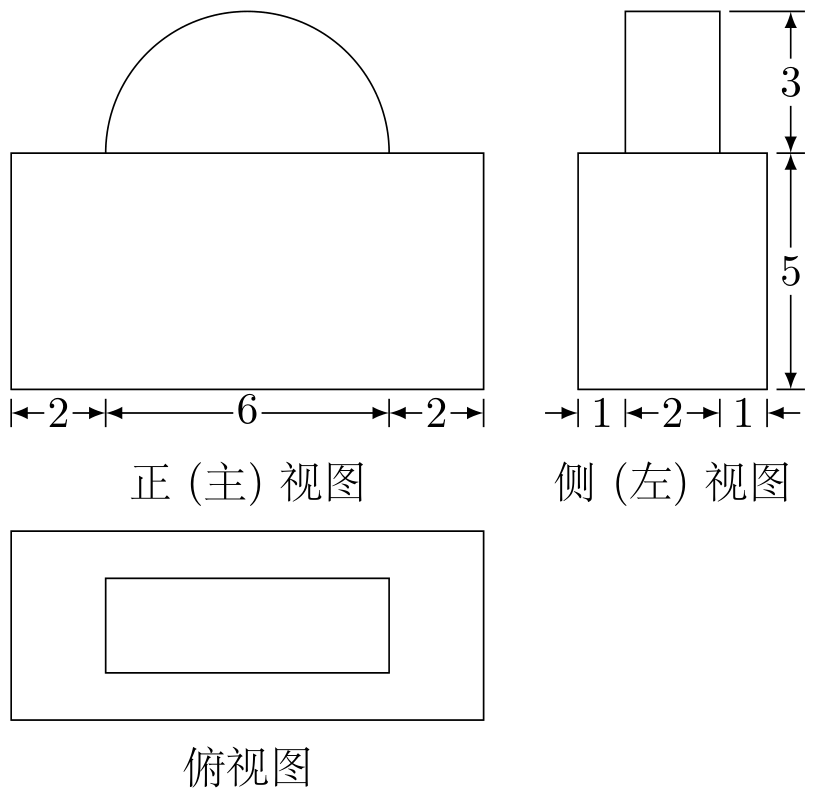
\includegraphics[width=8.0cm]{GaoKao/images/2013/jiangxi_liberal/q8_fig1.png}
\end{center}

（\quad）

        {\centering\begin{tabular*}{\linewidth}{@{}@{\extracolsep{\fill}}llll@{}}
          \text{A. }\(200 + 9\pi\)  &  \text{B. }\(200 + 18\pi\)  &  \text{C. }\(140 + 9\pi\)  &  \text{D. }\(140 + 18\pi\)
        \end{tabular*}\par}

        \item 已知点 \(A(2,0)\)，抛物线 \(C: x^2 = 4y\) 的焦点为 \(F\)，射线 \(FA\) 与抛物线 \(C\) 相交于点 \(M\)，与其准线相交于点 \(N\)，则 \(|FM|: |MN| =\)（\quad）

        {\centering\begin{tabular*}{\linewidth}{@{}@{\extracolsep{\fill}}llll@{}}
          \text{A. }\(2:\sqrt{5}\)  &  \text{B. }\(1:2\)  &  \text{C. }\( 1 : \sqrt{5} \)  &  \text{D. }\(1:3\)
        \end{tabular*}\par}

        \item 如图，已知 \(l_{1} \perp l_{2}\)，圆心在 \(l_{1}\) 上，半径为 \(1 \mathrm{~m}\) 的圆 \(O\) 在 \(t = 0\) 时与 \(l_{2}\) 相切于点 \(A\)，圆 \(O\) 沿 \(l_{1}\) 以 \(1 \mathrm{~m} / \mathrm{s}\) 的速度匀速向上移动，圆被直线 \(l_{2}\) 所截上方圆弧长记为 \(x\)，令 \(y = \cos x\)，则 \(y\) 与时间 \(t\)（\(0 \leqslant t \leqslant 1\)，单位：\(\mathrm{s}\)）的函数 \(y = f(t)\) 的图象大致为（\quad）

\begin{center}
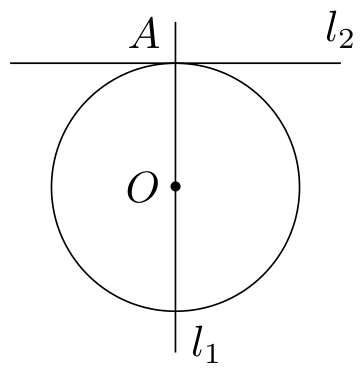
\includegraphics[width=3.6cm]{GaoKao/images/2013/jiangxi_liberal/q10_fig1.png}
\end{center}

        {\centering\begin{tabular*}{\linewidth}{@{}@{\extracolsep{\fill}}cccc@{}}
          \text{A. }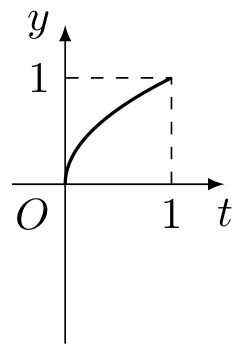
\includegraphics[width=0.15\paperwidth]{GaoKao/images/2013/jiangxi_liberal/q10_opt_a.png}  &  \text{B. }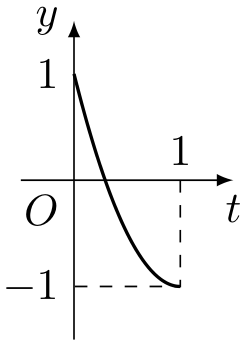
\includegraphics[width=0.15\paperwidth]{GaoKao/images/2013/jiangxi_liberal/q10_opt_b.png}  &  \text{C. }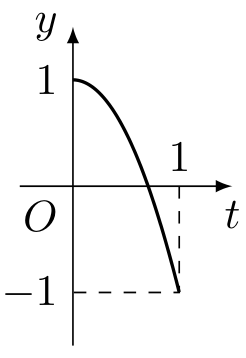
\includegraphics[width=0.15\paperwidth]{GaoKao/images/2013/jiangxi_liberal/q10_opt_c.png}  &  \text{D. }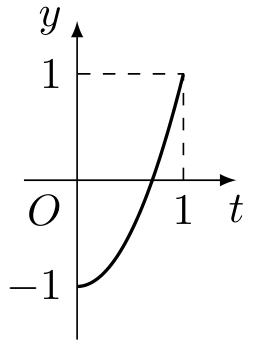
\includegraphics[width=0.15\paperwidth]{GaoKao/images/2013/jiangxi_liberal/q10_opt_d.png}
        \end{tabular*}\par}

    \end{enumerate}

\end{description}

\begin{description}

    \item[二、填空题]

    \begin{enumerate}[leftmargin=5pt]

      \addtocounter{enumi}{+10}

        \item 若曲线 \(y = x^{\alpha} + 1\)（\(\alpha \in \mathbb{R}\)）在点 \((1,2)\) 处的切线经过坐标原点，则 \( \alpha = \)\rule[-0.3ex]{3em}{0.4pt}.

        \item 某住宅小区计划植树不少于 100 棵，若第一天植 2 棵，以后每天植树的棵数是前一天的 2 倍，则需要的最少天数 \(n\)（\(n \in \mathbb{N}^{*}\)）等于\rule[-0.3ex]{3em}{0.4pt}.

        \item 设 \( f(x) = \sqrt{3} \sin 3x + \cos 3x \)，若对任意实数 \( x \) 都有 \( |f(x)| \leqslant a \)，则实数 \( a \) 的取值范围是\rule[-0.3ex]{3em}{0.4pt}.

        \item 若圆 \(C\) 经过坐标原点和点 \((4,0)\)，且与直线 \(y = 1\) 相切，则圆 \(C\) 的方程是\rule[-0.3ex]{3em}{0.4pt}.

        \item 如图，正方体的底面与正四面体的底面在同一平面 \(\alpha\) 上，且 \(AB \parallel CD\)，则直线 \(EF\) 与正方体的六个面所在的平面相交的平面个数为\rule[-0.3ex]{3em}{0.4pt}.
\begin{center}
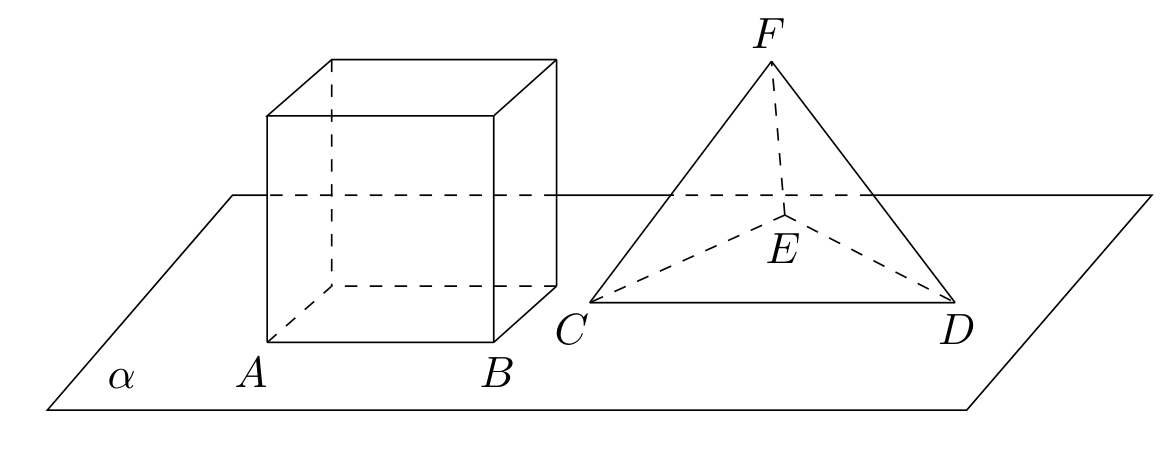
\includegraphics[width=11.0cm]{GaoKao/images/2013/jiangxi_liberal/q15_fig1.png}
\end{center}

    \end{enumerate}

\end{description}

\begin{description}

    \item[三、解答题]

    \begin{enumerate}[leftmargin=5pt]

      \addtocounter{enumi}{+15}

        \item 正项数列 \(\{a_{n}\}\) 满足： \(a_{n}^{2} - (2n - 1)a_{n} - 2n = 0\).
\begin{enumerate}
\item 求数列 \( \{a_{n}\} \) 的通项公式；
\item 令 \( b_{n} = \frac{1}{(n + 1)a_{n}} \)，求数列 \( \{b_{n}\} \) 的前 \( n \) 项和 \( T_{n} \).
\end{enumerate}

        \item 在 \(\triangle ABC\) 中，角 \(A\)，\(B\)，\(C\) 的对边分别为 \(a\)，\(b\)，\(c\). 已知 \(\sin A \sin B + \sin B \sin C + \cos 2B = 1\).
\begin{enumerate}
\item 求证： \(a\)，\(b\)，\(c\) 成等差数列；
\item 若 \(C = \frac{2\pi}{3}\)，求 \(\frac{a}{b}\) 的值.
\end{enumerate}

        \item 小波以游戏方式决定是去打球，唱歌还是去下棋，游戏规则为：以 \(O\) 为起点，再从 \(A_{1}\)，\(A_{2}\)，\(A_{3}\)，\(A_{4}\)，\(A_{5}\)，\(A_{6}\)（如图）这 \(6\) 个点中任取两点分别为终点得到两个向量，记这两个向量的数量积为 \(X\)，若 \(X > 0\) 就去打球，若 \(X = 0\) 就去唱歌，若 \(X < 0\) 就去下棋.
\begin{enumerate}
\item 写出数量积 \(X\) 的所有可能取值；
\item 分别求小波去下棋的概率和不去唱歌的概率.
\end{enumerate}
\begin{center}
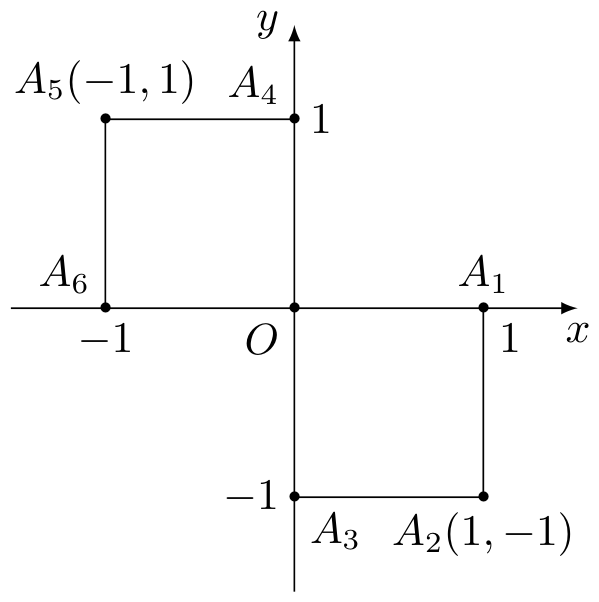
\includegraphics[width=4.2cm]{GaoKao/images/2013/jiangxi_liberal/q18_fig1.png}
\end{center}

        \item 如图，直四棱柱 \(ABCD - A_{1}B_{1}C_{1}D_{1}\) 中，\(AB \parallel CD\)，\(AD \perp AB\)，\(AB = 2\)，\(AD = \sqrt{2}\)，\(AA_{1} = 3\)，\(E\) 为 \(CD\) 上一点，\(DE = 1\)，\(EC = 3\).
\begin{enumerate}
\item 证明： \(BE \perp\) 平面 \(BB_{1}C_{1}C\)；
\item 求点 \(B_{1}\) 到平面 \(EA_{1}C_{1}\) 的距离.
\end{enumerate}
\begin{center}
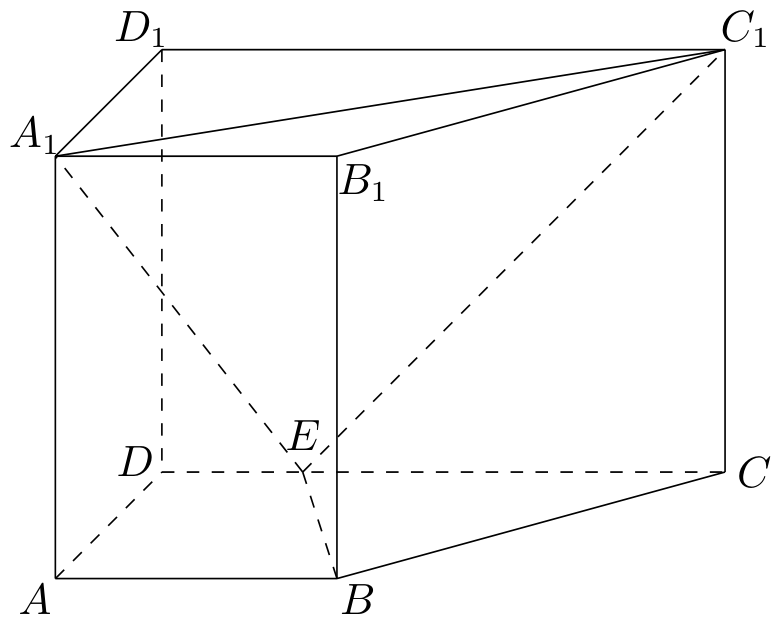
\includegraphics[width=7.9cm]{GaoKao/images/2013/jiangxi_liberal/q19_fig1.png}
\end{center}

        \item 椭圆 \(C\)：\(\frac{x^2}{a^2} + \frac{y^2}{b^2} = 1\)（\(a > b > 0\)）的离心率 \(e = \frac{\sqrt{3}}{2}\)，\(a + b = 3\).
\begin{enumerate}
\item 求椭圆 \(C\) 的方程；
\item 如图所示，\(A\)，\(B\)，\(D\) 是椭圆 \(C\) 的顶点，\(P\) 是椭圆 \(C\) 上除顶点外的任意一点，直线 \(DP\) 交 \(x\) 轴于点 \(N\)，直线 \(AD\) 交 \(BP\) 于点 \(M\)，设 \(BP\) 的斜率为 \(k\)，\(MN\) 的斜率为 \(m\)，证明：\(2m-k\) 为定值.
\end{enumerate}
\begin{center}
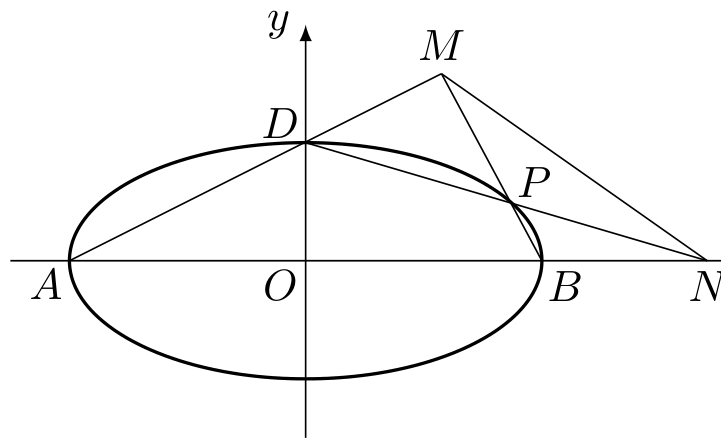
\includegraphics[width=9.0cm]{GaoKao/images/2013/jiangxi_liberal/q20_fig1.png}
\end{center}

        \item 设函数 \( f(x) = \begin{cases}
\frac{1}{a} x, & 0 \leqslant x \leqslant a,\\
\frac{1}{1 - a} (1 - x), & a < x \leqslant 1,
\end{cases} \) \( a \) 为常数且 \( a \in (0,1) \).
\begin{enumerate}
\item 当 \(a = \frac{1}{2}\) 时，求 \(f\left(f\left(\frac{1}{3}\right)\right)\)；
\item 若 \(x_0\) 满足 \(f(f(x_0)) = x_0\)，但 \(f(x_0) \neq x_0\)，则称 \(x_0\) 为 \(f(x)\) 的二阶周期点，证明：函数 \(f(x)\) 有且仅有两个二阶周期点，并求出二阶周期点 \(x_1\)，\(x_2\)；
\item 对于（2）中的 \(x_{1}\)，\(x_{2}\)，设 \(A\left(x_{1}, f(f(x_{1}))\right)\)，\(B\left(x_{2}, f(f(x_{2}))\right)\)，\(C\left(a^{2}, 0\right)\)，记 \(\triangle ABC\) 的面积为 \(S(a)\)，求 \(S(a)\) 在区间 \(\left[\frac{1}{3}, \frac{1}{2}\right]\) 上的最大值和最小值.
\end{enumerate}

    \end{enumerate}

\end{description}


\subsection{2013年辽宁卷（理）}\label{gk:2013年辽宁卷（理）}

\begin{description}

    \item[一、选择题]

    \begin{enumerate}[leftmargin=5pt]

        \item 复数 \(z = \frac{1}{\i - 1}\) 的模为（\quad）

        {\centering\begin{tabular*}{\linewidth}{@{}@{\extracolsep{\fill}}llll@{}}
          \text{A. }\(\frac{1}{2}\)  &  \text{B. }\(\frac{\sqrt{2}}{2}\)  &  \text{C. }\(\sqrt{2}\)  &  \text{D. }\(2\)
        \end{tabular*}\par}

        \item 已知集合 \(A = \{x \mid 0 < \log_4 x < 1\}\)，\(B = \{x \mid x \leqslant 2\}\)，则 \(A \cap B =\)（\quad）

        {\centering\begin{tabular*}{\linewidth}{@{}@{\extracolsep{\fill}}llll@{}}
          \text{A. }\((0,1)\)  &  \text{B. }\((0,2]\)  &  \text{C. }\((1,2)\)  &  \text{D. }\((1,2]\)
        \end{tabular*}\par}

        \item 已知点 \(A(1,3)\)，\(B(4,-1)\)，则与向量 \(\overrightarrow{AB}\) 同方向的单位向量为（\quad）

        {\centering\begin{tabular*}{\linewidth}{@{}@{\extracolsep{\fill}}llll@{}}
          \text{A. }\(\left(\frac{3}{5}, -\frac{4}{5}\right)\)  &  \text{B. }\(\left(\frac{4}{5}, -\frac{3}{5}\right)\)  &  \text{C. }\(\left(-\frac{3}{5}, \frac{4}{5}\right)\)  &  \text{D. }\(\left(-\frac{4}{5}, \frac{3}{5}\right)\)
        \end{tabular*}\par}

        \item 下面是关于公差 \(d > 0\) 的等差数列 \(\{a_n\}\) 的四个命题：

\begin{enumerate}
\item 数列 \(\{a_n\}\) 是递增数列
\item 数列 \(\{na_n\}\) 是递增数列
\item 数列 \(\left\{\frac{a_n}{n}\right\}\) 是递增数列
\item 数列 \(\{a_n + 3nd\}\) 是递增数列
\end{enumerate}

其中的真命题为（\quad）

        {\centering\begin{tabular*}{\linewidth}{@{}@{\extracolsep{\fill}}llll@{}}
          \text{A. }\(p_1\)，\(p_2\)  &  \text{B. }\(p_3\)，\(p_4\)  &  \text{C. }\(p_2\)，\(p_3\)  &  \text{D. }\(p_1\)，\(p_4\)
        \end{tabular*}\par}

        \item 某班的全体学生参加英语测试，成绩的频率分布直方图如图，数据的分组依次为：\([20,40)\)，\([40,60)\)，\([60,80)\)，\([80,100]\). 若低于 \(60\) 分的人数是 \(15\)，则该班的学生人数是（\quad）

\begin{center}
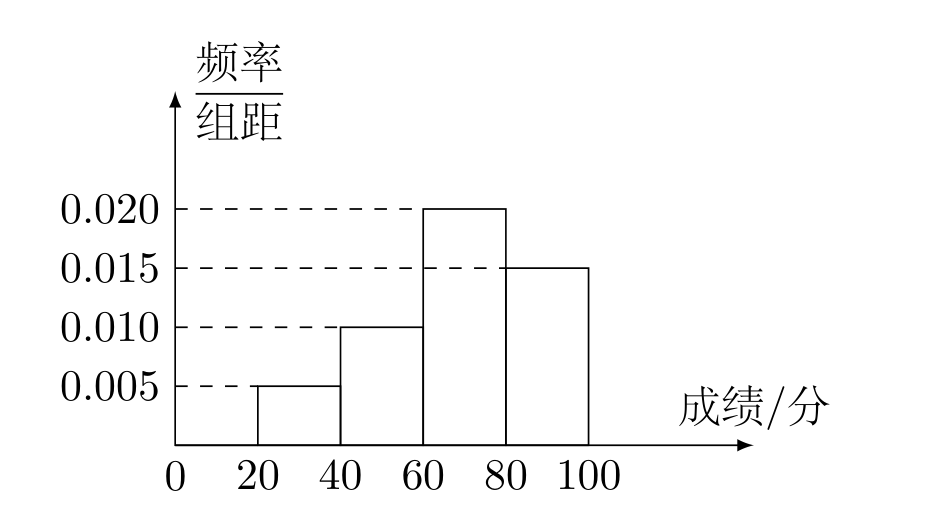
\includegraphics[width=0.46\linewidth]{GaoKao/images/2013/liaoning_science/q5_fig1.png}
\end{center}

        {\centering\begin{tabular*}{\linewidth}{@{}@{\extracolsep{\fill}}llll@{}}
          \text{A. }\(45\)  &  \text{B. }\(50\)  &  \text{C. }\(55\)  &  \text{D. }\(60\)
        \end{tabular*}\par}

        \item 在 \(\triangle ABC\) 中，内角 \(A\)，\(B\)，\(C\) 所对的边分别为 \(a\)，\(b\)，\(c\)，若 \(a \sin B \cos C + c \sin B \cos A = \frac{1}{2} b\)，且 \(a > b\)，则 \(\angle B =\)（\quad）

        {\centering\begin{tabular*}{\linewidth}{@{}@{\extracolsep{\fill}}llll@{}}
          \text{A. }\(\frac{\pi}{6}\)  &  \text{B. }\(\frac{\pi}{3}\)  &  \text{C. }\(\frac{2\pi}{3}\)  &  \text{D. }\(\frac{5\pi}{6}\)
        \end{tabular*}\par}

        \item 使 \(\left(3x + \frac{1}{x\sqrt{x}}\right)^n\)（\(n \in \mathbf{N}_{+}\)）的展开式中含有常数项的最小的 \(n\) 为（\quad）

        {\centering\begin{tabular*}{\linewidth}{@{}@{\extracolsep{\fill}}llll@{}}
          \text{A. }\(4\)  &  \text{B. }\(5\)  &  \text{C. }\(6\)  &  \text{D. }\(7\)
        \end{tabular*}\par}

        \item 执行如图所示的程序框图，若输入 \(n = 10\)，则输出 \(S =\)（\quad）

\begin{center}
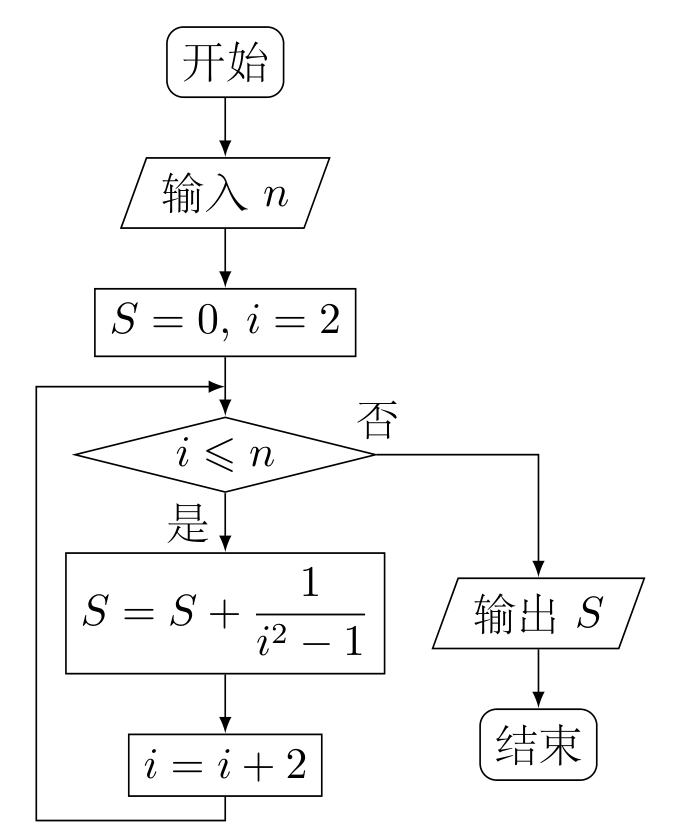
\includegraphics[width=0.26\linewidth]{GaoKao/images/2013/liaoning_science/q8_fig1.png}
\end{center}

        {\centering\begin{tabular*}{\linewidth}{@{}@{\extracolsep{\fill}}llll@{}}
          \text{A. }\(\frac{5}{11}\)  &  \text{B. }\(\frac{10}{11}\)  &  \text{C. }\(\frac{36}{55}\)  &  \text{D. }\(\frac{72}{55}\)
        \end{tabular*}\par}

        \item 已知点 \(O(0,0)\)，\(A(0,b)\)，\(B(a,a^{3})\). 若 \(\triangle OAB\) 为直角三角形，则必有（\quad）

        {\centering\begin{tabular*}{\linewidth}{@{}@{\extracolsep{\fill}}llll@{}}
          \text{A. }\(b = a^{3}\)  &  \text{B. }\(b = a^{3} + \frac{1}{a}\)  &  \text{C. }\(\left(b - a^{3}\right)\left(b - a^{3} - \frac{1}{a}\right) = 0\)  &  \text{D. }\(\left|b - a^3\right| + \left|b - a^3 - \frac{1}{a}\right| = 0\)
        \end{tabular*}\par}

        \item 已知直三棱柱 \(ABC-A_1B_1C_1\) 的 \(6\) 个顶点都在球 \(O\) 的球面上. 若 \(AB = 3\)，\(AC = 4\)，\(AB \perp AC\)，\(AA_1 = 12\)，则球 \(O\) 的半径为（\quad）

        {\centering\begin{tabular*}{\linewidth}{@{}@{\extracolsep{\fill}}llll@{}}
          \text{A. }\(\frac{3\sqrt{17}}{2}\)  &  \text{B. }\(2\sqrt{10}\)  &  \text{C. }\(\frac{13}{2}\)  &  \text{D. }\(3\sqrt{10}\)
        \end{tabular*}\par}

        \item 已知函数 \(f(x) = x^2 - 2(a + 2)x + a^2\)，\(g(x) = -x^2 + 2(a - 2)x - a^2 + 8\)，设 \(H_1(x) = \max\{f(x), g(x)\}\)，\(H_2(x) = \min\{f(x), g(x)\}\)（\(\max\{p, q\}\) 表示 \(p\)，\(q\) 中的较大值，\(\min\{p, q\}\) 表示 \(p\)，\(q\) 中的较小值）. 记 \(H_1(x)\) 的最小值为 \(A\)，\(H_2(x)\) 的最大值为 \(B\)，则 \(A - B =\)（\quad）

        {\centering\begin{tabular*}{\linewidth}{@{}@{\extracolsep{\fill}}llll@{}}
          \text{A. }\(16\)  &  \text{B. }\(-16\)  &  \text{C. }\(a^2 - 2a - 16\)  &  \text{D. }\(a^2 + 2a - 16\)
        \end{tabular*}\par}

        \item 设函数 \( f(x) \) 满足 \(x^{2}f'(x) + 2xf(x) = \frac{{\mathrm{e}}^{x}}{x}\)，\(f(2) = \frac{{\mathrm{e}}^{2}}{8}\)，则 \( x > 0 \) 时，\( f(x) \)（\quad）

        {\centering\begin{tabular*}{\linewidth}{@{}@{\extracolsep{\fill}}llll@{}}
          \text{A. }有极大值，无极小值  &  \text{B. }有极小值，无极大值  &  \text{C. }既有极大值又有极小值  &  \text{D. }既无极大值也无极小值
        \end{tabular*}\par}

    \end{enumerate}

\end{description}

\begin{description}

    \item[二、填空题]

    \begin{enumerate}[leftmargin=5pt]

      \addtocounter{enumi}{+12}

        \item 某几何体的三视图如图所示，则该几何体的体积是\rule[-0.3ex]{3em}{0.4pt}.

\begin{center}
\includegraphics[width=3.0cm]{GaoKao/images/2013/liaoning_science/q13_fig1.png}
\end{center}

        \item 已知等比数列 \(\{a_n\}\) 是递增数列，\(S_n\) 是 \(\{a_n\}\) 的前 \(n\) 项和，若 \(a_1\)，\(a_3\) 是方程 \(x^2 - 5x + 4 = 0\) 的两个根，则 \(S_6 =\)\rule[-0.3ex]{3em}{0.4pt}.

        \item 已知椭圆 \(C:\frac{x^2}{a^2} + \frac{y^2}{b^2} = 1\)（\(a > b > 0\)）的左焦点为 \(F\)，\(C\) 与过原点的直线相交于 \(A\)，\(B\) 两点，连接 \(AF\)，\(BF\)，若 \(|AB| = 10\)，\(|AF| = 6\)，\(\cos \angle ABF = \frac{4}{5}\)，则椭圆 \(C\) 的离心率 \(e =\)\rule[-0.3ex]{3em}{0.4pt}.

        \item 为了考察某校各班参加课外书法小组的人数，从全校随机抽取 \(5\) 个班级，把每个班级参加该小组的人数作为样本数据. 已知样本平均数为 \(7\)，样本方差为 \(4\)，且样本数据互不相同，则样本数据中的最大值为\rule[-0.3ex]{3em}{0.4pt}.

    \end{enumerate}

\end{description}

\begin{description}

    \item[三、解答题]

    \begin{enumerate}[leftmargin=5pt]

      \addtocounter{enumi}{+16}

        \item 设向量 \(\bm{a} = (\sqrt{3}\sin x, \sin x)\)，\(\bm{b} = (\cos x, \sin x)\)，\(x \in \left[0, \frac{\pi}{2}\right]\).

\begin{enumerate}
\item 若 \(\left|\bm{a}\right| = \left|\bm{b}\right|\)，求 \(x\) 的值；
\item 设函数 \(f(x) = \bm{a} \cdot \bm{b}\)，求 \(f(x)\) 的最大值.
\end{enumerate}

        \item 如图，\(AB\) 是圆的直径，\(PA\) 垂直圆所在的平面，\(C\) 是圆上的点.

\begin{enumerate}
\item 求证：平面 \(PAC \perp PBC\)；
\item 若 \(AB = 2\)，\(AC = 1\)，\(PA = 1\)，求二面角 \(C - PB - A\) 的余弦值.
\end{enumerate}

\begin{center}
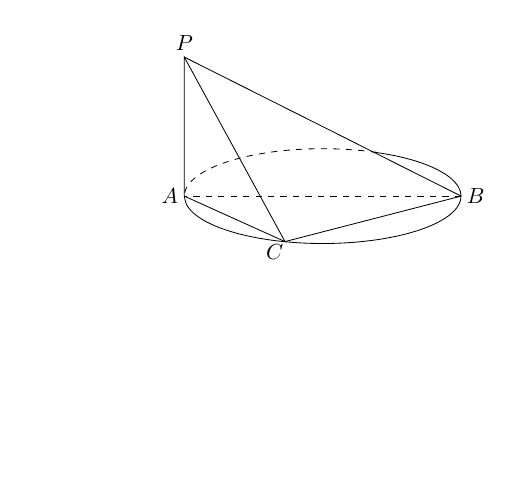
\includegraphics[width=8.0cm]{GaoKao/images/2013/liaoning_science/q18_fig1.png}
\end{center}

        \item 现有 \(10\) 道题，其中 \(6\) 道甲类题，\(4\) 道乙类题，张同学从中任取 \(3\) 道题解答.

\begin{enumerate}
\item 求张同学至少取到 \(1\) 道乙类题的概率；
\item 已知所取的 \(3\) 道题中有 \(2\) 道甲类题，\(1\) 道乙类题. 设张同学答对每道甲类题的概率都是 \(\frac{3}{5}\)，答对每道乙类题的概率都是 \(\frac{4}{5}\)，且各题答对与否相互独立. 用 \(X\) 表示张同学答对题的个数，求 \(X\) 的分布列和数学期望.
\end{enumerate}

        \item 如图，抛物线 \(C_1:x^2 = 4y\)，\(C_2:x^2 = -2py\)（\(p > 0\)）. 点 \(M(x_0, y_0)\) 在抛物线 \(C_2\) 上，过 \(M\) 作 \(C_1\) 的切线，切点为 \(A\)，\(B\)（\(M\) 为原点 \(O\) 时，\(A\)，\(B\) 重合于 \(O\)）. 当 \(x_0 = 1 - \sqrt{2}\) 时，切线 \(MA\) 的斜率为 \(-\frac{1}{2}\).

\begin{enumerate}
\item 求 \(p\) 的值；
\item 当 \(M\) 在 \(C_2\) 上运动时，求线段 \(AB\) 中点 \(N\) 的轨迹方程（\(A\)，\(B\) 重合于 \(O\) 时，中点为 \(O\)）.
\end{enumerate}

\begin{center}
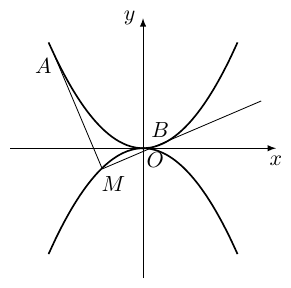
\includegraphics[width=7.2cm]{GaoKao/images/2013/liaoning_science/q20_fig1.png}
\end{center}

        \item 已知函数 \(f(x) = (1 + x){\mathrm{e}}^{-2x}\)，\(g(x) = ax + \frac{x^3}{2} + 1 + 2x\cos x\)，当 \(x \in [0,1]\) 时，

\begin{enumerate}
\item 求证：\(1 - x \leqslant f(x) \leqslant \frac{1}{1 + x}\)；
\item 若 \(f(x) \geqslant g(x)\) 恒成立，求实数 \(a\) 的取值范围.
\end{enumerate}

    \end{enumerate}

\end{description}

\begin{description}

    \item[四、选考题]

    \begin{enumerate}[leftmargin=5pt]

      \addtocounter{enumi}{+21}

        \item 如图，\(AB\) 为 \(\odot O\) 直径，直线 \(CD\) 与 \(\odot O\) 相切于 \(E\)，\(AD\) 垂直 \(CD\) 于 \(D\)，\(BC\) 垂直 \(CD\) 于 \(C\)，\(EF\) 垂直 \(AB\) 于 \(F\)，连接 \(AE\)，\(BE\). 证明：

\begin{enumerate}
\item \(\angle FEB = \angle CEB\)；
\item \(EF^2 = AD \cdot BC\).
\end{enumerate}

\begin{center}
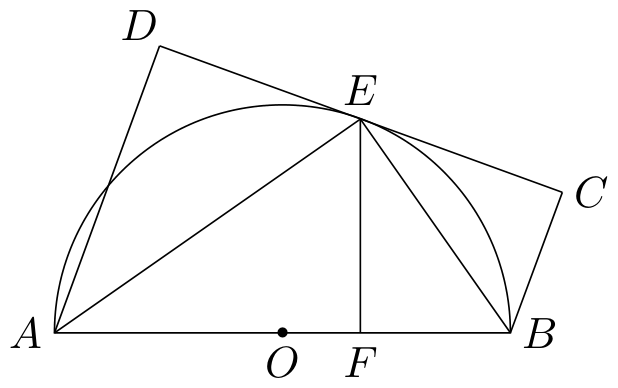
\includegraphics[width=7.7cm]{GaoKao/images/2013/liaoning_science/q22_fig1.png}
\end{center}

        \item \textbf{【选修4-4：坐标系与参数方程】}

在直角坐标系 \(xOy\) 中，以 \(O\) 为极点，\(x\) 轴正半轴为极轴建立极坐标系. 圆 \(C_1\)，直线 \(C_2\) 的极坐标方程分别为 \(\rho = 4\sin \theta\)，\(\rho \cos \left(\theta - \frac{\pi}{4}\right) = 2\sqrt{2}\).

\begin{enumerate}
\item 求 \(C_1\) 与 \(C_2\) 交点的极坐标；
\item 设 \(P\) 为 \(C_1\) 的圆心，\(Q\) 为 \(C_1\) 与 \(C_2\) 交点连线的中点，已知直线 \(PQ\) 的参数方程为 \(\begin{cases}
x = t^3 + a,\\
y = \frac{b}{2}t^3 + 1,
\end{cases}\)（\(t \in \mathbb{R}\) 为参数），求 \(a\)，\(b\) 的值.
\end{enumerate}

        \item \textbf{【选修4-5：不等式选讲】}

已知函数 \(f(x) = |x - a|\)，其中 \(a > 1\).

\begin{enumerate}
\item 当 \(a = 2\) 时，求不等式 \(f(x) \geqslant 4 - |x - 4|\) 的解集；
\item 已知关于 \(x\) 的不等式 \(\left|f(2x + a) - 2f(x)\right| \leqslant 2\) 的解集为 \(\{x \mid 1 \leqslant x \leqslant 2\}\)，求 \(a\) 的值.
\end{enumerate}

    \end{enumerate}

\end{description}


\subsection{2013年辽宁卷（文）}\label{gk:2013年辽宁卷（文）}

\begin{description}

    \item[一、选择题]

    \begin{enumerate}[leftmargin=5pt]

        \item 已知集合 \(A = \{0, 1, 2, 3, 4\}\)，\(B = \{x \mid |x| < 2\}\)，则 \(A \cap B =\)（\quad）

        {\centering\begin{tabular*}{\linewidth}{@{}@{\extracolsep{\fill}}llll@{}}
          \text{A. }\( \{0\} \)  &  \text{B. }\(\{0,1\}\)  &  \text{C. }\(\{0,2\}\)  &  \text{D. }\(\{0,1,2\}\)
        \end{tabular*}\par}

        \item 复数的 \(z = \frac{1}{\i - 1}\) 模为（\quad）

        {\centering\begin{tabular*}{\linewidth}{@{}@{\extracolsep{\fill}}llll@{}}
          \text{A. }\(\frac{1}{2}\)  &  \text{B. }\(\frac{\sqrt{2}}{2}\)  &  \text{C. }\(\sqrt{2}\)  &  \text{D. }\(2\)
        \end{tabular*}\par}

        \item 已知点 \(A(1,3)\)，\(B(4,-1)\)，则与向量 \(\overrightarrow{AB}\) 同方向的单位向量为（\quad）

        {\centering\begin{tabular*}{\linewidth}{@{}@{\extracolsep{\fill}}llll@{}}
          \text{A. }\(\left(\frac{3}{5}, -\frac{4}{5}\right)\)  &  \text{B. }\( \left(\frac{4}{5},-\frac{3}{5}\right) \)  &  \text{C. }\( \left(\frac{3}{5},\frac{4}{5}\right) \)  &  \text{D. }\(\left(-\frac{3}{5}, \frac{4}{5}\right)\)
        \end{tabular*}\par}

        \item 下面是关于公差 \(d > 0\) 的等差数列 \(\{a_{n}\}\) 的四个命题：

\begin{enumerate}
\item \(p_{1}\)：数列 \(\{a_{n}\}\) 是递增数列；
\item \(p_{2}\)：数列 \(\{na_{n}\}\) 是递增数列；
\item \(p_{3}\)：数列 \(\left\{\frac{a_{n}}{n}\right\}\) 是递增数列；
\item \(p_{4}\)：数列 \(\{a_{n}+3nd\}\) 是递增数列.
\end{enumerate}

其中的真命题为（\quad）

        {\centering\begin{tabular*}{\linewidth}{@{}@{\extracolsep{\fill}}llll@{}}
          \text{A. }\(p_1\)，\(p_2\)  &  \text{B. }\(p_3\)，\(p_4\)  &  \text{C. }\(p_2\)，\(p_3\)  &  \text{D. }\(p_1\)，\(p_4\)
        \end{tabular*}\par}

        \item 某班的全体学生参加英语测试，成绩的频率分布直方图如图，数据的分组依次为：\([20,40)\)，\([40,60)\)，\([60,80)\)，\([80,100]\). 若低于 \(60\) 分的人数是 \(15\)，则该班的学生人数是（\quad）

\begin{center}
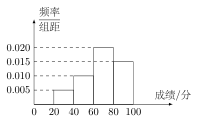
\includegraphics[width=0.42\linewidth]{GaoKao/images/2013/liaoning_liberal/q5_fig1.png}
\end{center}

        {\centering\begin{tabular*}{\linewidth}{@{}@{\extracolsep{\fill}}llll@{}}
          \text{A. }\(45\)  &  \text{B. }\(50\)  &  \text{C. }\(55\)  &  \text{D. }\(60\)
        \end{tabular*}\par}

        \item 在 \(\triangle ABC\) 中，内角 \(A\)，\(B\)，\(C\) 所对的边分别为 \(a\)，\(b\)，\(c\)，若 \(a \sin B \cos C + c \sin B \cos A = \frac{1}{2} b\)，且 \(a > b\)，则 \(\angle B =\)（\quad）

        {\centering\begin{tabular*}{\linewidth}{@{}@{\extracolsep{\fill}}llll@{}}
          \text{A. }\(\frac{\pi}{6}\)  &  \text{B. }\(\frac{\pi}{3}\)  &  \text{C. }\(\frac{2\pi}{3}\)  &  \text{D. }\(\frac{5\pi}{6}\)
        \end{tabular*}\par}

        \item 已知函数 \( f(x) = \ln (\sqrt{1 + 9x^2} - 3x) + 1 \)，则 \( f(\lg 2) + f\left(\lg \frac{1}{2}\right) = \)（\quad）

        {\centering\begin{tabular*}{\linewidth}{@{}@{\extracolsep{\fill}}llll@{}}
          \text{A. }\(-1\)  &  \text{B. }\(0\)  &  \text{C. }\(1\)  &  \text{D. }\(2\)
        \end{tabular*}\par}

        \item 执行如图所示的程序框图，若输入 \(n = 8\)，则输出 \(S =\)（\quad）

\begin{center}
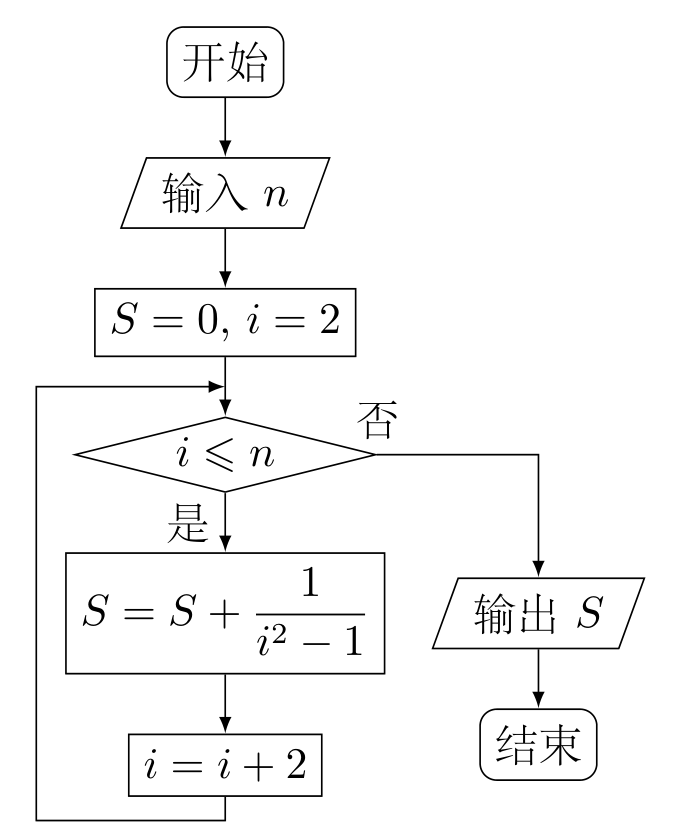
\includegraphics[width=0.24\linewidth]{GaoKao/images/2013/liaoning_liberal/q8_fig1.png}
\end{center}

        {\centering\begin{tabular*}{\linewidth}{@{}@{\extracolsep{\fill}}llll@{}}
          \text{A. }\(\frac{4}{9}\)  &  \text{B. }\(\frac{6}{7}\)  &  \text{C. }\(\frac{8}{9}\)  &  \text{D. }\(\frac{10}{11}\)
        \end{tabular*}\par}

        \item 已知点 \(O(0,0)\)，\(A(0,b)\)，\(B(a,a^3)\). 若 \(\triangle OAB\) 为直角三角形，则必有（\quad）

        {\centering\begin{tabular*}{\linewidth}{@{}@{\extracolsep{\fill}}llll@{}}
          \text{A. }\(b = a^3\)  &  \text{B. }\(b = a^3 + \frac{1}{a}\)  &  \text{C. }\((b - a^3)\left(b - a^3 - \frac{1}{a}\right) = 0\)  &  \text{D. }\( |b - a^3| + \left|b - a^3 - \frac{1}{a}\right| = 0 \)
        \end{tabular*}\par}

        \item 已知直三棱柱 \(ABC-A_{1}B_{1}C_{1}\) 的 \(6\) 个顶点都在球 \(O\) 的球面上. 若 \(AB = 3\)，\(AC = 4\)，\(AB \perp AC\)，\(AA_{1} = 12\)，则球 \(O\) 的半径为（\quad）

        {\centering\begin{tabular*}{\linewidth}{@{}@{\extracolsep{\fill}}llll@{}}
          \text{A. }\(\frac{3\sqrt{17}}{2}\)  &  \text{B. }\(2\sqrt{10}\)  &  \text{C. }\(\frac{13}{2}\)  &  \text{D. }\(3\sqrt{10}\)
        \end{tabular*}\par}

        \item 已知椭圆 \(C:\frac{x^2}{a^2} + \frac{y^2}{b^2} = 1\)（\(a > b > 0\)）的左焦点为 \(F\)，\(C\) 与过原点的直线相交于 \(A\)，\(B\) 两点，连接 \(AF\)，\(BF\)，若 \(|AB| = 10\)，\(|BF| = 8\)，\(\cos \angle ABF = \frac{4}{5}\)，则 \(C\) 的离心率为（\quad）

        {\centering\begin{tabular*}{\linewidth}{@{}@{\extracolsep{\fill}}llll@{}}
          \text{A. }\(\frac{3}{5}\)  &  \text{B. }\( \frac{5}{7} \)  &  \text{C. }\( \frac{4}{5} \)  &  \text{D. }\( \frac{6}{7} \)
        \end{tabular*}\par}

        \item 已知函数 \( f(x) = x^2 - 2(a + 2)x + a^2 \)，\( g(x) = -x^2 + 2(a - 2)x - a^2 + 8 \)，设 \( H_1(x) = \max \{f(x), g(x)\} \)，\( H_2(x) = \min \{f(x), g(x)\} \)（\(\max \{p, q\}\) 表示 \(p\)，\(q\) 中的较大值，\(\min \{p, q\}\) 表示 \(p\)，\(q\) 中的较小值）. 记 \( H_1(x) \) 的最小值为 \(A\)，\( H_2(x) \) 的最大值为 \(B\)，则 \( A - B = \)（\quad）

        {\centering\begin{tabular*}{\linewidth}{@{}@{\extracolsep{\fill}}llll@{}}
          \text{A. }\(16\)  &  \text{B. }\(-16\)  &  \text{C. }\(a^2 - 2a - 16\)  &  \text{D. }\(a^2 + 2a - 16\)
        \end{tabular*}\par}

    \end{enumerate}

\end{description}

\begin{description}

    \item[二、填空题]

    \begin{enumerate}[leftmargin=5pt]

      \addtocounter{enumi}{+12}

        \item 某几何体的三视图如图所示.

\begin{center}
\includegraphics[width=3.0cm]{GaoKao/images/2013/liaoning_liberal/q13_fig1.png}
\end{center}

则该几何体的体积是\rule[-0.3ex]{3em}{0.4pt}.

        \item 已知等比数列 \(\{a_n\}\) 是递增数列，\(S_n\) 是 \(\{a_n\}\) 的前 \(n\) 项和. 若 \(a_1\)，\(a_3\) 是方程 \(x^2 - 5x + 4 = 0\) 的两个根，则 \(S_6 =\)\rule[-0.3ex]{3em}{0.4pt}.

        \item 已知 \(F\) 为双曲线 \(C:\frac{x^2}{9} - \frac{y^2}{16} = 1\) 的左焦点，\(P\)，\(Q\) 为 \(C\) 上的点. 若 \(PQ\) 的长等于虚轴长的 \(2\) 倍，点 \(A(5,0)\) 在线段 \(PQ\) 上，则 \(\triangle PQF\) 的周长为\rule[-0.3ex]{3em}{0.4pt}.

        \item 为了考察某校各班参加课外书法小组的人数，从全校随机抽取 \(5\) 个班级，把每个班级参加该小组的人数作为样本数据. 已知样本平均数为 \(7\)，样本方差为 \(4\)，且样本数据互不相同，则样本数据中的最大值为\rule[-0.3ex]{3em}{0.4pt}.

    \end{enumerate}

\end{description}

\begin{description}

    \item[三、解答题]

    \begin{enumerate}[leftmargin=5pt]

      \addtocounter{enumi}{+16}

        \item \begin{enumerate}
\item 设向量 \(\bm{a} = (\sqrt{3}\sin x, \sin x)\)，\(\bm{b} = (\cos x, \sin x)\)，\(x \in \left[0, \frac{\pi}{2}\right]\). 若 \(\left|\bm{a}\right| = \left|\bm{b}\right|\)，求 \(x\) 的值；
\item 设函数 \(f(x) = \bm{a} \cdot \bm{b}\)，求 \(f(x)\) 的最大值.
\end{enumerate}

        \item \begin{enumerate}
\item 如图，\(AB\) 是圆的直径，\(PA\) 垂直圆所在的平面，\(C\) 是圆上的点. 求证：\(BC \perp\) 平面 \(PAC\)；
\item 设 \(Q\) 为 \(PA\) 的中点，\(G\) 为 \(\triangle AOC\) 的重心，求证：\(QG\parallel\) 平面 \(PBC\).
\end{enumerate}
\begin{center}
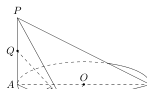
\includegraphics[width=7.1cm]{GaoKao/images/2013/liaoning_liberal/q18_fig1.png}
\end{center}

        \item 现有 \(6\) 道题，其中 \(4\) 道甲类题，\(2\) 道乙类题，张同学从中任取 \(2\) 道题解答. 试求：

\begin{enumerate}
\item 所取的 \(2\) 道题都是甲类题的概率；
\item 所取的 \(2\) 道题不是同一类题的概率.
\end{enumerate}

        \item 如图，抛物线 \(C_{1}:x^{2} = 4y\)，\(C_{2}:x^{2} = -2py\)（\(p > 0\)）. 点 \(M(x_{0}, y_{0})\) 在抛物线 \(C_{2}\) 上，过 \(M\) 作 \(C_{1}\) 的切线，切点为 \(A\)，\(B\)（\(M\) 为原点 \(O\) 时，\(A\)，\(B\) 重合于 \(O\)）. 当 \(x_{0} = 1 - \sqrt{2}\) 时，切线 \(MA\) 的斜率为 \(-\frac{1}{2}\).

\begin{enumerate}
\item 求 \(p\) 的值；
\item 当 \(M\) 在 \(C_{2}\) 上运动时，求线段 \(AB\) 中点 \(N\) 的轨迹方程（\(A\)，\(B\) 重合于 \(O\) 时，中点为 \(O\)）.
\end{enumerate}

\begin{center}
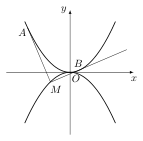
\includegraphics[width=5.8cm]{GaoKao/images/2013/liaoning_liberal/q20_fig1.png}
\end{center}

        \item \begin{enumerate}
\item 证明：当 \(x \in [0,1]\) 时，\(\frac{\sqrt{2}}{2}x \leqslant \sin x \leqslant x\)；
\item 若不等式 \(ax + x^2 + \frac{x^3}{2} + 2(x + 2)\cos x \leqslant 4\) 对 \(x \in [0,1]\) 恒成立，求实数 \(a\) 的取值范围.
\end{enumerate}

    \end{enumerate}

\end{description}

\begin{description}

    \item[四、选考题]

    \begin{enumerate}[leftmargin=5pt]

      \addtocounter{enumi}{+21}

        \item \begin{enumerate}
\item 如图，\(AB\) 为 \(\odot O\) 直径，直线 \(CD\) 与 \(\odot O\) 相切于 \(E\)，\(AD\) 垂直 \(CD\) 于 \(D\)，\(BC\) 垂直 \(CD\) 于 \(C\)，\(EF\) 垂直 \(AB\) 于 \(F\)，连接 \(AE\)，\(BE\). 证明：\(\angle FEB = \angle CEB\)；
\item 证明：\(EF^{2} = AD\cdot BC\).
\end{enumerate}
\begin{center}
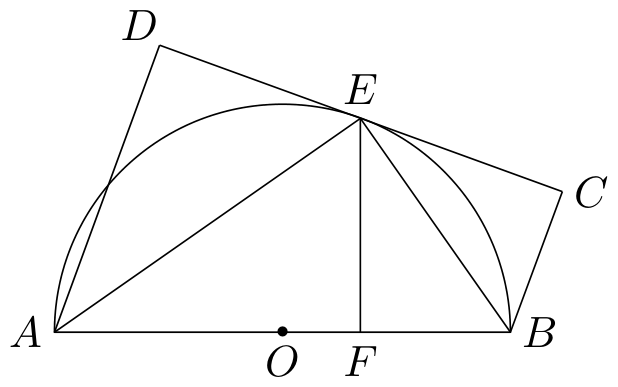
\includegraphics[width=7.7cm]{GaoKao/images/2013/liaoning_liberal/q22_fig1.png}
\end{center}

        \item \textbf{【选修4-4：坐标系与参数方程】}

在直角坐标系 \(xOy\) 中，以 \(O\) 为极点，\(x\) 轴正半轴为极轴建立极坐标系. 圆 \(C_{1}\)，直线 \(C_{2}\) 的极坐标方程分别为 \(\rho = 4\sin \theta\)，\(\rho \cos \left(\theta - \frac{\pi}{4}\right) = 2\sqrt{2}\).

\begin{enumerate}
\item 求 \(C_{1}\) 与 \(C_{2}\) 交点的极坐标；
\item 设 \(P\) 为 \(C_{1}\) 的圆心，\(Q\) 为 \(C_{1}\) 与 \(C_{2}\) 交点连线的中点，已知直线 \(PQ\) 的参数方程为 \(\begin{cases}
x = t^3 + a,\\
y = \frac{b}{2} t^3 + 1,
\end{cases}\)（\(t \in \mathbb{R}\) 为参数），求 \(a\)，\(b\) 的值.
\end{enumerate}

        \item \textbf{【选修4-5：不等式选讲】}

已知函数 \(f(x) = |x - a|\)，其中 \(a > 1\).

\begin{enumerate}
\item 当 \(a = 2\) 时，求不等式 \(f(x) \geqslant 4 - |x - 4|\) 的解集；
\item 已知关于 \(x\) 的不等式 \(\left|f(2x + a) - 2f(x)\right| \leqslant 2\) 的解集为 \(\{x \mid 1 \leqslant x \leqslant 2\}\)，求 \(a\) 的值.
\end{enumerate}

    \end{enumerate}

\end{description}


\subsection{2013年上海卷（理）}\label{gk:2013年上海卷（理）}

\begin{description}

    \item[一、填空题]

    \begin{enumerate}[leftmargin=5pt]

        \item 计算： \(\displaystyle\lim_{n\to\infty}\frac{n+20}{3n+13}=\rule[-0.3ex]{3em}{0.4pt}\)

        \item 设 \(m \in \mathbb{R}\)，\(m^2 + m - 2 + (m^2 - 1)\i\) 是纯虚数，其中 \(\i\) 是虚数单位，则 \(m=\)\rule[-0.3ex]{3em}{0.4pt}.

        \item 若 \(\left|\begin{matrix}x^2 & y^2 \\ -1 & 1\end{matrix}\right| = \left|\begin{matrix}x & x \\ y & -y\end{matrix}\right|\)，则 \(x+y=\)\rule[-0.3ex]{3em}{0.4pt}.

        \item 已知 \(\triangle ABC\) 的内角 \(A\)，\(B\)，\(C\) 所对的边分别为 \(a\)，\(b\)，\(c\). 若 \(3a^2+2ab+3b^2-3c^2=0\)，则角 \(C\) 的大小是\rule[-0.3ex]{3em}{0.4pt}. （结果用反三角函数值表示）

        \item 设常数 \(a \in \mathbb{R}\). 若 \(\left(x^2+\frac{a}{x}\right)^5\) 的二项展开式中 \(x^7\) 项的系数为 \(-10\)，则 \(a=\)\rule[-0.3ex]{3em}{0.4pt}.

        \item 方程 \(\frac{3}{3^x-1}+\frac{1}{3}=3^{x-1}\) 的实数解为\rule[-0.3ex]{3em}{0.4pt}.

        \item 在极坐标系中，曲线 \(\rho=\cos\theta+1\) 与 \(\rho\cos\theta=1\) 的公共点到极点的距离为\rule[-0.3ex]{3em}{0.4pt}.

        \item 盒子中装有编号为 \(1\)，\(2\)，\(3\)，\(4\)，\(5\)，\(6\)，\(7\)，\(8\)，\(9\) 的九个球，从中任意取出两个，则这两个球的编号之积为偶数的概率是\rule[-0.3ex]{3em}{0.4pt}.（结果用最简分数表示）

        \item 设 \(AB\) 是椭圆 \(\Gamma\) 的长轴，点 \(C\) 在 \(\Gamma\) 上，且 \(\angle CBA=\frac{\pi}{4}\)，若 \(AB=4\)，\(BC=\sqrt{2}\)，则 \(\Gamma\) 的两个焦点之间的距离为\rule[-0.3ex]{3em}{0.4pt}.

        \item 设非零常数 \(d\) 是等差数列 \(x_1\)，\(x_2\)，\(x_3\)，\(\cdots\)，\(x_{19}\) 的公差，随机变量 \(\xi\) 等可能地取值 \(x_1\)，\(x_2\)，\(\cdots\)，\(x_{19}\)，则方差 \(D(\xi)=\)\rule[-0.3ex]{3em}{0.4pt}.

        \item 若 \(\cos x\cos y+\sin x\sin y=\frac{1}{2}\)，\(\sin 2x+\sin 2y=\frac{2}{3}\)，则 \(\sin(x+y)=\)\rule[-0.3ex]{3em}{0.4pt}.

        \item 设 \(a\) 为实常数，\(y=f(x)\) 是定义在 \(\mathbb{R}\) 上的奇函数，当 \(x<0\) 时， \(f(x)=9x+\frac{a^2}{x}+7.\)
若 \(f(x)\geqslant a+1\) 对一切 \(x\geqslant 0\) 成立，则 \(a\) 的取值范围为\rule[-0.3ex]{3em}{0.4pt}.

        \item 在 \(xOy\) 平面上，将两个半圆弧 \((x-1)^2+y^2=1\) （\(x\geqslant 1\)）和 \((x-3)^2+y^2=1\)（\(x\geqslant 3\)），两条直线 \(y=1\) 和 \(y=-1\) 围成的封闭图形记为 \(D\)，如图中阴影部分. 记 \(D\) 绕 \(y\) 轴旋转一周而成的几何体为 \(\Omega\)，过 \((0,y)\) （\(|y|\leqslant 1\)）作 \(\Omega\) 的水平截面，所得截面面积为 \(4\pi\sqrt{1-y^2}+8\pi\)，试利用祖暅原理，一个平放的圆柱和一个长方体，得出 \(\Omega\) 的体积为\rule[-0.3ex]{3em}{0.4pt}.
\begin{center}
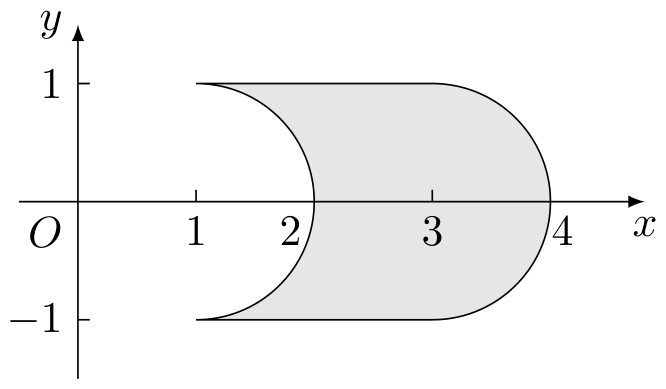
\includegraphics[width=6.6cm]{GaoKao/images/2013/shanghai_science/q13_fig1.png}
\end{center}

        \item 对区间 \(I\) 上有定义的函数 \(g(x)\)，记 \(g(I)=\{y\mid y=g(x),x\in I\}\)，已知定义域为 \([0,3]\) 的函数 \(y=f(x)\) 有反函数 \(y=f^{-1}(x)\)，且 \(f^{-1}([0,1))=[1,2)\)，\(f^{-1}((2,4])=[0,1)\)，若方程 \(f(x)-x=0\) 有解 \(x_0\)，则 \(x_0=\rule[-0.3ex]{3em}{0.4pt}.\)

    \end{enumerate}

\end{description}

\begin{description}

    \item[二、选择题]

    \begin{enumerate}[leftmargin=5pt]

      \addtocounter{enumi}{+14}

        \item 设常数 \(a \in \mathbb{R}\)，集合 \(A=\{x\mid(x-1)(x-a)\geqslant 0\}\)，\(B=\{x\mid x\geqslant a-1\}\). 若 \(A\cup B=\mathbb{R}\)，则 \(a\) 的取值范围为（\quad）

        {\centering\begin{tabular*}{\linewidth}{@{}@{\extracolsep{\fill}}llll@{}}
          \text{A. }\((-\infty,2)\)  &  \text{B. }\((-\infty,2]\)  &  \text{C. }\((2,+\infty)\)  &  \text{D. }\([2,+\infty)\)
        \end{tabular*}\par}

        \item 钱大姐常说“便宜没好货”，她这句话的意思是：“不便宜”是“好货”的（\quad）

        {\centering\begin{tabular*}{\linewidth}{@{}@{\extracolsep{\fill}}llll@{}}
          \text{A. }充分条件  &  \text{B. }必要条件  &  \text{C. }充分必要条件  &  \text{D. }既非充分也非必要条件
        \end{tabular*}\par}

        \item 在数列 \(\{a_n\}\) 中，\(a_n=2^n-1\)，若一个 \(7\) 行 \(12\) 列的矩阵的第 \(i\) 行第 \(j\) 列的元素 \(a_{ij}=a_i\cdot a_j+a_i+a_j\) （\(i=1,2,\cdots,7;\ j=1,2,\cdots,12\)），则该矩阵元素能取到的不同数值的个数为（\quad）

        {\centering\begin{tabular*}{\linewidth}{@{}@{\extracolsep{\fill}}llll@{}}
          \text{A. }18  &  \text{B. }28  &  \text{C. }48  &  \text{D. }63
        \end{tabular*}\par}

        \item 在边长为 \(1\) 的正六边形 \(ABCDEF\) 中，记以 \(A\) 为起点，其余顶点为终点的向量分别为 \(\bm{a}_1\)，\(\bm{a}_2\)，\(\bm{a}_3\)，\(\bm{a}_4\)，\(\bm{a}_5\)；以 \(D\) 为起点，其余顶点为终点的向量分别为 \(\bm{d}_1\)，\(\bm{d}_2\)，\(\bm{d}_3\)，\(\bm{d}_4\)，\(\bm{d}_5\). 若 \(m\)，\(M\) 分别为 \((\bm{a}_i+\bm{a}_j+\bm{a}_k)\cdot(\bm{d}_r+\bm{d}_s+\bm{d}_t)\) 的最小值，最大值，其中 \(\{i,j,k\}\subseteq\{1,2,3,4,5\}\)，\(\{r,s,t\}\subseteq\{1,2,3,4,5\}\)，则 \(m\)，\(M\) 满足（\quad）

        {\centering\begin{tabular*}{\linewidth}{@{}@{\extracolsep{\fill}}llll@{}}
          \text{A. }\(m=0\)，\(M>0\)  &  \text{B. }\(m<0\)，\(M>0\)  &  \text{C. }\(m<0\)，\(M=0\)  &  \text{D. }\(m<0\)，\(M<0\)
        \end{tabular*}\par}

    \end{enumerate}

\end{description}

\begin{description}

    \item[三、解答题]

    \begin{enumerate}[leftmargin=5pt]

      \addtocounter{enumi}{+18}

        \item 如图，在长方体 \(ABCD-A'B'C'D'\) 中，\(AB=2\)，\(AD=1\)，\(AA'=1\)，证明直线 \(BC'\) 平行于平面 \(D'AC\)，并求直线 \(BC'\) 到平面 \(D'AC\) 的距离.
\begin{center}
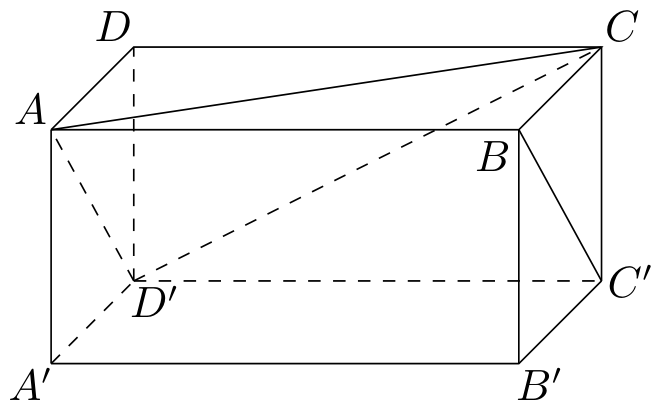
\includegraphics[width=7.5cm]{GaoKao/images/2013/shanghai_science/q19_fig1.png}
\end{center}

        \item 甲厂以 \(x\) 千克/小时的速度运输生产某种产品（生产条件要求 \(1\leqslant x\leqslant 10\)），每一小时可获得利润是 \(100\left(5x+1-\frac{3}{x}\right)\) 元.
\begin{enumerate}
\item 要使生产该产品 \(2\) 小时获得的利润不低于 \(3000\) 元，求 \(x\) 的取值范围；
\item 要使生产 \(900\) 千克该产品获得的利润最大，问：甲厂应该选取何种生产速度？并求最大利润.
\end{enumerate}

        \item 已知函数 \(f(x)=2\sin\omega x\). 其中常数 \(\omega>0\).
\begin{enumerate}
\item 若 \(y=f(x)\) 在 \(\left[-\frac{\pi}{4},\frac{2\pi}{3}\right]\) 上单调递增，求 \(\omega\) 的取值范围；
\item 令 \(\omega=2\)，将函数 \(y=f(x)\) 的图象向左平移 \(\frac{\pi}{6}\) 个单位，再向上平移 \(1\) 个单位，得到函数 \(y=g(x)\) 的图象. 区间 \([a,b]\) （\(a,b\in\mathbb{R}\) 且 \(a<b\)）满足：\(y=g(x)\) 在 \([a,b]\) 上至少含有 \(30\) 个零点. 在所有满足上述条件的 \([a,b]\) 中，求 \(b-a\) 的最小值.
\end{enumerate}

        \item 如图，已知双曲线 \(C_1:\frac{x^2}{2}-y^2=1\)，曲线 \(C_2:|y|=|x|+1\). \(P\) 是平面内一点，若存在过点 \(P\) 的直线与 \(C_1\)，\(C_2\) 都有公共点，则称 \(P\) 为 “\(C_1-C_2\) 型点”.
\begin{enumerate}
\item 在正确证明 \(C_1\) 的左焦点是“\(C_1-C_2\) 型点”时，要使用一条过该焦点的直线，试写出一条这样的直线的方程（不要求验证）；
\item 设直线 \(y=kx\) 与 \(C_2\) 有公共点. 求证 \(|k|>1\)，进而证明原点不是“\(C_1-C_2\) 型点”；
\item 求证：圆 \(x^2+y^2=\frac{1}{2}\) 内的点都不是 “\(C_1-C_2\) 型点”.
\end{enumerate}
\begin{center}
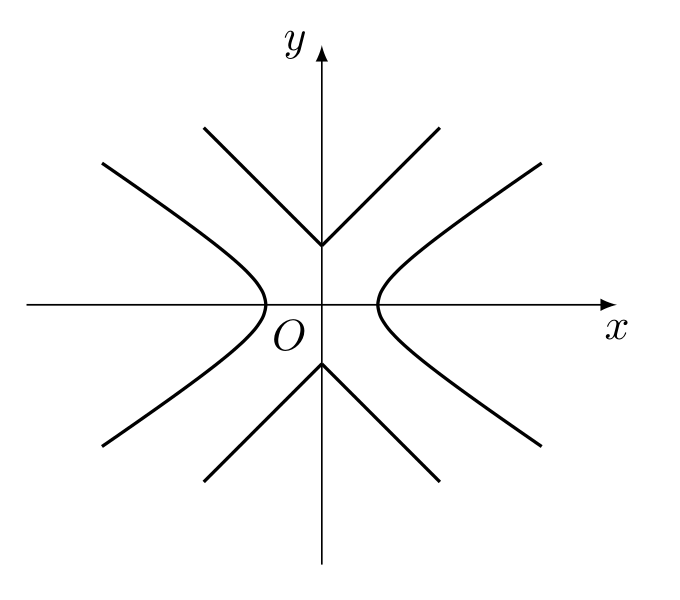
\includegraphics[width=8.0cm]{GaoKao/images/2013/shanghai_science/q22_fig1.png}
\end{center}

        \item 给定常数 \(c>0\)，定义函数 \(f(x)=2|x+c+4|-|x+c|\)，数列 \(a_1\)，\(a_2\)，\(a_3\)，\(\ldots\) 满足 \(a_{n+1}=f(a_n)\)，\(n\in \mathbf{N}^*\).
\begin{enumerate}
\item 若 \(a_1=-c-2\)，求 \(a_2\) 及 \(a_3\)；
\item 求证：对任意 \(n\in \mathbf{N}^*\)，\(a_{n+1}-a_n\geqslant c\)；
\item 是否存在 \(a_1\)，使得 \(a_1\)，\(a_2\)，\(\cdots\)，\(a_n\)，\(\cdots\) 成等差数列？ 若存在，求出所有这样的 \(a_1\)，若不存在，说明理由.
\end{enumerate}

    \end{enumerate}

\end{description}


\subsection{2013年上海卷（文）}\label{gk:2013年上海卷（文）}

\begin{description}

    \item[一、填空题]

    \begin{enumerate}[leftmargin=5pt]

        \item 不等式 \(\frac{x}{2x - 1} < 0\) 的解为\rule[-0.3ex]{3em}{0.4pt}.

        \item 在等差数列 \(\{a_n\}\) 中，若 \(a_1 + a_2 + a_3 + a_4 = 30\)，则 \(a_2 + a_3 =\rule[-0.3ex]{3em}{0.4pt}.\)

        \item 设 \(m \in \mathbb{R}\)，\(m^2 + m - 2 + \left(m^2 - 1\right)\i\) 是纯虚数，其中 \(\i\) 是虚数单位，则 \(m =\rule[-0.3ex]{3em}{0.4pt}.\)

        \item 若 \(\begin{vmatrix} x & 2 \\ 1 & 1 \end{vmatrix} = 0\)，\(\begin{vmatrix} x & y \\ 1 & 1 \end{vmatrix} = 1\)，则 \(x + y =\rule[-0.3ex]{3em}{0.4pt}.\)

        \item 已知 \(\triangle ABC\) 的内角 \(A\)，\(B\)，\(C\) 所对的边分别是 \(a\)，\(b\)，\(c\). 若 \(a^2 + ab + b^2 - c^2 = 0\)，则角 \(C\) 的大小是\rule[-0.3ex]{3em}{0.4pt}.

        \item 某学校高一年级男生人数占该年级学生人数的 \(40\%\). 在一次考试中，男、女生平均分数分别为 \(75\)，\(80\)，则这次考试该年级学生平均分数为\rule[-0.3ex]{3em}{0.4pt}.

        \item 设常数 \(a \in \mathbb{R}\). 若 \(\left(x^2 + \frac{a}{x}\right)^5\) 的二项展开式中 \(x^7\) 项的系数为 \(-10\)，则 \(a =\rule[-0.3ex]{3em}{0.4pt}.\)

        \item 方程 \(\frac{9}{3^x - 1} + 1 = 3^x\) 的实数解为\rule[-0.3ex]{3em}{0.4pt}.

        \item 若 \(\cos x\cos y+\sin x\sin y=\frac{1}{3}\)，则 \(\cos\left(2x-2y\right)=\)\rule[-0.3ex]{3em}{0.4pt}.

        \item 已知圆柱 \(\Omega\) 的母线长为 \(l\)，底面半径为 \(r\)，\(O\) 是上底面圆心，\(A\)，\(B\) 是下底面圆周上两个不同的点，\(BC\) 是母线，如图. 若直线 \(OA\) 与 \(BC\) 所成角的大小为 \(\frac{\pi}{6}\)，则 \(\frac{l}{r} =\rule[-0.3ex]{3em}{0.4pt}.\)

\begin{center}
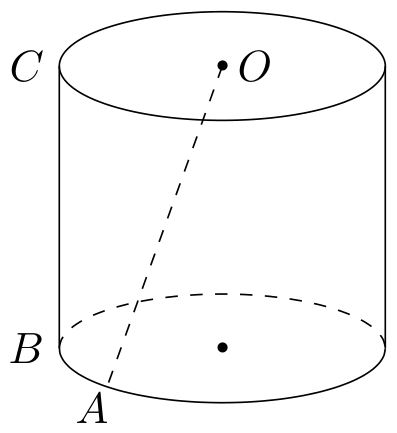
\includegraphics[width=3.2cm]{GaoKao/images/2013/shanghai_liberal/q10_fig1.png}
\end{center}

        \item 盒子中装有编号为 \(1\)，\(2\)，\(3\)，\(4\)，\(5\)，\(6\)，\(7\) 的七个球，从中任意取出两个，则这两个球的编号之积为偶数的概率是\rule[-0.3ex]{3em}{0.4pt}.（结果用最简分数表示）

        \item 设 \(AB\) 是椭圆 \(\Gamma\) 的长轴，点 \(C\) 在 \(\Gamma\) 上，且 \(\angle CBA = \frac{\pi}{4}\)，若 \(AB = 4\)，\(BC = \sqrt{2}\)，则 \(\Gamma\) 的两个焦点之间的距离为\rule[-0.3ex]{3em}{0.4pt}.

        \item 设常数 \(a > 0\). 若 \(9x + \frac{a^2}{x} \geqslant a + 1\) 对一切正实数 \(x\) 成立，则 \(a\) 的取值范围为\rule[-0.3ex]{3em}{0.4pt}.

        \item 已知正方形 \(ABCD\) 的边长为 \(1\). 记以 \(A\) 为起点，其余顶点为终点的向量分别为 \(\bm{a}_1\)，\(\bm{a}_2\)，\(\bm{a}_3\)；以 \(C\) 为起点，其余顶点为终点的向量分别为 \(\bm{c}_1\)，\(\bm{c}_2\)，\(\bm{c}_3\). 若 \(i\)，\(j\)，\(k\)，\(l \in \{1, 2, 3\}\) 且 \(i \neq j\)，\(k \neq l\)，则 \(\left(\bm{a}_i + \bm{a}_j\right) \cdot \left(\bm{c}_k + \bm{c}_l\right)\) 的最小值是\rule[-0.3ex]{3em}{0.4pt}.

    \end{enumerate}

\end{description}

\begin{description}

    \item[二、选择题]

    \begin{enumerate}[leftmargin=5pt]

      \addtocounter{enumi}{+14}

        \item 函数 \(f(x) = x^2 - 1\) （\(x \geqslant 1\)）的反函数为 \(f^{-1}(x)\)，则 \(f^{-1}(2)\) 的值是（\(\quad\)）

        {\centering\begin{tabular*}{\linewidth}{@{}@{\extracolsep{\fill}}llll@{}}
          \text{A. }\(\sqrt{3}\)  &  \text{B. }\(-\sqrt{3}\)  &  \text{C. }\(1 + \sqrt{2}\)  &  \text{D. }\(1 - \sqrt{2}\)
        \end{tabular*}\par}

        \item 设常数 \(a \in \mathbb{R}\)，集合 \(A = \{x \mid \left(x - 1\right)\left(x - a\right) \geqslant 0\}\)，\(B = \{x \mid x \geqslant a - 1\}\). 若 \(A \cup B = \mathbb{R}\)，则 \(a\) 的取值范围为（\(\quad\)）

        {\centering\begin{tabular*}{\linewidth}{@{}@{\extracolsep{\fill}}llll@{}}
          \text{A. }\(\left(-\infty, 2\right)\)  &  \text{B. }\(\left(-\infty, 2\right]\)  &  \text{C. }\(\left(2, +\infty\right)\)  &  \text{D. }\(\left[2, +\infty\right)\)
        \end{tabular*}\par}

        \item 钱大姐常说“便宜没好货”，她这句话的意思是：“不便宜”是“好货”的（\(\quad\)）

        {\centering\begin{tabular*}{\linewidth}{@{}@{\extracolsep{\fill}}llll@{}}
          \text{A. }充分条件  &  \text{B. }必要条件  &  \text{C. }充分必要条件  &  \text{D. }既非充分也非必要条件
        \end{tabular*}\par}

        \item 记椭圆 \(\frac{x^2}{4} + \frac{ny^2}{4n + 1} = 1\) 围成的区域（含边界）为 \(\Omega_n\) （\(n = 1, 2, \cdots\)），当点 \(\left(x, y\right)\) 分别在 \(\Omega_1\)，\(\Omega_2\)，\(\cdots\) 上时，\(x + y\) 的最大值分别是 \(M_1\)，\(M_2\)，\(\cdots\)，则 \(\displaystyle\lim_{n \to \infty} M_n =\)（\(\quad\)）

        {\centering\begin{tabular*}{\linewidth}{@{}@{\extracolsep{\fill}}llll@{}}
          \text{A. }\(0\)  &  \text{B. }\(\frac{1}{4}\)  &  \text{C. }\(2\)  &  \text{D. }\(2\sqrt{2}\)
        \end{tabular*}\par}

    \end{enumerate}

\end{description}

\begin{description}

    \item[三、解答题]

    \begin{enumerate}[leftmargin=5pt]

      \addtocounter{enumi}{+18}

        \item 如图，正三棱锥 \(O - ABC\) 底面边长为 \(2\)，高为 \(1\)，求该三棱锥的体积及表面积.

\begin{center}
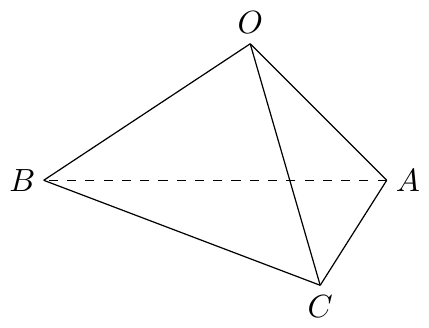
\includegraphics[width=6.8cm]{GaoKao/images/2013/shanghai_liberal/q19_fig1.png}
\end{center}

        \item 甲厂以 \(x\text{ 千克/小时}\) 的速度匀速生产某种产品（生产条件要求 \(1 \leqslant x \leqslant 10\)），每一小时可获得的利润是 \(100\left(5x + 1 - \frac{3}{x}\right)\text{ 元}\).

\begin{enumerate}
\item 求证：生产 \(a\text{ 千克}\) 该产品所获得的利润为 \(100a\left(5 + \frac{1}{x} - \frac{3}{x^2}\right)\text{ 元}\)；
\item 要使生产 \(900\text{ 千克}\) 该产品获得的利润最大，问：甲厂应该选取何种生产速度？并求最大利润.
\end{enumerate}

        \item 已知函数 \(f(x) = 2\sin \omega x\). 其中常数 \(\omega > 0\).

\begin{enumerate}
\item 令 \(\omega = 1\)，判断函数 \(F(x) = f(x) + f\left(x + \frac{\pi}{2}\right)\) 的奇偶性并说明理由；
\item 令 \(\omega = 2\)，将函数 \(y = f(x)\) 的图象向左平移 \(\frac{\pi}{6}\) 个单位，再向上平移 \(1\) 个单位，得到函数 \(y = g(x)\) 的图象. 对任意的 \(a \in \mathbb{R}\)，求 \(y = g(x)\) 在区间 \([a, a + 10\pi]\) 上零点个数的所有可能值.
\end{enumerate}

        \item 已知函数 \(f(x) = 2 - |x|\)，无穷数列 \(\{a_n\}\) 满足 \(a_{n+1} = f(a_n)\)，\(n \in \mathbb{N}^*\).

\begin{enumerate}
\item 若 \(a_1 = 0\)，求 \(a_2\)，\(a_3\)，\(a_4\)；
\item 若 \(a_1 > 0\)，且 \(a_1\)，\(a_2\)，\(a_3\) 成等比数列，求 \(a_1\) 的值；
\item 是否存在 \(a_1\)，使得 \(a_1\)，\(a_2\)，\(a_3\)，\(\cdots\)，\(a_n\)，\(\cdots\) 成等差数列？若存在，求出所有这样的 \(a_1\)；若不存在，说明理由.
\end{enumerate}

        \item 如图，已知双曲线 \(C_1: \frac{x^2}{2} - y^2 = 1\)，曲线 \(C_2: |y| = |x| + 1\). \(P\) 是平面内一点，若存在过点 \(P\) 的直线 \(l\) 与 \(C_1\)，\(C_2\) 都有公共点，则称 \(P\) 为“\(C_1 - C_2\) 型点”.

\begin{enumerate}
\item 在正确证明 \(C_1\) 的左焦点是“\(C_1 - C_2\) 型点”时，要使用一条过该焦点的直线，试写出一条这样的直线的方程（不要求验证）；
\item 设直线 \(y = kx\) 与 \(C_2\) 有公共点. 求证 \(|k| > 1\)，进而证明原点不是“\(C_1 - C_2\) 型点”；
\item 求证：圆 \(x^2 + y^2 = \frac{1}{2}\) 内的点都不是“\(C_1 - C_2\) 型点”.
\end{enumerate}

\begin{center}
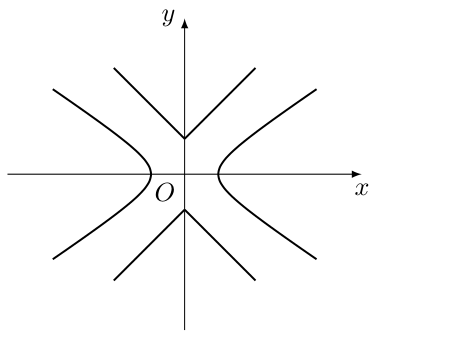
\includegraphics[width=6.5cm]{GaoKao/images/2013/shanghai_liberal/q23_fig1.png}
\end{center}

    \end{enumerate}

\end{description}


\subsection{2013年四川卷（理）}\label{gk:2013年四川卷（理）}

\begin{description}

    \item[一、选择题]

    \begin{enumerate}[leftmargin=5pt]

        \item 设集合 \(A = \{x \mid x + 2 = 0\}\)，集合 \(B = \{x \mid x^2 - 4 = 0\}\)，则 \(A \cap B =\)（\quad）

        {\centering\begin{tabular*}{\linewidth}{@{}@{\extracolsep{\fill}}llll@{}}
          \text{A. }\(\{-2\}\)  &  \text{B. }\(\{2\}\)  &  \text{C. }\(\{-2,2\}\)  &  \text{D. }\(\varnothing\)
        \end{tabular*}\par}

        \item 如图，在复平面内，点 \(A\) 表示复数 \(z\)，则图中表示 \(z\) 的共轭复数的点是（\quad）

\begin{center}
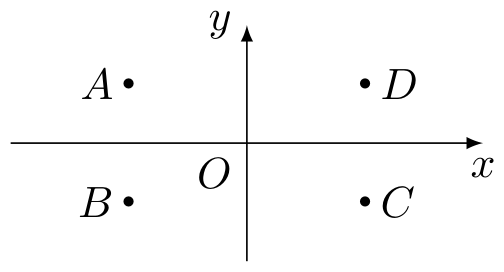
\includegraphics[width=6.2cm]{GaoKao/images/2013/sichuan_science/q2_fig1.png}
\end{center}

        {\centering\begin{tabular*}{\linewidth}{@{}@{\extracolsep{\fill}}llll@{}}
          \text{A. }\(A\)  &  \text{B. }\(B\)  &  \text{C. }\(C\)  &  \text{D. }\(D\)
        \end{tabular*}\par}

        \item 一个几何体的三视图如图所示，则该几何体的直观图可以是（\quad）

\begin{center}
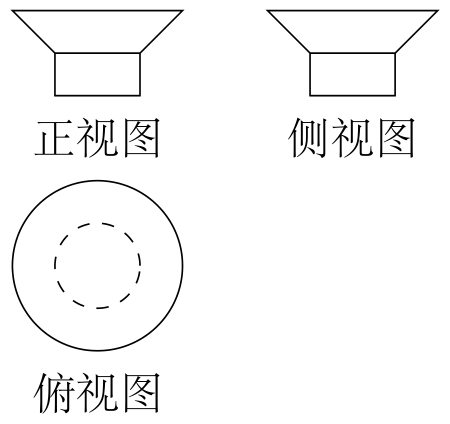
\includegraphics[width=4.6cm]{GaoKao/images/2013/sichuan_science/q3_fig1.png}
\end{center}

        {\centering\begin{tabular*}{\linewidth}{@{}@{\extracolsep{\fill}}cccc@{}}
          \text{A. }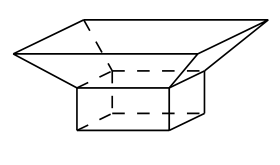
\includegraphics[width=0.15\paperwidth]{GaoKao/images/2013/sichuan_science/q3_optA.png}  &  \text{B. }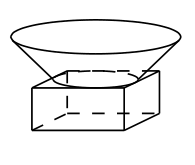
\includegraphics[width=0.15\paperwidth]{GaoKao/images/2013/sichuan_science/q3_optB.png}  &  \text{C. }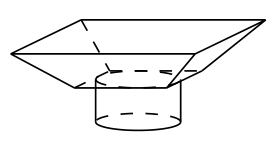
\includegraphics[width=0.15\paperwidth]{GaoKao/images/2013/sichuan_science/q3_optC.png}  &  \text{D. }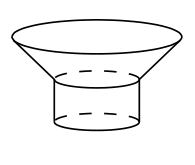
\includegraphics[width=0.15\paperwidth]{GaoKao/images/2013/sichuan_science/q3_optD.png}
        \end{tabular*}\par}

        \item 设 \(x \in \mathbb{Z}\)，集合 \(A\) 是奇数集，集合 \(B\) 是偶数集. 若命题 \(p\)：\(\forall x \in A\)，\(2x \in B\)，则（\quad）

        {\centering\begin{tabular*}{\linewidth}{@{}@{\extracolsep{\fill}}llll@{}}
          \text{A. }\(\neg p\)：\(\forall x \in A\)，\(2x \notin B\)  &  \text{B. }\(\neg p\)：\(\forall x \notin A\)，\(2x \notin B\)  &  \text{C. }\(\neg p\)：\(\exists x \notin A\)，\(2x \in B\)  &  \text{D. }\(\neg p\)：\(\exists x \in A\)，\(2x \notin B\)
        \end{tabular*}\par}

        \item 函数 \( f(x) = 2\sin\left(\omega x + \varphi\right) \)（\(\omega > 0\)，\(-\frac{\pi}{2} < \varphi < \frac{\pi}{2}\)）的部分图象如图所示，则 \(\omega\)，\(\varphi\) 的值分别是（\quad）

\begin{center}
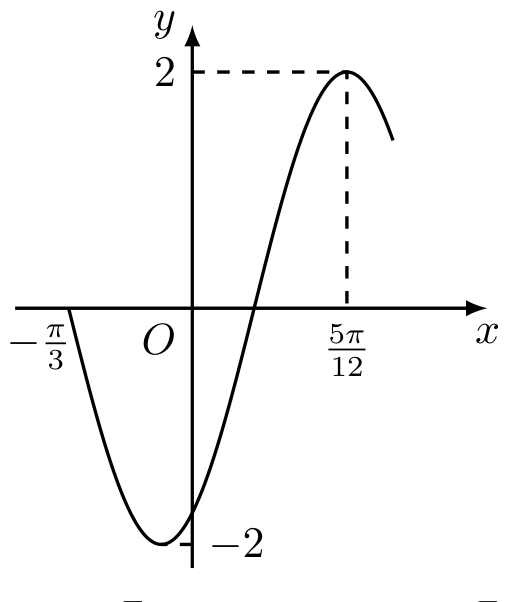
\includegraphics[width=6.3cm]{GaoKao/images/2013/sichuan_science/q5_fig1.png}
\end{center}

        {\centering\begin{tabular*}{\linewidth}{@{}@{\extracolsep{\fill}}llll@{}}
          \text{A. }\(2\)，\(-\frac{\pi}{3}\)  &  \text{B. }\(2\)，\(-\frac{\pi}{6}\)  &  \text{C. }\(4\)，\(-\frac{\pi}{6}\)  &  \text{D. }\(4\)，\(\frac{\pi}{3}\)
        \end{tabular*}\par}

        \item 抛物线 \( y^{2} = 4x \) 的焦点到双曲线 \( x^{2} - \frac{y^{2}}{3} = 1 \) 的渐近线的距离是（\quad）

        {\centering\begin{tabular*}{\linewidth}{@{}@{\extracolsep{\fill}}llll@{}}
          \text{A. }\( \frac{1}{2} \)  &  \text{B. }\(\frac{\sqrt{3}}{2}\)  &  \text{C. }\(1\)  &  \text{D. }\(\sqrt{3}\)
        \end{tabular*}\par}

        \item 函数 \( y = \frac{x^3}{3^{x} - 1} \) 的图象大致是（\quad）

        {\centering\begin{tabular*}{\linewidth}{@{}@{\extracolsep{\fill}}cccc@{}}
          \text{A. }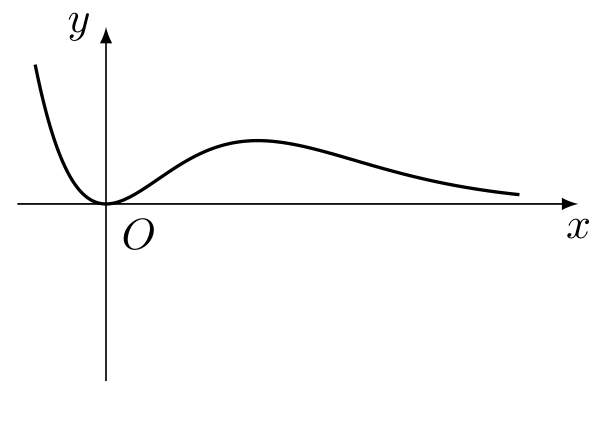
\includegraphics[width=0.15\paperwidth]{GaoKao/images/2013/sichuan_science/q7_optA.png}  &  \text{B. }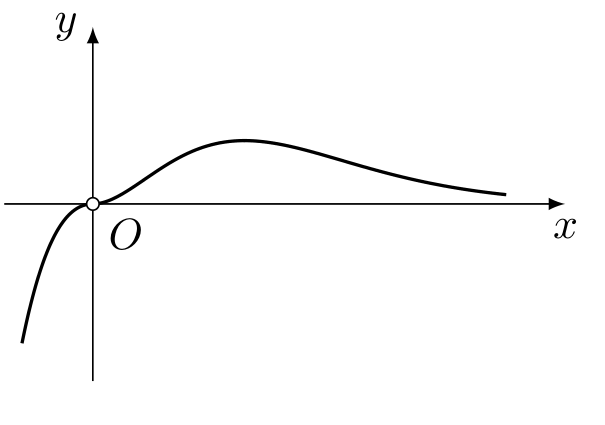
\includegraphics[width=0.15\paperwidth]{GaoKao/images/2013/sichuan_science/q7_optB.png}  &  \text{C. }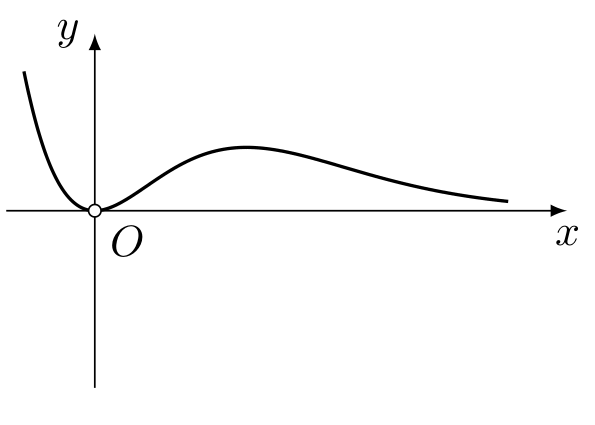
\includegraphics[width=0.15\paperwidth]{GaoKao/images/2013/sichuan_science/q7_optC.png}  &  \text{D. }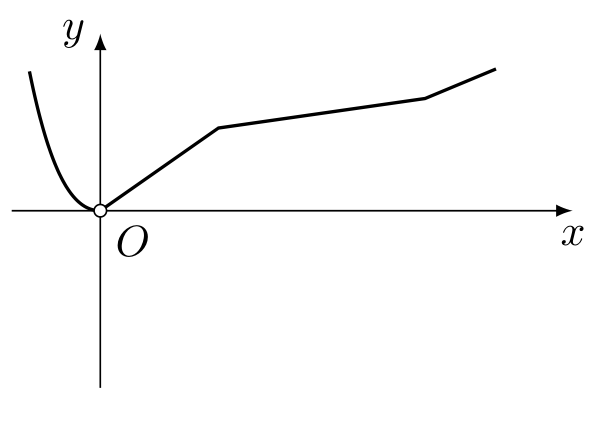
\includegraphics[width=0.15\paperwidth]{GaoKao/images/2013/sichuan_science/q7_optD.png}
        \end{tabular*}\par}

        \item 从 \(1\)，\(3\)，\(5\)，\(7\)，\(9\) 这五个数中，每次取出两个不同的数分别为 \(a\)，\(b\)，共可得到 \( \lg a - \lg b \) 的不同值的个数是（\quad）

        {\centering\begin{tabular*}{\linewidth}{@{}@{\extracolsep{\fill}}llll@{}}
          \text{A. }\(9\)  &  \text{B. }\(10\)  &  \text{C. }\(18\)  &  \text{D. }\(20\)
        \end{tabular*}\par}

        \item 节日前夕，小李在家门前的树上挂了两串彩灯，这两串彩灯的第一次闪亮相互独立，且都在通电后的 \(4\text{ 秒}\) 内任一时刻等可能发生，然后每串彩灯以 \(4\text{ 秒}\) 为间隔闪亮. 那么这两串彩灯同时通电后，它们第一次闪亮的时刻相差不超过 \(2\text{ 秒}\) 的概率是（\quad）

        {\centering\begin{tabular*}{\linewidth}{@{}@{\extracolsep{\fill}}llll@{}}
          \text{A. }\(\frac{1}{4}\)  &  \text{B. }\( \frac{1}{2} \)  &  \text{C. }\( \frac{3}{4} \)  &  \text{D. }\( \frac{7}{8} \)
        \end{tabular*}\par}

        \item 设函数 \( f(x) = \sqrt{{\mathrm{e}}^x + x - a} \) （\( a \in \mathbb{R} \)，\( {\mathrm{e}} \) 为自然对数的底数）. 若曲线 \( y = \sin x \) 上存在 \( (x_0, y_0) \) 使得 \( f(f(y_0)) = y_0 \)，则 \( a \) 的取值范围是（\quad）

        {\centering\begin{tabular*}{\linewidth}{@{}@{\extracolsep{\fill}}llll@{}}
          \text{A. }\([1, {\mathrm{e}}]\)  &  \text{B. }\([{\mathrm{e}}^{-1} - 1, 1]\)  &  \text{C. }\([1, 1 + {\mathrm{e}}]\)  &  \text{D. }\([{\mathrm{e}}^{-1} - 1, {\mathrm{e}} + 1]\)
        \end{tabular*}\par}

    \end{enumerate}

\end{description}

\begin{description}

    \item[二、填空题]

    \begin{enumerate}[leftmargin=5pt]

      \addtocounter{enumi}{+10}

        \item 二项式 \((x + y)^5\) 的展开式中，含 \(x^2 y^3\) 的项的系数是\rule[-0.3ex]{3em}{0.4pt}.（用数字作答）

        \item 在平行四边形 \(ABCD\) 中，对角线 \(AC\) 与 \(BD\) 交于点 \(O\)，\(\overrightarrow{AB} + \overrightarrow{AD} = \lambda \overrightarrow{AO}\)，则 \(\lambda =\)\rule[-0.3ex]{3em}{0.4pt}.

        \item 设 \(\sin 2\alpha = -\sin \alpha\)，\(\alpha \in \left(\frac{\pi}{2}, \pi\right)\)，则 \(\tan 2\alpha\) 的值是\rule[-0.3ex]{3em}{0.4pt}.

        \item 已知 \( f(x) \) 是定义域为 \( \mathbb{R} \) 的偶函数，当 \( x \geqslant 0 \) 时，\( f(x) = x^2 - 4x \)，那么，不等式 \( f(x + 2) < 5 \) 的解集是\rule[-0.3ex]{3em}{0.4pt}.

        \item 设 \(P_1\)，\(P_2\)，\(\cdots\)，\(P_n\) 为平面 \(\alpha\) 内的 \(n\) 个点，在平面 \(\alpha\) 内的所有点中，若点 \(P\) 到 \(P_1\)，\(P_2\)，\(\cdots\)，\(P_n\) 点的距离之和最小，则称点 \(P\) 为 \(P_1\)，\(P_2\)，\(\cdots\)，\(P_n\) 点的一个“中位点”. 例如，线段 \(AB\) 上的任意点都是端点 \(A\)，\(B\) 的中位点. 则有下列命题：

\begin{enumerate}
\item 若三个点 \(A\)，\(B\)，\(C\) 共线，\(C\) 在线段 \(AB\) 上，则 \(C\) 是 \(A\)，\(B\)，\(C\) 的中位点；
\item 直角三角形斜边的中点是该直角三角形三个顶点的中位点；
\item 若四个点 \(A\)，\(B\)，\(C\)，\(D\) 共线，则它们的中位点存在且唯一；
\item 梯形对角线的交点是该梯形四个顶点的唯一中位点.
\end{enumerate}

其中的真命题是\rule[-0.3ex]{3em}{0.4pt}.（写出所有真命题的序号）

    \end{enumerate}

\end{description}

\begin{description}

    \item[三、解答题]

    \begin{enumerate}[leftmargin=5pt]

      \addtocounter{enumi}{+15}

        \item 在等差数列 \(\{a_{n}\}\) 中，\(a_{1} + a_{3} = 8\)，且 \(a_{4}\) 为 \(a_{2}\) 和 \(a_{9}\) 的等比中项，求数列 \(\{a_{n}\}\) 的首项，公差及前 \(n\) 项和.

        \item 在 \(\triangle ABC\) 中，角 \(A\)，\(B\)，\(C\) 的对边分别为 \(a\)，\(b\)，\(c\)，且 \(2\cos^2\frac{A - B}{2}\cos B - \sin (A - B)\sin B + \cos (A + C) = -\frac{3}{5}\).
\begin{enumerate}
\item 求 \(\cos A\) 的值；
\item 若 \(a = 4\sqrt{2}\)，\(b = 5\)，求向量 \(\overrightarrow{BA}\) 在 \(\overrightarrow{BC}\) 方向上的投影.
\end{enumerate}

        \item 某算法的程序框图如图所示，其中输入的变量 \(x\) 在 \(1\)，\(2\)，\(3\)，\(\cdots\)，\(24\) 这 24 个整数中等可能随机产生.

\begin{enumerate}
\item 分别求出按程序框图正确编程运行时输出 \(y\) 的值为 \(i\) 的概率 \(P_{i}\) （\(i = 1, 2, 3\)）；
\item 甲，乙两同学依据自己对程序框图的理解，各自编写程序重复运行 \(n\) 次后，统计记录了输出 \(y\) 的值为 \(i\) （\(i = 1, 2, 3\)） 的频数. 以下是甲，乙所作频数统计表的部分数据. 当 \(n = 2100\) 时，根据表中的数据，分别写出甲，乙所编程序各自输出 \(y\) 的值为 \(i\) （\(i = 1, 2, 3\)） 的频率（用分数表示），并判断两位同学中哪一位所编写程序符合算法要求的可能性较大；

\begin{center}
甲的频数统计表（部分）
\renewcommand{\arraystretch}{1.2}
\begin{tabular}{c|ccc}
\hline
\begin{tabular}{c}运行次数\\\(n\)\end{tabular} & \begin{tabular}{c}输出 \(y\) 的值为\\1 的频数\end{tabular} & \begin{tabular}{c}输出 \(y\) 的值为\\2 的频数\end{tabular} & \begin{tabular}{c}输出 \(y\) 的值为\\3 的频数\end{tabular} \\
\hline
30 & 14 & 6 & 10 \\
\hline
\(\cdots\) & \(\cdots\) & \(\cdots\) & \(\cdots\) \\
\hline
2100 & 1027 & 376 & 697 \\
\hline
\end{tabular}
\end{center}

\begin{center}
乙的频数统计表（部分）
\renewcommand{\arraystretch}{1.2}
\begin{tabular}{c|ccc}
\hline
\begin{tabular}{c}运行次数\\\(n\)\end{tabular} & \begin{tabular}{c}输出 \(y\) 的值为\\1 的频数\end{tabular} & \begin{tabular}{c}输出 \(y\) 的值为\\2 的频数\end{tabular} & \begin{tabular}{c}输出 \(y\) 的值为\\3 的频数\end{tabular} \\
\hline
30 & 12 & 11 & 7 \\
\hline
\(\cdots\) & \(\cdots\) & \(\cdots\) & \(\cdots\) \\
\hline
2100 & 1051 & 696 & 353 \\
\hline
\end{tabular}
\end{center}

\item 按程序框图正确编写的程序运行 3 次，求输出 \(y\) 的值为 2 的次数 \(\xi\) 的分布列及数学期望.
\end{enumerate}

\begin{center}
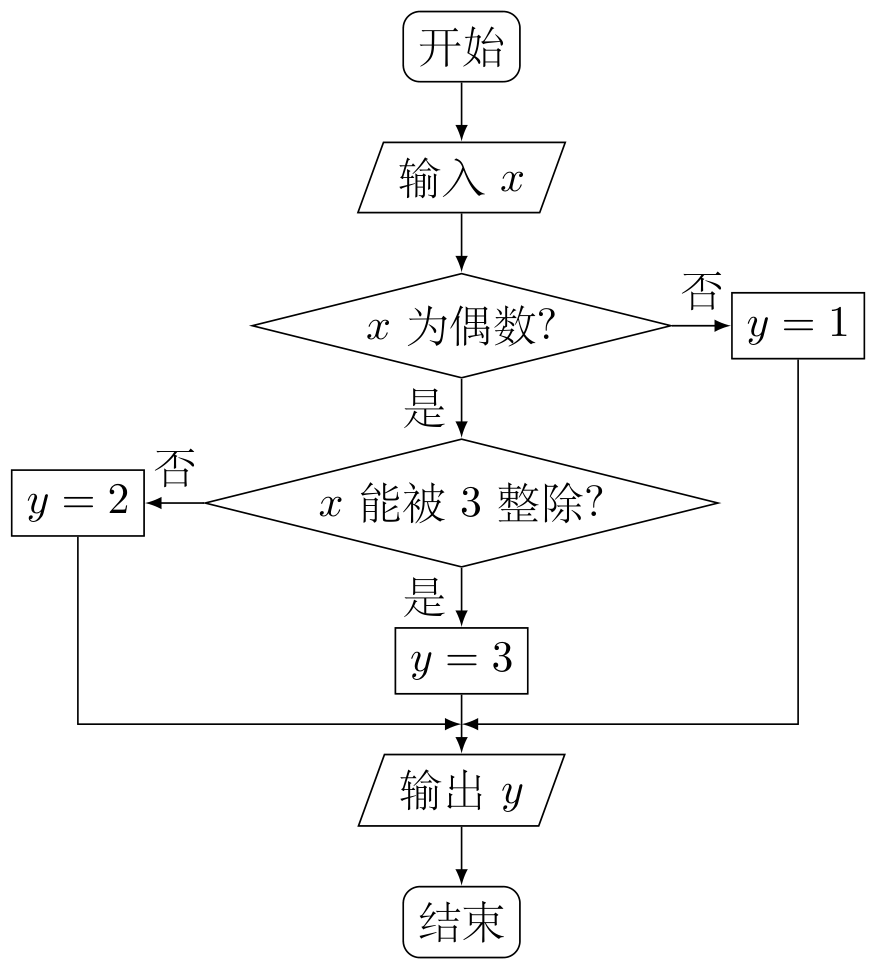
\includegraphics[width=8.5cm]{GaoKao/images/2013/sichuan_science/q18_fig1.png}
\end{center}

        \item 如图，在三棱柱 \(ABC - A_{1}B_{1}C_{1}\) 中，侧棱 \(AA_{1} \perp\) 底面 \(ABC\)，\(AB = AC = 2AA_{1}\)，\(\angle BAC = 120^{\circ}\)，\(D\)，\(D_{1}\) 分别是线段 \(BC\)，\(B_{1}C_{1}\) 的中点，\(P\) 是线段 \(AD\) 的中点.
\begin{enumerate}
\item 在平面 \(ABC\) 内，试作出过点 \(P\) 与平面 \(A_{1}BC\) 平行的直线 \(l\)，说明理由，并证明直线 \(l \perp\) 平面 \(ADD_{1}A_{1}\)；
\item 设（1）中的直线 \(l\) 交 \(AB\) 于点 \(M\)，交 \(AC\) 于点 \(N\)，求二面角 \(A-A_{1}M-N\) 的余弦值.
\end{enumerate}
\begin{center}
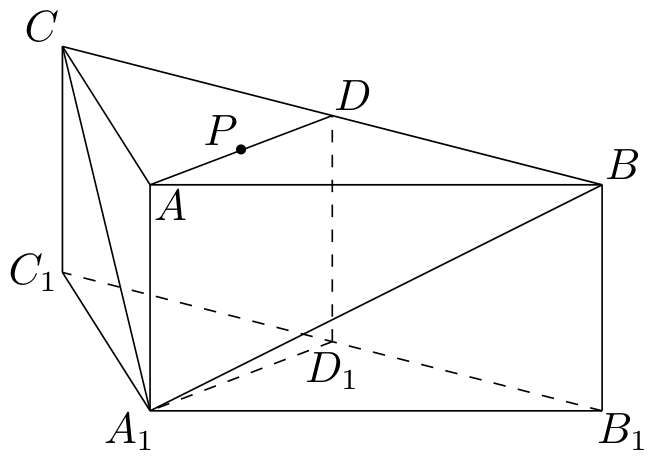
\includegraphics[width=6.3cm]{GaoKao/images/2013/sichuan_science/q19_fig1.png}
\end{center}

        \item 已知椭圆 \(C: \frac{x^2}{a^2} + \frac{y^2}{b^2} = 1\)（\(a>b>0\)）的两个焦点分别为 \(F_1(-1,0)\)，\(F_2(1,0)\)，且椭圆 \(C\) 经过点 \(P\left(\frac{4}{3}, \frac{1}{3}\right)\).
\begin{enumerate}
\item 求椭圆 \(C\) 的离心率；
\item 设过点 \(A(0,2)\) 的直线 \(l\) 与椭圆 \(C\) 交于 \(M\)，\(N\) 两点，点 \(Q\) 是线段 \(MN\) 上的点，且 \(\frac{2}{|AQ|^2} = \frac{1}{|AM|^2} + \frac{1}{|AN|^2}\)，求点 \(Q\) 的轨迹方程.
\end{enumerate}

        \item 已知函数 \( f(x) = \begin{cases}
x^2 + 2x + a, & x < 0,\\
\ln x, & x > 0,
\end{cases} \) 其中 \(a\) 是实数. 设 \( A(x_1, f(x_1))\)，\( B(x_2, f(x_2))\) 为该函数图象上的两点，且 \( x_1 < x_2 \).
\begin{enumerate}
\item 指出函数 \( f(x) \) 的单调区间；
\item 若函数 \( f(x) \) 的图象在点 \(A\)，\(B\) 处的切线互相垂直，且 \( x_{2} < 0 \)，求 \( x_{2} - x_{1} \) 的最小值；
\item 若函数 \( f(x) \) 的图象在点 A，B 处的切线重合，求 \(a\) 的取值范围.
\end{enumerate}

    \end{enumerate}

\end{description}


\subsection{2013年四川卷（文）}\label{gk:2013年四川卷（文）}

\begin{description}

    \item[一、选择题]

    \begin{enumerate}[leftmargin=5pt]

        \item 设集合 \(A = \{1, 2, 3\}\)，集合 \(B = \{-2, 2\}\)，则 \(A \cap B =\)（\quad）

        {\centering\begin{tabular*}{\linewidth}{@{}@{\extracolsep{\fill}}llll@{}}
          \text{A. }\(\varnothing\)  &  \text{B. }\(\{2\}\)  &  \text{C. }\(\{-2, 2\}\)  &  \text{D. }\(\{-2, 1, 2, 3\}\)
        \end{tabular*}\par}

        \item 一个几何体的三视图如图所示，则该几何体可以是（\quad）

\begin{center}
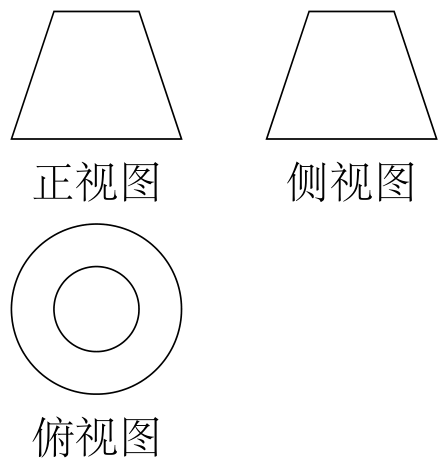
\includegraphics[width=4.4cm]{GaoKao/images/2013/sichuan_liberal/q2_fig1.png}
\end{center}

        {\centering\begin{tabular*}{\linewidth}{@{}@{\extracolsep{\fill}}llll@{}}
          \text{A. }棱柱  &  \text{B. }棱台  &  \text{C. }圆柱  &  \text{D. }圆台
        \end{tabular*}\par}

        \item 如图，在复平面内，点 \(A\) 表示复数 \(z\)，则图中表示 \(z\) 的共轭复数的点是（\quad）

\begin{center}
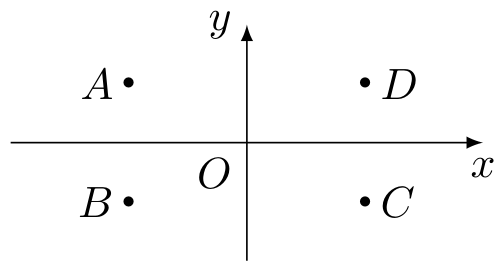
\includegraphics[width=6.2cm]{GaoKao/images/2013/sichuan_liberal/q3_fig1.png}
\end{center}

        {\centering\begin{tabular*}{\linewidth}{@{}@{\extracolsep{\fill}}llll@{}}
          \text{A. }\(A\)  &  \text{B. }\(B\)  &  \text{C. }\(C\)  &  \text{D. }\(D\)
        \end{tabular*}\par}

        \item 设 \(x \in \mathbb{Z}\)，集合 \(A\) 是奇数集，集合 \(B\) 是偶数集. 若命题 \(p: \forall x \in A\)，\(2x \in B\)，则（\quad）

        {\centering\begin{tabular*}{\linewidth}{@{}@{\extracolsep{\fill}}llll@{}}
          \text{A. }\(\neg p: \exists x \in A, 2x \in B\)  &  \text{B. }\(\neg p: \exists x \notin A\)，\(2x \in B\)  &  \text{C. }\(\neg p: \exists x \in A\)，\(2x \notin B\)  &  \text{D. }\(\neg p: \forall x \notin A\)，\(2x \notin B\)
        \end{tabular*}\par}

        \item 抛物线 \(y^{2}=8x\) 的焦点到直线 \(x-\sqrt{3}y=0\) 的距离是（\quad）

        {\centering\begin{tabular*}{\linewidth}{@{}@{\extracolsep{\fill}}llll@{}}
          \text{A. }\(2\sqrt{3}\)  &  \text{B. }\(2\)  &  \text{C. }\(\sqrt{3}\)  &  \text{D. }\(1\)
        \end{tabular*}\par}

        \item 函数 \(f(x)=2\sin\left(\omega x+\varphi\right)\)（\(\omega>0\)，\(-\frac{\pi}{2}<\varphi<\frac{\pi}{2}\)）的部分图象如图所示，则 \(\omega\)，\(\varphi\) 的值分别是（\quad）

\begin{center}
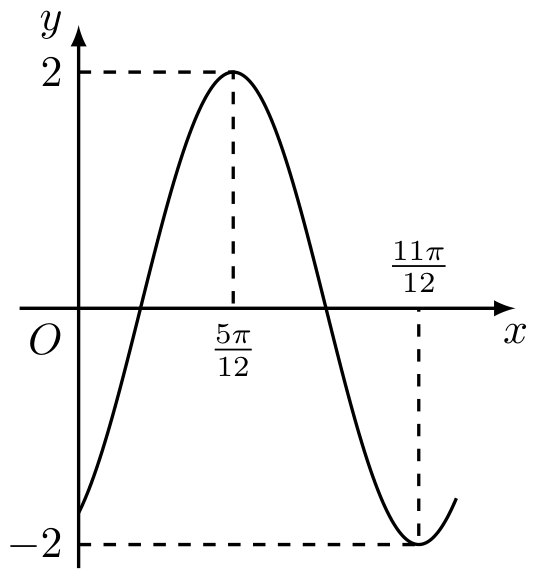
\includegraphics[width=6.7cm]{GaoKao/images/2013/sichuan_liberal/q6_fig1.png}
\end{center}

        {\centering\begin{tabular*}{\linewidth}{@{}@{\extracolsep{\fill}}llll@{}}
          \text{A. }\(2, -\frac{\pi}{3}\)  &  \text{B. }\(2\)，\(-\frac{\pi}{6}\)  &  \text{C. }\(4\)，\(-\frac{\pi}{6}\)  &  \text{D. }\(4\)，\(\frac{\pi}{3}\)
        \end{tabular*}\par}

        \item 某学校随机抽取 20 个班，调查各班中有网上购物经历的人数，所得数据的茎叶图如图所示，以组距为 5 将数据分组成 \([0, 5)\)，\([5, 10)\)，\(\cdots\)，\([30, 35)\)，\([35, 40]\) 时，所作的频率分布直方图是（\quad）
\begin{center}
\begin{tabular}{r|l}
\cline{2-2}
0 & \(7\quad 3\) \\
1 & \(7\quad 6\quad 4\quad 4\quad 3\quad 0\) \\
2 & \(7\quad 5\quad 5\quad 4\quad 3\quad 2\quad 0\) \\
3 & \(8\quad 5\quad 4\quad 3\quad 0\)
\end{tabular}
\end{center}

        {\centering\begin{tabular*}{\linewidth}{@{}@{\extracolsep{\fill}}cccc@{}}
          \text{A. }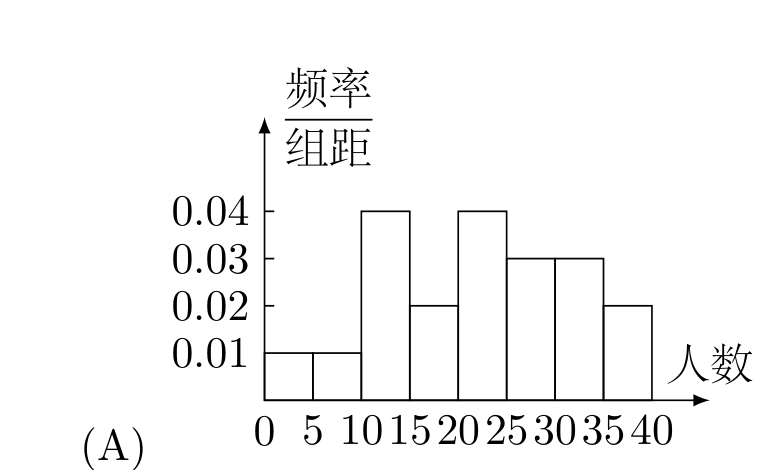
\includegraphics[width=0.15\paperwidth]{GaoKao/images/2013/sichuan_liberal/q7_choice_a.png}  &  \text{B. }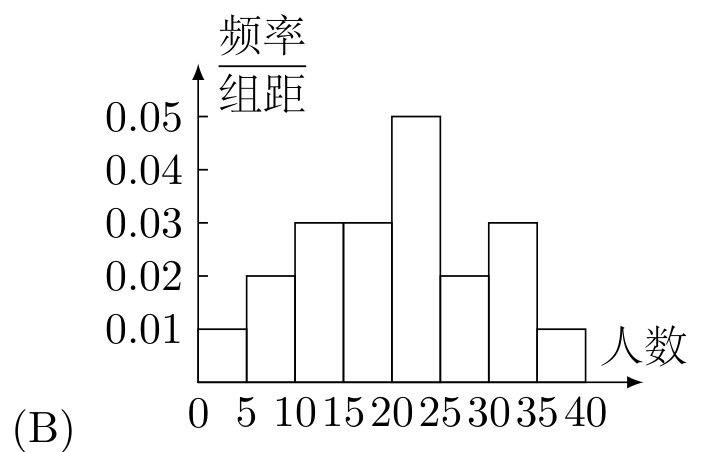
\includegraphics[width=0.15\paperwidth]{GaoKao/images/2013/sichuan_liberal/q7_choice_b.png}  &  \text{C. }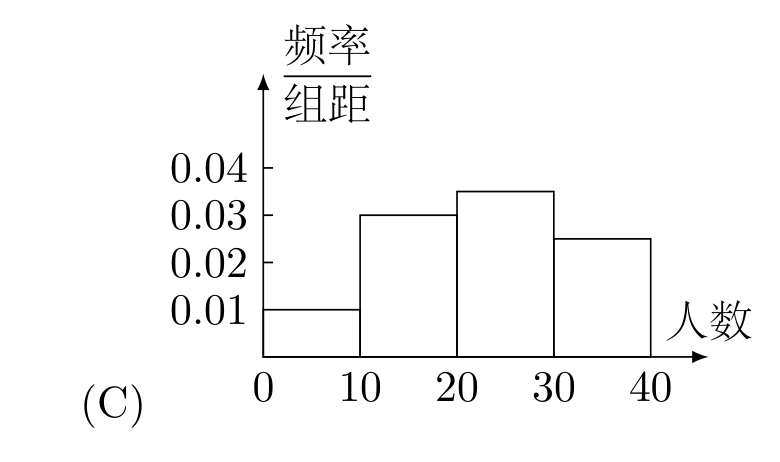
\includegraphics[width=0.15\paperwidth]{GaoKao/images/2013/sichuan_liberal/q7_choice_c.png}  &  \text{D. }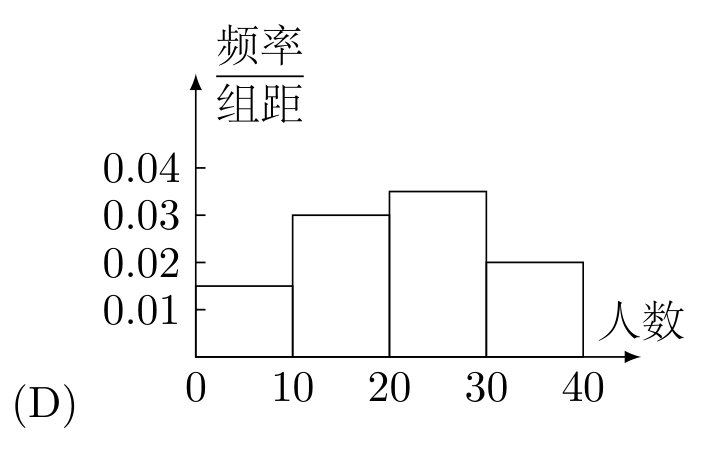
\includegraphics[width=0.15\paperwidth]{GaoKao/images/2013/sichuan_liberal/q7_choice_d.png}
        \end{tabular*}\par}

        \item 若变量 \(x\)，\(y\) 满足约束条件 \(\begin{cases}
x+y\leqslant8,\\
2y-x\leqslant4,\\
x\geqslant0,\\
y\geqslant0
\end{cases}\) 且 \(z=5y-x\) 的最大值为 \(a\)，最小值为 \(b\)，则 \(a-b\) 的值是（\quad）

        {\centering\begin{tabular*}{\linewidth}{@{}@{\extracolsep{\fill}}llll@{}}
          \text{A. }\(48\)  &  \text{B. }\(30\)  &  \text{C. }\(24\)  &  \text{D. }\(16\)
        \end{tabular*}\par}

        \item 从椭圆 \(\frac{x^2}{a^2}+\frac{y^2}{b^2}=1\)（\(a>b>0\)）上一点 \(P\) 向 \(x\) 轴作垂线，垂足恰为左焦点 \(F_1\)，\(A\) 是椭圆与 \(x\) 轴正半轴的交点，\(B\) 是椭圆与 \(y\) 轴正半轴的交点，且 \(AB \parallel OP\)（\(O\) 是坐标原点），则该椭圆的离心率是（\quad）

        {\centering\begin{tabular*}{\linewidth}{@{}@{\extracolsep{\fill}}llll@{}}
          \text{A. }\(\frac{\sqrt{2}}{4}\)  &  \text{B. }\(\frac{1}{2}\)  &  \text{C. }\(\frac{\sqrt{2}}{2}\)  &  \text{D. }\(\frac{\sqrt{3}}{2}\)
        \end{tabular*}\par}

        \item 设函数 \(f(x)=\sqrt{{\mathrm{e}}^x+x-a}\)（\(a\in\mathbb{R}\)，\({\mathrm{e}}\) 为自然对数的底数）. 若存在 \(b\in[0,1]\) 使 \(f(f(b))=b\) 成立，则 \(a\) 的取值范围是（\quad）

        {\centering\begin{tabular*}{\linewidth}{@{}@{\extracolsep{\fill}}llll@{}}
          \text{A. }\([1,{\mathrm{e}}]\)  &  \text{B. }\([1,1+{\mathrm{e}}]\)  &  \text{C. }\([{\mathrm{e}},1+{\mathrm{e}}]\)  &  \text{D. }\([0,1]\)
        \end{tabular*}\par}

    \end{enumerate}

\end{description}

\begin{description}

    \item[二、填空题]

    \begin{enumerate}[leftmargin=5pt]

      \addtocounter{enumi}{+10}

        \item \(\lg\sqrt{5}+\lg\sqrt{20}\) 的值是\rule[-0.3ex]{3em}{0.4pt}.

        \item 在平行四边形 \(ABCD\) 中，对角线 \(AC\) 与 \(BD\) 交于点 \(O\)，\(\overrightarrow{AB}+\overrightarrow{AD}=\lambda\overrightarrow{AO}\)，则 \(\lambda=\)\rule[-0.3ex]{3em}{0.4pt}.

\begin{center}
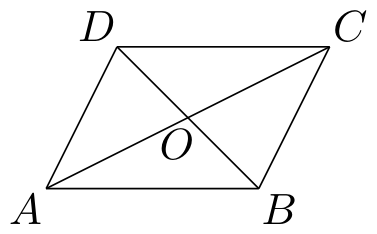
\includegraphics[width=4.7cm]{GaoKao/images/2013/sichuan_liberal/q12_fig1.png}
\end{center}

        \item 已知函数 \(f(x)=4x+\frac{a}{x}\)（\(x>0\)，\(a>0\)）在 \(x=3\) 时取得小值，则 \(a=\)\rule[-0.3ex]{3em}{0.4pt}.

        \item 设 \(\sin 2\alpha=-\sin\alpha\)，\(\alpha\in\left(\frac{\pi}{2},\pi\right)\)，则 \(\tan 2\alpha\) 的值是\rule[-0.3ex]{3em}{0.4pt}.

        \item 在平面直角坐标系内，到点 \(A(1,2)\)，\(B(1,5)\)，\(C(3,6)\)，\(D(7,-1)\) 的距离之和最小的点的坐标是\rule[-0.3ex]{3em}{0.4pt}.

    \end{enumerate}

\end{description}

\begin{description}

    \item[三、解答题]

    \begin{enumerate}[leftmargin=5pt]

      \addtocounter{enumi}{+15}

        \item 在等比数列 \(\{a_n\}\) 中，\(a_2-a_1=2\)，且 \(2a_2\) 为 \(3a_1\) 和 \(a_3\) 的等差中项，求数列 \(\{a_n\}\) 的首项，公比及前 \(n\) 项和.

        \item 在 \(\triangle ABC\) 中，角 \(A\)，\(B\)，\(C\) 的对边分别为 \(a\)，\(b\)，\(c\)，且 \(\cos\left(A-B\right)\cos B-\sin\left(A-B\right)\sin\left(A+C\right)=-\frac35\).
\begin{enumerate}
\item 求 \(\sin A\) 的值；
\item 若 \(a=4\sqrt2\)，\(b=5\)，求向量 \(\overrightarrow{BA}\) 在 \(\overrightarrow{BC}\) 方向上的投影.
\end{enumerate}

        \item 某算法的程序框图如图所示，其中输入的变量 \(x\) 在 \(1\)，\(2\)，\(3\)，\(\cdots\)，\(24\) 这 24 个整数中等可能随机产生.

\begin{enumerate}
\item 分别求出按程序框图正确编程运行时输出 \(y\) 的值为 \(i\) 的概率 \(P_i\)（\(i=1\)，\(2\)，\(3\)）；
\item 甲，乙两同学依据自己对程序框图的理解，各自编写程序重复运行 \(n\) 次后，统计记录了输出 \(y\) 的值为 \(i\)（\(i=1\)，\(2\)，\(3\)）的频数. 以下是甲，乙所作频数统计表的部分数据.

\begin{center}
甲的频数统计表（部分）
\renewcommand{\arraystretch}{1.2}
\begin{tabular}{c|ccc}
\hline
\begin{tabular}{c}运行次数\\\(n\)\end{tabular} & \begin{tabular}{c}输出 \(y\) 的值为\\1 的频数\end{tabular} & \begin{tabular}{c}输出 \(y\) 的值为\\2 的频数\end{tabular} & \begin{tabular}{c}输出 \(y\) 的值为\\3 的频数\end{tabular} \\
\hline
30 & 14 & 6 & 10 \\
\hline
\(\cdots\) & \(\cdots\) & \(\cdots\) & \(\cdots\) \\
\hline
2100 & 1027 & 376 & 697 \\
\hline
\end{tabular}
\end{center}

\begin{center}
乙的频数统计表（部分）
\renewcommand{\arraystretch}{1.2}
\begin{tabular}{c|ccc}
\hline
\begin{tabular}{c}运行次数\\\(n\)\end{tabular} & \begin{tabular}{c}输出 \(y\) 的值为\\1 的频数\end{tabular} & \begin{tabular}{c}输出 \(y\) 的值为\\2 的频数\end{tabular} & \begin{tabular}{c}输出 \(y\) 的值为\\3 的频数\end{tabular} \\
\hline
30 & 12 & 11 & 7 \\
\hline
\(\cdots\) & \(\cdots\) & \(\cdots\) & \(\cdots\) \\
\hline
2100 & 1051 & 696 & 353 \\
\hline
\end{tabular}
\end{center}

当 \(n=2100\) 时，根据表中的数据，分别写出甲，乙所编程序各自输出 \(y\) 的值为 \(i\)（\(i=1\)，\(2\)，\(3\)）的频率（用分数表示），并判断两位同学中哪一位所编写程序符合算法要求的可能性较大.
\end{enumerate}

\begin{center}
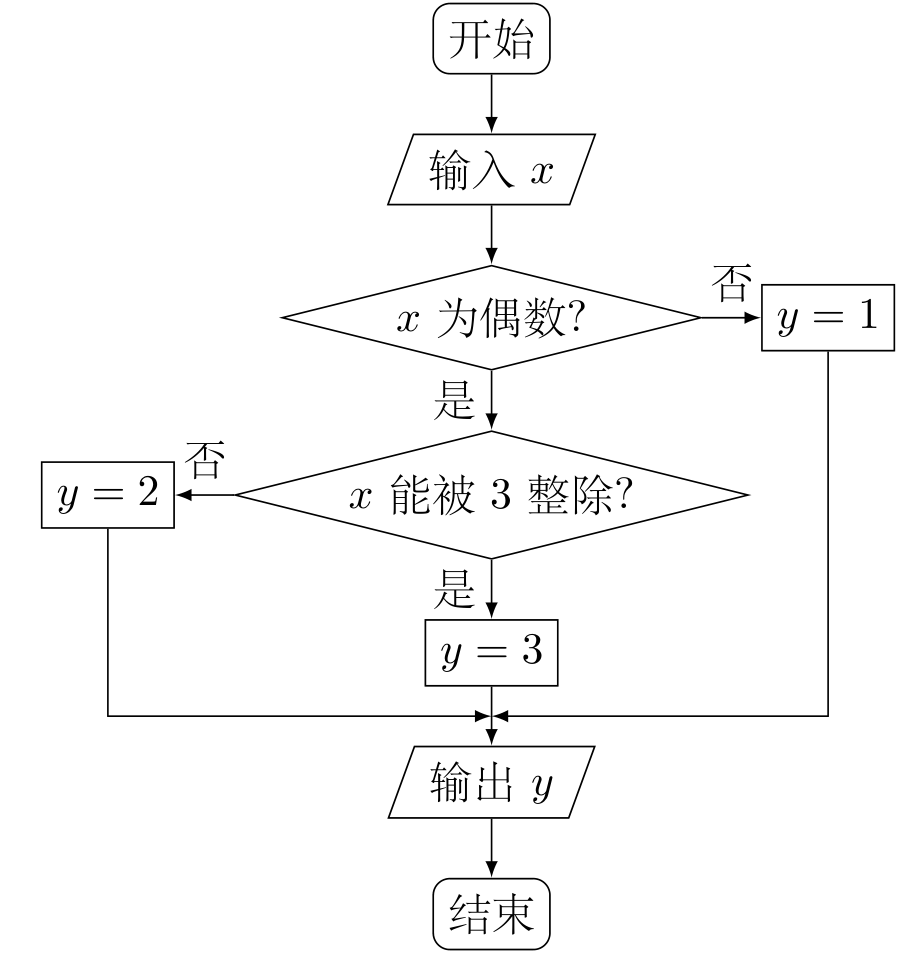
\includegraphics[width=0.48\linewidth]{GaoKao/images/2013/sichuan_liberal/q18_fig1.png}
\end{center}

        \item 如图，在三棱柱 \(ABC-A_{1}B_{1}C_{1}\) 中，侧棱 \(AA_{1}\perp\) 底面 \(ABC\)，\(AB=AC=2AA_{1}=2\)，\(\angle BAC=120^{\circ}\)，\(D\)，\(D_{1}\) 分别是线段 \(BC\)，\(B_{1}C_{1}\) 的中点，点 \(P\) 是线段 \(AD\) 上异于端点的点.
\begin{enumerate}
\item 在平面 \(ABC\) 内，试作出过点 \(P\) 与平面 \(A_{1}BC\) 平行的直线 \(l\)，请说明理由，并证明直线 \(l\perp\) 平面 \(ADD_{1}A_{1}\)；
\item 设（1）中的直线 \(l\) 交 \(AC\) 于点 \(Q\). 求三棱锥 \(A_{1}-QC_{1}D\) 的体积. （锥体体积公式：\(V=\frac13Sh\)，其中 \(S\) 为底面面积，\(h\) 为高）
\end{enumerate}
\begin{center}
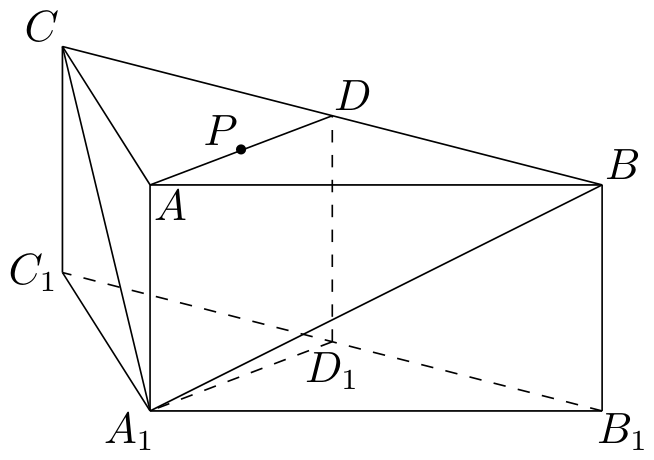
\includegraphics[width=6.3cm]{GaoKao/images/2013/sichuan_liberal/q19_fig1.png}
\end{center}

        \item 已知圆 \(C\) 的方程为 \(x^{2}+\left(y-4\right)^{2}=4\)，点 \(O\) 是坐标原点，直线 \(l:y=kx\) 与圆 \(C\) 交于 \(M\)，\(N\) 两点.
\begin{enumerate}
\item 求 \(k\) 的取值范围；
\item 设 \(Q(m,n)\) 是线段 \(MN\) 上的点，且 \(\dfrac{2}{|OQ|^{2}}=\dfrac{1}{|OM|^{2}}+\dfrac{1}{|ON|^{2}}\)，请将 \(n\) 表示为 \(m\) 的函数.
\end{enumerate}

        \item 已知函数 \(f(x)=\begin{cases}
x^2+2x+a,&x<0,\\
\ln x,&x>0,
\end{cases}\) 其中 \(a\) 是实数. 设 \(A(x_1,f(x_1))\)，\(B(x_2,f(x_2))\) 为该函数图象上的两点，且 \(x_1<x_2\).
\begin{enumerate}
\item 指出函数 \(f(x)\) 的单调区间；
\item 若函数 \(f(x)\) 的图象在点 \(A\)，\(B\) 处的切线互相垂直，且 \(x_2<0\)，证明：\(x_2-x_1\geqslant1\)；
\item 若函数 \(f(x)\) 的图象在点 \(A\)，\(B\) 处的切线重合，求 \(a\) 的取值范围.
\end{enumerate}

    \end{enumerate}

\end{description}


\subsection{2013年山东卷（理）}\label{gk:2013年山东卷（理）}

\begin{description}

    \item[一、选择题]

    \begin{enumerate}[leftmargin=5pt]

        \item 复数 \(z\) 满足 \((z - 3)(2 - \i) = 5\)（\(\i\) 为虚数单位），则 \(z\) 的共轭复数 \(\overline{z}\) 为（\quad）

        {\centering\begin{tabular*}{\linewidth}{@{}@{\extracolsep{\fill}}llll@{}}
          \text{A. }\(2 + \i\)  &  \text{B. }\(2 - \i\)  &  \text{C. }\(5 + \i\)  &  \text{D. }\(5 - \i\)
        \end{tabular*}\par}

        \item 设集合 \(A = \{0, 1, 2\}\)，则集合 \(B = \{x - y \mid x \in A, y \in A\}\) 中元素的个数是（\quad）

        {\centering\begin{tabular*}{\linewidth}{@{}@{\extracolsep{\fill}}llll@{}}
          \text{A. }\(1\)  &  \text{B. }\(3\)  &  \text{C. }\(5\)  &  \text{D. }\(9\)
        \end{tabular*}\par}

        \item 已知函数 \(f(x)\) 为奇函数，且当 \(x > 0\) 时，\(f(x) = x^2 + \frac{1}{x}\)，则 \(f(-1) =\)（\quad）

        {\centering\begin{tabular*}{\linewidth}{@{}@{\extracolsep{\fill}}llll@{}}
          \text{A. }\(-2\)  &  \text{B. }\(0\)  &  \text{C. }\(1\)  &  \text{D. }\(2\)
        \end{tabular*}\par}

        \item 已知三棱柱 \(ABC - A_{1}B_{1}C_{1}\) 的侧棱与底面垂直，体积为 \(\frac{9}{4}\)，底面是边长为 \(\sqrt{3}\) 的正三角形，若 \(P\) 为底面 \(A_{1}B_{1}C_{1}\) 的中心，则 \(PA\) 与平面 \(ABC\) 所成角的大小为（\quad）

        {\centering\begin{tabular*}{\linewidth}{@{}@{\extracolsep{\fill}}llll@{}}
          \text{A. }\(\frac{5\pi}{12}\)  &  \text{B. }\(\frac{\pi}{3}\)  &  \text{C. }\(\frac{\pi}{4}\)  &  \text{D. }\(\frac{\pi}{6}\)
        \end{tabular*}\par}

        \item 将函数 \(y = \sin (2x + \varphi)\) 的图象沿 \(x\) 轴向左平移 \(\frac{\pi}{8}\) 个单位后，得到一个偶函数的图象，则 \(\varphi\) 的一个可能取值为（\quad）

        {\centering\begin{tabular*}{\linewidth}{@{}@{\extracolsep{\fill}}llll@{}}
          \text{A. }\(\frac{3\pi}{4}\)  &  \text{B. }\(\frac{\pi}{4}\)  &  \text{C. }\(0\)  &  \text{D. }\(-\frac{\pi}{4}\)
        \end{tabular*}\par}

        \item 在平面直角坐标系 \(xOy\) 中，\(M\) 为不等式组
\(\begin{cases}
2x - y - 2 \geqslant 0,\\
x + 2y - 1 \geqslant 0,\\
3x + y - 8 \leqslant 0
\end{cases}\)
所表示的区域上一动点，则直线 \(OM\) 斜率的最小值为（\quad）

        {\centering\begin{tabular*}{\linewidth}{@{}@{\extracolsep{\fill}}llll@{}}
          \text{A. }\(2\)  &  \text{B. }\(1\)  &  \text{C. }\(-\frac{1}{3}\)  &  \text{D. }\(-\frac{1}{2}\)
        \end{tabular*}\par}

        \item 给定两个命题 \(p\)，\(q\). 若 \(\neg p\) 是 \(q\) 的必要而不充分条件，则 \(p\) 是 \(\neg q\) 的（\quad）

        {\centering\begin{tabular*}{\linewidth}{@{}@{\extracolsep{\fill}}llll@{}}
          \text{A. }充分而不必要条件  &  \text{B. }必要而不充分条件  &  \text{C. }充要条件  &  \text{D. }既不充分也不必要条件
        \end{tabular*}\par}

        \item 函数 \(y = x \cos x + \sin x\) 的图象大致为（\quad）

        {\centering\begin{tabular*}{\linewidth}{@{}@{\extracolsep{\fill}}cccc@{}}
          \text{A. }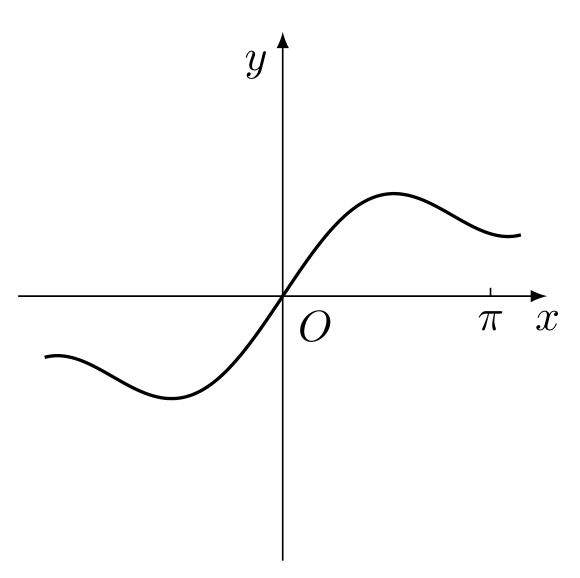
\includegraphics[width=0.15\paperwidth]{GaoKao/images/2013/shandong_science/q8_optA.png}  &  \text{B. }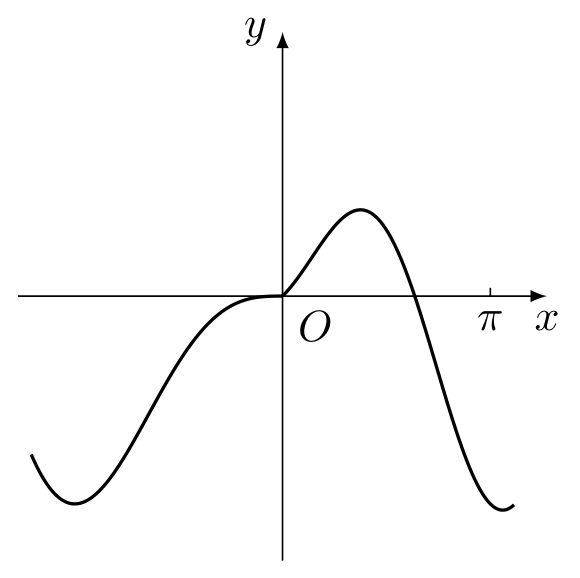
\includegraphics[width=0.15\paperwidth]{GaoKao/images/2013/shandong_science/q8_optB.png}  &  \text{C. }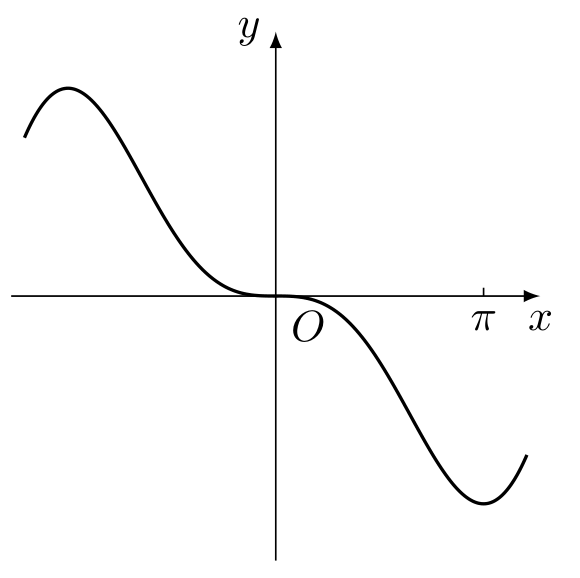
\includegraphics[width=0.15\paperwidth]{GaoKao/images/2013/shandong_science/q8_optC.png}  &  \text{D. }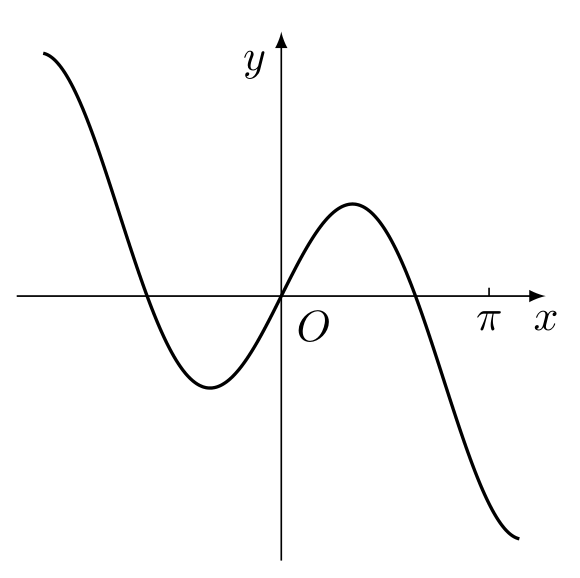
\includegraphics[width=0.15\paperwidth]{GaoKao/images/2013/shandong_science/q8_optD.png}
        \end{tabular*}\par}

        \item 过点 \((3,1)\) 作圆 \((x - 1)^2 + y^2 = 1\) 的两条切线，切点分别为 \(A\)，\(B\)，则直线 \(AB\) 的方程为（\quad）

        {\centering\begin{tabular*}{\linewidth}{@{}@{\extracolsep{\fill}}llll@{}}
          \text{A. }\(2x + y - 3 = 0\)  &  \text{B. }\(2x - y - 3 = 0\)  &  \text{C. }\(4x - y - 3 = 0\)  &  \text{D. }\(4x + y - 3 = 0\)
        \end{tabular*}\par}

        \item 用 \(0\)，\(1\)，\(\ldots\)，\(9\) 十个数字，可以组成有重复数字的三位数的个数为（\quad）

        {\centering\begin{tabular*}{\linewidth}{@{}@{\extracolsep{\fill}}llll@{}}
          \text{A. }\(243\)  &  \text{B. }\(252\)  &  \text{C. }\(261\)  &  \text{D. }\(279\)
        \end{tabular*}\par}

        \item 抛物线 \(C_{1}: y = \frac{1}{2p}x^2\)（\(p > 0\)）的焦点与双曲线 \(C_{2}: \frac{x^2}{3} - y^2 = 1\) 的右焦点的连线交 \(C_{1}\) 于第一象限的点 \(M\). 若 \(C_{1}\) 在点 \(M\) 处的切线平行于 \(C_{2}\) 的一条渐近线，则 \(p =\)（\quad）

        {\centering\begin{tabular*}{\linewidth}{@{}@{\extracolsep{\fill}}llll@{}}
          \text{A. }\(\frac{\sqrt{3}}{16}\)  &  \text{B. }\(\frac{\sqrt{3}}{8}\)  &  \text{C. }\(\frac{2\sqrt{3}}{3}\)  &  \text{D. }\(\frac{4\sqrt{3}}{3}\)
        \end{tabular*}\par}

        \item 设正实数 \(x\)，\(y\)，\(z\) 满足 \(x^2 - 3xy + 4y^2 - z = 0\)，则当 \(\frac{xy}{z}\) 取得最大值时，\(\frac{2}{x} + \frac{1}{y} - \frac{2}{z}\) 的最大值为（\quad）

        {\centering\begin{tabular*}{\linewidth}{@{}@{\extracolsep{\fill}}llll@{}}
          \text{A. }\(0\)  &  \text{B. }\(1\)  &  \text{C. }\(\frac{9}{4}\)  &  \text{D. }\(3\)
        \end{tabular*}\par}

    \end{enumerate}

\end{description}

\begin{description}

    \item[二、填空题]

    \begin{enumerate}[leftmargin=5pt]

      \addtocounter{enumi}{+12}

        \item 执行如下的程序框图，若输入的 \(\varepsilon\) 的值为 \(0.25\)，则输出的 \(n\) 的值为\rule[-0.3ex]{3em}{0.4pt}.

\begin{center}
\begin{center}
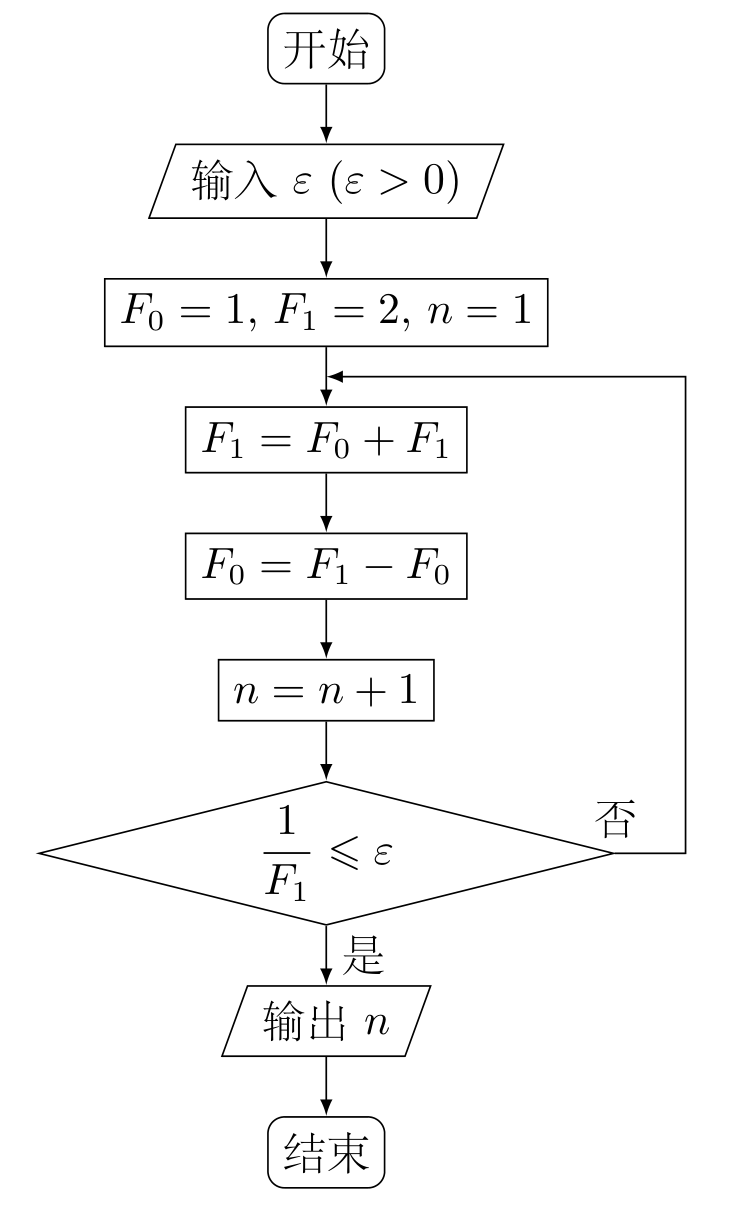
\includegraphics[width=5.5cm]{GaoKao/images/2013/shandong_science/q13_fig1.png}
\end{center}
\end{center}

        \item 在区间 \([-3,3]\) 上随机取一个数 \(x\)，使得 \(|x + 1| - |x - 2| \geqslant 1\) 成立的概率为\rule[-0.3ex]{3em}{0.4pt}.

        \item 已知向量 \(\overrightarrow{AB}\) 与 \(\overrightarrow{AC}\) 的夹角为 \(120^\circ\)，且 \(|\overrightarrow{AB}| = 3\)，\(|\overrightarrow{AC}| = 2\). 若 \(\overrightarrow{AP} = \lambda\overrightarrow{AB} + \overrightarrow{AC}\)，且 \(\overrightarrow{AP} \perp \overrightarrow{BC}\)，则实数 \(\lambda\) 的值为\rule[-0.3ex]{3em}{0.4pt}.

        \item 定义“正对数”：\(\ln^+x = \begin{cases}
0, & 0 < x < 1,\\
\ln x, & x \geqslant 1.
\end{cases}\)
现有四个命题：

\begin{enumerate}
\item 若 \(a > 0\)，\(b > 0\)，则 \(\ln^+(a^b) = b\ln^+a\)；
\item 若 \(a > 0\)，\(b > 0\)，则 \(\ln^+(ab) = \ln^+a + \ln^+b\)；
\item 若 \(a > 0\)，\(b > 0\)，则 \(\ln^+\!\left(\frac{a}{b}\right) \geqslant \ln^+a - \ln^+b\)；
\item 若 \(a > 0\)，\(b > 0\)，则 \(\ln^+(a + b) \leqslant \ln^+a + \ln^+b + \ln 2\).
\end{enumerate}

其中真命题有\rule[-0.3ex]{3em}{0.4pt}.（写出所有真命题的编号）

    \end{enumerate}

\end{description}

\begin{description}

    \item[三、解答题]

    \begin{enumerate}[leftmargin=5pt]

      \addtocounter{enumi}{+16}

        \item 设 \(\triangle ABC\) 的内角 \(A\)，\(B\)，\(C\) 所对的边分别为 \(a\)，\(b\)，\(c\)，且 \(a + c = 6\)，\(b = 2\)，\(\cos B = \frac{7}{9}\).
\begin{enumerate}
\item 求 \(a\)，\(c\) 的值；
\item 求 \(\sin (A - B)\) 的值.
\end{enumerate}

        \item 如图所示，在三棱锥 \(P - ABQ\) 中，\(PB \perp\) 平面 \(ABQ\)，\(BA = BP = BQ\)，\(D\)，\(C\)，\(E\)，\(F\) 分别是 \(AQ\)，\(BQ\)，\(AP\)，\(BP\) 的中点，\(AQ = 2BD\)，\(PD\) 与 \(EQ\) 交于点 \(G\)，\(PC\) 与 \(FQ\) 交于点 \(H\)，连接 \(GH\).
\begin{enumerate}
\item 求证：\(AB \parallel GH\)；
\item 求二面角 \(D - GH - E\) 的余弦值.
\end{enumerate}
\begin{center}
\begin{center}
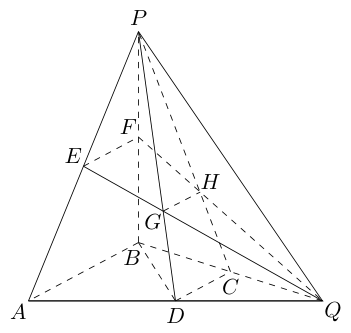
\includegraphics[width=8.0cm]{GaoKao/images/2013/shandong_science/q18_fig1.png}
\end{center}
\end{center}

        \item 甲，乙两支排球队进行比赛，约定先胜 3 局者获得比赛的胜利，比赛随即结束. 除第五局甲队获胜的概率是 \(\frac{1}{2}\) 外，其余每局比赛甲队获胜的概率都是 \(\frac{2}{3}\). 假设每局比赛结果互相独立.
\begin{enumerate}
\item 分别求甲队以 \(3:0\)，\(3:1\)，\(3:2\) 胜利的概率；
\item 若比赛结果为 \(3:0\) 或 \(3:1\)，则胜利方得 \(3\) 分，对方得 \(0\) 分；若比赛结果为 \(3:2\)，则胜利方得 \(2\) 分，对方得 \(1\) 分，求乙队得分 \(X\) 的分布列及数学期望.
\end{enumerate}

        \item 设等差数列 \(\{a_{n}\}\) 的前 \(n\) 项和为 \(S_{n}\)，且 \(S_{4} = 4S_{2}\)，\(a_{2n} = 2a_{n} + 1\).
\begin{enumerate}
\item 求数列 \(\{a_{n}\}\) 的通项公式；
\item 设数列 \(\{b_{n}\}\) 的前 \(n\) 项和 \(T_{n}\)，且 \(T_{n} + \frac{a_{n} + 1}{2^n} = \lambda\)（\(\lambda\) 为常数），令 \(c_{n} = b_{2n}\)（\(n \in \mathbf{N}^*\)）. 求数列 \(\{c_{n}\}\) 的前 \(n\) 项和 \(R_{n}\).
\end{enumerate}

        \item 设函数 \(f(x) = \frac{x}{{\mathrm{e}}^{2x}} + c\)（\({\mathrm{e}} = 2.71828\cdots\) 是自然对数的底数，\(c \in \mathbb{R}\)）.
\begin{enumerate}
\item 求 \(f(x)\) 的单调区间，最大值；
\item 讨论关于 \(x\) 的方程 \(\lvert \ln x \rvert = f(x)\) 的根的个数.
\end{enumerate}

        \item 椭圆 \(C: \frac{x^2}{a^2} + \frac{y^2}{b^2} = 1\)（\(a > b > 0\)）的左，右焦点分别是 \(F_{1}\)，\(F_{2}\)，离心率为 \(\frac{\sqrt{3}}{2}\)，过 \(F_{1}\) 且垂直于 \(x\) 轴的直线被椭圆 \(C\) 截得的线段长为 \(1\).
\begin{enumerate}
\item 求椭圆 \(C\) 的方程；
\item 点 \(P\) 是椭圆 C 上除长轴端点外的任一点，连接 \(PF_{1}\)，\(PF_{2}\). 设 \(\angle F_{1}PF_{2}\) 的角平分线 \(PM\) 交 C 的长轴于点 \(M(m,0)\)，求 \(m\) 的取值范围；
\item 在（2）的条件下，过点 \(P\) 作斜率为 \(k\) 的直线 \(l\)，使得 \(l\) 与椭圆 \(C\) 有且只有一个公共点. 设直线 \(PF_{1}\)，\(PF_{2}\) 的斜率分别为 \(k_{1}\)，\(k_{2}\)，若 \(k \neq 0\)，试证明 \(\frac{1}{kk_{1}} + \frac{1}{kk_{2}}\) 为定值，并求出这个定值.
\end{enumerate}

    \end{enumerate}

\end{description}


\subsection{2013年山东卷（文）}\label{gk:2013年山东卷（文）}

\begin{description}

    \item[一、选择题]

    \begin{enumerate}[leftmargin=5pt]

        \item 复数 \(z = \frac{(2 - \i)^2}{\i}\)（\(\i\) 为虚数单位），则 \(|z| =\)（\quad）

        {\centering\begin{tabular*}{\linewidth}{@{}@{\extracolsep{\fill}}llll@{}}
          \text{A. }25  &  \text{B. }\(\sqrt{41}\)  &  \text{C. }5  &  \text{D. }\(\sqrt{5}\)
        \end{tabular*}\par}

        \item 已知集合 \(A\)，\(B\) 均为全集 \(U = \{1, 2, 3, 4\}\) 的子集，且 \(\complement_U (A \cup B) = \{4\}\)，\(B = \{1, 2\}\)，则 \(A \cap \complement_U B =\)（\quad）

        {\centering\begin{tabular*}{\linewidth}{@{}@{\extracolsep{\fill}}llll@{}}
          \text{A. }\(\{3\}\)  &  \text{B. }\(\{4\}\)  &  \text{C. }\(\{3, 4\}\)  &  \text{D. }\(\varnothing\)
        \end{tabular*}\par}

        \item 已知函数 \( f(x) \) 为奇函数，且当 \( x > 0 \) 时，\( f(x) = x^2 + \frac{1}{x} \)，则 \( f(-1) =\)（\quad）

        {\centering\begin{tabular*}{\linewidth}{@{}@{\extracolsep{\fill}}llll@{}}
          \text{A. }2  &  \text{B. }1  &  \text{C. }0  &  \text{D. }\(-2\)
        \end{tabular*}\par}

        \item 一个四棱锥的侧棱长都相等，底面是正方形，其正（主）视图如图所示，则该四棱锥侧面积和体积分别是（\quad）

\begin{center}
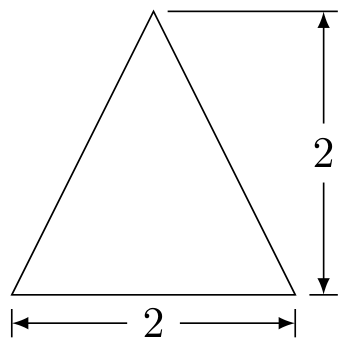
\includegraphics[width=10.1cm]{GaoKao/images/2013/shandong_liberal/q4_fig1.png}
\end{center}

        {\centering\begin{tabular*}{\linewidth}{@{}@{\extracolsep{\fill}}llll@{}}
          \text{A. }\(4\sqrt{5}\)，\(8\)  &  \text{B. }\(4\sqrt{5}\)，\(\frac{8}{3}\)  &  \text{C. }\(4(\sqrt{5} + 1)\)，\(\frac{8}{3}\)  &  \text{D. }\(8\)，\(8\)
        \end{tabular*}\par}

        \item 函数 \( f(x) = \sqrt{1 - 2^x} + \frac{1}{\sqrt{x + 3}} \) 的定义域为（\quad）

        {\centering\begin{tabular*}{\linewidth}{@{}@{\extracolsep{\fill}}llll@{}}
          \text{A. }\((-3,0]\)  &  \text{B. }\((-3, 1]\)  &  \text{C. }\((-\infty, -3) \cup (-3, 0]\)  &  \text{D. }\((-\infty, -3) \cup (-3, 1]\)
        \end{tabular*}\par}

        \item 执行两次如图所示的程序框图，若第一次输入的 \(a\) 的值为 \(-1.2\)，第二次输入的 \(a\) 的值为 \(1.2\)，则第一次，第二次输出的 \(a\) 的值分别为（\quad）

\begin{center}
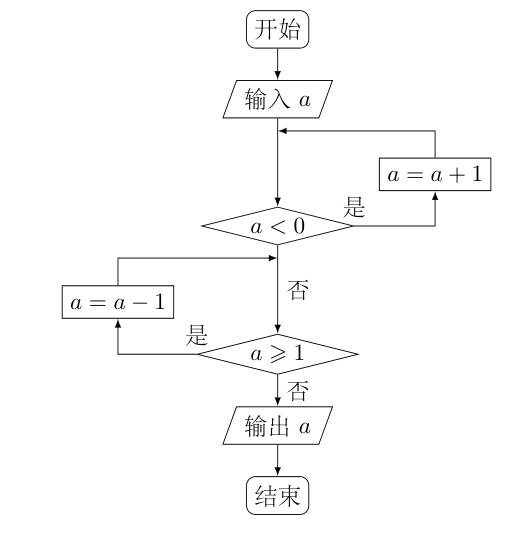
\includegraphics[width=0.40\linewidth]{GaoKao/images/2013/shandong_liberal/q6_fig1.png}
\end{center}

        {\centering\begin{tabular*}{\linewidth}{@{}@{\extracolsep{\fill}}llll@{}}
          \text{A. }\(0.2\)，\(0.2\)  &  \text{B. }\(0.2\)，\(0.8\)  &  \text{C. }\(0.8\)，\(0.2\)  &  \text{D. }\(0.8\)，\(0.8\)
        \end{tabular*}\par}

        \item \(\triangle ABC\) 的内角 \(A\)，\(B\)，\(C\) 所对的边分别是 \(a\)，\(b\)，\(c\). 若 \(B = 2A\)，\(a = 1\)，\(b = \sqrt{3}\)，则 \(c =\)（\quad）

        {\centering\begin{tabular*}{\linewidth}{@{}@{\extracolsep{\fill}}llll@{}}
          \text{A. }\(2 \sqrt{3}\)  &  \text{B. }2  &  \text{C. }\(\sqrt{2}\)  &  \text{D. }1
        \end{tabular*}\par}

        \item 给定两个命题 \( p \)，\( q \)，若 \( \neg p \) 是 \( q \) 的必要而不充分条件，则 \( p \) 是 \( \neg q \) 的（\quad）

        {\centering\begin{tabular*}{\linewidth}{@{}@{\extracolsep{\fill}}llll@{}}
          \text{A. }充分而不必要条件  &  \text{B. }必要而不充分条件  &  \text{C. }充要条件  &  \text{D. }既不充分也不必要条件
        \end{tabular*}\par}

        \item 函数 \( y = x \cos x + \sin x \) 的图象大致为（\quad）

        {\centering\begin{tabular*}{\linewidth}{@{}@{\extracolsep{\fill}}cccc@{}}
          \text{A. }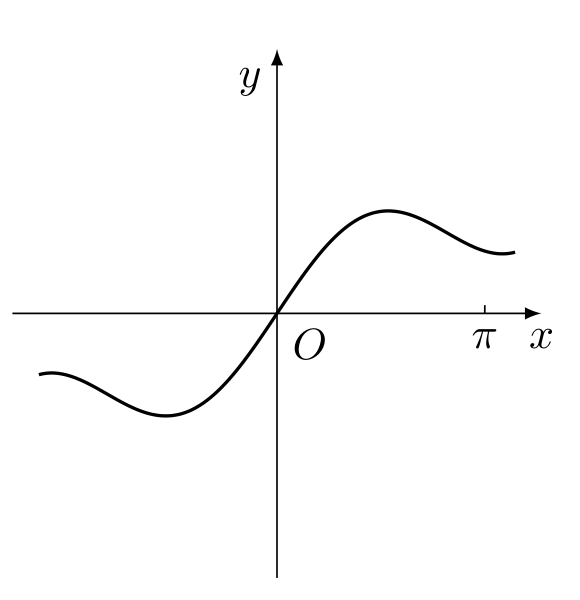
\includegraphics[width=0.15\paperwidth]{GaoKao/images/2013/shandong_liberal/q9_choice_a.png}  &  \text{B. }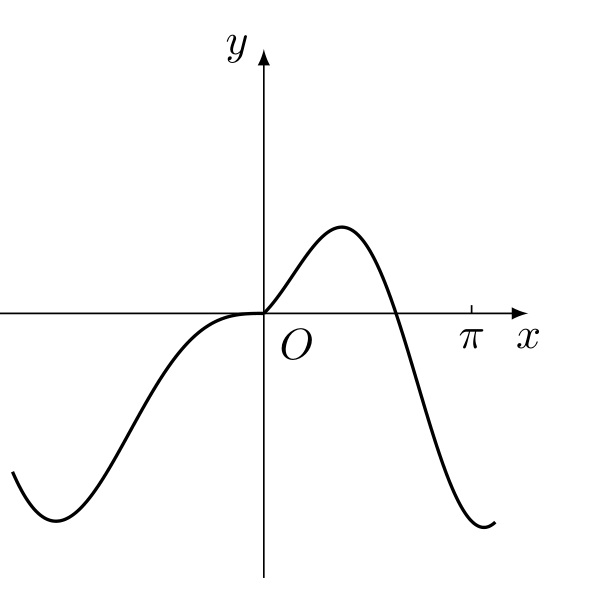
\includegraphics[width=0.15\paperwidth]{GaoKao/images/2013/shandong_liberal/q9_choice_b.png}  &  \text{C. }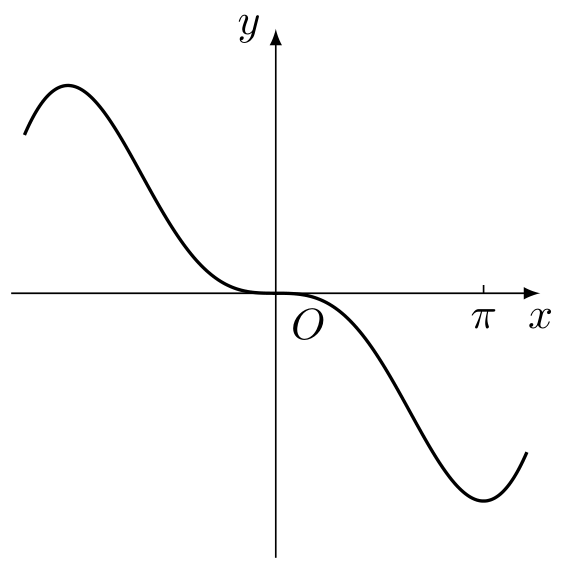
\includegraphics[width=0.15\paperwidth]{GaoKao/images/2013/shandong_liberal/q9_choice_c.png}  &  \text{D. }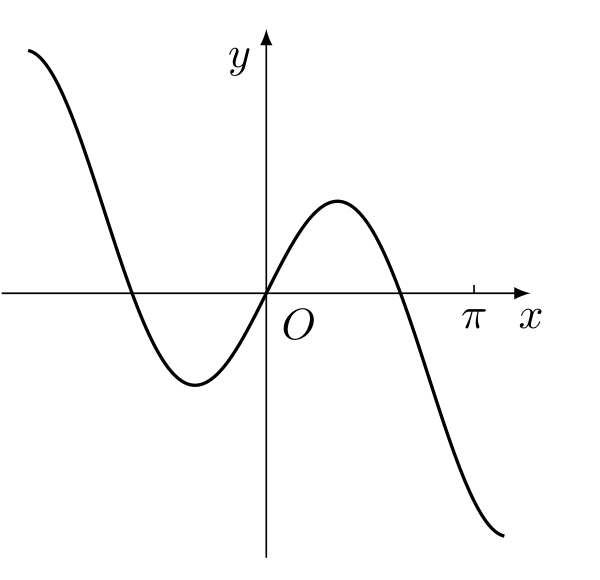
\includegraphics[width=0.15\paperwidth]{GaoKao/images/2013/shandong_liberal/q9_choice_d.png}
        \end{tabular*}\par}

        \item 将某选手的 \(9\) 个得分去掉 \(1\) 个最高分，去掉 \(1\) 个最低分，\(7\) 个剩余分数的平均分为 \(91\)，现场作的 \(9\) 个分数的茎叶图后来有 \(1\) 个数据模糊，无法辨认，在图中以 \(x\) 表示：

\begin{center}
\begin{tabular}{r|l}
8 & \(7\quad 7\) \\
9 & \(4\quad 0\quad 1\quad 0\quad x\quad 9\quad 1\)
\end{tabular}
\end{center}
则 7 个剩余分数的方差为（\quad）

        {\centering\begin{tabular*}{\linewidth}{@{}@{\extracolsep{\fill}}llll@{}}
          \text{A. }\(\frac{116}{9}\)  &  \text{B. }\(\frac{36}{7}\)  &  \text{C. }36  &  \text{D. }\(\frac{6\sqrt{7}}{7}\)
        \end{tabular*}\par}

        \item 抛物线 \(C_1: y = \frac{1}{2p} x^2\)（\(p > 0\)）的焦点与双曲线 \(C_2: \frac{x^2}{3} - y^2 = 1\) 的右焦点的连线交 \(C_1\) 于第一象限的点 \(M\). 若 \(C_1\) 在点 \(M\) 处的切线平行于 \(C_2\) 的一条渐近线，则 \(p =\)（\quad）

        {\centering\begin{tabular*}{\linewidth}{@{}@{\extracolsep{\fill}}llll@{}}
          \text{A. }\(\frac{\sqrt{3}}{16}\)  &  \text{B. }\(\frac{\sqrt{3}}{8}\)  &  \text{C. }\(\frac{2\sqrt{3}}{3}\)  &  \text{D. }\(\frac{4\sqrt{3}}{3}\)
        \end{tabular*}\par}

        \item 设正实数 \(x\)，\(y\)，\(z\) 满足 \(x^2 - 3xy + 4y^2 - z = 0\)，则当 \(\frac{z}{xy}\) 取得最小值时，\(x + 2y - z\) 的最大值为（\quad）

        {\centering\begin{tabular*}{\linewidth}{@{}@{\extracolsep{\fill}}llll@{}}
          \text{A. }0  &  \text{B. }\(\frac{9}{8}\)  &  \text{C. }2  &  \text{D. }\(\frac{9}{4}\)
        \end{tabular*}\par}

    \end{enumerate}

\end{description}

\begin{description}

    \item[二、填空题]

    \begin{enumerate}[leftmargin=5pt]

      \addtocounter{enumi}{+12}

        \item 过点 \((3,1)\) 作圆 \( (x-2)^{2}+(y-2)^{2}=4 \) 的弦，其中最短弦的长为\rule[-0.3ex]{3em}{0.4pt}.

        \item 在平面直角坐标系 \(xOy\) 中，\(M\) 为不等式组 \(\begin{cases}
2x + 3y - 6 \leqslant 0,\\
x + y - 2 \geqslant 0,\\
y \geqslant 0,
\end{cases}\) 所表示的区域上一动点，则 \(|OM|\) 的最小值是\rule[-0.3ex]{3em}{0.4pt}.

        \item 在平面直角坐标系 \(xOy\) 中，已知 \(\overrightarrow{OA} = (-1, t)\)，\(\overrightarrow{OB} = (2, 2)\). 若 \(\angle ABO = 90^\circ\)，则实数 \(t\) 的值为\rule[-0.3ex]{3em}{0.4pt}.

        \item 定义“正对数”： \( \ln^{+} x=\begin{cases}
0,&0<x<1,\\
\ln x,&x\geqslant1
\end{cases} \).
现有四个命题：
\begin{enumerate}
\item 若 \(a > 0\)，\(b > 0\)，则 \( \ln^{+}(a^{b}) = b\ln^{+} a \)；
\item 若 \(a > 0\)，\(b > 0\)，则 \( \ln^{+}(ab) = \ln^{+}a + \ln^{+}b \)；
\item 若 \(a > 0\)，\(b > 0\)，则 \( \ln^{+}\left(\frac{a}{b}\right) \geqslant \ln^{+} a - \ln^{+} b \)；
\item 若 \(a > 0\)，\(b > 0\)，则 \( \ln^{+}(a + b) \leqslant \ln^{+} a + \ln^{+} b + \ln 2 \).
\end{enumerate}

其中真命题有\rule[-0.3ex]{3em}{0.4pt}.（写出所有真命题的编号）

    \end{enumerate}

\end{description}

\begin{description}

    \item[三、解答题]

    \begin{enumerate}[leftmargin=5pt]

      \addtocounter{enumi}{+16}

        \item 某小组共有 A，B，C，D，E 五位同学，他们的身高（单位：米）及体重指标（单位：千克/米\(^{2}\)）如下表所示：

\begin{center}
\begin{tabular}{|c|c|c|c|c|c|}
\hline
 & A & B & C & D & E \\
\hline
身高 & 1.69 & 1.73 & 1.75 & 1.79 & 1.82 \\
\hline
体重指标 & 19.2 & 25.1 & 18.5 & 23.3 & 20.9 \\
\hline
\end{tabular}
\end{center}

\begin{enumerate}
\item 从该小组身高低于 \(1.80\) 的同学中任选 \(2\) 人，求选到的 \(2\) 人身高都在 \(1.78\) 以下的概率；
\item 从该小组同学中任选 \(2\) 人，求选到的 \(2\) 人的身高都在 \(1.70\) 以上且体重指标都在 \([18.5, 23.9)\) 中的概率.
\end{enumerate}

        \item 设函数 \(f(x) = \frac{\sqrt{3}}{2} - \sqrt{3}\sin^2\omega x - \sin \omega x\cos \omega x \)（\(\omega > 0\)），且 \( y = f(x) \) 图象的一个对称中心到最近的对称轴的距离为 \( \frac{\pi}{4} \).

\begin{enumerate}
\item 求 \(\omega\) 的值；
\item 求 \( f(x) \) 在区间 \( \left[\pi, \frac{3\pi}{2}\right] \) 上的最大值和最小值.
\end{enumerate}

        \item 如图，四棱锥 \(P - ABCD\) 中，\(AB \perp AC\)，\(AB \perp PA\)，\(AB \parallel CD\)，\(AB = 2CD\)，\(E\)，\(F\)，\(G\)，\(M\)，\(N\) 分别为 \(PB\)，\(AB\)，\(BC\)，\(PD\)，\(PC\) 的中点.

\begin{enumerate}
\item 求证： \(CE \parallel\) 平面 \(PAD\)；
\item 求证：平面 \(EFG \perp\) 平面 \(EMN\).
\end{enumerate}

\begin{center}
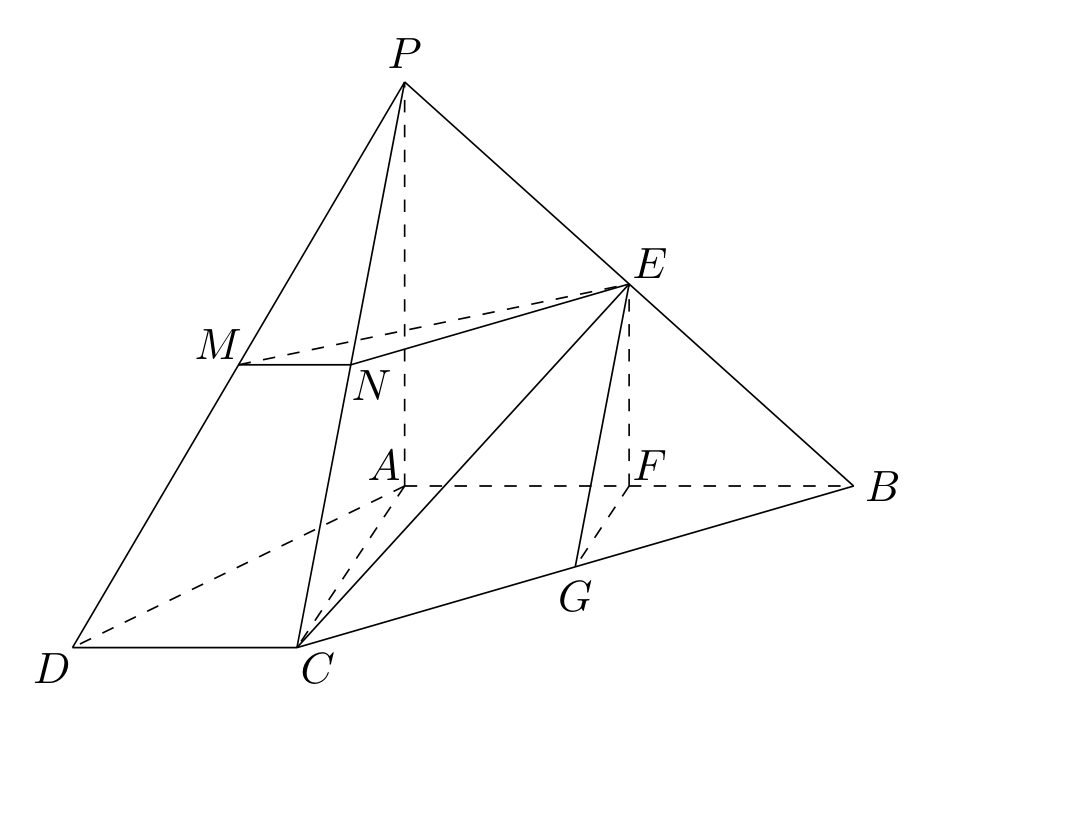
\includegraphics[width=11.0cm]{GaoKao/images/2013/shandong_liberal/q19_fig1.png}
\end{center}

        \item 设等差数列 \(\{a_{n}\}\) 的前 \(n\) 项和为 \(S_{n}\)，且 \(S_{4} = 4S_{2}\)，\(a_{2n} = 2a_{n} + 1\).

\begin{enumerate}
\item 求数列 \( \{a_{n}\} \) 的通项公式；
\item 若数列 \( \{b_{n}\} \) 满足 \(\frac{b_{1}}{a_{1}} + \frac{b_{2}}{a_{2}} + \cdots + \frac{b_{n}}{a_{n}} = 1 - \frac{1}{2^{n}}\)，\(n \in \mathbb{N}^{*}\)，求 \( \{b_{n}\} \) 的前 \(n\) 项和 \( T_{n} \).
\end{enumerate}

        \item 已知函数 \( f(x) = ax^2 + bx - \ln x  \)（\(a, b \in \mathbb{R}\)）.

\begin{enumerate}
\item 设 \(a \geqslant 0\)，求 \(f(x)\) 的单调区间；
\item 设 \(a > 0\)，且对任意 \(x > 0\)，\(f(x) \geqslant f(1)\)，试比较 \(\ln a\) 与 \(-2b\) 的大小.
\end{enumerate}

        \item 在平面直角坐标系 \(xOy\) 中，已知椭圆 \(C\) 的中心在原点 \(O\)，焦点在 \(x\) 轴上，短轴长为 2，离心率为 \(\frac{\sqrt{2}}{2}\).

\begin{enumerate}
\item 求椭圆 \(C\) 的方程；
\item \(A\)，\(B\) 为椭圆 \(C\) 上满足 \(\triangle AOB\) 的面积为 \(\frac{\sqrt{6}}{4}\) 的任意两点，\(E\) 为线段 \(AB\) 的中点，射线 \(OE\) 交椭圆 \(C\) 于点 \(P\). 设 \(\overrightarrow{OP} = t\overrightarrow{OE}\)，求实数 \(t\) 的值.
\end{enumerate}

    \end{enumerate}

\end{description}


\subsection{2013年陕西卷（理）}\label{gk:2013年陕西卷（理）}

\begin{description}

    \item[一、选择题]

    \begin{enumerate}[leftmargin=5pt]

        \item 设全集为 \(\mathbb{R}\)，函数 \(f(x) = \sqrt{1 - x^2}\) 的定义域为 \(M\)，则 \(\complement_{\mathbb{R}} M\) 为（\quad）

        {\centering\begin{tabular*}{\linewidth}{@{}@{\extracolsep{\fill}}llll@{}}
          \text{A. }\(\left[-1, 1\right]\)  &  \text{B. }\(\left(-1, 1\right)\)  &  \text{C. }\(\left(-\infty, -1\right] \cup \left[1, +\infty\right)\)  &  \text{D. }\(\left(-\infty, -1\right) \cup \left(1, +\infty\right)\)
        \end{tabular*}\par}

        \item 根据下列算法语句，当输入 \(x\) 为 \(60\) 时，输出 \(y\) 的值为（\quad）

\begin{center}
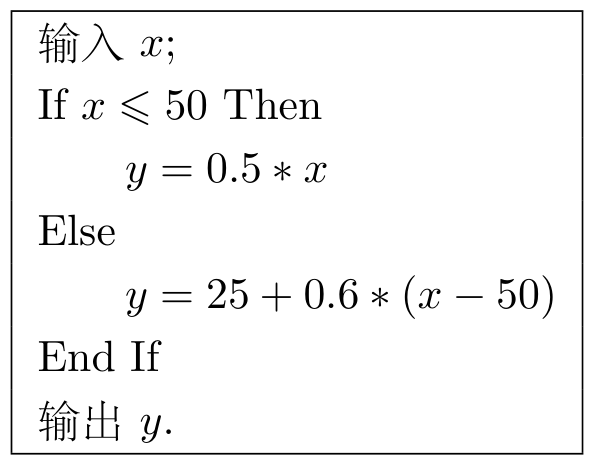
\includegraphics[width=5.7cm]{GaoKao/images/2013/shaanxi_science/q2_fig1.png}
\end{center}

        {\centering\begin{tabular*}{\linewidth}{@{}@{\extracolsep{\fill}}llll@{}}
          \text{A. }\(25\)  &  \text{B. }\(30\)  &  \text{C. }\(31\)  &  \text{D. }\(61\)
        \end{tabular*}\par}

        \item 设 \(\bm{a}\)，\(\bm{b}\) 为向量，则 \(\left|\bm{a}\cdot\bm{b}\right|=\left|\bm{a}\right|\left|\bm{b}\right|\) 是“\(\bm{a}\parallel\bm{b}\)”的（\quad）

        {\centering\begin{tabular*}{\linewidth}{@{}@{\extracolsep{\fill}}llll@{}}
          \text{A. }充分不必要条件  &  \text{B. }必要不充分条件  &  \text{C. }充分必要条件  &  \text{D. }既不充分也不必要条件
        \end{tabular*}\par}

        \item 某单位有 \(840\) 名职工，现采用系统抽样方法，抽取 \(42\) 人做问卷调查，将 \(840\) 人按 \(1\)，\(2\)，\(\cdots\)，\(840\) 随机编号，则抽取的 \(42\) 人中，编号落入区间 \([481,720]\) 的人数为（\quad）

        {\centering\begin{tabular*}{\linewidth}{@{}@{\extracolsep{\fill}}llll@{}}
          \text{A. }\(11\)  &  \text{B. }\(12\)  &  \text{C. }\(13\)  &  \text{D. }\(14\)
        \end{tabular*}\par}

        \item 如图，在矩形区域 \(ABCD\) 的 \(A\)，\(C\) 两点处各有一个通信基站，假设其信号覆盖范围分别是扇形区域 \(ADE\) 和扇形区域 \(CBF\)（该矩形区域内无其他信号来源，基站工作正常）. 若在该矩形区域内随机地选一地点，则该地点无信号的概率是（\quad）

\begin{center}
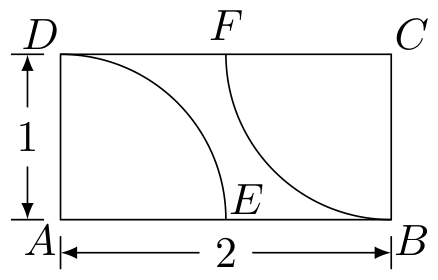
\includegraphics[width=5.4cm]{GaoKao/images/2013/shaanxi_science/q5_fig1.png}
\end{center}

        {\centering\begin{tabular*}{\linewidth}{@{}@{\extracolsep{\fill}}llll@{}}
          \text{A. }\(1-\dfrac{\pi}{4}\)  &  \text{B. }\(\dfrac{\pi}{2}-1\)  &  \text{C. }\(2-\dfrac{\pi}{2}\)  &  \text{D. }\(\dfrac{\pi}{4}\)
        \end{tabular*}\par}

        \item 设 \(z_{1}\)，\(z_{2}\) 是复数，则下列命题中的假命题是（\quad）

        {\centering\begin{tabular*}{\linewidth}{@{}@{\extracolsep{\fill}}llll@{}}
          \text{A. }若 \(\left|z_1-z_2\right|=0\)，则 \(\overline{z_1}=\overline{z_2}\)  &  \text{B. }若 \(z_1=\overline{z_2}\)，则 \(\overline{z_1}=z_2\)  &  \text{C. }若 \(\left|z_1\right|=\left|z_2\right|\)，则 \(z_1\cdot\overline{z_1}=z_2\cdot\overline{z_2}\)  &  \text{D. }若 \(\left|z_1\right|=\left|z_2\right|\)，则 \(z_1^2=z_2^2\)
        \end{tabular*}\par}

        \item 设 \(\triangle ABC\) 的内角 \(A\)，\(B\)，\(C\) 所对的边分别为 \(a\)，\(b\)，\(c\)，若 \(b\cos C+c\cos B=a\sin A\)，则 \(\triangle ABC\) 的形状为（\quad）

        {\centering\begin{tabular*}{\linewidth}{@{}@{\extracolsep{\fill}}llll@{}}
          \text{A. }锐角三角形  &  \text{B. }直角三角形  &  \text{C. }钝角三角形  &  \text{D. }不确定
        \end{tabular*}\par}

        \item 设函数 \(f(x)=\begin{cases}
\left(x-\dfrac{1}{x}\right)^6, & x<0,\\
-\sqrt{x}, & x\geqslant0,
\end{cases}\) 则当 \(x>0\) 时，\(f[f(x)]\) 表达式的展开式中常数项为（\quad）

        {\centering\begin{tabular*}{\linewidth}{@{}@{\extracolsep{\fill}}llll@{}}
          \text{A. }\(-20\)  &  \text{B. }\(20\)  &  \text{C. }\(-15\)  &  \text{D. }\(15\)
        \end{tabular*}\par}

        \item 在如图所示的锐角三角形空地中，欲建一个面积不小于 \(300 \mathrm{~m}^{2}\) 的内接矩形花园（阴影部分），则其边长 \(x\)（单位 \(\mathrm{m}\)）的取值范围是（\quad）

\begin{center}
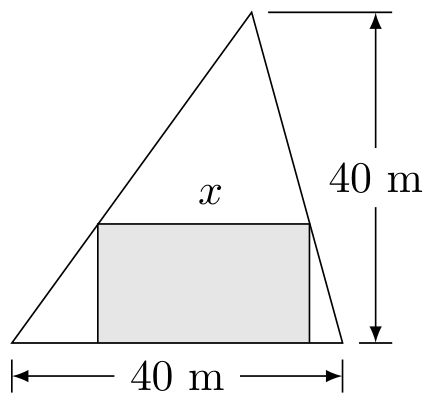
\includegraphics[width=4.2cm]{GaoKao/images/2013/shaanxi_science/q9_fig1.png}
\end{center}

        {\centering\begin{tabular*}{\linewidth}{@{}@{\extracolsep{\fill}}llll@{}}
          \text{A. }\(\left[15,20\right]\)  &  \text{B. }\(\left[12,25\right]\)  &  \text{C. }\(\left[10,30\right]\)  &  \text{D. }\(\left[20,30\right]\)
        \end{tabular*}\par}

        \item 设 \([x]\) 表示不大于 \(x\) 的最大整数，则对任意实数 \(x\)，\(y\)，有（\quad）

        {\centering\begin{tabular*}{\linewidth}{@{}@{\extracolsep{\fill}}llll@{}}
          \text{A. }\(\left[-x\right]=-\left[x\right]\)  &  \text{B. }\(\left[2x\right]=2\left[x\right]\)  &  \text{C. }\(\left[x+y\right]\leqslant\left[x\right]+\left[y\right]\)  &  \text{D. }\(\left[x-y\right]\leqslant\left[x\right]-\left[y\right]\)
        \end{tabular*}\par}

    \end{enumerate}

\end{description}

\begin{description}

    \item[二、填空题]

    \begin{enumerate}[leftmargin=5pt]

      \addtocounter{enumi}{+10}

        \item 双曲线 \(\dfrac{x^2}{16}-\dfrac{y^2}{m}=1\) 的离心率为 \(\dfrac54\)，则 \(m\) 等于\rule[-0.3ex]{3em}{0.4pt}.

        \item 某几何体的三视图如图所示，则其体积为\rule[-0.3ex]{3em}{0.4pt}.

\begin{center}
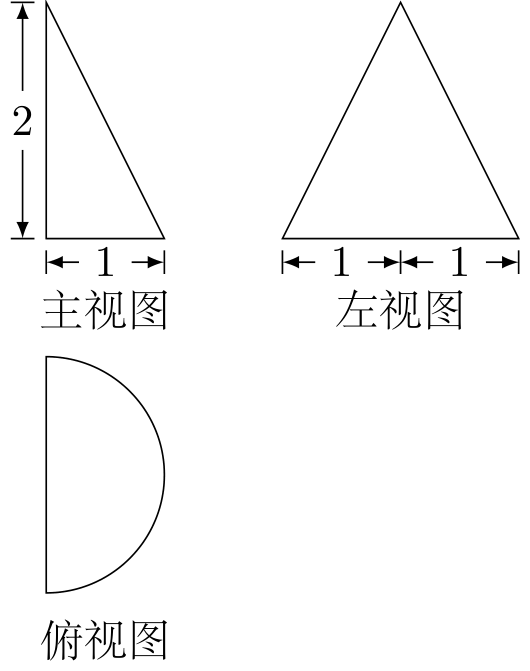
\includegraphics[width=5.1cm]{GaoKao/images/2013/shaanxi_science/q12_fig1.png}
\end{center}

        \item 若点 \((x,y)\) 位于曲线 \(y=\left|x-1\right|\) 与 \(y=2\) 所围成的封闭区域，则 \(2x-y\) 的最小值为\rule[-0.3ex]{3em}{0.4pt}.

        \item 观察下列等式：\(1^2=1\)；\(1^2-2^2=-3\)；\(1^2-2^2+3^2=6\)；\(1^2-2^2+3^2-4^2=-10\). 照此规律，第 \(n\) 个等式可为\rule[-0.3ex]{3em}{0.4pt}.

    \end{enumerate}

\end{description}

\begin{description}

    \item[三、选做题]

    \begin{enumerate}[leftmargin=5pt]

      \addtocounter{enumi}{+14}

        \item 已知 \(a\)，\(b\)，\(m\)，\(n\) 均为正数，且 \(a+b=1\)，\(mn=2\)，则 \((am+bn)(bm+an)\) 的最小值为\rule[-0.3ex]{3em}{0.4pt}.

        \item 如图，弦 \(AB\) 与 \(CD\) 相交于 \(\odot O\) 内一点 \(E\)，过 \(E\) 作 \(BC\) 的平行线与 \(AD\) 的延长线相交于点 \(P\). 已知 \(PD=2DA=2\)，则 \(PE=\rule[-0.3ex]{3em}{0.4pt}\).

\begin{center}
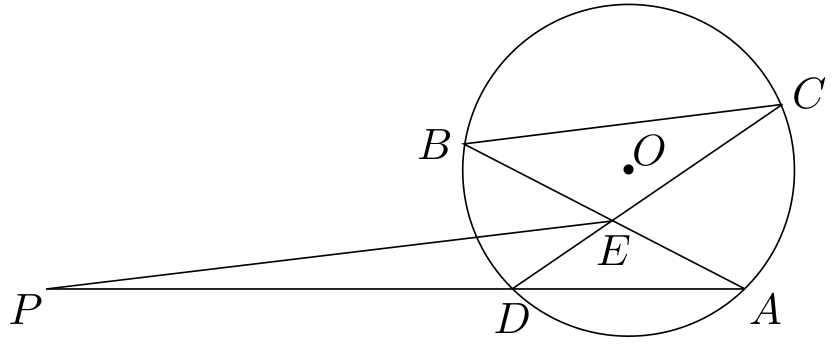
\includegraphics[width=3.8cm]{GaoKao/images/2013/shaanxi_science/q16_fig1.png}
\end{center}

        \item \textbf{【选修4-4：坐标系与参数方程】}

如图，以过原点的直线的倾斜角 \(\theta\) 为参数，则圆 \(x^2+y^2-x=0\) 的参数方程为\rule[-0.3ex]{3em}{0.4pt}.

\begin{center}
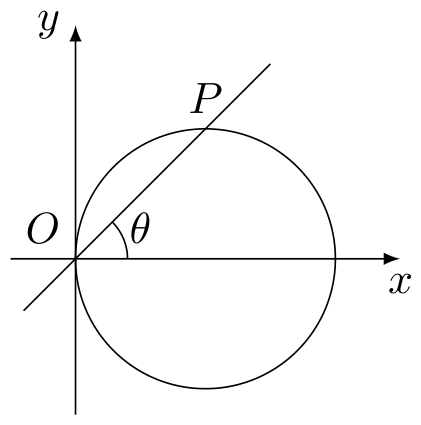
\includegraphics[width=5.2cm]{GaoKao/images/2013/shaanxi_science/q17_fig1.png}
\end{center}

    \end{enumerate}

\end{description}

\begin{description}

    \item[四、解答题]

    \begin{enumerate}[leftmargin=5pt]

      \addtocounter{enumi}{+17}

        \item 已知向量 \(\bm{a}=\left(\cos x,-\dfrac12\right)\)，\(\bm{b}=\left(\sqrt3\sin x,\cos2x\right)\)，\(x\in\mathbb{R}\)，设函数 \(f(x)=\bm{a}\cdot\bm{b}\).

\begin{enumerate}
\item 求 \(f(x)\) 的最小正周期.
\item 求 \(f(x)\) 在 \(\left[0,\dfrac\pi2\right]\) 上的最大值和最小值.
\end{enumerate}

        \item 设 \(\{a_n\}\) 是公比为 \(q\) 的等比数列.

\begin{enumerate}
\item 推导 \(\{a_n\}\) 的前 \(n\) 项和公式；
\item 设 \(q\neq1\)，证明数列 \(\{a_n+1\}\) 不是等比数列.
\end{enumerate}

        \item 如图，四棱柱 \(ABCD-A_{1}B_{1}C_{1}D_{1}\) 的底面 \(ABCD\) 是正方形，\(O\) 为底面中心，\(A_{1}O\perp\) 平面 \(ABCD\)，\(AB=AA_{1}=\sqrt2\).

\begin{enumerate}
\item 证明：\(A_{1}C\perp\) 平面 \(BB_{1}D_{1}D\).
\item 求平面 \(OCB_{1}\) 与平面 \(BB_{1}D_{1}D\) 的夹角 \(\theta\) 的大小.
\end{enumerate}

\begin{center}
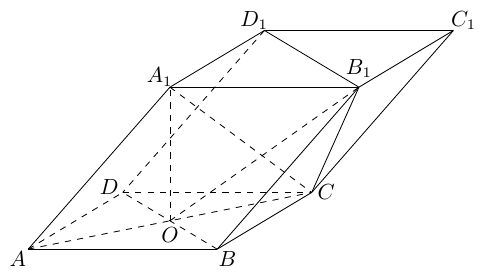
\includegraphics[width=9.9cm]{GaoKao/images/2013/shaanxi_science/q20_fig1.png}
\end{center}

        \item 在一场娱乐晚会上，有 \(5\) 位民间歌手（\(1\) 至 \(5\) 号）登台演唱. 由现场数百名观众投票选出最受欢迎歌手. 各位观众须彼此独立地在选票上选 \(3\) 名歌手，其中观众甲是 \(1\) 号歌手的歌迷，他必选 \(1\) 号，不选 \(2\) 号，另在 \(3\) 至 \(5\) 号中随机选 \(2\) 名. 观众乙和丙对 \(5\) 位歌手的演唱没有偏爱，因此在 \(1\) 至 \(5\) 号中随机选 \(3\) 名歌手.

\begin{enumerate}
\item 求观众甲选中 \(3\) 号歌手且观众乙未选中 \(3\) 号歌手的概率；
\item \(X\) 表示 \(3\) 号歌手得到观众甲、乙、丙的票数之和，求 \(X\) 的分布列和数学期望.
\end{enumerate}

        \item 已知动圆过定点 \(A(4,0)\)，且在 \(y\) 轴上截得的弦 \(MN\) 的长为 \(8\).

\begin{enumerate}
\item 求动圆圆心的轨迹 \(C\) 的方程；
\item 已知点 \(B(-1,0)\)，设不垂直于 \(x\) 轴的直线 \(l\) 与轨迹 \(C\) 交于不同的两点 \(P\)，\(Q\)，若 \(x\) 轴是 \(\angle PBQ\) 的角平分线，证明直线 \(l\) 过定点.
\end{enumerate}

        \item 已知函数 \(f(x)={\mathrm{e}}^x\)，\(x\in\mathbb{R}\).

\begin{enumerate}
\item 若直线 \(y=kx+1\) 与 \(f(x)\) 的反函数的图象相切，求实数 \(k\) 的值；
\item 设 \(x>0\)，讨论曲线 \(y=f(x)\) 与曲线 \(y=mx^2\)（\(m>0\)）公共点的个数；
\item 设 \(a<b\)，比较 \(\dfrac{f(a)+f(b)}{2}\) 与 \(\dfrac{f(b)-f(a)}{b-a}\) 的大小，并说明理由.
\end{enumerate}

    \end{enumerate}

\end{description}


\subsection{2013年陕西卷（文）}\label{gk:2013年陕西卷（文）}

\begin{description}

    \item[一、选择题]

    \begin{enumerate}[leftmargin=5pt]

        \item 设全集为 \(\mathbb{R}\)，函数 \(f(x) = \sqrt{1 - x}\) 的定义域为 \(M\)，则 \(\complement_{\mathbb{R}} M\) 为（\quad）

        {\centering\begin{tabular*}{\linewidth}{@{}@{\extracolsep{\fill}}llll@{}}
          \text{A. }\((-\infty, 1)\)  &  \text{B. }\((1, +\infty)\)  &  \text{C. }\((-\infty, 1]\)  &  \text{D. }\([1, +\infty)\)
        \end{tabular*}\par}

        \item 已知向量 \(\bm{a} = (1, m)\)，\(\bm{b} = (m, 2)\)，若 \(\bm{a} \parallel \bm{b}\)，则实数 \(m\) 等于（\quad）

        {\centering\begin{tabular*}{\linewidth}{@{}@{\extracolsep{\fill}}llll@{}}
          \text{A. }\(-\sqrt{2}\)  &  \text{B. }\(\sqrt{2}\)  &  \text{C. }\(-\sqrt{2}\) 或 \(\sqrt{2}\)  &  \text{D. }0
        \end{tabular*}\par}

        \item 设 \(a\)，\(b\)，\(c\) 均为不等于 1 的正实数，则下列等式中恒成立的是（\quad）

        {\centering\begin{tabular*}{\linewidth}{@{}@{\extracolsep{\fill}}llll@{}}
          \text{A. }\(\log_a b \cdot \log_c b = \log_c a\)  &  \text{B. }\(\log_a b \cdot \log_c a = \log_c b\)  &  \text{C. }\(\log_a (bc) = \log_a b \cdot \log_a c\)  &  \text{D. }\(\log_a(b + c) = \log_a b + \log_a c\)
        \end{tabular*}\par}

        \item 根据下列算法语句，当输入 \(x\) 为 60 时，输出 \(y\) 的值为（\quad）

\begin{center}
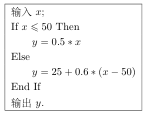
\includegraphics[width=5.4cm]{GaoKao/images/2013/shaanxi_liberal/q4_fig1.png}
\end{center}

        {\centering\begin{tabular*}{\linewidth}{@{}@{\extracolsep{\fill}}llll@{}}
          \text{A. }25  &  \text{B. }30  &  \text{C. }31  &  \text{D. }61
        \end{tabular*}\par}

        \item 对一批产品的长度（单位：毫米）进行抽样检测，下图为检测结果的频率分布直方图，根据标准，产品长度在区间 \([20, 25)\) 上为一等品，在区间 \([15, 20)\) 和 \([25, 30)\) 上为二等品，在区间 \([10, 15)\) 和 \([30, 35]\) 上为三等品. 用频率估计概率，现从该批产品中随机抽取 1 件，则其为二等品的概率是（\quad）

\begin{center}
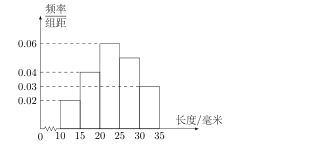
\includegraphics[width=0.55\linewidth]{GaoKao/images/2013/shaanxi_liberal/q5_fig1.png}
\end{center}

        {\centering\begin{tabular*}{\linewidth}{@{}@{\extracolsep{\fill}}llll@{}}
          \text{A. }0.09  &  \text{B. }0.20  &  \text{C. }0.25  &  \text{D. }0.45
        \end{tabular*}\par}

        \item 设 \(z\) 是复数，则下列命题中的假命题是（\quad）

        {\centering\begin{tabular*}{\linewidth}{@{}@{\extracolsep{\fill}}llll@{}}
          \text{A. }若 \( z^{2} \geqslant 0 \)，则 \(z\) 是实数  &  \text{B. }若 \(z^2 < 0\)，则 \(z\) 是虚数  &  \text{C. }若 \(z\) 是虚数，则 \(z^2 \geqslant 0\)  &  \text{D. }若 \(z\) 是纯虚数，则 \(z^2 < 0\)
        \end{tabular*}\par}

        \item 若点 \((x, y)\) 位于曲线 \(y = |x|\) 与 \(y = 2\) 所围成的封闭区域，则 \(2x - y\) 的最小值是（\quad）

        {\centering\begin{tabular*}{\linewidth}{@{}@{\extracolsep{\fill}}llll@{}}
          \text{A. }\(-6\)  &  \text{B. }\(-2\)  &  \text{C. }0  &  \text{D. }2
        \end{tabular*}\par}

        \item 已知点 \(M(a, b)\) 在圆 \(O: x^2 + y^2 = 1\) 外，则直线 \(ax + by = 1\) 与圆 \(O\) 的位置关系是（\quad）

        {\centering\begin{tabular*}{\linewidth}{@{}@{\extracolsep{\fill}}llll@{}}
          \text{A. }相切  &  \text{B. }相交  &  \text{C. }相离  &  \text{D. }不确定
        \end{tabular*}\par}

        \item 设 \(\triangle ABC\) 的内角 \(A\)，\(B\)，\(C\) 所对的边分别为 \(a\)，\(b\)，\(c\)，若 \(b \cos C + c \cos B = a \sin A\)，则 \(\triangle ABC\) 的形状为（\quad）

        {\centering\begin{tabular*}{\linewidth}{@{}@{\extracolsep{\fill}}llll@{}}
          \text{A. }直角三角形  &  \text{B. }锐角三角形  &  \text{C. }钝角三角形  &  \text{D. }不确定
        \end{tabular*}\par}

        \item 设 \([x]\) 表示不大于 \(x\) 的最大整数，则对任意实数 \(x\)，有（\quad）

        {\centering\begin{tabular*}{\linewidth}{@{}@{\extracolsep{\fill}}llll@{}}
          \text{A. }\([-x] = -[x]\)  &  \text{B. }\(\left[x + \frac{1}{2}\right] = [x]\)  &  \text{C. }\([2x] = 2[x]\)  &  \text{D. }\([x] + \left[x + \frac{1}{2}\right] = [2x]\)
        \end{tabular*}\par}

    \end{enumerate}

\end{description}

\begin{description}

    \item[二、填空题]

    \begin{enumerate}[leftmargin=5pt]

      \addtocounter{enumi}{+10}

        \item 双曲线 \( \frac{x^{2}}{16}-\frac{y^{2}}{9}=1 \) 的离心率为\rule[-0.3ex]{3em}{0.4pt}.

        \item 某几何体的三视图如图所示，则其表面积为\rule[-0.3ex]{3em}{0.4pt}.

\begin{center}
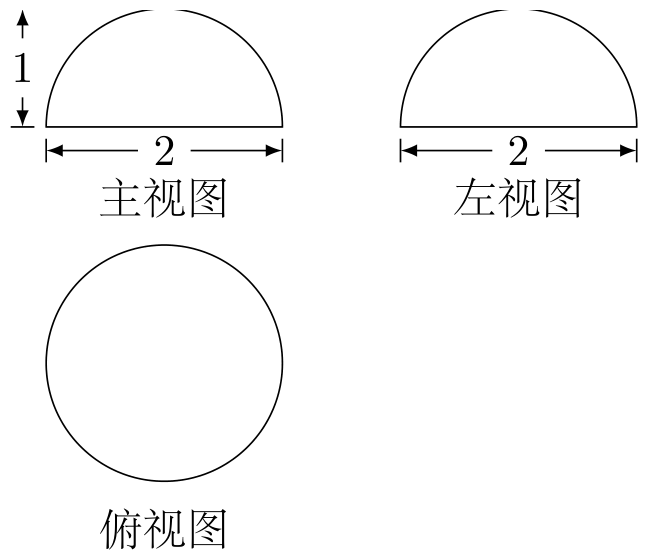
\includegraphics[width=6.3cm]{GaoKao/images/2013/shaanxi_liberal/q12_fig1.png}
\end{center}

        \item 观察下列等式：\(1 + 1 = 2 \times 1\)，\((2 + 1)(2 + 2) = 2^{2} \times 1 \times 3\)，\((3 + 1)(3 + 2)(3 + 3) = 2^{3} \times 1 \times 3 \times 5\).

照此规律，第 \(n\) 个等式可为\rule[-0.3ex]{3em}{0.4pt}.

        \item 在如图所示的锐角三角形空地中，欲建一个面积最大的内接矩形花园（阴影部分），则其边长 \(x\) 为\rule[-0.3ex]{3em}{0.4pt}\(\mathrm{m}\).
\begin{center}
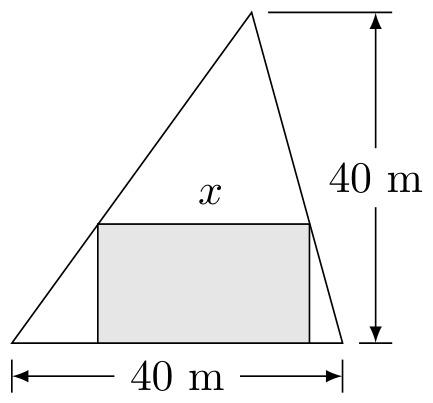
\includegraphics[width=4.1cm]{GaoKao/images/2013/shaanxi_liberal/q14_fig1.png}
\end{center}

    \end{enumerate}

\end{description}

\begin{description}

    \item[三、选考题]

    \begin{enumerate}[leftmargin=5pt]

      \addtocounter{enumi}{+14}

        \item \textbf{【选修4-5：不等式选讲】}

设 \(a,b \in \mathbb{R}\)，\(|a - b| > 2\)，则关于实数 \(x\) 的不等式 \(|x - a| + |x - b| > 2\) 的解集是\rule[-0.3ex]{3em}{0.4pt}.

        \item 如图，\(AB\) 与 \(CD\) 相交于点 \(E\)，过 \(E\) 作 \(BC\) 的平行线与 \(AD\) 的延长线交于点 \(P\)，已知 \(\angle A = \angle C\)，\(PD = 2DA = 2\)，则 \(PE =\rule[-0.3ex]{3em}{0.4pt}\).
\begin{center}
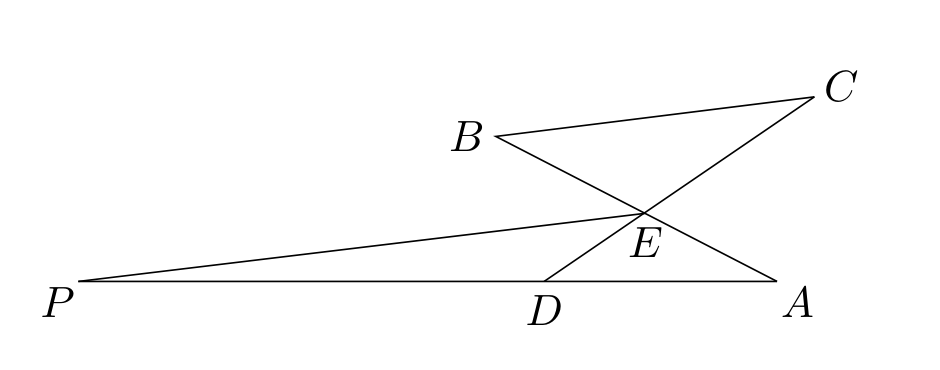
\includegraphics[width=9.0cm]{GaoKao/images/2013/shaanxi_liberal/q16_fig1.png}
\end{center}

        \item \textbf{【选修4-1：几何证明选讲】}

圆锥曲线 \(x = t^{2}\)，\(\ y = 2t\)（\(t\) 为参数）的焦点坐标是\rule[-0.3ex]{3em}{0.4pt}.

    \end{enumerate}

\end{description}

\begin{description}

    \item[四、解答题]

    \begin{enumerate}[leftmargin=5pt]

      \addtocounter{enumi}{+17}

        \item 已知向量 \(\bm{a} = \left(\cos x, -\frac{1}{2}\right)\)，\(\bm{b} = (\sqrt{3} \sin x, \cos 2x)\)，\(x \in \mathbb{R}\)，设函数 \(f(x) = \bm{a} \cdot \bm{b}\).

\begin{enumerate}
\item 求 \( f(x) \) 的最小正周期.
\item 求 \( f(x) \) 在 \( \left[0, \frac{\pi}{2}\right] \) 上的最大值和最小值.
\end{enumerate}

        \item 设 \(S_{n}\) 表示数列 \(\{a_{n}\}\) 的前 \(n\) 项和.

\begin{enumerate}
\item 若 \( \{a_{n}\} \) 是等差数列，推导 \( S_{n} \) 的计算公式.
\item 若 \(a_{1} = 1\)，\(q \neq 0\)，且对所有正整数 \(n\)，有 \(S_{n} = \frac{1 - q^{n}}{1 - q}\)，判断 \(\{a_{n}\}\) 是否为等比数列，并证明你的结论.
\end{enumerate}

        \item 如图，四棱柱 \(ABCD - A_{1}B_{1}C_{1}D_{1}\) 的底面 \(ABCD\) 是正方形，\(O\) 为底面中心，\(A_{1}O \perp\) 平面 \(ABCD\)，\(AB = AA_{1} = \sqrt{2}\).

\begin{enumerate}
\item 证明：平面 \(A_{1}BD\) \(\parallel\) 平面 \(CD_{1}B_{1}\).
\item 求三棱柱 \( ABD - A_{1}B_{1}D_{1} \) 的体积.
\end{enumerate}

\begin{center}
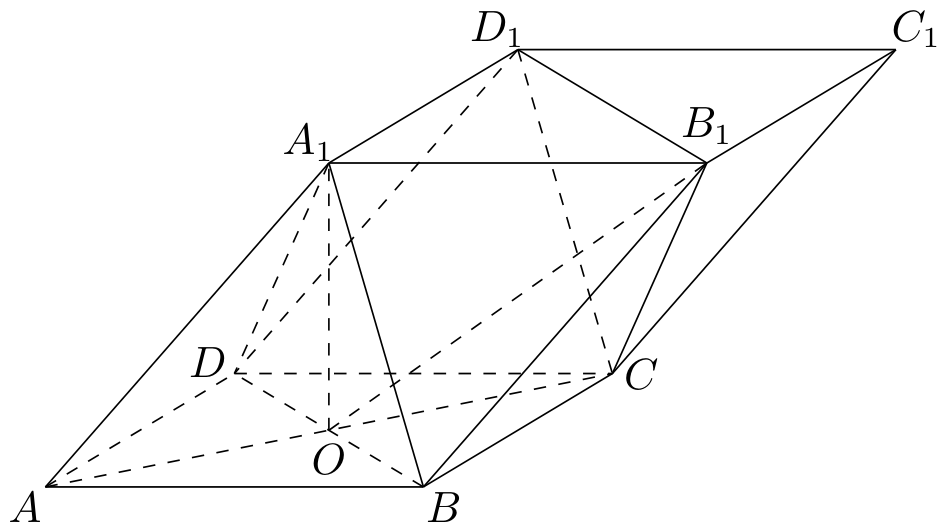
\includegraphics[width=9.9cm]{GaoKao/images/2013/shaanxi_liberal/q20_fig1.png}
\end{center}

        \item 有 7 位歌手（1至7号）参加一场歌唱比赛，由 500 名大众评委现场投票决定歌手名次. 根据年龄将大众评委分为五组，各组的人数如下：

\begin{center}
\begingroup
\small
\renewcommand{\arraystretch}{1.2}
\begin{tabular}{|c|c|c|c|c|c|}
\hline
组别 & A & B & C & D & E \\
\hline
人数 & 50 & 100 & 150 & 150 & 50 \\
\hline
\end{tabular}
\endgroup
\end{center}

\begin{enumerate}
\item 为了调查评委对 7 位歌手的支持情况，现用分层抽样方法从各组中抽取若干评委，其中从 B 组抽取了 6 人，请将其余各组抽取的人数填入下表.

\begin{center}
\begingroup
\small
\renewcommand{\arraystretch}{1.2}
\begin{tabular}{|c|c|c|c|c|c|}
\hline
组别 & A & B & C & D & E \\
\hline
人数 & 50 & 100 & 150 & 150 & 50 \\
\hline
抽取人数 &  & 6 &  &  &  \\
\hline
\end{tabular}
\endgroup
\end{center}

\item 在上一问中，若 \(A\)，\(B\) 两组被抽到的评委中各有 2 人支持 1 号歌手，现从这两组被抽到的评委中分别任选 1 人，求这 2 人都支持 1 号歌手的概率.
\end{enumerate}

        \item 已知动点 \(M(x, y)\) 到直线 \(l: x = 4\) 的距离是它到点 \(N(1,0)\) 的距离的2倍.

\begin{enumerate}
\item 求动点 \(M\) 的轨迹 \(C\) 的方程.
\item 过点 \(P(0,3)\) 的直线 \(m\) 与轨迹 \(C\) 交于 \(A\)，\(B\) 两点，若 \(A\) 是 \(PB\) 的中点，求直线 \(m\) 的斜率.
\end{enumerate}

        \item 已知函数 \(f(x) = {\mathrm{e}}^{x}\)，\(x \in \mathbb{R}\).

\begin{enumerate}
\item 求 \( f(x) \) 的反函数的图象上点 \((1,0)\) 处的切线方程.
\item 证明：曲线 \( y = f(x) \) 与曲线 \( y = \frac{1}{2} x^2 + x + 1 \) 有唯一公共点.
\item 设 \(a < b\)，比较 \(f\left(\frac{a + b}{2}\right)\) 与 \(\frac{f(b) - f(a)}{b - a}\) 的大小，并说明理由.
\end{enumerate}

    \end{enumerate}

\end{description}


\subsection{2013年天津卷（理）}\label{gk:2013年天津卷（理）}

\begin{description}

    \item[一、选择题]

    \begin{enumerate}[leftmargin=5pt]

        \item 已知集合 \(A = \{x \in \mathbb{R} \mid |x| \leqslant 2\}\)，\(B = \{x \in \mathbb{R} \mid x \leqslant 1\}\)，则 \(A \cap B =\)（\quad）

        {\centering\begin{tabular*}{\linewidth}{@{}@{\extracolsep{\fill}}llll@{}}
          \text{A. }\((-\infty, 2]\)  &  \text{B. }\([1,2]\)  &  \text{C. }\([-2, 2]\)  &  \text{D. }\([-2, 1]\)
        \end{tabular*}\par}

        \item 设变量 \(x\)，\(y\) 满足约束条件 \(\begin{cases}
3x + y - 6 \geqslant 0,\\
x - y - 2 \leqslant 0,\\
y - 3 \leqslant 0,
\end{cases}\) 则目标函数 \(z = y - 2x\) 的最小值为（\quad）

        {\centering\begin{tabular*}{\linewidth}{@{}@{\extracolsep{\fill}}llll@{}}
          \text{A. }\(-7\)  &  \text{B. }\(-4\)  &  \text{C. }1  &  \text{D. }2
        \end{tabular*}\par}

        \item 阅读如图的程序框图，运行相应的程序，若输入 \(x\) 的值为 1，则输出 \(S\) 的值为（\quad）

\begin{center}
\includegraphics[width=0.46\linewidth]{GaoKao/images/2013/tianjin_science/q3_fig1.png}
\end{center}

        {\centering\begin{tabular*}{\linewidth}{@{}@{\extracolsep{\fill}}llll@{}}
          \text{A. }64  &  \text{B. }73  &  \text{C. }512  &  \text{D. }585
        \end{tabular*}\par}

        \item 已知下列三个命题：

\begin{enumerate}
\item 若一个球的半径缩小到原来的 \(\frac{1}{2}\)，则其体积缩小到原来的 \(\frac{1}{8}\)；
\item 若两组数据的平均数相等，则它们的标准差也相等；
\item 直线 \(x + y + 1 = 0\) 与圆 \(x^{2} + y^{2} = \frac{1}{2}\) 相切.
\end{enumerate}

其中真命题的序号是（\quad）

        {\centering\begin{tabular*}{\linewidth}{@{}@{\extracolsep{\fill}}llll@{}}
          \text{A. }\ding{172}\ding{173}\ding{174}  &  \text{B. }\ding{172}\ding{173}  &  \text{C. }\ding{172}\ding{174}  &  \text{D. }\ding{173}\ding{174}
        \end{tabular*}\par}

        \item 已知双曲线 \(\frac{x^2}{a^2} - \frac{y^2}{b^2} = 1 \) （\(a > 0, b > 0\)）的两条渐近线与抛物线 \(y^2 = 2px\) （\(p > 0\)）的准线分别交于 \(A\)，\(B\) 两点，\(O\) 为坐标原点. 若双曲线的离心率为 2，\(\triangle AOB\) 的面积为 \(\sqrt{3}\)，则 \(p =\)（\quad）

        {\centering\begin{tabular*}{\linewidth}{@{}@{\extracolsep{\fill}}llll@{}}
          \text{A. }1  &  \text{B. }\(\frac{3}{2}\)  &  \text{C. }2  &  \text{D. }3
        \end{tabular*}\par}

        \item 在 \(\triangle ABC\) 中，\(\angle ABC = \frac{\pi}{4}\)，\(AB = \sqrt{2}\)，\(BC = 3\). 则 \(\sin \angle BAC =\)（\quad）

        {\centering\begin{tabular*}{\linewidth}{@{}@{\extracolsep{\fill}}llll@{}}
          \text{A. }\(\frac{\sqrt{10}}{10}\)  &  \text{B. }\(\frac{\sqrt{10}}{5}\)  &  \text{C. }\(\frac{3\sqrt{10}}{10}\)  &  \text{D. }\(\frac{\sqrt{5}}{5}\)
        \end{tabular*}\par}

        \item 函数 \( f(x) = 2^{x} |\log_{0.5} x| - 1 \) 的零点个数为（\quad）

        {\centering\begin{tabular*}{\linewidth}{@{}@{\extracolsep{\fill}}llll@{}}
          \text{A. }1  &  \text{B. }2  &  \text{C. }3  &  \text{D. }4
        \end{tabular*}\par}

        \item 已知函数 \( f(x) = x(1 + a|x|) \). 设关于 \( x \) 的不等式 \( f(x + a) < f(x) \) 的解集为 \(A\). 若 \( \left[-\frac{1}{2}, \frac{1}{2}\right] \subseteq A \)，则实数 \( a \) 的取值范围是（\quad）

        {\centering\begin{tabular*}{\linewidth}{@{}@{\extracolsep{\fill}}llll@{}}
          \text{A. }\(\left(\frac{1 - \sqrt{5}}{2}, 0\right)\)  &  \text{B. }\(\left(\frac{1 - \sqrt{3}}{2}, 0\right)\)  &  \text{C. }\(\left(\frac{1 - \sqrt{5}}{2}, 0\right) \cup \left(0, \frac{1 + \sqrt{3}}{2}\right)\)  &  \text{D. }\(\left(-\infty, \frac{1 - \sqrt{5}}{2}\right)\)
        \end{tabular*}\par}

    \end{enumerate}

\end{description}

\begin{description}

    \item[二、填空题]

    \begin{enumerate}[leftmargin=5pt]

      \addtocounter{enumi}{+8}

        \item 已知 \(a\)，\(b \in \mathbb{R}\)，\(\i\) 是虚数单位. 若 \((a + \i)(1 + \i) = b\i\)，则 \(a + b\i =\rule[-0.3ex]{3em}{0.4pt}\).

        \item \(\left(x - \frac{1}{\sqrt{x}}\right)^6\) 的二项展开式中的常数项为\rule[-0.3ex]{3em}{0.4pt}.

        \item 已知圆的极坐标方程为 \(\rho = 4\cos \theta\)，圆心为 \(C\)，点 \(P\) 的极坐标为 \(\left(4, \frac{\pi}{3}\right)\)，则 \(|CP| = \)\rule[-0.3ex]{3em}{0.4pt}.

        \item 在平行四边形 \(ABCD\) 中，\(AD = 1\)，\(\angle BAD = 60^{\circ}\)，\(E\) 为 \(CD\) 的中点. 若 \(\overrightarrow{AC} \cdot \overrightarrow{BE} = 1\)，则 \(AB\) 的长为\rule[-0.3ex]{3em}{0.4pt}.

        \item 如图，\(\triangle ABC\) 为圆的内接三角形，\(BD\) 为圆的弦，且 \(BD \parallel AC\). 过点 \(A\) 作圆的切线与 \(DB\) 的延长线交于点 \(E\)，\(AD\) 与 \(BC\) 交于点 \(F\). 若 \(AB = AC\)，\(AE = 6\)，\(BD = 5\)，则线段 \(CF\) 的长为\rule[-0.3ex]{3em}{0.4pt}.
\begin{center}
\includegraphics[width=8.1cm]{GaoKao/images/2013/tianjin_science/q13_fig1.png}
\end{center}

        \item 设 \(a + b = 2\)，\(b > 0\)，则当 \(a =\rule[-0.3ex]{3em}{0.4pt}\) 时，\(\frac{1}{2|a|} + \frac{|a|}{b}\) 取得最小值.

    \end{enumerate}

\end{description}

\begin{description}

    \item[三、解答题]

    \begin{enumerate}[leftmargin=5pt]

      \addtocounter{enumi}{+14}

        \item 已知函数 \(f(x) = -\sqrt{2} \sin \left(2x + \frac{\pi}{4}\right) + 6 \sin x \cos x - 2 \cos^2 x + 1\)，\(x \in \mathbb{R}\).
\begin{enumerate}
\item 求 \( f(x) \) 的最小正周期；
\item 求 \( f(x) \) 在区间 \([0, \frac{\pi}{2}]\) 上的最大值和最小值.
\end{enumerate}

        \item 一个盒子里装有7张卡片，其中有红色卡片4张，编号分别为1， 2， 3， 4；白色卡片3张，编号分别为2， 3， 4. 从盒子中任取4张卡片（假设取到任何一张卡片的可能性相同）.
\begin{enumerate}
\item 求取出的 4 张卡片中，含有编号为 3 的卡片的概率.
\item 在取出的 4 张卡片中，红色卡片编号的最大值设为 \(X\)，求随机变量 \(X\) 的分布列和数学期望.
\end{enumerate}

        \item 如图所示，在四棱柱 \(ABCD - A_{1}B_{1}C_{1}D_{1}\) 中，侧棱 \(A_{1}A \perp\) 底面 \(ABCD\)，\(AB \parallel DC\)，\(AB \perp AD\)，\(AD = CD = 1\)，\(AA_{1} = AB = 2\)，\(E\) 为棱 \(AA_{1}\) 的中点.
\begin{enumerate}
\item 证明： \( B_{1}C_{1}\perp CE \)；
\item 求二面角 \(B_{1} - CE - C_{1}\) 的平面角的正弦值；
\item 设点 \(M\) 在线段 \(C_{1}E\) 上，且直线 \(AM\) 与平面 \(ADD_{1}A_{1}\) 所成角的正弦值为 \( \frac{\sqrt{2}}{6} \)，求线段 \(AM\) 的长.
\end{enumerate}
\begin{center}
\includegraphics[width=6.2cm]{GaoKao/images/2013/tianjin_science/q17_fig1.png}
\end{center}

        \item 设椭圆 \(\frac{x^2}{a^2} + \frac{y^2}{b^2} = 1 \) （\(a > b > 0\)）的左焦点为 \(F\)，离心率为 \(\frac{\sqrt{3}}{3}\)，过点 \(F\) 且与 \(x\) 轴垂直的直线被椭圆截得的线段长为 \(\frac{4\sqrt{3}}{3}\).
\begin{enumerate}
\item 求椭圆的方程；
\item 设 \(A\)，\(B\) 分别为椭圆的左，右顶点，过点 \(F\) 且斜率为 \(k\) 的直线与椭圆交于 \(C\)，\(D\) 两点. 若 \(\overrightarrow{AC} \cdot \overrightarrow{DB} + \overrightarrow{AD} \cdot \overrightarrow{CB} = 8\)，求 \(k\) 的值.
\end{enumerate}

        \item 已知首项为 \(\frac{3}{2}\) 的等比数列 \(\{a_{n}\}\) 不是递减数列. 其前 \(n\) 项和为 \(S_{n}\) （\(n \in \mathbf{N}^{*}\)），且 \(S_{3} + a_{3}\)，\(S_{5} + a_{5}\)，\(S_{4} + a_{4}\) 成等差数列.
\begin{enumerate}
\item 求数列 \( \{a_{n}\} \) 的通项公式；
\item 设 \(T_{n} = S_{n} - \frac{1}{S_{n}}\) （\(n \in \mathbf{N}^{*}\)），求数列 \(\{T_{n}\}\) 的最大项的值与最小项的值.
\end{enumerate}

        \item 已知函数 \( f(x) = x^2 \ln x \).
\begin{enumerate}
\item 求函数 \( f(x) \) 的单调区间；
\item 证明：对任意的 \(t > 0\)，存在唯一的 \(s\)，使 \(t = f(s)\).
\item 设（2）中所确定的 \(s\) 关于 \(t\) 的函数为 \(s = g(t)\)，证明：当 \(t > {\mathrm{e}}^2\) 时，有 \( \frac {2}{5} < \frac {\ln g(t)}{\ln t} < \frac {1}{2} \).
\end{enumerate}

    \end{enumerate}

\end{description}


\subsection{2013年天津卷（文）}\label{gk:2013年天津卷（文）}

\begin{description}

    \item[一、选择题]

    \begin{enumerate}[leftmargin=5pt]

        \item 已知集合 \(A = \{x \in \mathbb{R} \mid |x| \leqslant 2\}\)，\(B = \{x \in \mathbb{R} \mid x \leqslant 1\}\)，则 \(A \cap B =\)（\quad）

        {\centering\begin{tabular*}{\linewidth}{@{}@{\extracolsep{\fill}}llll@{}}
          \text{A. }\((-\infty, 2]\)  &  \text{B. }\([1,2]\)  &  \text{C. }\([-2, 2]\)  &  \text{D. }\([-2, 1]\)
        \end{tabular*}\par}

        \item 设变量 \(x\)，\(y\) 满足约束条件 \(\begin{cases}
3x + y - 6 \geqslant 0,\\
x - y - 2 \leqslant 0,\\
y - 3 \leqslant 0,
\end{cases}\) 则目标函数 \(z = y - 2x\) 的最小值为（\quad）

        {\centering\begin{tabular*}{\linewidth}{@{}@{\extracolsep{\fill}}llll@{}}
          \text{A. }\(-7\)  &  \text{B. }\(-4\)  &  \text{C. }1  &  \text{D. }2
        \end{tabular*}\par}

        \item 阅读如图所示的程序框图，运行相应的程序，则输出 \(n\) 的值为（\quad）

\begin{center}
\includegraphics[width=0.42\linewidth]{GaoKao/images/2013/tianjin_liberal/q3_fig1.png}
\end{center}

        {\centering\begin{tabular*}{\linewidth}{@{}@{\extracolsep{\fill}}llll@{}}
          \text{A. }7  &  \text{B. }6  &  \text{C. }5  &  \text{D. }4
        \end{tabular*}\par}

        \item 设 \(a\)，\(b \in \mathbb{R}\)，则“\((a - b) \cdot a^2 < 0\)”是“\(a < b\)”的（\quad）

        {\centering\begin{tabular*}{\linewidth}{@{}@{\extracolsep{\fill}}llll@{}}
          \text{A. }充分而不必要条件  &  \text{B. }必要而不充分条件  &  \text{C. }充要条件  &  \text{D. }既不充分也不必要条件
        \end{tabular*}\par}

        \item 已知过点 \(P(2,2)\) 的直线与 \((x - 1)^2 + y^2 = 5\) 相切，且与直线 \(ax - y + 1 = 0\) 垂直，则 \(a =\)（\quad）

        {\centering\begin{tabular*}{\linewidth}{@{}@{\extracolsep{\fill}}llll@{}}
          \text{A. }\(-\frac{1}{2}\)  &  \text{B. }1  &  \text{C. }2  &  \text{D. }\(\frac{1}{2}\)
        \end{tabular*}\par}

        \item 函数 \( f(x) = \sin \left(2x - \frac{\pi}{4}\right) \) 在区间 \(\left[0, \frac{\pi}{2}\right]\) 上的最小值为（\quad）

        {\centering\begin{tabular*}{\linewidth}{@{}@{\extracolsep{\fill}}llll@{}}
          \text{A. }\(-1\)  &  \text{B. }\(-\frac{\sqrt{2}}{2}\)  &  \text{C. }\(\frac{\sqrt{2}}{2}\)  &  \text{D. }0
        \end{tabular*}\par}

        \item 已知函数 \( f(x) \) 是定义在 \( \mathbb{R} \) 上的偶函数，且在区间 \( [0, +\infty) \) 上单调递增. 若实数 \( a \) 满足 \( f(\log_{2} a) + f(\log_{\frac{1}{2}} a) \leqslant 2f(1) \)，则 \( a \) 的取值范围是（\quad）

        {\centering\begin{tabular*}{\linewidth}{@{}@{\extracolsep{\fill}}llll@{}}
          \text{A. }\([1,2]\)  &  \text{B. }\(\left(0, \frac{1}{2}\right]\)  &  \text{C. }\(\left[\frac{1}{2}, 2\right]\)  &  \text{D. }\((0,2]\)
        \end{tabular*}\par}

        \item 设函数 \( f(x) = {\mathrm{e}}^{x} + x - 2 \)，\( g(x) = \ln x + x^2 - 3 \). 若实数 \(a\)，\(b\) 满足 \( f(a) = 0 \)，\( g(b) = 0 \)，则（\quad）

        {\centering\begin{tabular*}{\linewidth}{@{}@{\extracolsep{\fill}}llll@{}}
          \text{A. }\(g(a) < 0 < f(b)\)  &  \text{B. }\(f(b) < 0 < g(a)\)  &  \text{C. }\(0 < g(a) < f(b)\)  &  \text{D. }\(f(b) < g(a) < 0\)
        \end{tabular*}\par}

    \end{enumerate}

\end{description}

\begin{description}

    \item[二、填空题]

    \begin{enumerate}[leftmargin=5pt]

      \addtocounter{enumi}{+8}

        \item \(\i\) 是虚数单位，复数 \( (3+\i)(1-2\i)= \)\rule[-0.3ex]{3em}{0.4pt}.

        \item 已知一个正方体的所有顶点在一个球面上，若球的体积为 \(\frac{9\pi}{2}\)，则正方体的棱长为\rule[-0.3ex]{3em}{0.4pt}.

        \item 已知抛物线 \( y^{2} = 8x \) 的准线过双曲线 \( \frac{x^2}{a^2} - \frac{y^2}{b^2} = 1  \) （\(a > 0, b > 0\)）的一个焦点，且双曲线的离心率为 2，则该双曲线的方程为\rule[-0.3ex]{3em}{0.4pt}.

        \item 在平行四边形 \(ABCD\) 中，\(AD = 1\)，\(\angle BAD = 60^{\circ}\)，\(E\) 为 \(CD\) 的中点. 若 \(\overrightarrow{AC} \cdot \overrightarrow{BE} = 1\)，则 \(AB\) 的长为\rule[-0.3ex]{3em}{0.4pt}.

        \item 如图，在圆内接梯形 \(ABCD\) 中，\(AB \parallel DC\)，过点 \(A\) 作圆的切线与 \(CB\) 的延长线交于点 \(E\). 若 \(AB = AD = 5\)，\(BE = 4\)，则弦 \(BD\) 的长为\rule[-0.3ex]{3em}{0.4pt}.

\begin{center}
\includegraphics[width=7.2cm]{GaoKao/images/2013/tianjin_liberal/q13_fig1.png}
\end{center}

        \item 设 \(a + b = 2\)，\(b > 0\)，则 \(\frac{1}{2|a|} + \frac{|a|}{b}\) 的最小值为\rule[-0.3ex]{3em}{0.4pt}.

    \end{enumerate}

\end{description}

\begin{description}

    \item[三、解答题]

    \begin{enumerate}[leftmargin=5pt]

      \addtocounter{enumi}{+14}

        \item 某产品的三个质量指标分别为 \(x\)，\(y\)，\(z\)，用综合指标 \(S = x + y + z\) 评价该产品的等级. 若 \(S \leqslant 4\)，则该产品为一等品. 现从一批该产品中，随机抽取 \(10\) 件产品作为样本，其质量指标列表如下：

\begin{center}
\begingroup
\small
\renewcommand{\arraystretch}{1.2}
\begin{tabular}{|c|c|c|c|c|c|}
\hline
产品编号 & \(A_1\) & \(A_2\) & \(A_3\) & \(A_4\) & \(A_5\) \\
\hline
质量指标 \((x,y,z)\) & \((1,1,2)\) & \((2,1,1)\) & \((2,2,2)\) & \((1,1,1)\) & \((1,2,1)\) \\
\hline
产品编号 & \(A_6\) & \(A_7\) & \(A_8\) & \(A_9\) & \(A_{10}\) \\
\hline
质量指标 \((x,y,z)\) & \((1,2,2)\) & \((2,1,1)\) & \((2,2,1)\) & \((1,1,1)\) & \((2,1,2)\) \\
\hline
\end{tabular}
\endgroup
\end{center}

\begin{enumerate}
\item 利用上表提供的样本数据估计出该批产品的一等品率；
\item 在该样本的一等品中，随机抽取 \(2\) 件产品.
\begin{enumerate}
\item 用产品编号列出所有可能的结果；
\item 设事件 \(B\) 为“在取出的 \(2\) 件产品中，每件产品的综合指标 \(S\) 都等于 \(4\)”，求事件 \(B\) 发生的概率.
\end{enumerate}
\end{enumerate}

        \item 在 \(\triangle ABC\) 中，内角 \(A\)，\(B\)，\(C\) 所对的边分别是 \(a\)，\(b\)，\(c\)，已知 \(b \sin A = 3c \sin B\)，\(a = 3\)，\(\cos B = \frac{2}{3}\).
\begin{enumerate}
\item 求 \(b\) 的值；
\item 求 \( \sin\left(2B-\frac{\pi}{3}\right) \) 的值.
\end{enumerate}

        \item 如图，三棱柱 \(ABC - A_{1}B_{1}C_{1}\) 中，侧棱 \(A_{1}A \perp\) 底面 \(ABC\)，且各棱长均相等，\(D\)，\(E\)，\(F\) 分别为棱 \(AB\)，\(BC\)，\(A_{1}C_{1}\) 的中点.
\begin{enumerate}
\item 证明 \(EF \parallel\) 平面 \(A_{1}CD\)；
\item 证明平面 \(A_{1}CD \perp\) 平面 \(A_{1}ABB_{1}\)；
\item 求直线 \(BC\) 与平面 \(A_{1}CD\) 所成角的正弦值.
\end{enumerate}

\begin{center}
\includegraphics[width=7.0cm]{GaoKao/images/2013/tianjin_liberal/q17_fig1.png}
\end{center}

        \item 设椭圆 \(\frac{x^2}{a^2} + \frac{y^2}{b^2} = 1 \) （\(a > b > 0\)）的左焦点为 \(F\)，离心率为 \(\frac{\sqrt{3}}{3}\)，过点 \(F\) 且与 \(x\) 轴垂直的直线被椭圆截得的线段长为 \(\frac{4\sqrt{3}}{3}\).
\begin{enumerate}
\item 求椭圆的方程；
\item 设 \(A\)，\(B\) 分别为椭圆的左，右顶点，过点 \(F\) 且斜率为 \(k\) 的直线与椭圆交于 \(C\)，\(D\) 两点. 若 \(\overrightarrow{AC} \cdot \overrightarrow{DB} + \overrightarrow{AD} \cdot \overrightarrow{CB} = 8\)，求 \(k\) 的值.
\end{enumerate}

        \item 已知首项为 \(\frac{3}{2}\) 的等比数列 \(\{a_{n}\}\) 的前 \(n\) 项和为 \(S_{n}\) （\(n \in \mathbf{N}^{*}\)），且 \(-2S_{2}\)，\(S_{3}\)，\(4S_{4}\) 成等差数列.
\begin{enumerate}
\item 求数列 \( \{a_{n}\} \) 的通项公式；
\item 证明 \(S_{n} + \frac{1}{S_{n}} \leqslant \frac{13}{6} \) （\(n \in \mathbf{N}^{*}\)）.
\end{enumerate}

        \item 设 \(a \in [-2,0]\)，已知函数 \(f(x) = \begin{cases}
x^2 - (a + 5)x, & x \leqslant 0,\\
x^3 - \frac{a + 3}{2}x^2 + ax, & x > 0.
\end{cases}\)
\begin{enumerate}
\item 证明： \( f(x) \) 在区间 \( (-1,1) \) 内单调递减，在区间 \( (1,+\infty) \) 内单调递增；
\item 设曲线 \( y = f(x) \) 在点 \( P_i(x_i, f(x_i)) \) （\(i = 1\)，\(2\)，\(3\)） 处的切线相互平行，且 \( x_{1}x_{2}x_{3} \neq 0 \)，证明：\( x_{1} + x_{2} + x_{3} > -\frac{1}{3} \).
\end{enumerate}

    \end{enumerate}

\end{description}


\subsection{2013年浙江卷（理）}\label{gk:2013年浙江卷（理）}

\begin{description}

    \item[一、选择题]

    \begin{enumerate}[leftmargin=5pt]

        \item 已知 \(\i\) 是虚数单位，则 \((-1 + \i)(2 - \i) =\)（\quad）

        {\centering\begin{tabular*}{\linewidth}{@{}@{\extracolsep{\fill}}llll@{}}
          \text{A. }\(-3 + \i\)  &  \text{B. }\(-1 + 3\i\)  &  \text{C. }\(-3 + 3\i\)  &  \text{D. }\(-1 + \i\)
        \end{tabular*}\par}

        \item 设集合 \(S = \{x \mid x > -2\}\)，\(T = \{x \mid x^2 + 3x - 4 \leqslant 0\}\)，则 \(\left(\complement_{\mathbb{R}} S\right) \cup T =\)（\quad）

        {\centering\begin{tabular*}{\linewidth}{@{}@{\extracolsep{\fill}}llll@{}}
          \text{A. }\((-2, 1]\)  &  \text{B. }\((-\infty, -4]\)  &  \text{C. }\((-\infty, 1]\)  &  \text{D. }\([1, +\infty)\)
        \end{tabular*}\par}

        \item 已知 \(x\)，\(y\) 为正实数，则（\quad）

        {\centering\begin{tabular*}{\linewidth}{@{}@{\extracolsep{\fill}}llll@{}}
          \text{A. }\(2^{\lg x + \lg y} = 2^{\lg x} + 2^{\lg y}\)  &  \text{B. }\(2^{\lg (x + y)} = 2^{\lg x} \cdot 2^{\lg y}\)  &  \text{C. }\(2^{\lg x - \lg y} = 2^{\lg x} + 2^{\lg y}\)  &  \text{D. }\(2^{\lg (xy)} = 2^{\lg x} \cdot 2^{\lg y}\)
        \end{tabular*}\par}

        \item 已知函数 \( f(x) = A\cos (\omega x + \varphi)  \) （\(A > 0, \omega > 0, \varphi \in \mathbb{R}\)），则“\(f(x)\) 是奇函数”是“\( \varphi = \frac{\pi}{2} \)”的（\quad）

        {\centering\begin{tabular*}{\linewidth}{@{}@{\extracolsep{\fill}}llll@{}}
          \text{A. }充分不必要条件  &  \text{B. }必要不充分条件  &  \text{C. }充分必要条件  &  \text{D. }既不充分也不必要条件
        \end{tabular*}\par}

        \item 某程序框图如图所示，若该程序运行后输出的值是 \(\frac{9}{5}\)，则（\quad）

\begin{center}
\includegraphics[width=7.0cm]{GaoKao/images/2013/zhejiang_science/q5_fig1.png}
\end{center}

        {\centering\begin{tabular*}{\linewidth}{@{}@{\extracolsep{\fill}}llll@{}}
          \text{A. }\(a = 4\)  &  \text{B. }\(a = 5\)  &  \text{C. }\(a = 6\)  &  \text{D. }\(a = 7\)
        \end{tabular*}\par}

        \item 已知 \(\alpha \in \mathbb{R}\)，\(\sin \alpha + 2\cos \alpha = \frac{\sqrt{10}}{2}\)，则 \(\tan 2\alpha =\)（\quad）

        {\centering\begin{tabular*}{\linewidth}{@{}@{\extracolsep{\fill}}llll@{}}
          \text{A. }\(\frac{4}{3}\)  &  \text{B. }\( \frac{3}{4} \)  &  \text{C. }\(-\frac{3}{4}\)  &  \text{D. }\(-\frac{4}{3}\)
        \end{tabular*}\par}

        \item 设 \(\triangle ABC\)，\(P_0\) 是边 \(AB\) 上一定点. 满足 \(P_0B = \frac{1}{4}AB\)，且对于边 \(AB\) 上任一点 \(P\)，恒有 \(\overrightarrow{PB} \cdot \overrightarrow{PC} \geqslant \overrightarrow{P_0B} \cdot \overrightarrow{P_0C}\). 则（\quad）

        {\centering\begin{tabular*}{\linewidth}{@{}@{\extracolsep{\fill}}llll@{}}
          \text{A. }\(\angle ABC = 90^{\circ}\)  &  \text{B. }\(\angle BAC = 90^{\circ}\)  &  \text{C. }\(AB = AC\)  &  \text{D. }\(AC = BC\)
        \end{tabular*}\par}

        \item 已知 \({\mathrm{e}}\) 为自然对数的底数，设函数 \( f(x) = ({\mathrm{e}}^{x} - 1)(x - 1)^{k}  \) （\(k = 1, 2\)），则（\quad）

        {\centering\begin{tabular*}{\linewidth}{@{}@{\extracolsep{\fill}}llll@{}}
          \text{A. }当 \(k = 1\) 时，\(f(x)\) 在 \(x = 1\) 处取得极小值  &  \text{B. }当 \(k = 1\) 时，\(f(x)\) 在 \(x = 1\) 处取得极大值  &  \text{C. }当 \(k = 2\) 时，\(f(x)\) 在 \(x = 1\) 处取得极小值  &  \text{D. }当 \(k = 2\) 时，\(f(x)\) 在 \(x = 1\) 处取得极大值
        \end{tabular*}\par}

        \item 如图，\(F_{1}\)，\(F_{2}\) 是椭圆 \(C_{1}: \frac{x^{2}}{4} + y^{2} = 1\) 与双曲线 \(C_{2}\) 的公共焦点，\(A\)，\(B\) 分别是 \(C_{1}\)，\(C_{2}\) 在第二，四象限的公共点. 若四边形 \(AF_{1}BF_{2}\) 为矩形. 则 \(C_{2}\) 的离心率是（\quad）

\begin{center}
\includegraphics[width=6.6cm]{GaoKao/images/2013/zhejiang_science/q9_fig1.png}
\end{center}

        {\centering\begin{tabular*}{\linewidth}{@{}@{\extracolsep{\fill}}llll@{}}
          \text{A. }\(\sqrt{2}\)  &  \text{B. }\(\sqrt{3}\)  &  \text{C. }\( \frac{3}{2} \)  &  \text{D. }\(\frac{\sqrt{6}}{2}\)
        \end{tabular*}\par}

        \item 在空间中，过点 \(A\) 作平面 \(\pi\) 的垂线，垂足为 \(B\). 记 \(B = f_{\pi}(A)\). 设 \(\alpha\)，\(\beta\) 是两个不同的平面，对空间任意一点 \(P\)，\(Q_1 = f_{\beta}(f_{\alpha}(P))\)，\(Q_2 = f_{\alpha}(f_{\beta}(P))\)，恒有 \(PQ_1 = PQ_2\)，则（\quad）

        {\centering\begin{tabular*}{\linewidth}{@{}@{\extracolsep{\fill}}llll@{}}
          \text{A. }平面 \(\alpha\) 与平面 \(\beta\) 垂直  &  \text{B. }平面 \(\alpha\) 与平面 \(\beta\) 所成的（锐）二面角为 \(45^{\circ}\)  &  \text{C. }平面 \(\alpha\) 与平面 \(\beta\) 平行  &  \text{D. }平面 \(\alpha\) 与平面 \(\beta\) 所成的（锐）二面角为 \(60^{\circ}\)
        \end{tabular*}\par}

    \end{enumerate}

\end{description}

\begin{description}

    \item[二、填空题]

    \begin{enumerate}[leftmargin=5pt]

      \addtocounter{enumi}{+10}

        \item 设二项式 \(\left(\sqrt{x} - \frac{1}{\sqrt[3]{x}}\right)^5\) 的展开式中常数项为 \(A\)，则 \(A =\)\rule[-0.3ex]{3em}{0.4pt}.

        \item 若某几何体的三视图（单位：\(\mathrm{cm}\)）如图所示，则此几何体的体积等于\rule[-0.3ex]{3em}{0.4pt}\(\mathrm{cm}^{3}\).

\begin{center}
\includegraphics[width=5.4cm]{GaoKao/images/2013/zhejiang_science/q12_fig1.png}
\end{center}

        \item 设 \(z = kx + y\)，其中实数 \(x\)，\(y\) 满足 \(\begin{cases}
x + y - 2 \geqslant 0,\\
x - 2y + 4 \geqslant 0,\\
2x - y - 4 \leqslant 0.
\end{cases}\) 若 \(z\) 的最大值为 12，则实数 \(k =\rule[-0.3ex]{3em}{0.4pt}.\)

        \item 将 \(A\)，\(B\)，\(C\)，\(D\)，\(E\)，\(F\) 六个字母排成一排，且 \(A\)，\(B\) 均在 \(C\) 的同侧，则不同的排法共有\rule[-0.3ex]{3em}{0.4pt} 种. （用数字作答）

        \item 设 \(F\) 为抛物线 \(C: y^{2} = 4x\) 的焦点，过点 \(P(-1,0)\) 的直线 \(l\) 交抛物线 \(C\) 于 \(A\)，\(B\) 两点，点 \(Q\) 为线段 \(AB\) 的中点. 若 \(|FQ| = 2\)，则直线 \(l\) 的斜率等于\rule[-0.3ex]{3em}{0.4pt}.

        \item \(\triangle ABC\) 中，\(\angle C = 90^{\circ}\)，\(M\) 是 \(BC\) 的中点. 若 \(\sin \angle BAM = \frac{1}{3}\)，则 \(\sin \angle BAC =\rule[-0.3ex]{3em}{0.4pt}\).

        \item 设 \(\bm{e}_{1}\)，\(\bm{e}_{2}\) 为单位向量，非零向量 \(\bm{b} = x\bm{e}_{1} + y\bm{e}_{2}\)，\(x\)，\(y \in \mathbb{R}\). 若 \(\bm{e}_{1}\)，\(\bm{e}_{2}\) 的夹角为 \(\frac{\pi}{6}\)，则 \(\frac{|x|}{|\bm{b}|}\) 的最大值等于\rule[-0.3ex]{3em}{0.4pt}.

    \end{enumerate}

\end{description}

\begin{description}

    \item[三、解答题]

    \begin{enumerate}[leftmargin=5pt]

      \addtocounter{enumi}{+17}

        \item 在公差为 \(d\) 的等差数列 \(\{a_{n}\}\) 中，已知 \(a_{1} = 10\)，且 \(a_{1}\)，\(2a_{2} + 2\)，\(5a_{3}\) 成等比数列.

\begin{enumerate}
\item 求 \(d\)，\(a_{n}\)；
\item 若 \(d < 0\)，求 \(\left|a_{1}\right| + \left|a_{2}\right| + \left|a_{3}\right| + \cdots + \left|a_{n}\right|\).
\end{enumerate}

        \item 设袋子中装有 \(a\) 个红球，\(b\) 个黄球，\(c\) 个蓝球，且规定：取出一个红球得 \(1\) 分，取出一个黄球得 \(2\) 分，取出一个蓝球得 \(3\) 分.

\begin{enumerate}
\item 当 \(a = 3\)，\(b = 2\)，\(c = 1\) 时，从该袋子中任取（有放回，且每球取到的机会均等）2个球，记随机变量 \(\xi\) 为取出此 \(2\) 个球所得分数之和. 求 \(\xi\) 分布列；
\item 从该袋子中任取（且每球取到的机会均等）1个球，记随机变量 \(\eta\) 为取出此球所得分数. 若 \(E(\eta) = \frac{5}{3}\)，\(D(\eta) = \frac{5}{9}\)，求 \(a:b:c\).
\end{enumerate}

        \item 如图，在四面体 \(A - BCD\) 中，\(AD \perp\) 平面 \(BCD\)，\(BC \perp CD\)，\(AD = 2\)，\(BD = 2\sqrt{2}\). \(M\) 是 \(AD\) 的中点，\(P\) 是 \(BM\) 的中点，点 \(Q\) 在线段 \(AC\) 上，且 \(AQ = 3QC\).

\vspace{-0.5em}

\begin{enumerate}
\item 证明： \(PQ\parallel\) 平面 \(BCD\)；
\item 若二面角 \(C - BM - D\) 的大小为 \(60^{\circ}\)，求 \(\angle BDC\) 的大小.
\end{enumerate}

\begin{center}
\includegraphics[width=5.8cm]{GaoKao/images/2013/zhejiang_science/q20_fig1.png}
\end{center}

        \item 如图，点 \(P(0, -1)\) 是椭圆 \(C_1: \frac{x^2}{a^2} + \frac{y^2}{b^2} = 1\)（\(a > b > 0\)）的一个顶点，\(C_1\) 的长轴是圆 \(C_2: x^2 + y^2 = 4\) 的直径，\(l_1\)，\(l_2\) 是过点 \(P\) 且互相垂直的两条直线，其中 \(l_1\) 交圆 \(C_2\) 于 \(A\)，\(B\) 两点，\(l_2\) 交椭圆 \(C_1\) 于另一点 \(D\).

\vspace{-0.5em}

\begin{enumerate}
\item 求椭圆 \(C_1\) 的方程；
\item 求 \(\triangle ABD\) 面积取最大值时直线 \(l_1\) 的方程.
\end{enumerate}

\begin{center}
\includegraphics[width=9.0cm]{GaoKao/images/2013/zhejiang_science/q21_fig1.png}
\end{center}

        \item 已知 \(a \in \mathbb{R}\)，函数 \(f(x) = x^3 - 3x^2 + 3ax - 3a + 3\).

\begin{enumerate}
\item 求曲线 \(y = f(x)\) 在点 \((1, f(1))\) 处的切线方程；
\item 当 \(x \in [0, 2]\) 时，求 \(|f(x)|\) 的最大值.
\end{enumerate}

    \end{enumerate}

\end{description}


\subsection{2013年浙江卷（文）}\label{gk:2013年浙江卷（文）}

\begin{description}

    \item[一、选择题]

    \begin{enumerate}[leftmargin=5pt]

        \item 设集合 \( S = \{x \mid x > -2\} \)，\( T = \{x \mid -4 \leqslant x \leqslant 1\} \)，则 \( S \cap T = \)（\quad）

        {\centering\begin{tabular*}{\linewidth}{@{}@{\extracolsep{\fill}}llll@{}}
          \text{A. }\([-4, +\infty)\)  &  \text{B. }\((-2, +\infty)\)  &  \text{C. }\([-4, 1]\)  &  \text{D. }\((-2, 1]\)
        \end{tabular*}\par}

        \item 已知 \(\i\) 是虚数单位，则 \( (2 + \i)(3 + \i) = \)（\quad）

        {\centering\begin{tabular*}{\linewidth}{@{}@{\extracolsep{\fill}}llll@{}}
          \text{A. }\(5 - 5\i\)  &  \text{B. }\(7 - 5\i\)  &  \text{C. }\(5 + 5\i\)  &  \text{D. }\(7 + 5\i\)
        \end{tabular*}\par}

        \item 若 \(\alpha \in \mathbb{R}\)，则“\(\alpha = 0\)”是“\(\sin \alpha < \cos \alpha\)”的（\quad）

        {\centering\begin{tabular*}{\linewidth}{@{}@{\extracolsep{\fill}}llll@{}}
          \text{A. }充分不必要条件  &  \text{B. }必要不充分条件  &  \text{C. }充分必要条件  &  \text{D. }既不充分也不必要条件
        \end{tabular*}\par}

        \item 设 \(m\)，\(n\) 是两条不同的直线，\(\alpha\)，\(\beta\) 是两个不同的平面（\quad）

        {\centering\begin{tabular*}{\linewidth}{@{}@{\extracolsep{\fill}}llll@{}}
          \text{A. }若 \(m\parallel\alpha\)，\(n\parallel\alpha\)，则 \(m\parallel n\)  &  \text{B. }若 \(m\parallel\alpha\)，\(m\parallel\beta\)，则 \(\alpha\parallel\beta\)  &  \text{C. }若 \(m\parallel n\)，\(m \perp \alpha\)，则 \(n \perp \alpha\)  &  \text{D. }若 \(m\parallel\alpha\)，\(\alpha \perp \beta\)，则 \(m \perp \beta\)
        \end{tabular*}\par}

        \item 已知某几何体的三视图（单位：\(\mathrm{cm}\)）如图所示，则该几何体的体积是（\quad）

\begin{center}
\includegraphics[width=4.5cm]{GaoKao/images/2013/zhejiang_liberal/q5_fig1.png}
\end{center}

        {\centering\begin{tabular*}{\linewidth}{@{}@{\extracolsep{\fill}}llll@{}}
          \text{A. }\(108\mathrm{~cm}^3\)  &  \text{B. }\(100\mathrm{~cm}^3\)  &  \text{C. }\(92\mathrm{~cm}^3\)  &  \text{D. }\(84\mathrm{~cm}^3\)
        \end{tabular*}\par}

        \item 函数 \( f(x) = \sin x\cos x + \frac{\sqrt{3}}{2}\cos 2x \) 的最小正周期和振幅分别是（\quad）

        {\centering\begin{tabular*}{\linewidth}{@{}@{\extracolsep{\fill}}llll@{}}
          \text{A. }\(\pi\)，\(1\)  &  \text{B. }\(\pi\)，\(2\)  &  \text{C. }\(2\pi\)，\(1\)  &  \text{D. }\(2\pi\)，\(2\)
        \end{tabular*}\par}

        \item 已知 \(a\)，\(b\)，\(c \in \mathbb{R}\)，函数 \(f(x) = ax^2 + bx + c\)，若 \(f(0) = f(4) > f(1)\)，则（\quad）

        {\centering\begin{tabular*}{\linewidth}{@{}@{\extracolsep{\fill}}llll@{}}
          \text{A. }\(a > 0\)，\(4a + b = 0\)  &  \text{B. }\(a < 0\)，\(4a + b = 0\)  &  \text{C. }\(a > 0\)，\(2a + b = 0\)  &  \text{D. }\(a < 0\)，\(2a + b = 0\)
        \end{tabular*}\par}

        \item 已知函数 \( y = f(x) \) 的图象是下列四个图象之一，且其导函数 \( y = f'(x) \) 的图象如图所示，则该函数的图象是（\quad）

\begin{center}
\includegraphics[width=5.6cm]{GaoKao/images/2013/zhejiang_liberal/q8_fig1.png}
\end{center}

        {\centering\begin{tabular*}{\linewidth}{@{}@{\extracolsep{\fill}}cccc@{}}
          \text{A. }\includegraphics[width=0.15\paperwidth]{GaoKao/images/2013/zhejiang_liberal/q8_choice_a.png}  &  \text{B. }\includegraphics[width=0.15\paperwidth]{GaoKao/images/2013/zhejiang_liberal/q8_choice_b.png}  &  \text{C. }\includegraphics[width=0.15\paperwidth]{GaoKao/images/2013/zhejiang_liberal/q8_choice_c.png}  &  \text{D. }\includegraphics[width=0.15\paperwidth]{GaoKao/images/2013/zhejiang_liberal/q8_choice_d.png}
        \end{tabular*}\par}

        \item 如图，\(F_{1}\)，\(F_{2}\) 是椭圆 \(C_{1}: \frac{x^{2}}{4} + y^{2} = 1\) 与双曲线 \(C_{2}\) 的公共焦点，\(A\)，\(B\) 分别是 \(C_{1}\)，\(C_{2}\) 在第二、四象限的公共点. 若四边形 \(AF_{1}BF_{2}\) 为矩形，则 \(C_{2}\) 的离心率是（\quad）

\begin{center}
\includegraphics[width=7.2cm]{GaoKao/images/2013/zhejiang_liberal/q9_fig1.png}
\end{center}

        {\centering\begin{tabular*}{\linewidth}{@{}@{\extracolsep{\fill}}llll@{}}
          \text{A. }\(\sqrt{2}\)  &  \text{B. }\(\sqrt{3}\)  &  \text{C. }\( \frac{3}{2} \)  &  \text{D. }\(\frac{\sqrt{6}}{2}\)
        \end{tabular*}\par}

        \item 设 \(a\)，\(b \in \mathbb{R}\)，定义运算“\(\wedge\)”和“\(\vee\)”如下：
\(a \wedge b = \begin{cases}
a, & a \leqslant b,\\
b, & a > b,
\end{cases}\)
\(a \vee b = \begin{cases}
b, & a \leqslant b,\\
a, & a > b.
\end{cases}\) 若正数 \(a\)，\(b\)，\(c\)，\(d\) 满足 \(ab \geqslant 4\)，\(c + d \leqslant 4\)，则（\quad）

        {\centering\begin{tabular*}{\linewidth}{@{}@{\extracolsep{\fill}}llll@{}}
          \text{A. }\(a \wedge b \geqslant 2\)，\(c \wedge d \leqslant 2\)  &  \text{B. }\(a \wedge b \geqslant 2\)，\(c \vee d \geqslant 2\)  &  \text{C. }\(a \vee b \geqslant 2\)，\(c \wedge d \leqslant 2\)  &  \text{D. }\(a \vee b \geqslant 2\)，\(c \vee d \geqslant 2\)
        \end{tabular*}\par}

    \end{enumerate}

\end{description}

\begin{description}

    \item[二、填空题]

    \begin{enumerate}[leftmargin=5pt]

      \addtocounter{enumi}{+10}

        \item 已知函数 \( f(x) = \sqrt{x - 1} \). 若 \( f(a) = 3 \)，则实数 \( a = \)\rule[-0.3ex]{3em}{0.4pt}.

        \item 从 \(3\) 男 \(3\) 女共 \(6\) 名同学中任选 \(2\) 名（每名同学被选中的机会均等）. 这 \(2\) 名都是女同学的概率等于\rule[-0.3ex]{3em}{0.4pt}.

        \item 直线 \( y = 2x + 3 \) 被圆 \( x^{2} + y^{2} - 6x - 8y = 0 \) 所截得的弦长等于\rule[-0.3ex]{3em}{0.4pt}.

        \item 若某程序框图如图所示，则该程序运行后输出的值等于\rule[-0.3ex]{3em}{0.4pt}.

\begin{center}
\includegraphics[width=0.46\linewidth]{GaoKao/images/2013/zhejiang_liberal/q14_fig1.png}
\end{center}

        \item 设 \(z = kx + y\)，其中实数 \(x\)，\(y\) 满足 \(\begin{cases}
x \geqslant 2,\\
x - 2y + 4 \geqslant 0,\\
2x - y - 4 \leqslant 0.
\end{cases}\) 若 \(z\) 的最大值为 12，则实数 \(k = \)\rule[-0.3ex]{3em}{0.4pt}.

        \item 设 \(a\)，\(b \in \mathbb{R}\)，若 \(x \geqslant 0\) 时恒有 \(0 \leqslant x^4 - x^3 + ax + b \leqslant (x^2 - 1)^2\)，则 \(ab = \)\rule[-0.3ex]{3em}{0.4pt}.

        \item 设 \(\bm{e}_1\)，\(\bm{e}_2\) 为单位向量，非零向量 \(\bm{b} = x\bm{e}_1 + y\bm{e}_2\)，\(x\)，\(y \in \mathbb{R}\). 若 \(\bm{e}_1\)，\(\bm{e}_2\) 的夹角为 \(\frac{\pi}{6}\)，则 \(\frac{|x|}{|\bm{b}|}\) 的最大值等于\rule[-0.3ex]{3em}{0.4pt}.

    \end{enumerate}

\end{description}

\begin{description}

    \item[三、解答题]

    \begin{enumerate}[leftmargin=5pt]

      \addtocounter{enumi}{+17}

        \item 在锐角 \(\triangle ABC\) 中，内角 \(A\)，\(B\)，\(C\) 的对边分别为 \(a\)，\(b\)，\(c\)，且 \(2a \sin B = \sqrt{3} b\).
\begin{enumerate}
\item 求角 \(A\) 的大小；
\item 若 \(a = 6\)，\(b + c = 8\)，求 \(\triangle ABC\) 的面积.
\end{enumerate}

        \item 在公差为 \(d\) 的等差数列 \(\{a_{n}\}\) 中，已知 \(a_1 = 10\)，且 \(a_1\)，\(2a_2 + 2\)，\(5a_3\) 成等比数列.
\begin{enumerate}
\item 求 \(d\)，\(a_{n}\)；
\item 若 \(d < 0\)，求 \( \left|a_{1}\right| + \left|a_{2}\right| + \left|a_{3}\right| + \cdots + \left|a_{n}\right| \).
\end{enumerate}

        \item 如图，在四棱锥 \(P - ABCD\) 中，\(PA \perp\) 平面 \(ABCD\)，\(AB = BC = 2\)，\(AD = CD = \sqrt{7}\)，\(PA = \sqrt{3}\)，\(\angle ABC = 120^\circ\)，\(G\) 为线段 \(PC\) 上的点.
\begin{enumerate}
\item 证明：\(BD \perp\) 平面 \(APC\)；
\item 若 \(G\) 为 \(PC\) 的中点，求 \(DG\) 与平面 \(APC\) 所成的角的正切值；
\item 若 \(G\) 满足 \(PC \perp \) 平面 \(BGD\)，求 \(\frac{PG}{GC}\) 的值.
\end{enumerate}

\begin{center}
\includegraphics[width=7.4cm]{GaoKao/images/2013/zhejiang_liberal/q20_fig1.png}
\end{center}

        \item 已知 \(a \in \mathbb{R}\)，函数 \(f(x) = 2x^3 - 3(a + 1)x^2 + 6ax\).
\begin{enumerate}
\item 若 \(a = 1\)，求曲线 \(y = f(x)\) 在点 \((2, f(2))\) 处的切线方程；
\item 若 \( |a| > 1 \)，求 \( f(x) \) 在闭区间 \([0, 2|a|]\) 上的最小值.
\end{enumerate}

        \item 已知抛物线 \(C\) 的顶点为 \(O(0,0)\). 焦点为 \(F(0,1)\).
\begin{enumerate}
\item 求抛物线 \(C\) 的方程；
\item 过点 \(F\) 作直线交抛物线 \(C\) 于 \(A\)，\(B\) 两点. 若直线 \(AO\)，\(BO\) 分别交直线 \(l: y = x - 2\) 于 \(M\)，\(N\) 两点，求 \(|MN|\) 的最小值.
\end{enumerate}

    \end{enumerate}

\end{description}
